\documentclass{beamer}
\mode<presentation> { \setbeamercovered{transparent} }
\setbeamertemplate{navigation symbols}{}
%\setbeamerfont{frametitle}{size=\tiny}
\usetheme{CambridgeUS}
\DeclareGraphicsExtensions{.pdf, .jpg, .gif, .bmp}
\usepackage{amsmath,amsthm}
%\usepackage[numbers]{natbib}
\usepackage{graphicx}
\usepackage{hyperref}
\usepackage{xcolor}
\usepackage{tikz}
%\def\newblock{} %this is needed for natbib
\newcommand{\var}{\mathrm{var}}
\newcommand{\cov}{\mathrm{cov}}
\newcommand{\E}{\mathbb{E}}
\newcommand{\N}{\mathcal{N}}
\newcommand{\law}{\overset{D}{\rightarrow}}
\newcommand{\prob}{\overset{P}{\rightarrow}}
\providecommand{\norm}[1]{\lVert#1\rVert}
\makeatletter
\def\beamerorig@set@color{%
  \pdfliteral{\current@color}%
  \aftergroup\reset@color
}
\def\beamerorig@reset@color{\pdfliteral{\current@color}}
%\newtheorem{proposition}{Proposition}
%\newtheorem{theorem}{Theorem}

\begin{document}
\title[Topics in Two-Sample Testing]{Topics in Two-Sample Testing}
\author[N. Ray with S. Holmes]{Nelson Ray \\
  (joint work with Susan Holmes)}
\institute[Stanford]{Stanford University}
\date{\today}

\begin{frame}
  \titlepage
\end{frame}

% \begin{frame}{The paper}
%   \begin{figure}
%     \includegraphics[scale=.55]{title.png}
%   \end{figure}
% \end{frame}

\begin{frame}{Outline}
  \begin{itemize}
  \item Motivation: breast cancer study with heterogeneous data \pause
  \item Friedman's two-sample test \cite{friedman30908multivariate}:
    leverage regression and classification techniques \pause
  \item Univariate data and linear scoring functions: permutation
    $t$-test \pause
  \item Permutation dependence: Stein's method for rates of
    convergence bounds \pause
  \item Simulations to verify bounds in proof (experimental
    mathematics) \pause
  \item Kernel-based two sample tests for non-vectorial data \pause
  \item Multiple Kernel Learning for heterogeneous data
  \end{itemize}
\end{frame}

\begin{frame}{Breast Cancer Data: Spatial}
  \begin{figure}
    \centering
    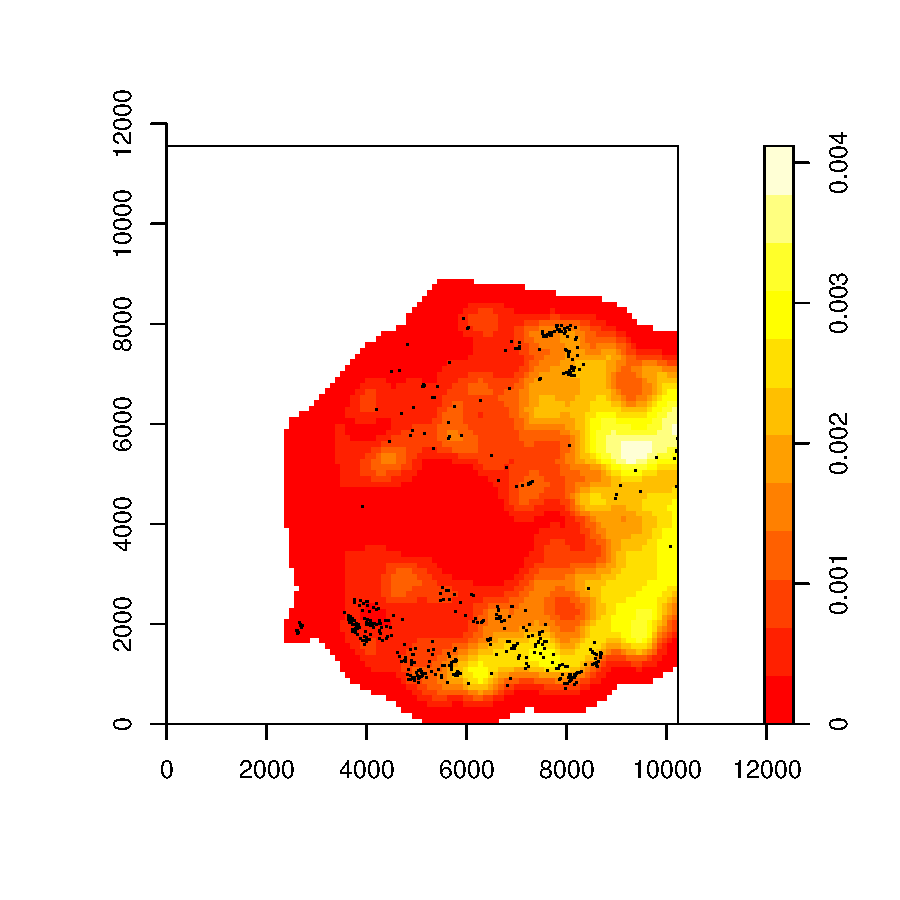
\includegraphics[scale=.5]{Fig2healthyDC.pdf}
  \end{figure}
\end{frame}

\begin{frame}{Breast Cancer Data: Survival}
  \begin{figure}
    \centering
    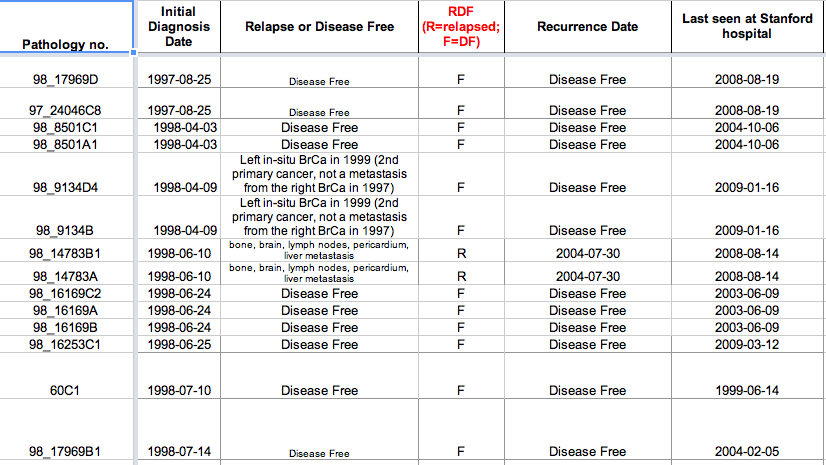
\includegraphics[scale=.5]{survival.png}
  \end{figure}
\end{frame}

\begin{frame}{Breast Cancer Data: Medical}
  \begin{figure}
    \centering
    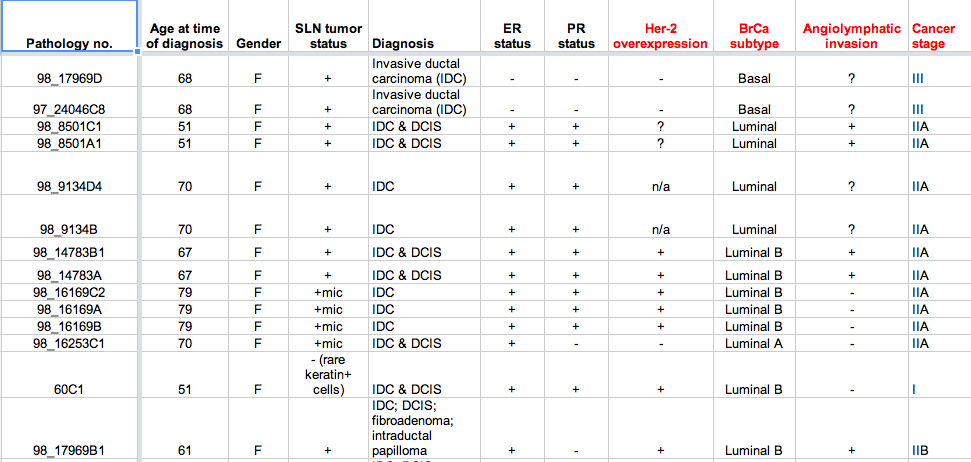
\includegraphics[scale=.5]{medical.png}
  \end{figure}
\end{frame}

\begin{frame}{Breast Cancer Study}
  \begin{itemize}
  \item How do you deal with the data integration problem? \pause
  \item Kernel methods \pause
  \item Are there any differences (spatial, medical) between women who
    relapse and those who remain disease free? \pause
  \item Two-sample tests
  \end{itemize}
\end{frame}

\begin{frame}{Friedman's Two-Sample Test}
  $\{\mathbf{x}_i\}_1^N$ from $p(\mathbf{x})$ and
  $\{\mathbf{z}_i\}_1^M$ from $q(\mathbf{z})$ testing \\
  $\mathcal{H}_A$: $p \neq q$ against $\mathcal{H}_0$: $p = q$ \pause
  \begin{enumerate}
  \item Pool the two samples $\{\mathbf{u}_i\}_1^{N+M} =
    \{\mathbf{x}_i\}_1^{N} \cup \{\mathbf{z}_i\}_1^{M}$. \pause
  \item Assign label $y_i = 1$ to the first group and $y_i = -1$ to
    the second group. \pause
  \item Apply a binary classification learning machine $f$ to the training
    data to score the observations $\{s_i = f(\mathbf{u}_i)\}_1^{N+M}$. \pause
  \item Calculate a univariate two-sample test statistic
    $T = T(\{s_i\}_1^N,\{s_i\}_{N+1}^{N+M})$. \pause
  \item Determine the permutation null distribution of the above
    statistic to yield a p-value.
  \end{enumerate}
\end{frame}

\begin{frame}{Permutation $t$-test Connection}
  With univariate data and linear scoring functions/kernels, Friedman's test reduces
  to the permutation $t$-test (normal convergence result).  \pause
  With multivariate/non-vectorial/heterogeneous data and arbitrary kernels, null distribution
  is consistent with the Normal.
\end{frame}

\begin{frame}{Other Work}
  \begin{itemize}
  \item Fisher (1935) \cite{fisher1935design} proposed distribution-free
    randomization test.  \pause
  \item Lehmann \cite{lehmann1999elements} proved a normal convergence
    result for the randomization distribution. \pause
  \item Bentkus et al. \cite{bentkus1996berry}, Shao
    \cite{shao2005explicit} proved Berry-Esseen bounds for
    Student's $t$-statistic in independent case.
  \end{itemize}
\end{frame}

\begin{frame}{Stein's Method and the Randomization Distribution}
  Let $\Phi(t)$ denote the standard normal CDF.

  Can we get a bound on
  \begin{equation*}
    \sup_{t \in \mathbb{R}} |P(T \leq t) - \Phi(t)|?
  \end{equation*}
  \pause

  $\mathcal{O}(N^{-1/4})$ with mild conditions on the data
  and $\mathcal{O}(N^{-1/2})$ with an additional condition
\end{frame}

\begin{frame}{Other Results}
  \begin{theorem}[Berry-Esseen]
  Suppose $X_1, \ldots, X_n$ are i.i.d. random variables with
  $\E X_i = 0$, $\E X_i^2 = \sigma^2 > 0$, and $\E |X_i|^3 = \rho
  < \infty$.  Let $F_n(x)$ denote the CDF of standardized sample mean
  of the $X_i$.  Then
  \begin{align*}
    \sup_x |F_n(x) - \Phi(x)| &\leq \frac{0.33477(\rho + 0.429\sigma^3)}{\sigma^3 \sqrt{n}} \\ \pause
    &= \frac{C}{\sqrt{n}} f(\rho, \sigma). \pause
  \end{align*}
  \end{theorem}
  Note that $\rho$ and $\sigma$ are fixed as $n \to \infty$.
\end{frame}

\begin{frame}{Other Results}
  \begin{theorem}[Hoeffding, Stein]
    Let $A = \{a_{ij}\}_{i, j \in \{1, \ldots, n\}}$ be a square array of
      numbers such that $\sum_j a_{ij} = 0$ for all $i$, $\sum_i
      a_{ij} = 0$ for all $j$, and $\sum_i \sum_j a_{ij}^2 = n - 1$.
      Then with $F_n(x) = P(\sum_i a_{i\Pi(i)} \leq x)$,
  \begin{align*}
    |F_n(x) - \Phi(x)| &\leq \frac{C}{\sqrt{n}}
    \left (
      \sqrt{\sum_{i,j}a_{ij}^4} + \sqrt{\sum_{i,j}|a_{ij}|^3}
    \right ) \\ \pause
    &= \frac{C}{\sqrt{n}} f(A). \pause
  \end{align*}
  \end{theorem}
  Given a sampling scheme for $A$, $f(A)$ must be $\mathcal{O}(1)$ to have rate $\mathcal{O}(n^{-1/2})$.
\end{frame}

\begin{frame}{Exchangeable Pair}
  Assume $M = N$.  Fix data $\{u_1, \ldots, u_N,
  u_{N+1}, \ldots, u_{2N}\}$.  $\Pi$ is a uniformly random permutation, and let
  \begin{equation*}
    T = T \left (\{u_{\Pi(i)}\}_{i=1}^{N},
      \{u_{\Pi(i)}\}_{i=N+1}^{2N} \right).
  \end{equation*}
  \pause

  Let $(I, J) = (i, j)$ w.p. $\frac{1}{N^2}$ for $1 \leq i \leq N$ and
  $N + 1 \leq j \leq 2N$.  Then
  \begin{equation*}
    T' = T \left (\{u_{\Pi \circ (I, J) (i)}\}_{i=1}^{N},
      \{u_{\Pi \circ (I, J) (i)}\}_{i=N+1}^{2N} \right).
  \end{equation*}
  \pause

  $T$ and $T'$ form an exchangeable pair.
\end{frame}

% \begin{frame}{Main Theorem}
% \begin{theorem}
%   If $T$, $T'$ are mean 0, exchangeable random variables with variance
%   $\E[T^2]$ satisfying
%   \begin{equation*}
%     \E[T'-T|T] = -\lambda(T-R)
%   \end{equation*}
%   for some $\lambda \in (0,1)$ and some random variable $R$, then
%   $\sup_{t \in \mathbb{R}} |P(T \leq t) - \Phi(t)|$ is bounded by
%   \begin{equation*}
%     \begin{split}
%       &(2\pi)^{-1/4} \sqrt{\frac{\E |T'-T|^3}{\lambda}}
%       + \frac{1}{2\lambda} \sqrt{\var (\E [(T'-T)^2|T])} \\
%       &|\E T^2 - 1| + \E |TR| + \E |R|
%     \end{split}
%   \end{equation*}
% \end{theorem}
% \end{frame}

\begin{frame}{Main Theorem}
\begin{theorem}
  If $T$, $T'$ are mean 0, exchangeable random variables with variance
  $\E[T^2]$ satisfying
  \begin{equation*}
    \E[T'-T|T] = -\lambda(T-R)
  \end{equation*}
  for some $\lambda \in (0,1)$ and some random variable $R$, then
  $\sup_{t \in \mathbb{R}} |P(T \leq t) - \Phi(t)|$ is bounded by
  \begin{align*}
    &\color{red}{\underbrace{(2\pi)^{-1/4} \sqrt{\frac{\E |T'-T|^3}{\lambda}}}_{\leq N^{-1/4} f_1({\bf u})}}
    \onslide<2->{
    \color{black}{+ \underbrace{\frac{1}{2\lambda} \sqrt{\var (\E [(T'-T)^2|T])}}_{\leq N^{-1} f_2({\bf u})}} \\
      &\underbrace{|\E T^2 - 1|}_{\leq N^{-1} f_3({\bf u})} + \underbrace{\E |TR|}_{\leq N^{-1/2} f_4({\bf u})} +
      \underbrace{\E |R|}_{\leq N^{-1/2} f_5({\bf u})}
    }
    \onslide<3->{\leq N^{-1/4} f_6({\bf u})}
  \end{align*}
\end{theorem}
\end{frame}

\begin{frame}{Main Theorem (Improved Rate)}
\begin{theorem}
  If in addition $|T'-T| \leq \delta$,
  $\sup_{t \in \mathbb{R}} |P(T \leq t) - \Phi(t)|$ is bounded by
  \begin{align*}
    &\color{red}{\underbrace{\frac{.41 \delta^3}{\lambda}}_{\leq N^{-1/2} c''^\ast_1}} \color{black}{+} \,
    \color{red}{\underbrace{3 \delta (\sqrt{\E T^2} + \E |R|)}_{\leq N^{-1} f'_1({\bf u})^\ast}} \,
    \onslide<2->{
      \color{black}{+ \underbrace{\frac{1}{2\lambda} \sqrt{\var (\E [(T'-T)^2|T])}}_{\leq N^{-1} f_2({\bf u})}} \\
      &\underbrace{|\E T^2 - 1|}_{\leq N^{-1} f_3({\bf u})} + \underbrace{\E |TR|}_{\leq N^{-1/2} f_4({\bf u})} +
      \underbrace{\E |R|}_{\leq N^{-1/2} f_5({\bf u})}
    }
    \onslide<3->{\leq N^{-1/2} f'_6({\bf u})^\ast}
  \end{align*}
\end{theorem}
${}^\ast$ if $\delta < c'_1 N^{-1/2}$
\end{frame}

\begin{frame}{Simulated Bounds}
  \begin{center}
    \resizebox{12.0cm}{!}{
      % Created by tikzDevice version 0.6.2-92-0ad2792 on 2013-03-31 12:41:54
% !TEX encoding = UTF-8 Unicode
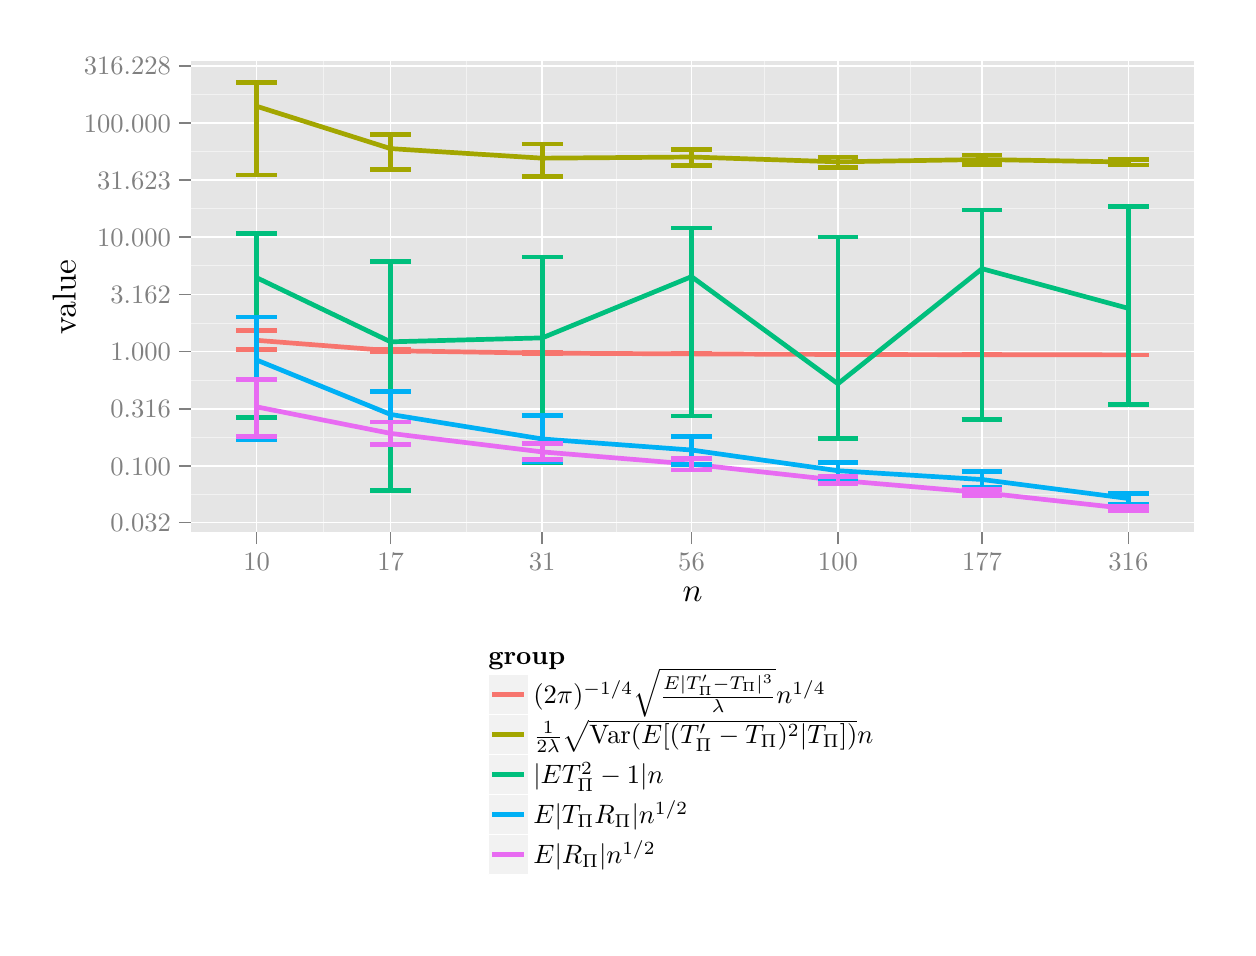
\begin{tikzpicture}[x=1pt,y=1pt]
\definecolor[named]{fillColor}{rgb}{1.00,1.00,1.00}
\path[use as bounding box,fill=fillColor,fill opacity=0.00] (0,0) rectangle (433.62,325.21);
\begin{scope}
\path[clip] (  0.00,  0.00) rectangle (433.62,325.21);
\definecolor[named]{drawColor}{rgb}{1.00,1.00,1.00}
\definecolor[named]{fillColor}{rgb}{1.00,1.00,1.00}

\path[draw=drawColor,line width= 0.6pt,line join=round,line cap=round,fill=fillColor] (  0.00,  0.00) rectangle (433.62,325.21);
\end{scope}
\begin{scope}
\path[clip] ( 58.88,142.81) rectangle (421.57,313.17);
\definecolor[named]{fillColor}{rgb}{0.90,0.90,0.90}

\path[fill=fillColor] ( 58.88,142.81) rectangle (421.57,313.17);
\definecolor[named]{drawColor}{rgb}{0.95,0.95,0.95}

\path[draw=drawColor,line width= 0.3pt,line join=round] ( 58.88,156.64) --
	(421.57,156.64);

\path[draw=drawColor,line width= 0.3pt,line join=round] ( 58.88,177.18) --
	(421.57,177.18);

\path[draw=drawColor,line width= 0.3pt,line join=round] ( 58.88,197.84) --
	(421.57,197.84);

\path[draw=drawColor,line width= 0.3pt,line join=round] ( 58.88,218.50) --
	(421.57,218.50);

\path[draw=drawColor,line width= 0.3pt,line join=round] ( 58.88,239.15) --
	(421.57,239.15);

\path[draw=drawColor,line width= 0.3pt,line join=round] ( 58.88,259.81) --
	(421.57,259.81);

\path[draw=drawColor,line width= 0.3pt,line join=round] ( 58.88,280.46) --
	(421.57,280.46);

\path[draw=drawColor,line width= 0.3pt,line join=round] ( 58.88,301.12) --
	(421.57,301.12);

\path[draw=drawColor,line width= 0.3pt,line join=round] (106.92,142.81) --
	(106.92,313.17);

\path[draw=drawColor,line width= 0.3pt,line join=round] (158.53,142.81) --
	(158.53,313.17);

\path[draw=drawColor,line width= 0.3pt,line join=round] (212.91,142.81) --
	(212.91,313.17);

\path[draw=drawColor,line width= 0.3pt,line join=round] (266.33,142.81) --
	(266.33,313.17);

\path[draw=drawColor,line width= 0.3pt,line join=round] (318.82,142.81) --
	(318.82,313.17);

\path[draw=drawColor,line width= 0.3pt,line join=round] (371.30,142.81) --
	(371.30,313.17);
\definecolor[named]{drawColor}{rgb}{1.00,1.00,1.00}

\path[draw=drawColor,line width= 0.6pt,line join=round] ( 58.88,146.42) --
	(421.57,146.42);

\path[draw=drawColor,line width= 0.6pt,line join=round] ( 58.88,166.86) --
	(421.57,166.86);

\path[draw=drawColor,line width= 0.6pt,line join=round] ( 58.88,187.50) --
	(421.57,187.50);

\path[draw=drawColor,line width= 0.6pt,line join=round] ( 58.88,208.17) --
	(421.57,208.17);

\path[draw=drawColor,line width= 0.6pt,line join=round] ( 58.88,228.82) --
	(421.57,228.82);

\path[draw=drawColor,line width= 0.6pt,line join=round] ( 58.88,249.48) --
	(421.57,249.48);

\path[draw=drawColor,line width= 0.6pt,line join=round] ( 58.88,270.13) --
	(421.57,270.13);

\path[draw=drawColor,line width= 0.6pt,line join=round] ( 58.88,290.79) --
	(421.57,290.79);

\path[draw=drawColor,line width= 0.6pt,line join=round] ( 58.88,311.44) --
	(421.57,311.44);

\path[draw=drawColor,line width= 0.6pt,line join=round] ( 82.72,142.81) --
	( 82.72,313.17);

\path[draw=drawColor,line width= 0.6pt,line join=round] (131.13,142.81) --
	(131.13,313.17);

\path[draw=drawColor,line width= 0.6pt,line join=round] (185.93,142.81) --
	(185.93,313.17);

\path[draw=drawColor,line width= 0.6pt,line join=round] (239.88,142.81) --
	(239.88,313.17);

\path[draw=drawColor,line width= 0.6pt,line join=round] (292.78,142.81) --
	(292.78,313.17);

\path[draw=drawColor,line width= 0.6pt,line join=round] (344.86,142.81) --
	(344.86,313.17);

\path[draw=drawColor,line width= 0.6pt,line join=round] (397.74,142.81) --
	(397.74,313.17);
\definecolor[named]{drawColor}{rgb}{0.97,0.46,0.43}

\path[draw=drawColor,line width= 1.7pt,line join=round] ( 82.72,212.23) --
	(131.13,208.47) --
	(185.93,207.59) --
	(239.88,207.33) --
	(292.78,207.11) --
	(344.86,207.03) --
	(397.74,206.97);
\definecolor[named]{drawColor}{rgb}{0.64,0.65,0.00}

\path[draw=drawColor,line width= 1.7pt,line join=round] ( 82.72,296.81) --
	(131.13,281.50) --
	(185.93,278.05) --
	(239.88,278.47) --
	(292.78,276.73) --
	(344.86,277.57) --
	(397.74,276.65);
\definecolor[named]{drawColor}{rgb}{0.00,0.75,0.49}

\path[draw=drawColor,line width= 1.7pt,line join=round] ( 82.72,234.87) --
	(131.13,211.69) --
	(185.93,213.11) --
	(239.88,235.24) --
	(292.78,196.53) --
	(344.86,238.11) --
	(397.74,223.78);
\definecolor[named]{drawColor}{rgb}{0.00,0.69,0.96}

\path[draw=drawColor,line width= 1.7pt,line join=round] ( 82.72,205.12) --
	(131.13,185.45) --
	(185.93,176.58) --
	(239.88,172.59) --
	(292.78,165.11) --
	(344.86,161.94) --
	(397.74,155.08);
\definecolor[named]{drawColor}{rgb}{0.91,0.42,0.95}

\path[draw=drawColor,line width= 1.7pt,line join=round] ( 82.72,188.19) --
	(131.13,178.60) --
	(185.93,171.91) --
	(239.88,167.48) --
	(292.78,161.66) --
	(344.86,157.21) --
	(397.74,151.36);
\definecolor[named]{drawColor}{rgb}{0.97,0.46,0.43}

\path[draw=drawColor,line width= 1.7pt,line join=round] ( 75.37,215.79) --
	( 90.07,215.79);

\path[draw=drawColor,line width= 1.7pt,line join=round] ( 82.72,215.79) --
	( 82.72,209.03);

\path[draw=drawColor,line width= 1.7pt,line join=round] ( 75.37,209.03) --
	( 90.07,209.03);

\path[draw=drawColor,line width= 1.7pt,line join=round] (123.78,209.01) --
	(138.48,209.01);

\path[draw=drawColor,line width= 1.7pt,line join=round] (131.13,209.01) --
	(131.13,207.96);

\path[draw=drawColor,line width= 1.7pt,line join=round] (123.78,207.96) --
	(138.48,207.96);

\path[draw=drawColor,line width= 1.7pt,line join=round] (178.58,207.78) --
	(193.28,207.78);

\path[draw=drawColor,line width= 1.7pt,line join=round] (185.93,207.78) --
	(185.93,207.43);

\path[draw=drawColor,line width= 1.7pt,line join=round] (178.58,207.43) --
	(193.28,207.43);

\path[draw=drawColor,line width= 1.7pt,line join=round] (232.53,207.40) --
	(247.23,207.40);

\path[draw=drawColor,line width= 1.7pt,line join=round] (239.88,207.40) --
	(239.88,207.26);

\path[draw=drawColor,line width= 1.7pt,line join=round] (232.53,207.26) --
	(247.23,207.26);

\path[draw=drawColor,line width= 1.7pt,line join=round] (285.42,207.14) --
	(300.13,207.14);

\path[draw=drawColor,line width= 1.7pt,line join=round] (292.78,207.14) --
	(292.78,207.09);

\path[draw=drawColor,line width= 1.7pt,line join=round] (285.42,207.09) --
	(300.13,207.09);

\path[draw=drawColor,line width= 1.7pt,line join=round] (337.51,207.04) --
	(352.22,207.04);

\path[draw=drawColor,line width= 1.7pt,line join=round] (344.86,207.04) --
	(344.86,207.01);

\path[draw=drawColor,line width= 1.7pt,line join=round] (337.51,207.01) --
	(352.22,207.01);

\path[draw=drawColor,line width= 1.7pt,line join=round] (390.39,206.98) --
	(405.09,206.98);

\path[draw=drawColor,line width= 1.7pt,line join=round] (397.74,206.98) --
	(397.74,206.97);

\path[draw=drawColor,line width= 1.7pt,line join=round] (390.39,206.97) --
	(405.09,206.97);
\definecolor[named]{drawColor}{rgb}{0.64,0.65,0.00}

\path[draw=drawColor,line width= 1.7pt,line join=round] ( 75.37,305.43) --
	( 90.07,305.43);

\path[draw=drawColor,line width= 1.7pt,line join=round] ( 82.72,305.43) --
	( 82.72,272.00);

\path[draw=drawColor,line width= 1.7pt,line join=round] ( 75.37,272.00) --
	( 90.07,272.00);

\path[draw=drawColor,line width= 1.7pt,line join=round] (123.78,286.57) --
	(138.48,286.57);

\path[draw=drawColor,line width= 1.7pt,line join=round] (131.13,286.57) --
	(131.13,273.88);

\path[draw=drawColor,line width= 1.7pt,line join=round] (123.78,273.88) --
	(138.48,273.88);

\path[draw=drawColor,line width= 1.7pt,line join=round] (178.58,283.20) --
	(193.28,283.20);

\path[draw=drawColor,line width= 1.7pt,line join=round] (185.93,283.20) --
	(185.93,271.44);

\path[draw=drawColor,line width= 1.7pt,line join=round] (178.58,271.44) --
	(193.28,271.44);

\path[draw=drawColor,line width= 1.7pt,line join=round] (232.53,281.15) --
	(247.23,281.15);

\path[draw=drawColor,line width= 1.7pt,line join=round] (239.88,281.15) --
	(239.88,275.41);

\path[draw=drawColor,line width= 1.7pt,line join=round] (232.53,275.41) --
	(247.23,275.41);

\path[draw=drawColor,line width= 1.7pt,line join=round] (285.42,278.48) --
	(300.13,278.48);

\path[draw=drawColor,line width= 1.7pt,line join=round] (292.78,278.48) --
	(292.78,274.78);

\path[draw=drawColor,line width= 1.7pt,line join=round] (285.42,274.78) --
	(300.13,274.78);

\path[draw=drawColor,line width= 1.7pt,line join=round] (337.51,279.20) --
	(352.22,279.20);

\path[draw=drawColor,line width= 1.7pt,line join=round] (344.86,279.20) --
	(344.86,275.70);

\path[draw=drawColor,line width= 1.7pt,line join=round] (337.51,275.70) --
	(352.22,275.70);

\path[draw=drawColor,line width= 1.7pt,line join=round] (390.39,277.66) --
	(405.09,277.66);

\path[draw=drawColor,line width= 1.7pt,line join=round] (397.74,277.66) --
	(397.74,275.55);

\path[draw=drawColor,line width= 1.7pt,line join=round] (390.39,275.55) --
	(405.09,275.55);
\definecolor[named]{drawColor}{rgb}{0.00,0.75,0.49}

\path[draw=drawColor,line width= 1.7pt,line join=round] ( 75.37,250.71) --
	( 90.07,250.71);

\path[draw=drawColor,line width= 1.7pt,line join=round] ( 82.72,250.71) --
	( 82.72,184.35);

\path[draw=drawColor,line width= 1.7pt,line join=round] ( 75.37,184.35) --
	( 90.07,184.35);

\path[draw=drawColor,line width= 1.7pt,line join=round] (123.78,240.65) --
	(138.48,240.65);

\path[draw=drawColor,line width= 1.7pt,line join=round] (131.13,240.65) --
	(131.13,157.85);

\path[draw=drawColor,line width= 1.7pt,line join=round] (123.78,157.85) --
	(138.48,157.85);

\path[draw=drawColor,line width= 1.7pt,line join=round] (178.58,242.36) --
	(193.28,242.36);

\path[draw=drawColor,line width= 1.7pt,line join=round] (185.93,242.36) --
	(185.93,168.02);

\path[draw=drawColor,line width= 1.7pt,line join=round] (178.58,168.02) --
	(193.28,168.02);

\path[draw=drawColor,line width= 1.7pt,line join=round] (232.53,252.82) --
	(247.23,252.82);

\path[draw=drawColor,line width= 1.7pt,line join=round] (239.88,252.82) --
	(239.88,184.90);

\path[draw=drawColor,line width= 1.7pt,line join=round] (232.53,184.90) --
	(247.23,184.90);

\path[draw=drawColor,line width= 1.7pt,line join=round] (285.42,249.54) --
	(300.13,249.54);

\path[draw=drawColor,line width= 1.7pt,line join=round] (292.78,249.54) --
	(292.78,176.72);

\path[draw=drawColor,line width= 1.7pt,line join=round] (285.42,176.72) --
	(300.13,176.72);

\path[draw=drawColor,line width= 1.7pt,line join=round] (337.51,259.28) --
	(352.22,259.28);

\path[draw=drawColor,line width= 1.7pt,line join=round] (344.86,259.28) --
	(344.86,183.59);

\path[draw=drawColor,line width= 1.7pt,line join=round] (337.51,183.59) --
	(352.22,183.59);

\path[draw=drawColor,line width= 1.7pt,line join=round] (390.39,260.67) --
	(405.09,260.67);

\path[draw=drawColor,line width= 1.7pt,line join=round] (397.74,260.67) --
	(397.74,189.01);

\path[draw=drawColor,line width= 1.7pt,line join=round] (390.39,189.01) --
	(405.09,189.01);
\definecolor[named]{drawColor}{rgb}{0.00,0.69,0.96}

\path[draw=drawColor,line width= 1.7pt,line join=round] ( 75.37,220.63) --
	( 90.07,220.63);

\path[draw=drawColor,line width= 1.7pt,line join=round] ( 82.72,220.63) --
	( 82.72,176.45);

\path[draw=drawColor,line width= 1.7pt,line join=round] ( 75.37,176.45) --
	( 90.07,176.45);

\path[draw=drawColor,line width= 1.7pt,line join=round] (123.78,193.86) --
	(138.48,193.86);

\path[draw=drawColor,line width= 1.7pt,line join=round] (131.13,193.86) --
	(131.13,174.67);

\path[draw=drawColor,line width= 1.7pt,line join=round] (123.78,174.67) --
	(138.48,174.67);

\path[draw=drawColor,line width= 1.7pt,line join=round] (178.58,185.02) --
	(193.28,185.02);

\path[draw=drawColor,line width= 1.7pt,line join=round] (185.93,185.02) --
	(185.93,168.34);

\path[draw=drawColor,line width= 1.7pt,line join=round] (178.58,168.34) --
	(193.28,168.34);

\path[draw=drawColor,line width= 1.7pt,line join=round] (232.53,177.45) --
	(247.23,177.45);

\path[draw=drawColor,line width= 1.7pt,line join=round] (239.88,177.45) --
	(239.88,167.34);

\path[draw=drawColor,line width= 1.7pt,line join=round] (232.53,167.34) --
	(247.23,167.34);

\path[draw=drawColor,line width= 1.7pt,line join=round] (285.42,168.13) --
	(300.13,168.13);

\path[draw=drawColor,line width= 1.7pt,line join=round] (292.78,168.13) --
	(292.78,161.90);

\path[draw=drawColor,line width= 1.7pt,line join=round] (285.42,161.90) --
	(300.13,161.90);

\path[draw=drawColor,line width= 1.7pt,line join=round] (337.51,164.95) --
	(352.22,164.95);

\path[draw=drawColor,line width= 1.7pt,line join=round] (344.86,164.95) --
	(344.86,158.98);

\path[draw=drawColor,line width= 1.7pt,line join=round] (337.51,158.98) --
	(352.22,158.98);

\path[draw=drawColor,line width= 1.7pt,line join=round] (390.39,156.99) --
	(405.09,156.99);

\path[draw=drawColor,line width= 1.7pt,line join=round] (397.74,156.99) --
	(397.74,153.12);

\path[draw=drawColor,line width= 1.7pt,line join=round] (390.39,153.12) --
	(405.09,153.12);
\definecolor[named]{drawColor}{rgb}{0.91,0.42,0.95}

\path[draw=drawColor,line width= 1.7pt,line join=round] ( 75.37,198.11) --
	( 90.07,198.11);

\path[draw=drawColor,line width= 1.7pt,line join=round] ( 82.72,198.11) --
	( 82.72,177.60);

\path[draw=drawColor,line width= 1.7pt,line join=round] ( 75.37,177.60) --
	( 90.07,177.60);

\path[draw=drawColor,line width= 1.7pt,line join=round] (123.78,182.73) --
	(138.48,182.73);

\path[draw=drawColor,line width= 1.7pt,line join=round] (131.13,182.73) --
	(131.13,174.52);

\path[draw=drawColor,line width= 1.7pt,line join=round] (123.78,174.52) --
	(138.48,174.52);

\path[draw=drawColor,line width= 1.7pt,line join=round] (178.58,175.06) --
	(193.28,175.06);

\path[draw=drawColor,line width= 1.7pt,line join=round] (185.93,175.06) --
	(185.93,169.10);

\path[draw=drawColor,line width= 1.7pt,line join=round] (178.58,169.10) --
	(193.28,169.10);

\path[draw=drawColor,line width= 1.7pt,line join=round] (232.53,169.53) --
	(247.23,169.53);

\path[draw=drawColor,line width= 1.7pt,line join=round] (239.88,169.53) --
	(239.88,165.42);

\path[draw=drawColor,line width= 1.7pt,line join=round] (232.53,165.42) --
	(247.23,165.42);

\path[draw=drawColor,line width= 1.7pt,line join=round] (285.42,162.96) --
	(300.13,162.96);

\path[draw=drawColor,line width= 1.7pt,line join=round] (292.78,162.96) --
	(292.78,160.37);

\path[draw=drawColor,line width= 1.7pt,line join=round] (285.42,160.37) --
	(300.13,160.37);

\path[draw=drawColor,line width= 1.7pt,line join=round] (337.51,158.45) --
	(352.22,158.45);

\path[draw=drawColor,line width= 1.7pt,line join=round] (344.86,158.45) --
	(344.86,156.04);

\path[draw=drawColor,line width= 1.7pt,line join=round] (337.51,156.04) --
	(352.22,156.04);

\path[draw=drawColor,line width= 1.7pt,line join=round] (390.39,152.16) --
	(405.09,152.16);

\path[draw=drawColor,line width= 1.7pt,line join=round] (397.74,152.16) --
	(397.74,150.56);

\path[draw=drawColor,line width= 1.7pt,line join=round] (390.39,150.56) --
	(405.09,150.56);
\end{scope}
\begin{scope}
\path[clip] (  0.00,  0.00) rectangle (433.62,325.21);
\definecolor[named]{drawColor}{rgb}{0.50,0.50,0.50}

\node[text=drawColor,anchor=base east,inner sep=0pt, outer sep=0pt, scale=  0.96] at ( 51.77,143.11) {0.032};

\node[text=drawColor,anchor=base east,inner sep=0pt, outer sep=0pt, scale=  0.96] at ( 51.77,163.55) {0.100};

\node[text=drawColor,anchor=base east,inner sep=0pt, outer sep=0pt, scale=  0.96] at ( 51.77,184.20) {0.316};

\node[text=drawColor,anchor=base east,inner sep=0pt, outer sep=0pt, scale=  0.96] at ( 51.77,204.86) {1.000};

\node[text=drawColor,anchor=base east,inner sep=0pt, outer sep=0pt, scale=  0.96] at ( 51.77,225.52) {3.162};

\node[text=drawColor,anchor=base east,inner sep=0pt, outer sep=0pt, scale=  0.96] at ( 51.77,246.17) {10.000};

\node[text=drawColor,anchor=base east,inner sep=0pt, outer sep=0pt, scale=  0.96] at ( 51.77,266.83) {31.623};

\node[text=drawColor,anchor=base east,inner sep=0pt, outer sep=0pt, scale=  0.96] at ( 51.77,287.48) {100.000};

\node[text=drawColor,anchor=base east,inner sep=0pt, outer sep=0pt, scale=  0.96] at ( 51.77,308.14) {316.228};
\end{scope}
\begin{scope}
\path[clip] (  0.00,  0.00) rectangle (433.62,325.21);
\definecolor[named]{drawColor}{rgb}{0.50,0.50,0.50}

\path[draw=drawColor,line width= 0.6pt,line join=round] ( 54.61,146.42) --
	( 58.88,146.42);

\path[draw=drawColor,line width= 0.6pt,line join=round] ( 54.61,166.86) --
	( 58.88,166.86);

\path[draw=drawColor,line width= 0.6pt,line join=round] ( 54.61,187.50) --
	( 58.88,187.50);

\path[draw=drawColor,line width= 0.6pt,line join=round] ( 54.61,208.17) --
	( 58.88,208.17);

\path[draw=drawColor,line width= 0.6pt,line join=round] ( 54.61,228.82) --
	( 58.88,228.82);

\path[draw=drawColor,line width= 0.6pt,line join=round] ( 54.61,249.48) --
	( 58.88,249.48);

\path[draw=drawColor,line width= 0.6pt,line join=round] ( 54.61,270.13) --
	( 58.88,270.13);

\path[draw=drawColor,line width= 0.6pt,line join=round] ( 54.61,290.79) --
	( 58.88,290.79);

\path[draw=drawColor,line width= 0.6pt,line join=round] ( 54.61,311.44) --
	( 58.88,311.44);
\end{scope}
\begin{scope}
\path[clip] (  0.00,  0.00) rectangle (433.62,325.21);
\definecolor[named]{drawColor}{rgb}{0.50,0.50,0.50}

\path[draw=drawColor,line width= 0.6pt,line join=round] ( 82.72,138.55) --
	( 82.72,142.81);

\path[draw=drawColor,line width= 0.6pt,line join=round] (131.13,138.55) --
	(131.13,142.81);

\path[draw=drawColor,line width= 0.6pt,line join=round] (185.93,138.55) --
	(185.93,142.81);

\path[draw=drawColor,line width= 0.6pt,line join=round] (239.88,138.55) --
	(239.88,142.81);

\path[draw=drawColor,line width= 0.6pt,line join=round] (292.78,138.55) --
	(292.78,142.81);

\path[draw=drawColor,line width= 0.6pt,line join=round] (344.86,138.55) --
	(344.86,142.81);

\path[draw=drawColor,line width= 0.6pt,line join=round] (397.74,138.55) --
	(397.74,142.81);
\end{scope}
\begin{scope}
\path[clip] (  0.00,  0.00) rectangle (433.62,325.21);
\definecolor[named]{drawColor}{rgb}{0.50,0.50,0.50}

\node[text=drawColor,anchor=base,inner sep=0pt, outer sep=0pt, scale=  0.96] at ( 82.72,129.09) {10};

\node[text=drawColor,anchor=base,inner sep=0pt, outer sep=0pt, scale=  0.96] at (131.13,129.09) {17};

\node[text=drawColor,anchor=base,inner sep=0pt, outer sep=0pt, scale=  0.96] at (185.93,129.09) {31};

\node[text=drawColor,anchor=base,inner sep=0pt, outer sep=0pt, scale=  0.96] at (239.88,129.09) {56};

\node[text=drawColor,anchor=base,inner sep=0pt, outer sep=0pt, scale=  0.96] at (292.78,129.09) {100};

\node[text=drawColor,anchor=base,inner sep=0pt, outer sep=0pt, scale=  0.96] at (344.86,129.09) {177};

\node[text=drawColor,anchor=base,inner sep=0pt, outer sep=0pt, scale=  0.96] at (397.74,129.09) {316};
\end{scope}
\begin{scope}
\path[clip] (  0.00,  0.00) rectangle (433.62,325.21);
\definecolor[named]{drawColor}{rgb}{0.00,0.00,0.00}

\node[text=drawColor,anchor=base,inner sep=0pt, outer sep=0pt, scale=  1.20] at (240.23,117.81) {$n$};
\end{scope}
\begin{scope}
\path[clip] (  0.00,  0.00) rectangle (433.62,325.21);
\definecolor[named]{drawColor}{rgb}{0.00,0.00,0.00}

\node[text=drawColor,rotate= 90.00,anchor=base,inner sep=0pt, outer sep=0pt, scale=  1.20] at ( 17.30,227.99) {value};
\end{scope}
\begin{scope}
\path[clip] (  0.00,  0.00) rectangle (433.62,325.21);
\definecolor[named]{fillColor}{rgb}{1.00,1.00,1.00}

\path[fill=fillColor] (162.21, 14.89) rectangle (318.25,105.93);
\end{scope}
\begin{scope}
\path[clip] (  0.00,  0.00) rectangle (433.62,325.21);
\definecolor[named]{drawColor}{rgb}{0.00,0.00,0.00}

\node[text=drawColor,anchor=base west,inner sep=0pt, outer sep=0pt, scale=  0.96] at (166.47, 95.04) {\bfseries group};
\end{scope}
\begin{scope}
\path[clip] (  0.00,  0.00) rectangle (433.62,325.21);
\definecolor[named]{drawColor}{rgb}{1.00,1.00,1.00}
\definecolor[named]{fillColor}{rgb}{0.95,0.95,0.95}

\path[draw=drawColor,line width= 0.6pt,line join=round,line cap=round,fill=fillColor] (166.47, 76.97) rectangle (180.93, 91.43);
\end{scope}
\begin{scope}
\path[clip] (  0.00,  0.00) rectangle (433.62,325.21);
\definecolor[named]{drawColor}{rgb}{0.97,0.46,0.43}

\path[draw=drawColor,line width= 1.7pt,line join=round] (167.92, 84.20) -- (179.48, 84.20);
\end{scope}
\begin{scope}
\path[clip] (  0.00,  0.00) rectangle (433.62,325.21);
\definecolor[named]{drawColor}{rgb}{0.97,0.46,0.43}

\path[draw=drawColor,line width= 1.7pt,line join=round] (167.92, 84.20) -- (179.48, 84.20);
\end{scope}
\begin{scope}
\path[clip] (  0.00,  0.00) rectangle (433.62,325.21);
\definecolor[named]{drawColor}{rgb}{1.00,1.00,1.00}
\definecolor[named]{fillColor}{rgb}{0.95,0.95,0.95}

\path[draw=drawColor,line width= 0.6pt,line join=round,line cap=round,fill=fillColor] (166.47, 62.52) rectangle (180.93, 76.97);
\end{scope}
\begin{scope}
\path[clip] (  0.00,  0.00) rectangle (433.62,325.21);
\definecolor[named]{drawColor}{rgb}{0.64,0.65,0.00}

\path[draw=drawColor,line width= 1.7pt,line join=round] (167.92, 69.75) -- (179.48, 69.75);
\end{scope}
\begin{scope}
\path[clip] (  0.00,  0.00) rectangle (433.62,325.21);
\definecolor[named]{drawColor}{rgb}{0.64,0.65,0.00}

\path[draw=drawColor,line width= 1.7pt,line join=round] (167.92, 69.75) -- (179.48, 69.75);
\end{scope}
\begin{scope}
\path[clip] (  0.00,  0.00) rectangle (433.62,325.21);
\definecolor[named]{drawColor}{rgb}{1.00,1.00,1.00}
\definecolor[named]{fillColor}{rgb}{0.95,0.95,0.95}

\path[draw=drawColor,line width= 0.6pt,line join=round,line cap=round,fill=fillColor] (166.47, 48.07) rectangle (180.93, 62.52);
\end{scope}
\begin{scope}
\path[clip] (  0.00,  0.00) rectangle (433.62,325.21);
\definecolor[named]{drawColor}{rgb}{0.00,0.75,0.49}

\path[draw=drawColor,line width= 1.7pt,line join=round] (167.92, 55.29) -- (179.48, 55.29);
\end{scope}
\begin{scope}
\path[clip] (  0.00,  0.00) rectangle (433.62,325.21);
\definecolor[named]{drawColor}{rgb}{0.00,0.75,0.49}

\path[draw=drawColor,line width= 1.7pt,line join=round] (167.92, 55.29) -- (179.48, 55.29);
\end{scope}
\begin{scope}
\path[clip] (  0.00,  0.00) rectangle (433.62,325.21);
\definecolor[named]{drawColor}{rgb}{1.00,1.00,1.00}
\definecolor[named]{fillColor}{rgb}{0.95,0.95,0.95}

\path[draw=drawColor,line width= 0.6pt,line join=round,line cap=round,fill=fillColor] (166.47, 33.61) rectangle (180.93, 48.07);
\end{scope}
\begin{scope}
\path[clip] (  0.00,  0.00) rectangle (433.62,325.21);
\definecolor[named]{drawColor}{rgb}{0.00,0.69,0.96}

\path[draw=drawColor,line width= 1.7pt,line join=round] (167.92, 40.84) -- (179.48, 40.84);
\end{scope}
\begin{scope}
\path[clip] (  0.00,  0.00) rectangle (433.62,325.21);
\definecolor[named]{drawColor}{rgb}{0.00,0.69,0.96}

\path[draw=drawColor,line width= 1.7pt,line join=round] (167.92, 40.84) -- (179.48, 40.84);
\end{scope}
\begin{scope}
\path[clip] (  0.00,  0.00) rectangle (433.62,325.21);
\definecolor[named]{drawColor}{rgb}{1.00,1.00,1.00}
\definecolor[named]{fillColor}{rgb}{0.95,0.95,0.95}

\path[draw=drawColor,line width= 0.6pt,line join=round,line cap=round,fill=fillColor] (166.47, 19.16) rectangle (180.93, 33.61);
\end{scope}
\begin{scope}
\path[clip] (  0.00,  0.00) rectangle (433.62,325.21);
\definecolor[named]{drawColor}{rgb}{0.91,0.42,0.95}

\path[draw=drawColor,line width= 1.7pt,line join=round] (167.92, 26.39) -- (179.48, 26.39);
\end{scope}
\begin{scope}
\path[clip] (  0.00,  0.00) rectangle (433.62,325.21);
\definecolor[named]{drawColor}{rgb}{0.91,0.42,0.95}

\path[draw=drawColor,line width= 1.7pt,line join=round] (167.92, 26.39) -- (179.48, 26.39);
\end{scope}
\begin{scope}
\path[clip] (  0.00,  0.00) rectangle (433.62,325.21);
\definecolor[named]{drawColor}{rgb}{0.00,0.00,0.00}

\node[text=drawColor,anchor=base west,inner sep=0pt, outer sep=0pt, scale=  0.96] at (182.73, 80.90) {$(2\pi)^{-1/4}\sqrt{\frac{\mathbb{E}|T'_{\Pi}-T_{\Pi}|^3}{\lambda}}n^{1/4}\quad $};
\end{scope}
\begin{scope}
\path[clip] (  0.00,  0.00) rectangle (433.62,325.21);
\definecolor[named]{drawColor}{rgb}{0.00,0.00,0.00}

\node[text=drawColor,anchor=base west,inner sep=0pt, outer sep=0pt, scale=  0.96] at (182.73, 66.44) {$\frac{1}{2\lambda}\sqrt{\mathrm{Var}(\mathbb{E}[(T'_{\Pi}-T_{\Pi})^2|T_{\Pi}])}n\quad $};
\end{scope}
\begin{scope}
\path[clip] (  0.00,  0.00) rectangle (433.62,325.21);
\definecolor[named]{drawColor}{rgb}{0.00,0.00,0.00}

\node[text=drawColor,anchor=base west,inner sep=0pt, outer sep=0pt, scale=  0.96] at (182.73, 51.99) {$|\mathbb{E}T_{\Pi}^2-1|n\quad $};
\end{scope}
\begin{scope}
\path[clip] (  0.00,  0.00) rectangle (433.62,325.21);
\definecolor[named]{drawColor}{rgb}{0.00,0.00,0.00}

\node[text=drawColor,anchor=base west,inner sep=0pt, outer sep=0pt, scale=  0.96] at (182.73, 37.53) {$\mathbb{E}|T_{\Pi}R_{\Pi}|n^{1/2}\quad $};
\end{scope}
\begin{scope}
\path[clip] (  0.00,  0.00) rectangle (433.62,325.21);
\definecolor[named]{drawColor}{rgb}{0.00,0.00,0.00}

\node[text=drawColor,anchor=base west,inner sep=0pt, outer sep=0pt, scale=  0.96] at (182.73, 23.08) {$\mathbb{E}|R_{\Pi}|n^{1/2}\quad $};
\end{scope}
\end{tikzpicture}

    }
  \end{center}
\end{frame}

\begin{frame}{Simulated Bounds (Improved Rate)}
  \begin{center}
    \resizebox{10.0cm}{!}{
      % Created by tikzDevice version 0.6.2-92-0ad2792 on 2013-05-05 16:12:42
% !TEX encoding = UTF-8 Unicode
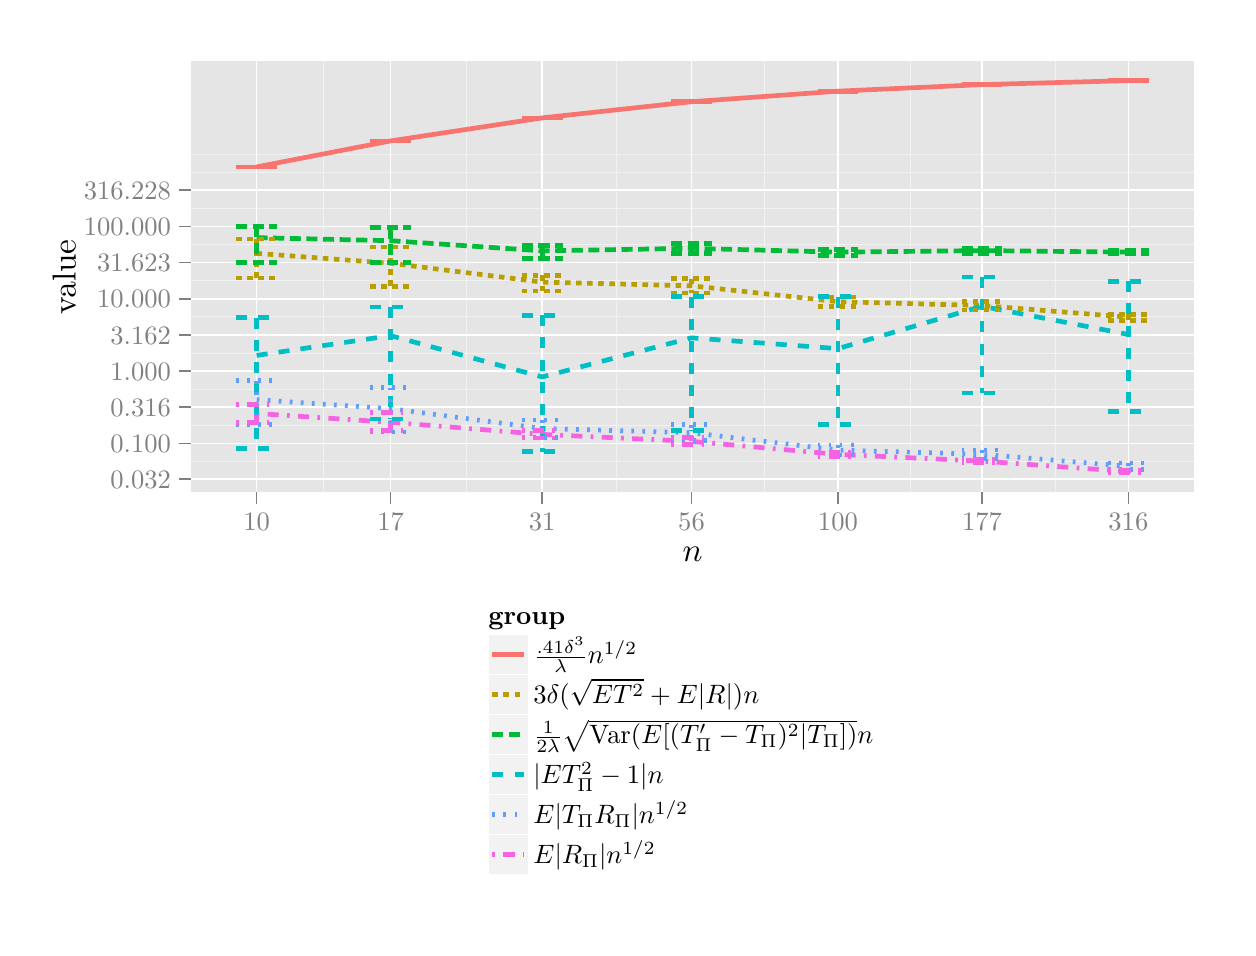
\begin{tikzpicture}[x=1pt,y=1pt]
\definecolor[named]{fillColor}{rgb}{1.00,1.00,1.00}
\path[use as bounding box,fill=fillColor,fill opacity=0.00] (0,0) rectangle (433.62,325.21);
\begin{scope}
\path[clip] (  0.00,  0.00) rectangle (433.62,325.21);
\definecolor[named]{drawColor}{rgb}{1.00,1.00,1.00}
\definecolor[named]{fillColor}{rgb}{1.00,1.00,1.00}

\path[draw=drawColor,line width= 0.6pt,line join=round,line cap=round,fill=fillColor] (  0.00,  0.00) rectangle (433.62,325.21);
\end{scope}
\begin{scope}
\path[clip] ( 58.88,157.27) rectangle (421.57,313.17);
\definecolor[named]{fillColor}{rgb}{0.90,0.90,0.90}

\path[fill=fillColor] ( 58.88,157.27) rectangle (421.57,313.17);
\definecolor[named]{drawColor}{rgb}{0.95,0.95,0.95}

\path[draw=drawColor,line width= 0.3pt,line join=round] ( 58.88,168.50) --
	(421.57,168.50);

\path[draw=drawColor,line width= 0.3pt,line join=round] ( 58.88,181.50) --
	(421.57,181.50);

\path[draw=drawColor,line width= 0.3pt,line join=round] ( 58.88,194.57) --
	(421.57,194.57);

\path[draw=drawColor,line width= 0.3pt,line join=round] ( 58.88,207.64) --
	(421.57,207.64);

\path[draw=drawColor,line width= 0.3pt,line join=round] ( 58.88,220.71) --
	(421.57,220.71);

\path[draw=drawColor,line width= 0.3pt,line join=round] ( 58.88,233.78) --
	(421.57,233.78);

\path[draw=drawColor,line width= 0.3pt,line join=round] ( 58.88,246.85) --
	(421.57,246.85);

\path[draw=drawColor,line width= 0.3pt,line join=round] ( 58.88,259.92) --
	(421.57,259.92);

\path[draw=drawColor,line width= 0.3pt,line join=round] ( 58.88,272.93) --
	(421.57,272.93);

\path[draw=drawColor,line width= 0.3pt,line join=round] ( 58.88,279.39) --
	(421.57,279.39);

\path[draw=drawColor,line width= 0.3pt,line join=round] (106.92,157.27) --
	(106.92,313.17);

\path[draw=drawColor,line width= 0.3pt,line join=round] (158.53,157.27) --
	(158.53,313.17);

\path[draw=drawColor,line width= 0.3pt,line join=round] (212.91,157.27) --
	(212.91,313.17);

\path[draw=drawColor,line width= 0.3pt,line join=round] (266.33,157.27) --
	(266.33,313.17);

\path[draw=drawColor,line width= 0.3pt,line join=round] (318.82,157.27) --
	(318.82,313.17);

\path[draw=drawColor,line width= 0.3pt,line join=round] (371.30,157.27) --
	(371.30,313.17);
\definecolor[named]{drawColor}{rgb}{1.00,1.00,1.00}

\path[draw=drawColor,line width= 0.6pt,line join=round] ( 58.88,162.03) --
	(421.57,162.03);

\path[draw=drawColor,line width= 0.6pt,line join=round] ( 58.88,174.97) --
	(421.57,174.97);

\path[draw=drawColor,line width= 0.6pt,line join=round] ( 58.88,188.03) --
	(421.57,188.03);

\path[draw=drawColor,line width= 0.6pt,line join=round] ( 58.88,201.11) --
	(421.57,201.11);

\path[draw=drawColor,line width= 0.6pt,line join=round] ( 58.88,214.18) --
	(421.57,214.18);

\path[draw=drawColor,line width= 0.6pt,line join=round] ( 58.88,227.25) --
	(421.57,227.25);

\path[draw=drawColor,line width= 0.6pt,line join=round] ( 58.88,240.32) --
	(421.57,240.32);

\path[draw=drawColor,line width= 0.6pt,line join=round] ( 58.88,253.39) --
	(421.57,253.39);

\path[draw=drawColor,line width= 0.6pt,line join=round] ( 58.88,266.46) --
	(421.57,266.46);

\path[draw=drawColor,line width= 0.6pt,line join=round] ( 82.72,157.27) --
	( 82.72,313.17);

\path[draw=drawColor,line width= 0.6pt,line join=round] (131.13,157.27) --
	(131.13,313.17);

\path[draw=drawColor,line width= 0.6pt,line join=round] (185.93,157.27) --
	(185.93,313.17);

\path[draw=drawColor,line width= 0.6pt,line join=round] (239.88,157.27) --
	(239.88,313.17);

\path[draw=drawColor,line width= 0.6pt,line join=round] (292.78,157.27) --
	(292.78,313.17);

\path[draw=drawColor,line width= 0.6pt,line join=round] (344.86,157.27) --
	(344.86,313.17);

\path[draw=drawColor,line width= 0.6pt,line join=round] (397.74,157.27) --
	(397.74,313.17);
\definecolor[named]{drawColor}{rgb}{0.97,0.46,0.43}

\path[draw=drawColor,line width= 1.7pt,line join=round] ( 82.72,274.89) --
	(131.13,284.28) --
	(185.93,292.61) --
	(239.88,298.45) --
	(292.78,302.26) --
	(344.86,304.63) --
	(397.74,306.08);
\definecolor[named]{drawColor}{rgb}{0.72,0.62,0.00}

\path[draw=drawColor,line width= 1.7pt,dash pattern=on 2pt off 2pt ,line join=round] ( 82.72,243.66) --
	(131.13,240.08) --
	(185.93,233.27) --
	(239.88,231.93) --
	(292.78,226.20) --
	(344.86,224.80) --
	(397.74,220.60);
\definecolor[named]{drawColor}{rgb}{0.00,0.73,0.22}

\path[draw=drawColor,line width= 1.7pt,dash pattern=on 4pt off 2pt ,line join=round] ( 82.72,249.33) --
	(131.13,248.23) --
	(185.93,244.56) --
	(239.88,245.48) --
	(292.78,244.09) --
	(344.86,244.65) --
	(397.74,244.10);
\definecolor[named]{drawColor}{rgb}{0.00,0.75,0.77}

\path[draw=drawColor,line width= 1.7pt,dash pattern=on 4pt off 4pt ,line join=round] ( 82.72,206.77) --
	(131.13,213.92) --
	(185.93,199.00) --
	(239.88,213.13) --
	(292.78,209.23) --
	(344.86,224.54) --
	(397.74,214.35);
\definecolor[named]{drawColor}{rgb}{0.38,0.61,1.00}

\path[draw=drawColor,line width= 1.7pt,dash pattern=on 1pt off 3pt ,line join=round] ( 82.72,190.78) --
	(131.13,187.54) --
	(185.93,180.37) --
	(239.88,178.84) --
	(292.78,172.56) --
	(344.86,171.06) --
	(397.74,166.69);
\definecolor[named]{drawColor}{rgb}{0.96,0.39,0.89}

\path[draw=drawColor,line width= 1.7pt,dash pattern=on 1pt off 3pt on 4pt off 3pt ,line join=round] ( 82.72,185.80) --
	(131.13,182.62) --
	(185.93,178.24) --
	(239.88,175.72) --
	(292.78,171.01) --
	(344.86,168.59) --
	(397.74,164.80);
\definecolor[named]{drawColor}{rgb}{0.97,0.46,0.43}

\path[draw=drawColor,line width= 1.7pt,line join=round] ( 75.37,274.89) --
	( 90.07,274.89);

\path[draw=drawColor,line width= 1.7pt,line join=round] ( 82.72,274.89) --
	( 82.72,274.89);

\path[draw=drawColor,line width= 1.7pt,line join=round] ( 75.37,274.89) --
	( 90.07,274.89);

\path[draw=drawColor,line width= 1.7pt,line join=round] (123.78,284.28) --
	(138.48,284.28);

\path[draw=drawColor,line width= 1.7pt,line join=round] (131.13,284.28) --
	(131.13,284.28);

\path[draw=drawColor,line width= 1.7pt,line join=round] (123.78,284.28) --
	(138.48,284.28);

\path[draw=drawColor,line width= 1.7pt,line join=round] (178.58,292.61) --
	(193.28,292.61);

\path[draw=drawColor,line width= 1.7pt,line join=round] (185.93,292.61) --
	(185.93,292.61);

\path[draw=drawColor,line width= 1.7pt,line join=round] (178.58,292.61) --
	(193.28,292.61);

\path[draw=drawColor,line width= 1.7pt,line join=round] (232.53,298.45) --
	(247.23,298.45);

\path[draw=drawColor,line width= 1.7pt,line join=round] (239.88,298.45) --
	(239.88,298.45);

\path[draw=drawColor,line width= 1.7pt,line join=round] (232.53,298.45) --
	(247.23,298.45);

\path[draw=drawColor,line width= 1.7pt,line join=round] (285.42,302.26) --
	(300.13,302.26);

\path[draw=drawColor,line width= 1.7pt,line join=round] (292.78,302.26) --
	(292.78,302.26);

\path[draw=drawColor,line width= 1.7pt,line join=round] (285.42,302.26) --
	(300.13,302.26);

\path[draw=drawColor,line width= 1.7pt,line join=round] (337.51,304.63) --
	(352.22,304.63);

\path[draw=drawColor,line width= 1.7pt,line join=round] (344.86,304.63) --
	(344.86,304.63);

\path[draw=drawColor,line width= 1.7pt,line join=round] (337.51,304.63) --
	(352.22,304.63);

\path[draw=drawColor,line width= 1.7pt,line join=round] (390.39,306.08) --
	(405.09,306.08);

\path[draw=drawColor,line width= 1.7pt,line join=round] (397.74,306.08) --
	(397.74,306.08);

\path[draw=drawColor,line width= 1.7pt,line join=round] (390.39,306.08) --
	(405.09,306.08);
\definecolor[named]{drawColor}{rgb}{0.72,0.62,0.00}

\path[draw=drawColor,line width= 1.7pt,dash pattern=on 2pt off 2pt ,line join=round] ( 75.37,248.87) --
	( 90.07,248.87);

\path[draw=drawColor,line width= 1.7pt,dash pattern=on 2pt off 2pt ,line join=round] ( 82.72,248.87) --
	( 82.72,234.74);

\path[draw=drawColor,line width= 1.7pt,dash pattern=on 2pt off 2pt ,line join=round] ( 75.37,234.74) --
	( 90.07,234.74);

\path[draw=drawColor,line width= 1.7pt,dash pattern=on 2pt off 2pt ,line join=round] (123.78,245.97) --
	(138.48,245.97);

\path[draw=drawColor,line width= 1.7pt,dash pattern=on 2pt off 2pt ,line join=round] (131.13,245.97) --
	(131.13,231.80);

\path[draw=drawColor,line width= 1.7pt,dash pattern=on 2pt off 2pt ,line join=round] (123.78,231.80) --
	(138.48,231.80);

\path[draw=drawColor,line width= 1.7pt,dash pattern=on 2pt off 2pt ,line join=round] (178.58,235.77) --
	(193.28,235.77);

\path[draw=drawColor,line width= 1.7pt,dash pattern=on 2pt off 2pt ,line join=round] (185.93,235.77) --
	(185.93,230.09);

\path[draw=drawColor,line width= 1.7pt,dash pattern=on 2pt off 2pt ,line join=round] (178.58,230.09) --
	(193.28,230.09);

\path[draw=drawColor,line width= 1.7pt,dash pattern=on 2pt off 2pt ,line join=round] (232.53,234.49) --
	(247.23,234.49);

\path[draw=drawColor,line width= 1.7pt,dash pattern=on 2pt off 2pt ,line join=round] (239.88,234.49) --
	(239.88,229.34);

\path[draw=drawColor,line width= 1.7pt,dash pattern=on 2pt off 2pt ,line join=round] (232.53,229.34) --
	(247.23,229.34);

\path[draw=drawColor,line width= 1.7pt,dash pattern=on 2pt off 2pt ,line join=round] (285.42,227.86) --
	(300.13,227.86);

\path[draw=drawColor,line width= 1.7pt,dash pattern=on 2pt off 2pt ,line join=round] (292.78,227.86) --
	(292.78,224.41);

\path[draw=drawColor,line width= 1.7pt,dash pattern=on 2pt off 2pt ,line join=round] (285.42,224.41) --
	(300.13,224.41);

\path[draw=drawColor,line width= 1.7pt,dash pattern=on 2pt off 2pt ,line join=round] (337.51,226.29) --
	(352.22,226.29);

\path[draw=drawColor,line width= 1.7pt,dash pattern=on 2pt off 2pt ,line join=round] (344.86,226.29) --
	(344.86,223.23);

\path[draw=drawColor,line width= 1.7pt,dash pattern=on 2pt off 2pt ,line join=round] (337.51,223.23) --
	(352.22,223.23);

\path[draw=drawColor,line width= 1.7pt,dash pattern=on 2pt off 2pt ,line join=round] (390.39,221.68) --
	(405.09,221.68);

\path[draw=drawColor,line width= 1.7pt,dash pattern=on 2pt off 2pt ,line join=round] (397.74,221.68) --
	(397.74,219.48);

\path[draw=drawColor,line width= 1.7pt,dash pattern=on 2pt off 2pt ,line join=round] (390.39,219.48) --
	(405.09,219.48);
\definecolor[named]{drawColor}{rgb}{0.00,0.73,0.22}

\path[draw=drawColor,line width= 1.7pt,dash pattern=on 4pt off 2pt ,line join=round] ( 75.37,253.42) --
	( 90.07,253.42);

\path[draw=drawColor,line width= 1.7pt,dash pattern=on 4pt off 2pt ,line join=round] ( 82.72,253.42) --
	( 82.72,240.31);

\path[draw=drawColor,line width= 1.7pt,dash pattern=on 4pt off 2pt ,line join=round] ( 75.37,240.31) --
	( 90.07,240.31);

\path[draw=drawColor,line width= 1.7pt,dash pattern=on 4pt off 2pt ,line join=round] (123.78,252.95) --
	(138.48,252.95);

\path[draw=drawColor,line width= 1.7pt,dash pattern=on 4pt off 2pt ,line join=round] (131.13,252.95) --
	(131.13,240.33);

\path[draw=drawColor,line width= 1.7pt,dash pattern=on 4pt off 2pt ,line join=round] (123.78,240.33) --
	(138.48,240.33);

\path[draw=drawColor,line width= 1.7pt,dash pattern=on 4pt off 2pt ,line join=round] (178.58,246.46) --
	(193.28,246.46);

\path[draw=drawColor,line width= 1.7pt,dash pattern=on 4pt off 2pt ,line join=round] (185.93,246.46) --
	(185.93,241.88);

\path[draw=drawColor,line width= 1.7pt,dash pattern=on 4pt off 2pt ,line join=round] (178.58,241.88) --
	(193.28,241.88);

\path[draw=drawColor,line width= 1.7pt,dash pattern=on 4pt off 2pt ,line join=round] (232.53,247.11) --
	(247.23,247.11);

\path[draw=drawColor,line width= 1.7pt,dash pattern=on 4pt off 2pt ,line join=round] (239.88,247.11) --
	(239.88,243.71);

\path[draw=drawColor,line width= 1.7pt,dash pattern=on 4pt off 2pt ,line join=round] (232.53,243.71) --
	(247.23,243.71);

\path[draw=drawColor,line width= 1.7pt,dash pattern=on 4pt off 2pt ,line join=round] (285.42,245.16) --
	(300.13,245.16);

\path[draw=drawColor,line width= 1.7pt,dash pattern=on 4pt off 2pt ,line join=round] (292.78,245.16) --
	(292.78,242.89);

\path[draw=drawColor,line width= 1.7pt,dash pattern=on 4pt off 2pt ,line join=round] (285.42,242.89) --
	(300.13,242.89);

\path[draw=drawColor,line width= 1.7pt,dash pattern=on 4pt off 2pt ,line join=round] (337.51,245.53) --
	(352.22,245.53);

\path[draw=drawColor,line width= 1.7pt,dash pattern=on 4pt off 2pt ,line join=round] (344.86,245.53) --
	(344.86,243.65);

\path[draw=drawColor,line width= 1.7pt,dash pattern=on 4pt off 2pt ,line join=round] (337.51,243.65) --
	(352.22,243.65);

\path[draw=drawColor,line width= 1.7pt,dash pattern=on 4pt off 2pt ,line join=round] (390.39,244.74) --
	(405.09,244.74);

\path[draw=drawColor,line width= 1.7pt,dash pattern=on 4pt off 2pt ,line join=round] (397.74,244.74) --
	(397.74,243.44);

\path[draw=drawColor,line width= 1.7pt,dash pattern=on 4pt off 2pt ,line join=round] (390.39,243.44) --
	(405.09,243.44);
\definecolor[named]{drawColor}{rgb}{0.00,0.75,0.77}

\path[draw=drawColor,line width= 1.7pt,dash pattern=on 4pt off 4pt ,line join=round] ( 75.37,220.42) --
	( 90.07,220.42);

\path[draw=drawColor,line width= 1.7pt,dash pattern=on 4pt off 4pt ,line join=round] ( 82.72,220.42) --
	( 82.72,173.09);

\path[draw=drawColor,line width= 1.7pt,dash pattern=on 4pt off 4pt ,line join=round] ( 75.37,173.09) --
	( 90.07,173.09);

\path[draw=drawColor,line width= 1.7pt,dash pattern=on 4pt off 4pt ,line join=round] (123.78,224.22) --
	(138.48,224.22);

\path[draw=drawColor,line width= 1.7pt,dash pattern=on 4pt off 4pt ,line join=round] (131.13,224.22) --
	(131.13,183.80);

\path[draw=drawColor,line width= 1.7pt,dash pattern=on 4pt off 4pt ,line join=round] (123.78,183.80) --
	(138.48,183.80);

\path[draw=drawColor,line width= 1.7pt,dash pattern=on 4pt off 4pt ,line join=round] (178.58,221.29) --
	(193.28,221.29);

\path[draw=drawColor,line width= 1.7pt,dash pattern=on 4pt off 4pt ,line join=round] (185.93,221.29) --
	(185.93,172.02);

\path[draw=drawColor,line width= 1.7pt,dash pattern=on 4pt off 4pt ,line join=round] (178.58,172.02) --
	(193.28,172.02);

\path[draw=drawColor,line width= 1.7pt,dash pattern=on 4pt off 4pt ,line join=round] (232.53,228.00) --
	(247.23,228.00);

\path[draw=drawColor,line width= 1.7pt,dash pattern=on 4pt off 4pt ,line join=round] (239.88,228.00) --
	(239.88,179.75);

\path[draw=drawColor,line width= 1.7pt,dash pattern=on 4pt off 4pt ,line join=round] (232.53,179.75) --
	(247.23,179.75);

\path[draw=drawColor,line width= 1.7pt,dash pattern=on 4pt off 4pt ,line join=round] (285.42,228.02) --
	(300.13,228.02);

\path[draw=drawColor,line width= 1.7pt,dash pattern=on 4pt off 4pt ,line join=round] (292.78,228.02) --
	(292.78,181.91);

\path[draw=drawColor,line width= 1.7pt,dash pattern=on 4pt off 4pt ,line join=round] (285.42,181.91) --
	(300.13,181.91);

\path[draw=drawColor,line width= 1.7pt,dash pattern=on 4pt off 4pt ,line join=round] (337.51,235.07) --
	(352.22,235.07);

\path[draw=drawColor,line width= 1.7pt,dash pattern=on 4pt off 4pt ,line join=round] (344.86,235.07) --
	(344.86,193.17);

\path[draw=drawColor,line width= 1.7pt,dash pattern=on 4pt off 4pt ,line join=round] (337.51,193.17) --
	(352.22,193.17);

\path[draw=drawColor,line width= 1.7pt,dash pattern=on 4pt off 4pt ,line join=round] (390.39,233.58) --
	(405.09,233.58);

\path[draw=drawColor,line width= 1.7pt,dash pattern=on 4pt off 4pt ,line join=round] (397.74,233.58) --
	(397.74,186.61);

\path[draw=drawColor,line width= 1.7pt,dash pattern=on 4pt off 4pt ,line join=round] (390.39,186.61) --
	(405.09,186.61);
\definecolor[named]{drawColor}{rgb}{0.38,0.61,1.00}

\path[draw=drawColor,line width= 1.7pt,dash pattern=on 1pt off 3pt ,line join=round] ( 75.37,197.61) --
	( 90.07,197.61);

\path[draw=drawColor,line width= 1.7pt,dash pattern=on 1pt off 3pt ,line join=round] ( 82.72,197.61) --
	( 82.72,181.75);

\path[draw=drawColor,line width= 1.7pt,dash pattern=on 1pt off 3pt ,line join=round] ( 75.37,181.75) --
	( 90.07,181.75);

\path[draw=drawColor,line width= 1.7pt,dash pattern=on 1pt off 3pt ,line join=round] (123.78,195.10) --
	(138.48,195.10);

\path[draw=drawColor,line width= 1.7pt,dash pattern=on 1pt off 3pt ,line join=round] (131.13,195.10) --
	(131.13,179.14);

\path[draw=drawColor,line width= 1.7pt,dash pattern=on 1pt off 3pt ,line join=round] (123.78,179.14) --
	(138.48,179.14);

\path[draw=drawColor,line width= 1.7pt,dash pattern=on 1pt off 3pt ,line join=round] (178.58,183.39) --
	(193.28,183.39);

\path[draw=drawColor,line width= 1.7pt,dash pattern=on 1pt off 3pt ,line join=round] (185.93,183.39) --
	(185.93,177.06);

\path[draw=drawColor,line width= 1.7pt,dash pattern=on 1pt off 3pt ,line join=round] (178.58,177.06) --
	(193.28,177.06);

\path[draw=drawColor,line width= 1.7pt,dash pattern=on 1pt off 3pt ,line join=round] (232.53,181.72) --
	(247.23,181.72);

\path[draw=drawColor,line width= 1.7pt,dash pattern=on 1pt off 3pt ,line join=round] (239.88,181.72) --
	(239.88,176.01);

\path[draw=drawColor,line width= 1.7pt,dash pattern=on 1pt off 3pt ,line join=round] (232.53,176.01) --
	(247.23,176.01);

\path[draw=drawColor,line width= 1.7pt,dash pattern=on 1pt off 3pt ,line join=round] (285.42,174.38) --
	(300.13,174.38);

\path[draw=drawColor,line width= 1.7pt,dash pattern=on 1pt off 3pt ,line join=round] (292.78,174.38) --
	(292.78,170.76);

\path[draw=drawColor,line width= 1.7pt,dash pattern=on 1pt off 3pt ,line join=round] (285.42,170.76) --
	(300.13,170.76);

\path[draw=drawColor,line width= 1.7pt,dash pattern=on 1pt off 3pt ,line join=round] (337.51,172.65) --
	(352.22,172.65);

\path[draw=drawColor,line width= 1.7pt,dash pattern=on 1pt off 3pt ,line join=round] (344.86,172.65) --
	(344.86,169.46);

\path[draw=drawColor,line width= 1.7pt,dash pattern=on 1pt off 3pt ,line join=round] (337.51,169.46) --
	(352.22,169.46);

\path[draw=drawColor,line width= 1.7pt,dash pattern=on 1pt off 3pt ,line join=round] (390.39,167.90) --
	(405.09,167.90);

\path[draw=drawColor,line width= 1.7pt,dash pattern=on 1pt off 3pt ,line join=round] (397.74,167.90) --
	(397.74,165.53);

\path[draw=drawColor,line width= 1.7pt,dash pattern=on 1pt off 3pt ,line join=round] (390.39,165.53) --
	(405.09,165.53);
\definecolor[named]{drawColor}{rgb}{0.96,0.39,0.89}

\path[draw=drawColor,line width= 1.7pt,dash pattern=on 1pt off 3pt on 4pt off 3pt ,line join=round] ( 75.37,189.04) --
	( 90.07,189.04);

\path[draw=drawColor,line width= 1.7pt,dash pattern=on 1pt off 3pt on 4pt off 3pt ,line join=round] ( 82.72,189.04) --
	( 82.72,182.53);

\path[draw=drawColor,line width= 1.7pt,dash pattern=on 1pt off 3pt on 4pt off 3pt ,line join=round] ( 75.37,182.53) --
	( 90.07,182.53);

\path[draw=drawColor,line width= 1.7pt,dash pattern=on 1pt off 3pt on 4pt off 3pt ,line join=round] (123.78,186.20) --
	(138.48,186.20);

\path[draw=drawColor,line width= 1.7pt,dash pattern=on 1pt off 3pt on 4pt off 3pt ,line join=round] (131.13,186.20) --
	(131.13,179.73);

\path[draw=drawColor,line width= 1.7pt,dash pattern=on 1pt off 3pt on 4pt off 3pt ,line join=round] (123.78,179.73) --
	(138.48,179.73);

\path[draw=drawColor,line width= 1.7pt,dash pattern=on 1pt off 3pt on 4pt off 3pt ,line join=round] (178.58,179.63) --
	(193.28,179.63);

\path[draw=drawColor,line width= 1.7pt,dash pattern=on 1pt off 3pt on 4pt off 3pt ,line join=round] (185.93,179.63) --
	(185.93,176.94);

\path[draw=drawColor,line width= 1.7pt,dash pattern=on 1pt off 3pt on 4pt off 3pt ,line join=round] (178.58,176.94) --
	(193.28,176.94);

\path[draw=drawColor,line width= 1.7pt,dash pattern=on 1pt off 3pt on 4pt off 3pt ,line join=round] (232.53,176.99) --
	(247.23,176.99);

\path[draw=drawColor,line width= 1.7pt,dash pattern=on 1pt off 3pt on 4pt off 3pt ,line join=round] (239.88,176.99) --
	(239.88,174.54);

\path[draw=drawColor,line width= 1.7pt,dash pattern=on 1pt off 3pt on 4pt off 3pt ,line join=round] (232.53,174.54) --
	(247.23,174.54);

\path[draw=drawColor,line width= 1.7pt,dash pattern=on 1pt off 3pt on 4pt off 3pt ,line join=round] (285.42,171.79) --
	(300.13,171.79);

\path[draw=drawColor,line width= 1.7pt,dash pattern=on 1pt off 3pt on 4pt off 3pt ,line join=round] (292.78,171.79) --
	(292.78,170.31);

\path[draw=drawColor,line width= 1.7pt,dash pattern=on 1pt off 3pt on 4pt off 3pt ,line join=round] (285.42,170.31) --
	(300.13,170.31);

\path[draw=drawColor,line width= 1.7pt,dash pattern=on 1pt off 3pt on 4pt off 3pt ,line join=round] (337.51,169.29) --
	(352.22,169.29);

\path[draw=drawColor,line width= 1.7pt,dash pattern=on 1pt off 3pt on 4pt off 3pt ,line join=round] (344.86,169.29) --
	(344.86,167.97);

\path[draw=drawColor,line width= 1.7pt,dash pattern=on 1pt off 3pt on 4pt off 3pt ,line join=round] (337.51,167.97) --
	(352.22,167.97);

\path[draw=drawColor,line width= 1.7pt,dash pattern=on 1pt off 3pt on 4pt off 3pt ,line join=round] (390.39,165.25) --
	(405.09,165.25);

\path[draw=drawColor,line width= 1.7pt,dash pattern=on 1pt off 3pt on 4pt off 3pt ,line join=round] (397.74,165.25) --
	(397.74,164.35);

\path[draw=drawColor,line width= 1.7pt,dash pattern=on 1pt off 3pt on 4pt off 3pt ,line join=round] (390.39,164.35) --
	(405.09,164.35);
\end{scope}
\begin{scope}
\path[clip] (  0.00,  0.00) rectangle (433.62,325.21);
\definecolor[named]{drawColor}{rgb}{0.50,0.50,0.50}

\node[text=drawColor,anchor=base east,inner sep=0pt, outer sep=0pt, scale=  0.96] at ( 51.77,158.73) {0.032};

\node[text=drawColor,anchor=base east,inner sep=0pt, outer sep=0pt, scale=  0.96] at ( 51.77,171.66) {0.100};

\node[text=drawColor,anchor=base east,inner sep=0pt, outer sep=0pt, scale=  0.96] at ( 51.77,184.72) {0.316};

\node[text=drawColor,anchor=base east,inner sep=0pt, outer sep=0pt, scale=  0.96] at ( 51.77,197.80) {1.000};

\node[text=drawColor,anchor=base east,inner sep=0pt, outer sep=0pt, scale=  0.96] at ( 51.77,210.87) {3.162};

\node[text=drawColor,anchor=base east,inner sep=0pt, outer sep=0pt, scale=  0.96] at ( 51.77,223.94) {10.000};

\node[text=drawColor,anchor=base east,inner sep=0pt, outer sep=0pt, scale=  0.96] at ( 51.77,237.01) {31.623};

\node[text=drawColor,anchor=base east,inner sep=0pt, outer sep=0pt, scale=  0.96] at ( 51.77,250.08) {100.000};

\node[text=drawColor,anchor=base east,inner sep=0pt, outer sep=0pt, scale=  0.96] at ( 51.77,263.15) {316.228};
\end{scope}
\begin{scope}
\path[clip] (  0.00,  0.00) rectangle (433.62,325.21);
\definecolor[named]{drawColor}{rgb}{0.50,0.50,0.50}

\path[draw=drawColor,line width= 0.6pt,line join=round] ( 54.61,162.03) --
	( 58.88,162.03);

\path[draw=drawColor,line width= 0.6pt,line join=round] ( 54.61,174.97) --
	( 58.88,174.97);

\path[draw=drawColor,line width= 0.6pt,line join=round] ( 54.61,188.03) --
	( 58.88,188.03);

\path[draw=drawColor,line width= 0.6pt,line join=round] ( 54.61,201.11) --
	( 58.88,201.11);

\path[draw=drawColor,line width= 0.6pt,line join=round] ( 54.61,214.18) --
	( 58.88,214.18);

\path[draw=drawColor,line width= 0.6pt,line join=round] ( 54.61,227.25) --
	( 58.88,227.25);

\path[draw=drawColor,line width= 0.6pt,line join=round] ( 54.61,240.32) --
	( 58.88,240.32);

\path[draw=drawColor,line width= 0.6pt,line join=round] ( 54.61,253.39) --
	( 58.88,253.39);

\path[draw=drawColor,line width= 0.6pt,line join=round] ( 54.61,266.46) --
	( 58.88,266.46);
\end{scope}
\begin{scope}
\path[clip] (  0.00,  0.00) rectangle (433.62,325.21);
\definecolor[named]{drawColor}{rgb}{0.50,0.50,0.50}

\path[draw=drawColor,line width= 0.6pt,line join=round] ( 82.72,153.00) --
	( 82.72,157.27);

\path[draw=drawColor,line width= 0.6pt,line join=round] (131.13,153.00) --
	(131.13,157.27);

\path[draw=drawColor,line width= 0.6pt,line join=round] (185.93,153.00) --
	(185.93,157.27);

\path[draw=drawColor,line width= 0.6pt,line join=round] (239.88,153.00) --
	(239.88,157.27);

\path[draw=drawColor,line width= 0.6pt,line join=round] (292.78,153.00) --
	(292.78,157.27);

\path[draw=drawColor,line width= 0.6pt,line join=round] (344.86,153.00) --
	(344.86,157.27);

\path[draw=drawColor,line width= 0.6pt,line join=round] (397.74,153.00) --
	(397.74,157.27);
\end{scope}
\begin{scope}
\path[clip] (  0.00,  0.00) rectangle (433.62,325.21);
\definecolor[named]{drawColor}{rgb}{0.50,0.50,0.50}

\node[text=drawColor,anchor=base,inner sep=0pt, outer sep=0pt, scale=  0.96] at ( 82.72,143.54) {10};

\node[text=drawColor,anchor=base,inner sep=0pt, outer sep=0pt, scale=  0.96] at (131.13,143.54) {17};

\node[text=drawColor,anchor=base,inner sep=0pt, outer sep=0pt, scale=  0.96] at (185.93,143.54) {31};

\node[text=drawColor,anchor=base,inner sep=0pt, outer sep=0pt, scale=  0.96] at (239.88,143.54) {56};

\node[text=drawColor,anchor=base,inner sep=0pt, outer sep=0pt, scale=  0.96] at (292.78,143.54) {100};

\node[text=drawColor,anchor=base,inner sep=0pt, outer sep=0pt, scale=  0.96] at (344.86,143.54) {177};

\node[text=drawColor,anchor=base,inner sep=0pt, outer sep=0pt, scale=  0.96] at (397.74,143.54) {316};
\end{scope}
\begin{scope}
\path[clip] (  0.00,  0.00) rectangle (433.62,325.21);
\definecolor[named]{drawColor}{rgb}{0.00,0.00,0.00}

\node[text=drawColor,anchor=base,inner sep=0pt, outer sep=0pt, scale=  1.20] at (240.23,132.27) {$n$};
\end{scope}
\begin{scope}
\path[clip] (  0.00,  0.00) rectangle (433.62,325.21);
\definecolor[named]{drawColor}{rgb}{0.00,0.00,0.00}

\node[text=drawColor,rotate= 90.00,anchor=base,inner sep=0pt, outer sep=0pt, scale=  1.20] at ( 17.30,235.22) {value};
\end{scope}
\begin{scope}
\path[clip] (  0.00,  0.00) rectangle (433.62,325.21);
\definecolor[named]{fillColor}{rgb}{1.00,1.00,1.00}

\path[fill=fillColor] (162.21, 14.89) rectangle (318.25,120.39);
\end{scope}
\begin{scope}
\path[clip] (  0.00,  0.00) rectangle (433.62,325.21);
\definecolor[named]{drawColor}{rgb}{0.00,0.00,0.00}

\node[text=drawColor,anchor=base west,inner sep=0pt, outer sep=0pt, scale=  0.96] at (166.47,109.50) {\bfseries group};
\end{scope}
\begin{scope}
\path[clip] (  0.00,  0.00) rectangle (433.62,325.21);
\definecolor[named]{drawColor}{rgb}{1.00,1.00,1.00}
\definecolor[named]{fillColor}{rgb}{0.95,0.95,0.95}

\path[draw=drawColor,line width= 0.6pt,line join=round,line cap=round,fill=fillColor] (166.47, 91.43) rectangle (180.93,105.88);
\end{scope}
\begin{scope}
\path[clip] (  0.00,  0.00) rectangle (433.62,325.21);
\definecolor[named]{drawColor}{rgb}{0.97,0.46,0.43}

\path[draw=drawColor,line width= 1.7pt,line join=round] (167.92, 98.66) -- (179.48, 98.66);
\end{scope}
\begin{scope}
\path[clip] (  0.00,  0.00) rectangle (433.62,325.21);
\definecolor[named]{drawColor}{rgb}{0.97,0.46,0.43}

\path[draw=drawColor,line width= 1.7pt,line join=round] (167.92, 98.66) -- (179.48, 98.66);
\end{scope}
\begin{scope}
\path[clip] (  0.00,  0.00) rectangle (433.62,325.21);
\definecolor[named]{drawColor}{rgb}{1.00,1.00,1.00}
\definecolor[named]{fillColor}{rgb}{0.95,0.95,0.95}

\path[draw=drawColor,line width= 0.6pt,line join=round,line cap=round,fill=fillColor] (166.47, 76.97) rectangle (180.93, 91.43);
\end{scope}
\begin{scope}
\path[clip] (  0.00,  0.00) rectangle (433.62,325.21);
\definecolor[named]{drawColor}{rgb}{0.72,0.62,0.00}

\path[draw=drawColor,line width= 1.7pt,dash pattern=on 2pt off 2pt ,line join=round] (167.92, 84.20) -- (179.48, 84.20);
\end{scope}
\begin{scope}
\path[clip] (  0.00,  0.00) rectangle (433.62,325.21);
\definecolor[named]{drawColor}{rgb}{0.72,0.62,0.00}

\path[draw=drawColor,line width= 1.7pt,dash pattern=on 2pt off 2pt ,line join=round] (167.92, 84.20) -- (179.48, 84.20);
\end{scope}
\begin{scope}
\path[clip] (  0.00,  0.00) rectangle (433.62,325.21);
\definecolor[named]{drawColor}{rgb}{1.00,1.00,1.00}
\definecolor[named]{fillColor}{rgb}{0.95,0.95,0.95}

\path[draw=drawColor,line width= 0.6pt,line join=round,line cap=round,fill=fillColor] (166.47, 62.52) rectangle (180.93, 76.97);
\end{scope}
\begin{scope}
\path[clip] (  0.00,  0.00) rectangle (433.62,325.21);
\definecolor[named]{drawColor}{rgb}{0.00,0.73,0.22}

\path[draw=drawColor,line width= 1.7pt,dash pattern=on 4pt off 2pt ,line join=round] (167.92, 69.75) -- (179.48, 69.75);
\end{scope}
\begin{scope}
\path[clip] (  0.00,  0.00) rectangle (433.62,325.21);
\definecolor[named]{drawColor}{rgb}{0.00,0.73,0.22}

\path[draw=drawColor,line width= 1.7pt,dash pattern=on 4pt off 2pt ,line join=round] (167.92, 69.75) -- (179.48, 69.75);
\end{scope}
\begin{scope}
\path[clip] (  0.00,  0.00) rectangle (433.62,325.21);
\definecolor[named]{drawColor}{rgb}{1.00,1.00,1.00}
\definecolor[named]{fillColor}{rgb}{0.95,0.95,0.95}

\path[draw=drawColor,line width= 0.6pt,line join=round,line cap=round,fill=fillColor] (166.47, 48.07) rectangle (180.93, 62.52);
\end{scope}
\begin{scope}
\path[clip] (  0.00,  0.00) rectangle (433.62,325.21);
\definecolor[named]{drawColor}{rgb}{0.00,0.75,0.77}

\path[draw=drawColor,line width= 1.7pt,dash pattern=on 4pt off 4pt ,line join=round] (167.92, 55.29) -- (179.48, 55.29);
\end{scope}
\begin{scope}
\path[clip] (  0.00,  0.00) rectangle (433.62,325.21);
\definecolor[named]{drawColor}{rgb}{0.00,0.75,0.77}

\path[draw=drawColor,line width= 1.7pt,dash pattern=on 4pt off 4pt ,line join=round] (167.92, 55.29) -- (179.48, 55.29);
\end{scope}
\begin{scope}
\path[clip] (  0.00,  0.00) rectangle (433.62,325.21);
\definecolor[named]{drawColor}{rgb}{1.00,1.00,1.00}
\definecolor[named]{fillColor}{rgb}{0.95,0.95,0.95}

\path[draw=drawColor,line width= 0.6pt,line join=round,line cap=round,fill=fillColor] (166.47, 33.61) rectangle (180.93, 48.07);
\end{scope}
\begin{scope}
\path[clip] (  0.00,  0.00) rectangle (433.62,325.21);
\definecolor[named]{drawColor}{rgb}{0.38,0.61,1.00}

\path[draw=drawColor,line width= 1.7pt,dash pattern=on 1pt off 3pt ,line join=round] (167.92, 40.84) -- (179.48, 40.84);
\end{scope}
\begin{scope}
\path[clip] (  0.00,  0.00) rectangle (433.62,325.21);
\definecolor[named]{drawColor}{rgb}{0.38,0.61,1.00}

\path[draw=drawColor,line width= 1.7pt,dash pattern=on 1pt off 3pt ,line join=round] (167.92, 40.84) -- (179.48, 40.84);
\end{scope}
\begin{scope}
\path[clip] (  0.00,  0.00) rectangle (433.62,325.21);
\definecolor[named]{drawColor}{rgb}{1.00,1.00,1.00}
\definecolor[named]{fillColor}{rgb}{0.95,0.95,0.95}

\path[draw=drawColor,line width= 0.6pt,line join=round,line cap=round,fill=fillColor] (166.47, 19.16) rectangle (180.93, 33.61);
\end{scope}
\begin{scope}
\path[clip] (  0.00,  0.00) rectangle (433.62,325.21);
\definecolor[named]{drawColor}{rgb}{0.96,0.39,0.89}

\path[draw=drawColor,line width= 1.7pt,dash pattern=on 1pt off 3pt on 4pt off 3pt ,line join=round] (167.92, 26.39) -- (179.48, 26.39);
\end{scope}
\begin{scope}
\path[clip] (  0.00,  0.00) rectangle (433.62,325.21);
\definecolor[named]{drawColor}{rgb}{0.96,0.39,0.89}

\path[draw=drawColor,line width= 1.7pt,dash pattern=on 1pt off 3pt on 4pt off 3pt ,line join=round] (167.92, 26.39) -- (179.48, 26.39);
\end{scope}
\begin{scope}
\path[clip] (  0.00,  0.00) rectangle (433.62,325.21);
\definecolor[named]{drawColor}{rgb}{0.00,0.00,0.00}

\node[text=drawColor,anchor=base west,inner sep=0pt, outer sep=0pt, scale=  0.96] at (182.73, 95.35) {$\frac{.41\delta^3}{\lambda}n^{1/2}\quad $};
\end{scope}
\begin{scope}
\path[clip] (  0.00,  0.00) rectangle (433.62,325.21);
\definecolor[named]{drawColor}{rgb}{0.00,0.00,0.00}

\node[text=drawColor,anchor=base west,inner sep=0pt, outer sep=0pt, scale=  0.96] at (182.73, 80.90) {$3\delta(\sqrt{\mathbb{E}T^2}+\mathbb{E}|R|)n\quad $};
\end{scope}
\begin{scope}
\path[clip] (  0.00,  0.00) rectangle (433.62,325.21);
\definecolor[named]{drawColor}{rgb}{0.00,0.00,0.00}

\node[text=drawColor,anchor=base west,inner sep=0pt, outer sep=0pt, scale=  0.96] at (182.73, 66.44) {$\frac{1}{2\lambda}\sqrt{\mathrm{Var}(\mathbb{E}[(T'_{\Pi}-T_{\Pi})^2|T_{\Pi}])}n\quad $};
\end{scope}
\begin{scope}
\path[clip] (  0.00,  0.00) rectangle (433.62,325.21);
\definecolor[named]{drawColor}{rgb}{0.00,0.00,0.00}

\node[text=drawColor,anchor=base west,inner sep=0pt, outer sep=0pt, scale=  0.96] at (182.73, 51.99) {$|\mathbb{E}T_{\Pi}^2-1|n\quad $};
\end{scope}
\begin{scope}
\path[clip] (  0.00,  0.00) rectangle (433.62,325.21);
\definecolor[named]{drawColor}{rgb}{0.00,0.00,0.00}

\node[text=drawColor,anchor=base west,inner sep=0pt, outer sep=0pt, scale=  0.96] at (182.73, 37.53) {$\mathbb{E}|T_{\Pi}R_{\Pi}|n^{1/2}\quad $};
\end{scope}
\begin{scope}
\path[clip] (  0.00,  0.00) rectangle (433.62,325.21);
\definecolor[named]{drawColor}{rgb}{0.00,0.00,0.00}

\node[text=drawColor,anchor=base west,inner sep=0pt, outer sep=0pt, scale=  0.96] at (182.73, 23.08) {$\mathbb{E}|R_{\Pi}|n^{1/2}\quad $};
\end{scope}
\end{tikzpicture}

    }
  \end{center}
  \pause
  When ${\bf u} = \{i\}_{i=1}^{i=2N}, \frac{.41 \delta^3}{\lambda}N^{1/2} \to .205(16\sqrt{6}))^3$
\end{frame}

\begin{frame}{Behavior of $\delta$}
  \begin{center}
    \resizebox{10.0cm}{!}{
      % Created by tikzDevice version 0.6.2-92-0ad2792 on 2013-03-31 12:43:17
% !TEX encoding = UTF-8 Unicode
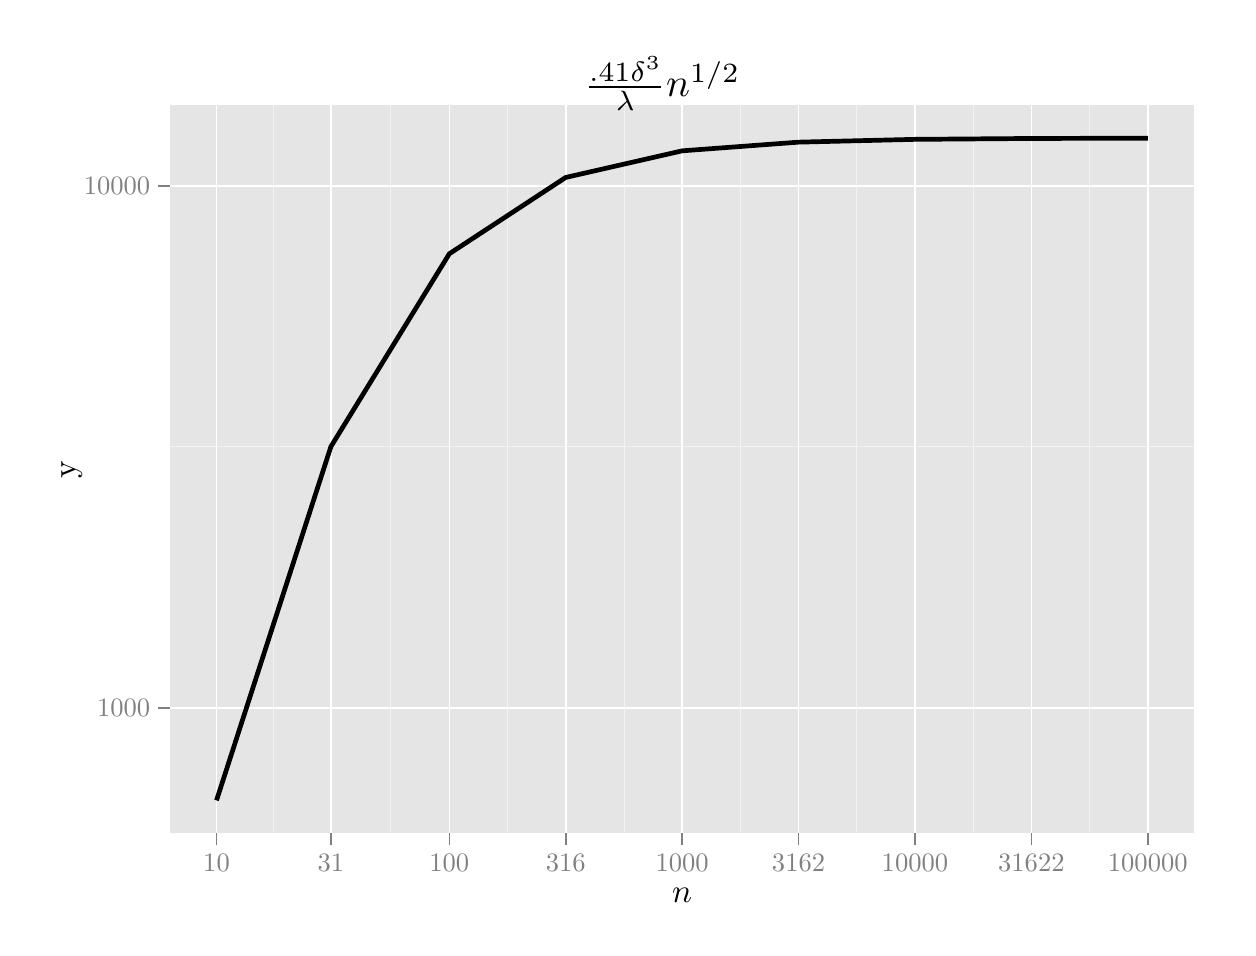
\begin{tikzpicture}[x=1pt,y=1pt]
\definecolor[named]{fillColor}{rgb}{1.00,1.00,1.00}
\path[use as bounding box,fill=fillColor,fill opacity=0.00] (0,0) rectangle (433.62,325.21);
\begin{scope}
\path[clip] (  0.00,  0.00) rectangle (433.62,325.21);
\definecolor[named]{drawColor}{rgb}{1.00,1.00,1.00}
\definecolor[named]{fillColor}{rgb}{1.00,1.00,1.00}

\path[draw=drawColor,line width= 0.6pt,line join=round,line cap=round,fill=fillColor] (  0.00,  0.00) rectangle (433.62,325.21);
\end{scope}
\begin{scope}
\path[clip] ( 51.42, 34.03) rectangle (421.57,297.23);
\definecolor[named]{fillColor}{rgb}{0.90,0.90,0.90}

\path[fill=fillColor] ( 51.42, 34.03) rectangle (421.57,297.23);
\definecolor[named]{drawColor}{rgb}{0.95,0.95,0.95}

\path[draw=drawColor,line width= 0.3pt,line join=round] ( 51.42,173.77) --
	(421.57,173.77);

\path[draw=drawColor,line width= 0.3pt,line join=round] ( 88.91, 34.03) --
	( 88.91,297.23);

\path[draw=drawColor,line width= 0.3pt,line join=round] (130.97, 34.03) --
	(130.97,297.23);

\path[draw=drawColor,line width= 0.3pt,line join=round] (173.39, 34.03) --
	(173.39,297.23);

\path[draw=drawColor,line width= 0.3pt,line join=round] (215.45, 34.03) --
	(215.45,297.23);

\path[draw=drawColor,line width= 0.3pt,line join=round] (257.53, 34.03) --
	(257.53,297.23);

\path[draw=drawColor,line width= 0.3pt,line join=round] (299.59, 34.03) --
	(299.59,297.23);

\path[draw=drawColor,line width= 0.3pt,line join=round] (341.65, 34.03) --
	(341.65,297.23);

\path[draw=drawColor,line width= 0.3pt,line join=round] (383.72, 34.03) --
	(383.72,297.23);
\definecolor[named]{drawColor}{rgb}{1.00,1.00,1.00}

\path[draw=drawColor,line width= 0.6pt,line join=round] ( 51.42, 79.46) --
	(421.57, 79.46);

\path[draw=drawColor,line width= 0.6pt,line join=round] ( 51.42,268.08) --
	(421.57,268.08);

\path[draw=drawColor,line width= 0.6pt,line join=round] ( 68.24, 34.03) --
	( 68.24,297.23);

\path[draw=drawColor,line width= 0.6pt,line join=round] (109.58, 34.03) --
	(109.58,297.23);

\path[draw=drawColor,line width= 0.6pt,line join=round] (152.37, 34.03) --
	(152.37,297.23);

\path[draw=drawColor,line width= 0.6pt,line join=round] (194.41, 34.03) --
	(194.41,297.23);

\path[draw=drawColor,line width= 0.6pt,line join=round] (236.50, 34.03) --
	(236.50,297.23);

\path[draw=drawColor,line width= 0.6pt,line join=round] (278.56, 34.03) --
	(278.56,297.23);

\path[draw=drawColor,line width= 0.6pt,line join=round] (320.62, 34.03) --
	(320.62,297.23);

\path[draw=drawColor,line width= 0.6pt,line join=round] (362.69, 34.03) --
	(362.69,297.23);

\path[draw=drawColor,line width= 0.6pt,line join=round] (404.75, 34.03) --
	(404.75,297.23);
\definecolor[named]{drawColor}{rgb}{0.00,0.00,0.00}

\path[draw=drawColor,line width= 1.7pt,line join=round] ( 68.24, 46.00) --
	(109.58,173.84) --
	(152.37,243.51) --
	(194.41,271.08) --
	(236.50,280.70) --
	(278.56,283.84) --
	(320.62,284.85) --
	(362.69,285.17) --
	(404.75,285.27);
\end{scope}
\begin{scope}
\path[clip] (  0.00,  0.00) rectangle (433.62,325.21);
\definecolor[named]{drawColor}{rgb}{0.50,0.50,0.50}

\node[text=drawColor,anchor=base east,inner sep=0pt, outer sep=0pt, scale=  0.96] at ( 44.30, 76.15) {1000};

\node[text=drawColor,anchor=base east,inner sep=0pt, outer sep=0pt, scale=  0.96] at ( 44.30,264.78) {10000};
\end{scope}
\begin{scope}
\path[clip] (  0.00,  0.00) rectangle (433.62,325.21);
\definecolor[named]{drawColor}{rgb}{0.50,0.50,0.50}

\path[draw=drawColor,line width= 0.6pt,line join=round] ( 47.15, 79.46) --
	( 51.42, 79.46);

\path[draw=drawColor,line width= 0.6pt,line join=round] ( 47.15,268.08) --
	( 51.42,268.08);
\end{scope}
\begin{scope}
\path[clip] (  0.00,  0.00) rectangle (433.62,325.21);
\definecolor[named]{drawColor}{rgb}{0.50,0.50,0.50}

\path[draw=drawColor,line width= 0.6pt,line join=round] ( 68.24, 29.77) --
	( 68.24, 34.03);

\path[draw=drawColor,line width= 0.6pt,line join=round] (109.58, 29.77) --
	(109.58, 34.03);

\path[draw=drawColor,line width= 0.6pt,line join=round] (152.37, 29.77) --
	(152.37, 34.03);

\path[draw=drawColor,line width= 0.6pt,line join=round] (194.41, 29.77) --
	(194.41, 34.03);

\path[draw=drawColor,line width= 0.6pt,line join=round] (236.50, 29.77) --
	(236.50, 34.03);

\path[draw=drawColor,line width= 0.6pt,line join=round] (278.56, 29.77) --
	(278.56, 34.03);

\path[draw=drawColor,line width= 0.6pt,line join=round] (320.62, 29.77) --
	(320.62, 34.03);

\path[draw=drawColor,line width= 0.6pt,line join=round] (362.69, 29.77) --
	(362.69, 34.03);

\path[draw=drawColor,line width= 0.6pt,line join=round] (404.75, 29.77) --
	(404.75, 34.03);
\end{scope}
\begin{scope}
\path[clip] (  0.00,  0.00) rectangle (433.62,325.21);
\definecolor[named]{drawColor}{rgb}{0.50,0.50,0.50}

\node[text=drawColor,anchor=base,inner sep=0pt, outer sep=0pt, scale=  0.96] at ( 68.24, 20.31) {10};

\node[text=drawColor,anchor=base,inner sep=0pt, outer sep=0pt, scale=  0.96] at (109.58, 20.31) {31};

\node[text=drawColor,anchor=base,inner sep=0pt, outer sep=0pt, scale=  0.96] at (152.37, 20.31) {100};

\node[text=drawColor,anchor=base,inner sep=0pt, outer sep=0pt, scale=  0.96] at (194.41, 20.31) {316};

\node[text=drawColor,anchor=base,inner sep=0pt, outer sep=0pt, scale=  0.96] at (236.50, 20.31) {1000};

\node[text=drawColor,anchor=base,inner sep=0pt, outer sep=0pt, scale=  0.96] at (278.56, 20.31) {3162};

\node[text=drawColor,anchor=base,inner sep=0pt, outer sep=0pt, scale=  0.96] at (320.62, 20.31) {10000};

\node[text=drawColor,anchor=base,inner sep=0pt, outer sep=0pt, scale=  0.96] at (362.69, 20.31) {31622};

\node[text=drawColor,anchor=base,inner sep=0pt, outer sep=0pt, scale=  0.96] at (404.75, 20.31) {100000};
\end{scope}
\begin{scope}
\path[clip] (  0.00,  0.00) rectangle (433.62,325.21);
\definecolor[named]{drawColor}{rgb}{0.00,0.00,0.00}

\node[text=drawColor,anchor=base,inner sep=0pt, outer sep=0pt, scale=  1.20] at (236.50,  9.03) {$n$};
\end{scope}
\begin{scope}
\path[clip] (  0.00,  0.00) rectangle (433.62,325.21);
\definecolor[named]{drawColor}{rgb}{0.00,0.00,0.00}

\node[text=drawColor,rotate= 90.00,anchor=base,inner sep=0pt, outer sep=0pt, scale=  1.20] at ( 17.30,165.63) {y};
\end{scope}
\begin{scope}
\path[clip] (  0.00,  0.00) rectangle (433.62,325.21);
\definecolor[named]{drawColor}{rgb}{0.00,0.00,0.00}

\node[text=drawColor,anchor=base,inner sep=0pt, outer sep=0pt, scale=  1.44] at (236.50,300.24) {$\frac{.41\delta^3}{\lambda}n^{1/2}\quad $};
\end{scope}
\end{tikzpicture}

    }
  \end{center}
\end{frame}

\begin{frame}{Twitter Example}
  \begin{figure}[!ht]
   \centering
   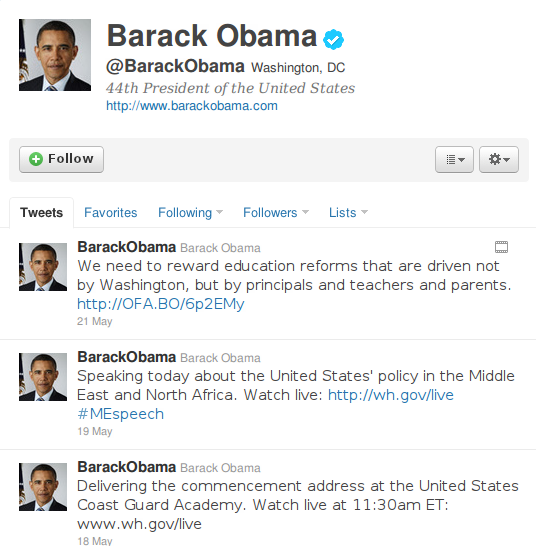
\includegraphics[scale=.3]{pres3.png}
   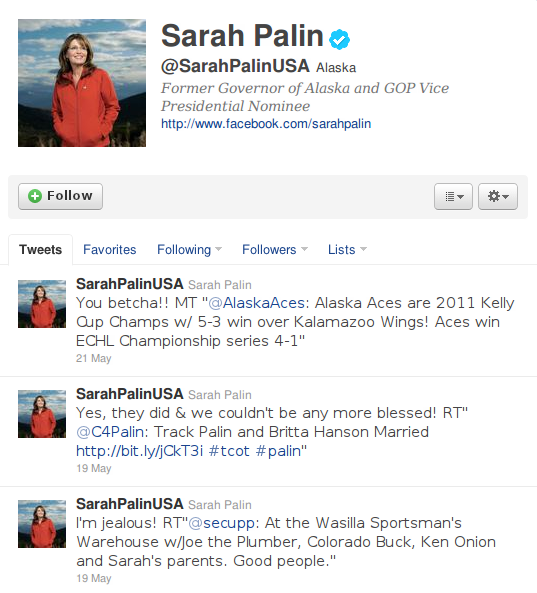
\includegraphics[scale=.3]{pres4.png}
 \end{figure}
\end{frame}

\begin{frame}[fragile]{Twitter Data}
  Raw:
\begin{verbatim}
"BarackObama: We need to reward education reforms that are
driven not by Washington, but by principals and teachers and
parents. http://OFA.BO/6p2EMy"
"SarahPalinUSA: You betcha!! MT \"@AlaskaAces: Alaska Aces
are 2011 Kelly Cup Champs w/ 5-3 win over Kalamazoo Wings!
Aces win  ECHL Championship series 4-1\""
\end{verbatim}
  After pre-processing:
\begin{verbatim}
"we need to reward education reforms that are driven not by
washington but by principals and teachers and parents "
"you betcha mt alaskaaces alaska aces are  kelly cup champs
w  win over kalamazoo wings aces win  echl championship
series "
\end{verbatim}
\end{frame}

\begin{frame}{The Spectrum Kernel}
  Compares two strings based on the their length $k$ contiguous
  subsequences. \pause
  \begin{itemize}
  \item $\mathcal{X}$ is our input space, built up from an alphabet
    $\mathcal{A} = \{a,b,\ldots,z,$ $\}$ with $|\mathcal{A}|=27$. \pause
  \item The $k$-spectrum ($k \geq 1$) of an input sequence is the set
    of all length $k$ contiguous subsequences it contains. \pause
  \item Define the feature map from $\mathcal{X}$ to
    $\mathbb{R}^{|\mathcal{A}|^k}$ by $\Phi_k(x) = (\phi_a(x))_{a \in
      \mathcal{A}^k}$ where $\phi_a(x)$ is the number of times $a$
    occurs in $x$: $\{\#aaa,\#aab,\#aac,\ldots,\}$. \pause
  \item $K_k(x,y) = \langle \Phi_k(x),\Phi_k(y) \rangle$.
  \end{itemize}
\end{frame}

\begin{frame}{Support Vector Machines for Regression}
Consider the $\ell_1$-regularized (soft-margin) support vector classification problem:
\begin{equation*}
\begin{aligned}
& \underset{\mathbf{w} \in \mathcal{H}, b \in \mathbb{R}}{\text{minimize}}
& &\frac{1}{2}\norm{\mathbf{w}}^2+C\sum_{i=1}^M \xi_i \\
& \text{subject to}
& & y_i(\mathbf{w}^t \mathbf{x}_i + b) \geq 1 - \xi_i \\
&&& \xi_i \geq 0 \qquad \qquad \quad \text{for all } i=1,\ldots,m.
\end{aligned}
\end{equation*}
For the Friedman Test, our scoring function is the margin
$f(\mathbf{x}_i) = \sum_{i=1}^m y_i \alpha_i k(\mathbf{x}, \mathbf{x}_i) + b$.
\end{frame}

\begin{frame}{Twitter Example}
  \begin{center}
    \resizebox{10.0cm}{!}{
      % Created by tikzDevice version 0.6.2-92-0ad2792 on 2013-03-31 12:28:06
% !TEX encoding = UTF-8 Unicode
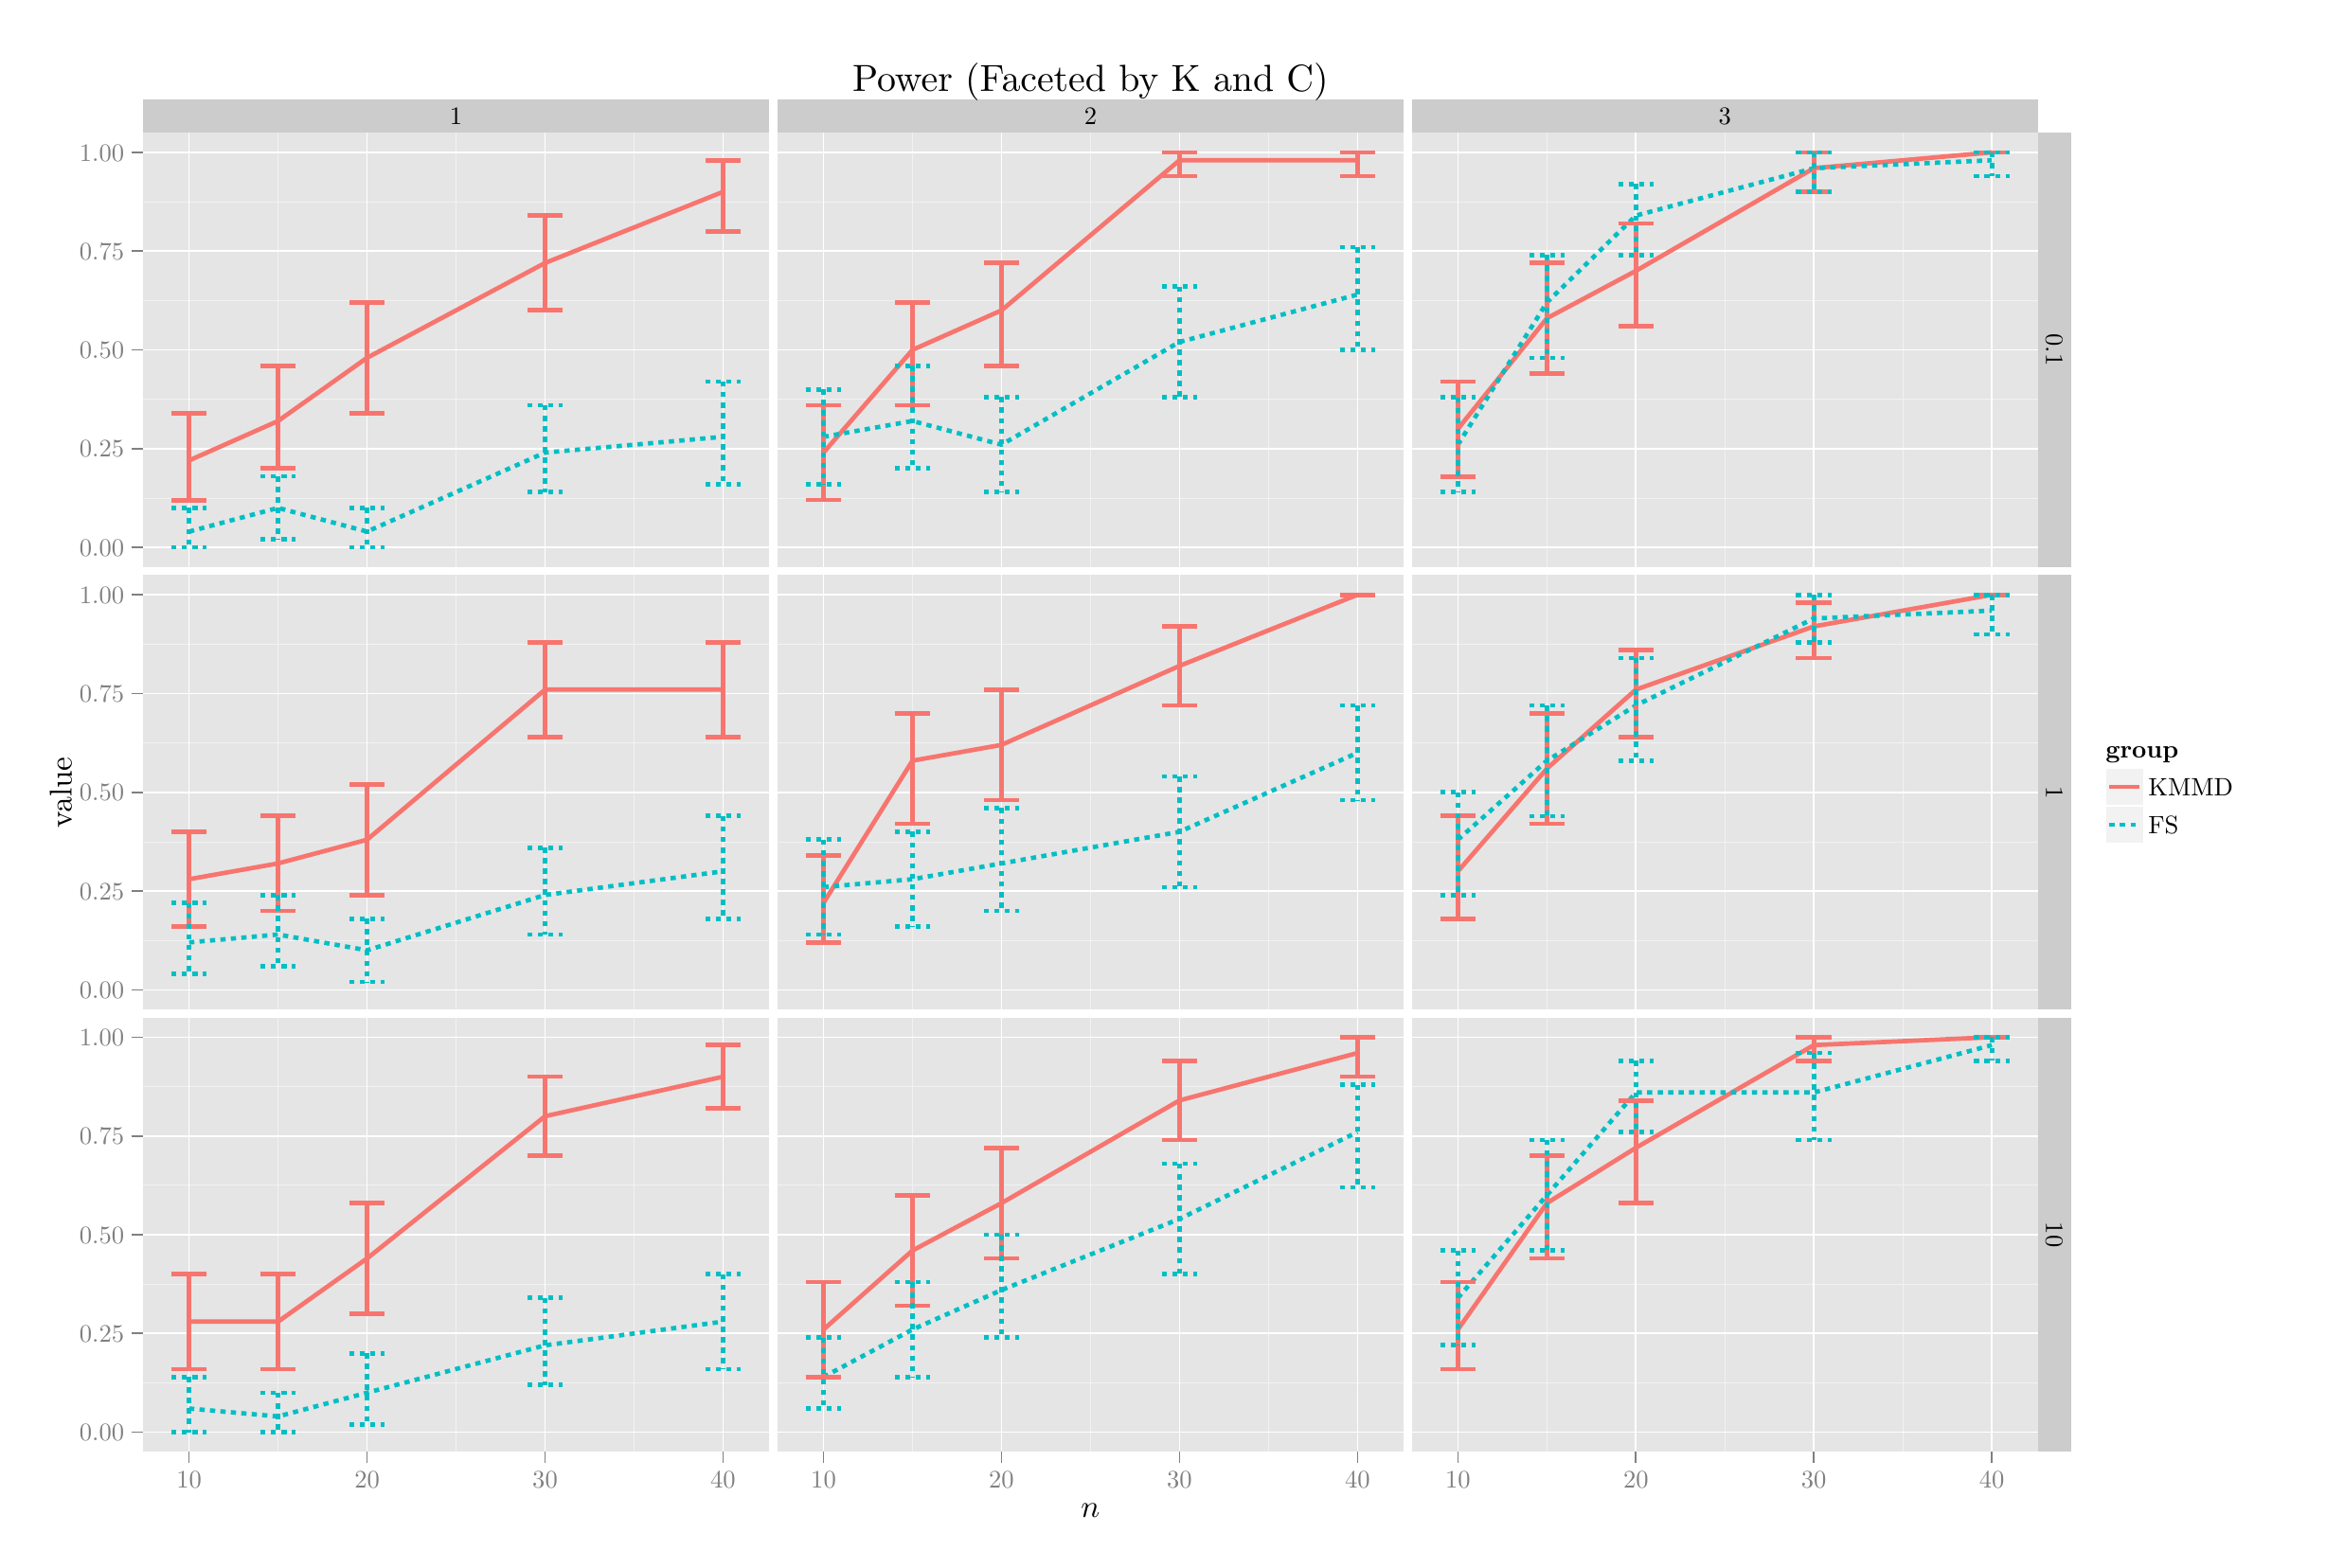
\begin{tikzpicture}[x=1pt,y=1pt]
\definecolor[named]{fillColor}{rgb}{1.00,1.00,1.00}
\path[use as bounding box,fill=fillColor,fill opacity=0.00] (0,0) rectangle (867.24,578.16);
\begin{scope}
\path[clip] (  0.00,  0.00) rectangle (867.24,578.16);
\definecolor[named]{drawColor}{rgb}{1.00,1.00,1.00}
\definecolor[named]{fillColor}{rgb}{1.00,1.00,1.00}

\path[draw=drawColor,line width= 0.6pt,line join=round,line cap=round,fill=fillColor] (  0.00, -0.00) rectangle (867.24,578.16);
\end{scope}
\begin{scope}
\path[clip] ( 44.49,537.54) rectangle (283.53,550.17);
\definecolor[named]{fillColor}{rgb}{0.80,0.80,0.80}

\path[fill=fillColor] ( 44.49,537.54) rectangle (283.53,550.17);
\definecolor[named]{drawColor}{rgb}{0.00,0.00,0.00}

\node[text=drawColor,anchor=base,inner sep=0pt, outer sep=0pt, scale=  0.96] at (164.01,540.55) {1};
\end{scope}
\begin{scope}
\path[clip] (286.54,537.54) rectangle (525.58,550.17);
\definecolor[named]{fillColor}{rgb}{0.80,0.80,0.80}

\path[fill=fillColor] (286.54,537.54) rectangle (525.58,550.17);
\definecolor[named]{drawColor}{rgb}{0.00,0.00,0.00}

\node[text=drawColor,anchor=base,inner sep=0pt, outer sep=0pt, scale=  0.96] at (406.06,540.55) {2};
\end{scope}
\begin{scope}
\path[clip] (528.59,537.54) rectangle (767.64,550.17);
\definecolor[named]{fillColor}{rgb}{0.80,0.80,0.80}

\path[fill=fillColor] (528.59,537.54) rectangle (767.64,550.17);
\definecolor[named]{drawColor}{rgb}{0.00,0.00,0.00}

\node[text=drawColor,anchor=base,inner sep=0pt, outer sep=0pt, scale=  0.96] at (648.11,540.55) {3};
\end{scope}
\begin{scope}
\path[clip] ( 44.49,371.71) rectangle (283.53,537.54);
\definecolor[named]{fillColor}{rgb}{0.90,0.90,0.90}

\path[fill=fillColor] ( 44.49,371.71) rectangle (283.53,537.54);
\definecolor[named]{drawColor}{rgb}{0.95,0.95,0.95}

\path[draw=drawColor,line width= 0.3pt,line join=round] ( 44.49,398.09) --
	(283.53,398.09);

\path[draw=drawColor,line width= 0.3pt,line join=round] ( 44.49,435.78) --
	(283.53,435.78);

\path[draw=drawColor,line width= 0.3pt,line join=round] ( 44.49,473.47) --
	(283.53,473.47);

\path[draw=drawColor,line width= 0.3pt,line join=round] ( 44.49,511.16) --
	(283.53,511.16);

\path[draw=drawColor,line width= 0.3pt,line join=round] ( 96.10,371.71) --
	( 96.10,537.54);

\path[draw=drawColor,line width= 0.3pt,line join=round] (164.01,371.71) --
	(164.01,537.54);

\path[draw=drawColor,line width= 0.3pt,line join=round] (231.92,371.71) --
	(231.92,537.54);
\definecolor[named]{drawColor}{rgb}{1.00,1.00,1.00}

\path[draw=drawColor,line width= 0.6pt,line join=round] ( 44.49,379.25) --
	(283.53,379.25);

\path[draw=drawColor,line width= 0.6pt,line join=round] ( 44.49,416.94) --
	(283.53,416.94);

\path[draw=drawColor,line width= 0.6pt,line join=round] ( 44.49,454.63) --
	(283.53,454.63);

\path[draw=drawColor,line width= 0.6pt,line join=round] ( 44.49,492.31) --
	(283.53,492.31);

\path[draw=drawColor,line width= 0.6pt,line join=round] ( 44.49,530.00) --
	(283.53,530.00);

\path[draw=drawColor,line width= 0.6pt,line join=round] ( 62.14,371.71) --
	( 62.14,537.54);

\path[draw=drawColor,line width= 0.6pt,line join=round] (130.05,371.71) --
	(130.05,537.54);

\path[draw=drawColor,line width= 0.6pt,line join=round] (197.96,371.71) --
	(197.96,537.54);

\path[draw=drawColor,line width= 0.6pt,line join=round] (265.87,371.71) --
	(265.87,537.54);
\definecolor[named]{drawColor}{rgb}{0.97,0.46,0.43}

\path[draw=drawColor,line width= 1.7pt,line join=round] ( 62.14,412.42) --
	( 96.10,427.49) --
	(130.05,451.61) --
	(197.96,487.79) --
	(265.87,514.93);
\definecolor[named]{drawColor}{rgb}{0.00,0.75,0.77}

\path[draw=drawColor,line width= 1.7pt,dash pattern=on 2pt off 2pt ,line join=round] ( 62.14,385.28) --
	( 96.10,394.33) --
	(130.05,385.28) --
	(197.96,415.43) --
	(265.87,421.46);
\definecolor[named]{drawColor}{rgb}{0.97,0.46,0.43}

\path[draw=drawColor,line width= 1.7pt,line join=round] ( 55.35,430.51) --
	( 68.93,430.51);

\path[draw=drawColor,line width= 1.7pt,line join=round] ( 62.14,430.51) --
	( 62.14,397.27);

\path[draw=drawColor,line width= 1.7pt,line join=round] ( 55.35,397.27) --
	( 68.93,397.27);

\path[draw=drawColor,line width= 1.7pt,line join=round] ( 89.31,448.60) --
	(102.89,448.60);

\path[draw=drawColor,line width= 1.7pt,line join=round] ( 96.10,448.60) --
	( 96.10,409.40);

\path[draw=drawColor,line width= 1.7pt,line join=round] ( 89.31,409.40) --
	(102.89,409.40);

\path[draw=drawColor,line width= 1.7pt,line join=round] (123.26,472.72) --
	(136.84,472.72);

\path[draw=drawColor,line width= 1.7pt,line join=round] (130.05,472.72) --
	(130.05,430.51);

\path[draw=drawColor,line width= 1.7pt,line join=round] (123.26,430.51) --
	(136.84,430.51);

\path[draw=drawColor,line width= 1.7pt,line join=round] (191.17,505.88) --
	(204.75,505.88);

\path[draw=drawColor,line width= 1.7pt,line join=round] (197.96,505.88) --
	(197.96,469.70);

\path[draw=drawColor,line width= 1.7pt,line join=round] (191.17,469.70) --
	(204.75,469.70);

\path[draw=drawColor,line width= 1.7pt,line join=round] (259.08,526.99) --
	(272.66,526.99);

\path[draw=drawColor,line width= 1.7pt,line join=round] (265.87,526.99) --
	(265.87,499.85);

\path[draw=drawColor,line width= 1.7pt,line join=round] (259.08,499.85) --
	(272.66,499.85);
\definecolor[named]{drawColor}{rgb}{0.00,0.75,0.77}

\path[draw=drawColor,line width= 1.7pt,dash pattern=on 2pt off 2pt ,line join=round] ( 55.35,394.33) --
	( 68.93,394.33);

\path[draw=drawColor,line width= 1.7pt,dash pattern=on 2pt off 2pt ,line join=round] ( 62.14,394.33) --
	( 62.14,379.25);

\path[draw=drawColor,line width= 1.7pt,dash pattern=on 2pt off 2pt ,line join=round] ( 55.35,379.25) --
	( 68.93,379.25);

\path[draw=drawColor,line width= 1.7pt,dash pattern=on 2pt off 2pt ,line join=round] ( 89.31,406.39) --
	(102.89,406.39);

\path[draw=drawColor,line width= 1.7pt,dash pattern=on 2pt off 2pt ,line join=round] ( 96.10,406.39) --
	( 96.10,382.27);

\path[draw=drawColor,line width= 1.7pt,dash pattern=on 2pt off 2pt ,line join=round] ( 89.31,382.27) --
	(102.89,382.27);

\path[draw=drawColor,line width= 1.7pt,dash pattern=on 2pt off 2pt ,line join=round] (123.26,394.33) --
	(136.84,394.33);

\path[draw=drawColor,line width= 1.7pt,dash pattern=on 2pt off 2pt ,line join=round] (130.05,394.33) --
	(130.05,379.25);

\path[draw=drawColor,line width= 1.7pt,dash pattern=on 2pt off 2pt ,line join=round] (123.26,379.25) --
	(136.84,379.25);

\path[draw=drawColor,line width= 1.7pt,dash pattern=on 2pt off 2pt ,line join=round] (191.17,433.52) --
	(204.75,433.52);

\path[draw=drawColor,line width= 1.7pt,dash pattern=on 2pt off 2pt ,line join=round] (197.96,433.52) --
	(197.96,400.36);

\path[draw=drawColor,line width= 1.7pt,dash pattern=on 2pt off 2pt ,line join=round] (191.17,400.36) --
	(204.75,400.36);

\path[draw=drawColor,line width= 1.7pt,dash pattern=on 2pt off 2pt ,line join=round] (259.08,442.57) --
	(272.66,442.57);

\path[draw=drawColor,line width= 1.7pt,dash pattern=on 2pt off 2pt ,line join=round] (265.87,442.57) --
	(265.87,403.37);

\path[draw=drawColor,line width= 1.7pt,dash pattern=on 2pt off 2pt ,line join=round] (259.08,403.37) --
	(272.66,403.37);
\end{scope}
\begin{scope}
\path[clip] ( 44.49,202.87) rectangle (283.53,368.70);
\definecolor[named]{fillColor}{rgb}{0.90,0.90,0.90}

\path[fill=fillColor] ( 44.49,202.87) rectangle (283.53,368.70);
\definecolor[named]{drawColor}{rgb}{0.95,0.95,0.95}

\path[draw=drawColor,line width= 0.3pt,line join=round] ( 44.49,229.26) --
	(283.53,229.26);

\path[draw=drawColor,line width= 0.3pt,line join=round] ( 44.49,266.94) --
	(283.53,266.94);

\path[draw=drawColor,line width= 0.3pt,line join=round] ( 44.49,304.63) --
	(283.53,304.63);

\path[draw=drawColor,line width= 0.3pt,line join=round] ( 44.49,342.32) --
	(283.53,342.32);

\path[draw=drawColor,line width= 0.3pt,line join=round] ( 96.10,202.87) --
	( 96.10,368.70);

\path[draw=drawColor,line width= 0.3pt,line join=round] (164.01,202.87) --
	(164.01,368.70);

\path[draw=drawColor,line width= 0.3pt,line join=round] (231.92,202.87) --
	(231.92,368.70);
\definecolor[named]{drawColor}{rgb}{1.00,1.00,1.00}

\path[draw=drawColor,line width= 0.6pt,line join=round] ( 44.49,210.41) --
	(283.53,210.41);

\path[draw=drawColor,line width= 0.6pt,line join=round] ( 44.49,248.10) --
	(283.53,248.10);

\path[draw=drawColor,line width= 0.6pt,line join=round] ( 44.49,285.79) --
	(283.53,285.79);

\path[draw=drawColor,line width= 0.6pt,line join=round] ( 44.49,323.48) --
	(283.53,323.48);

\path[draw=drawColor,line width= 0.6pt,line join=round] ( 44.49,361.16) --
	(283.53,361.16);

\path[draw=drawColor,line width= 0.6pt,line join=round] ( 62.14,202.87) --
	( 62.14,368.70);

\path[draw=drawColor,line width= 0.6pt,line join=round] (130.05,202.87) --
	(130.05,368.70);

\path[draw=drawColor,line width= 0.6pt,line join=round] (197.96,202.87) --
	(197.96,368.70);

\path[draw=drawColor,line width= 0.6pt,line join=round] (265.87,202.87) --
	(265.87,368.70);
\definecolor[named]{drawColor}{rgb}{0.97,0.46,0.43}

\path[draw=drawColor,line width= 1.7pt,line join=round] ( 62.14,252.62) --
	( 96.10,258.65) --
	(130.05,267.70) --
	(197.96,324.98) --
	(265.87,324.98);
\definecolor[named]{drawColor}{rgb}{0.00,0.75,0.77}

\path[draw=drawColor,line width= 1.7pt,dash pattern=on 2pt off 2pt ,line join=round] ( 62.14,228.50) --
	( 96.10,231.52) --
	(130.05,225.49) --
	(197.96,246.59) --
	(265.87,255.64);
\definecolor[named]{drawColor}{rgb}{0.97,0.46,0.43}

\path[draw=drawColor,line width= 1.7pt,line join=round] ( 55.35,270.71) --
	( 68.93,270.71);

\path[draw=drawColor,line width= 1.7pt,line join=round] ( 62.14,270.71) --
	( 62.14,234.53);

\path[draw=drawColor,line width= 1.7pt,line join=round] ( 55.35,234.53) --
	( 68.93,234.53);

\path[draw=drawColor,line width= 1.7pt,line join=round] ( 89.31,276.74) --
	(102.89,276.74);

\path[draw=drawColor,line width= 1.7pt,line join=round] ( 96.10,276.74) --
	( 96.10,240.56);

\path[draw=drawColor,line width= 1.7pt,line join=round] ( 89.31,240.56) --
	(102.89,240.56);

\path[draw=drawColor,line width= 1.7pt,line join=round] (123.26,288.80) --
	(136.84,288.80);

\path[draw=drawColor,line width= 1.7pt,line join=round] (130.05,288.80) --
	(130.05,246.59);

\path[draw=drawColor,line width= 1.7pt,line join=round] (123.26,246.59) --
	(136.84,246.59);

\path[draw=drawColor,line width= 1.7pt,line join=round] (191.17,343.07) --
	(204.75,343.07);

\path[draw=drawColor,line width= 1.7pt,line join=round] (197.96,343.07) --
	(197.96,306.89);

\path[draw=drawColor,line width= 1.7pt,line join=round] (191.17,306.89) --
	(204.75,306.89);

\path[draw=drawColor,line width= 1.7pt,line join=round] (259.08,343.07) --
	(272.66,343.07);

\path[draw=drawColor,line width= 1.7pt,line join=round] (265.87,343.07) --
	(265.87,306.89);

\path[draw=drawColor,line width= 1.7pt,line join=round] (259.08,306.89) --
	(272.66,306.89);
\definecolor[named]{drawColor}{rgb}{0.00,0.75,0.77}

\path[draw=drawColor,line width= 1.7pt,dash pattern=on 2pt off 2pt ,line join=round] ( 55.35,243.58) --
	( 68.93,243.58);

\path[draw=drawColor,line width= 1.7pt,dash pattern=on 2pt off 2pt ,line join=round] ( 62.14,243.58) --
	( 62.14,216.44);

\path[draw=drawColor,line width= 1.7pt,dash pattern=on 2pt off 2pt ,line join=round] ( 55.35,216.44) --
	( 68.93,216.44);

\path[draw=drawColor,line width= 1.7pt,dash pattern=on 2pt off 2pt ,line join=round] ( 89.31,246.59) --
	(102.89,246.59);

\path[draw=drawColor,line width= 1.7pt,dash pattern=on 2pt off 2pt ,line join=round] ( 96.10,246.59) --
	( 96.10,219.46);

\path[draw=drawColor,line width= 1.7pt,dash pattern=on 2pt off 2pt ,line join=round] ( 89.31,219.46) --
	(102.89,219.46);

\path[draw=drawColor,line width= 1.7pt,dash pattern=on 2pt off 2pt ,line join=round] (123.26,237.55) --
	(136.84,237.55);

\path[draw=drawColor,line width= 1.7pt,dash pattern=on 2pt off 2pt ,line join=round] (130.05,237.55) --
	(130.05,213.43);

\path[draw=drawColor,line width= 1.7pt,dash pattern=on 2pt off 2pt ,line join=round] (123.26,213.43) --
	(136.84,213.43);

\path[draw=drawColor,line width= 1.7pt,dash pattern=on 2pt off 2pt ,line join=round] (191.17,264.68) --
	(204.75,264.68);

\path[draw=drawColor,line width= 1.7pt,dash pattern=on 2pt off 2pt ,line join=round] (197.96,264.68) --
	(197.96,231.52);

\path[draw=drawColor,line width= 1.7pt,dash pattern=on 2pt off 2pt ,line join=round] (191.17,231.52) --
	(204.75,231.52);

\path[draw=drawColor,line width= 1.7pt,dash pattern=on 2pt off 2pt ,line join=round] (259.08,276.74) --
	(272.66,276.74);

\path[draw=drawColor,line width= 1.7pt,dash pattern=on 2pt off 2pt ,line join=round] (265.87,276.74) --
	(265.87,237.55);

\path[draw=drawColor,line width= 1.7pt,dash pattern=on 2pt off 2pt ,line join=round] (259.08,237.55) --
	(272.66,237.55);
\end{scope}
\begin{scope}
\path[clip] ( 44.49, 34.03) rectangle (283.53,199.86);
\definecolor[named]{fillColor}{rgb}{0.90,0.90,0.90}

\path[fill=fillColor] ( 44.49, 34.03) rectangle (283.53,199.86);
\definecolor[named]{drawColor}{rgb}{0.95,0.95,0.95}

\path[draw=drawColor,line width= 0.3pt,line join=round] ( 44.49, 60.42) --
	(283.53, 60.42);

\path[draw=drawColor,line width= 0.3pt,line join=round] ( 44.49, 98.10) --
	(283.53, 98.10);

\path[draw=drawColor,line width= 0.3pt,line join=round] ( 44.49,135.79) --
	(283.53,135.79);

\path[draw=drawColor,line width= 0.3pt,line join=round] ( 44.49,173.48) --
	(283.53,173.48);

\path[draw=drawColor,line width= 0.3pt,line join=round] ( 96.10, 34.03) --
	( 96.10,199.86);

\path[draw=drawColor,line width= 0.3pt,line join=round] (164.01, 34.03) --
	(164.01,199.86);

\path[draw=drawColor,line width= 0.3pt,line join=round] (231.92, 34.03) --
	(231.92,199.86);
\definecolor[named]{drawColor}{rgb}{1.00,1.00,1.00}

\path[draw=drawColor,line width= 0.6pt,line join=round] ( 44.49, 41.57) --
	(283.53, 41.57);

\path[draw=drawColor,line width= 0.6pt,line join=round] ( 44.49, 79.26) --
	(283.53, 79.26);

\path[draw=drawColor,line width= 0.6pt,line join=round] ( 44.49,116.95) --
	(283.53,116.95);

\path[draw=drawColor,line width= 0.6pt,line join=round] ( 44.49,154.64) --
	(283.53,154.64);

\path[draw=drawColor,line width= 0.6pt,line join=round] ( 44.49,192.32) --
	(283.53,192.32);

\path[draw=drawColor,line width= 0.6pt,line join=round] ( 62.14, 34.03) --
	( 62.14,199.86);

\path[draw=drawColor,line width= 0.6pt,line join=round] (130.05, 34.03) --
	(130.05,199.86);

\path[draw=drawColor,line width= 0.6pt,line join=round] (197.96, 34.03) --
	(197.96,199.86);

\path[draw=drawColor,line width= 0.6pt,line join=round] (265.87, 34.03) --
	(265.87,199.86);
\definecolor[named]{drawColor}{rgb}{0.97,0.46,0.43}

\path[draw=drawColor,line width= 1.7pt,line join=round] ( 62.14, 83.78) --
	( 96.10, 83.78) --
	(130.05,107.90) --
	(197.96,162.17) --
	(265.87,177.25);
\definecolor[named]{drawColor}{rgb}{0.00,0.75,0.77}

\path[draw=drawColor,line width= 1.7pt,dash pattern=on 2pt off 2pt ,line join=round] ( 62.14, 50.62) --
	( 96.10, 47.60) --
	(130.05, 56.65) --
	(197.96, 74.74) --
	(265.87, 83.78);
\definecolor[named]{drawColor}{rgb}{0.97,0.46,0.43}

\path[draw=drawColor,line width= 1.7pt,line join=round] ( 55.35,101.87) --
	( 68.93,101.87);

\path[draw=drawColor,line width= 1.7pt,line join=round] ( 62.14,101.87) --
	( 62.14, 65.69);

\path[draw=drawColor,line width= 1.7pt,line join=round] ( 55.35, 65.69) --
	( 68.93, 65.69);

\path[draw=drawColor,line width= 1.7pt,line join=round] ( 89.31,101.87) --
	(102.89,101.87);

\path[draw=drawColor,line width= 1.7pt,line join=round] ( 96.10,101.87) --
	( 96.10, 65.69);

\path[draw=drawColor,line width= 1.7pt,line join=round] ( 89.31, 65.69) --
	(102.89, 65.69);

\path[draw=drawColor,line width= 1.7pt,line join=round] (123.26,129.01) --
	(136.84,129.01);

\path[draw=drawColor,line width= 1.7pt,line join=round] (130.05,129.01) --
	(130.05, 86.80);

\path[draw=drawColor,line width= 1.7pt,line join=round] (123.26, 86.80) --
	(136.84, 86.80);

\path[draw=drawColor,line width= 1.7pt,line join=round] (191.17,177.25) --
	(204.75,177.25);

\path[draw=drawColor,line width= 1.7pt,line join=round] (197.96,177.25) --
	(197.96,147.10);

\path[draw=drawColor,line width= 1.7pt,line join=round] (191.17,147.10) --
	(204.75,147.10);

\path[draw=drawColor,line width= 1.7pt,line join=round] (259.08,189.31) --
	(272.66,189.31);

\path[draw=drawColor,line width= 1.7pt,line join=round] (265.87,189.31) --
	(265.87,165.19);

\path[draw=drawColor,line width= 1.7pt,line join=round] (259.08,165.19) --
	(272.66,165.19);
\definecolor[named]{drawColor}{rgb}{0.00,0.75,0.77}

\path[draw=drawColor,line width= 1.7pt,dash pattern=on 2pt off 2pt ,line join=round] ( 55.35, 62.68) --
	( 68.93, 62.68);

\path[draw=drawColor,line width= 1.7pt,dash pattern=on 2pt off 2pt ,line join=round] ( 62.14, 62.68) --
	( 62.14, 41.57);

\path[draw=drawColor,line width= 1.7pt,dash pattern=on 2pt off 2pt ,line join=round] ( 55.35, 41.57) --
	( 68.93, 41.57);

\path[draw=drawColor,line width= 1.7pt,dash pattern=on 2pt off 2pt ,line join=round] ( 89.31, 56.65) --
	(102.89, 56.65);

\path[draw=drawColor,line width= 1.7pt,dash pattern=on 2pt off 2pt ,line join=round] ( 96.10, 56.65) --
	( 96.10, 41.57);

\path[draw=drawColor,line width= 1.7pt,dash pattern=on 2pt off 2pt ,line join=round] ( 89.31, 41.57) --
	(102.89, 41.57);

\path[draw=drawColor,line width= 1.7pt,dash pattern=on 2pt off 2pt ,line join=round] (123.26, 71.72) --
	(136.84, 71.72);

\path[draw=drawColor,line width= 1.7pt,dash pattern=on 2pt off 2pt ,line join=round] (130.05, 71.72) --
	(130.05, 44.59);

\path[draw=drawColor,line width= 1.7pt,dash pattern=on 2pt off 2pt ,line join=round] (123.26, 44.59) --
	(136.84, 44.59);

\path[draw=drawColor,line width= 1.7pt,dash pattern=on 2pt off 2pt ,line join=round] (191.17, 92.83) --
	(204.75, 92.83);

\path[draw=drawColor,line width= 1.7pt,dash pattern=on 2pt off 2pt ,line join=round] (197.96, 92.83) --
	(197.96, 59.66);

\path[draw=drawColor,line width= 1.7pt,dash pattern=on 2pt off 2pt ,line join=round] (191.17, 59.66) --
	(204.75, 59.66);

\path[draw=drawColor,line width= 1.7pt,dash pattern=on 2pt off 2pt ,line join=round] (259.08,101.87) --
	(272.66,101.87);

\path[draw=drawColor,line width= 1.7pt,dash pattern=on 2pt off 2pt ,line join=round] (265.87,101.87) --
	(265.87, 65.69);

\path[draw=drawColor,line width= 1.7pt,dash pattern=on 2pt off 2pt ,line join=round] (259.08, 65.69) --
	(272.66, 65.69);
\end{scope}
\begin{scope}
\path[clip] (286.54,371.71) rectangle (525.58,537.54);
\definecolor[named]{fillColor}{rgb}{0.90,0.90,0.90}

\path[fill=fillColor] (286.54,371.71) rectangle (525.58,537.54);
\definecolor[named]{drawColor}{rgb}{0.95,0.95,0.95}

\path[draw=drawColor,line width= 0.3pt,line join=round] (286.54,398.09) --
	(525.58,398.09);

\path[draw=drawColor,line width= 0.3pt,line join=round] (286.54,435.78) --
	(525.58,435.78);

\path[draw=drawColor,line width= 0.3pt,line join=round] (286.54,473.47) --
	(525.58,473.47);

\path[draw=drawColor,line width= 0.3pt,line join=round] (286.54,511.16) --
	(525.58,511.16);

\path[draw=drawColor,line width= 0.3pt,line join=round] (338.15,371.71) --
	(338.15,537.54);

\path[draw=drawColor,line width= 0.3pt,line join=round] (406.06,371.71) --
	(406.06,537.54);

\path[draw=drawColor,line width= 0.3pt,line join=round] (473.97,371.71) --
	(473.97,537.54);
\definecolor[named]{drawColor}{rgb}{1.00,1.00,1.00}

\path[draw=drawColor,line width= 0.6pt,line join=round] (286.54,379.25) --
	(525.58,379.25);

\path[draw=drawColor,line width= 0.6pt,line join=round] (286.54,416.94) --
	(525.58,416.94);

\path[draw=drawColor,line width= 0.6pt,line join=round] (286.54,454.63) --
	(525.58,454.63);

\path[draw=drawColor,line width= 0.6pt,line join=round] (286.54,492.31) --
	(525.58,492.31);

\path[draw=drawColor,line width= 0.6pt,line join=round] (286.54,530.00) --
	(525.58,530.00);

\path[draw=drawColor,line width= 0.6pt,line join=round] (304.20,371.71) --
	(304.20,537.54);

\path[draw=drawColor,line width= 0.6pt,line join=round] (372.11,371.71) --
	(372.11,537.54);

\path[draw=drawColor,line width= 0.6pt,line join=round] (440.02,371.71) --
	(440.02,537.54);

\path[draw=drawColor,line width= 0.6pt,line join=round] (507.93,371.71) --
	(507.93,537.54);
\definecolor[named]{drawColor}{rgb}{0.97,0.46,0.43}

\path[draw=drawColor,line width= 1.7pt,line join=round] (304.20,415.43) --
	(338.15,454.63) --
	(372.11,469.70) --
	(440.02,526.99) --
	(507.93,526.99);
\definecolor[named]{drawColor}{rgb}{0.00,0.75,0.77}

\path[draw=drawColor,line width= 1.7pt,dash pattern=on 2pt off 2pt ,line join=round] (304.20,421.46) --
	(338.15,427.49) --
	(372.11,418.45) --
	(440.02,457.64) --
	(507.93,475.73);
\definecolor[named]{drawColor}{rgb}{0.97,0.46,0.43}

\path[draw=drawColor,line width= 1.7pt,line join=round] (297.41,433.52) --
	(310.99,433.52);

\path[draw=drawColor,line width= 1.7pt,line join=round] (304.20,433.52) --
	(304.20,397.34);

\path[draw=drawColor,line width= 1.7pt,line join=round] (297.41,397.34) --
	(310.99,397.34);

\path[draw=drawColor,line width= 1.7pt,line join=round] (331.36,472.72) --
	(344.94,472.72);

\path[draw=drawColor,line width= 1.7pt,line join=round] (338.15,472.72) --
	(338.15,433.52);

\path[draw=drawColor,line width= 1.7pt,line join=round] (331.36,433.52) --
	(344.94,433.52);

\path[draw=drawColor,line width= 1.7pt,line join=round] (365.31,487.79) --
	(378.90,487.79);

\path[draw=drawColor,line width= 1.7pt,line join=round] (372.11,487.79) --
	(372.11,448.60);

\path[draw=drawColor,line width= 1.7pt,line join=round] (365.31,448.60) --
	(378.90,448.60);

\path[draw=drawColor,line width= 1.7pt,line join=round] (433.22,530.00) --
	(446.81,530.00);

\path[draw=drawColor,line width= 1.7pt,line join=round] (440.02,530.00) --
	(440.02,520.96);

\path[draw=drawColor,line width= 1.7pt,line join=round] (433.22,520.96) --
	(446.81,520.96);

\path[draw=drawColor,line width= 1.7pt,line join=round] (501.13,530.00) --
	(514.72,530.00);

\path[draw=drawColor,line width= 1.7pt,line join=round] (507.93,530.00) --
	(507.93,520.96);

\path[draw=drawColor,line width= 1.7pt,line join=round] (501.13,520.96) --
	(514.72,520.96);
\definecolor[named]{drawColor}{rgb}{0.00,0.75,0.77}

\path[draw=drawColor,line width= 1.7pt,dash pattern=on 2pt off 2pt ,line join=round] (297.41,439.55) --
	(310.99,439.55);

\path[draw=drawColor,line width= 1.7pt,dash pattern=on 2pt off 2pt ,line join=round] (304.20,439.55) --
	(304.20,403.30);

\path[draw=drawColor,line width= 1.7pt,dash pattern=on 2pt off 2pt ,line join=round] (297.41,403.30) --
	(310.99,403.30);

\path[draw=drawColor,line width= 1.7pt,dash pattern=on 2pt off 2pt ,line join=round] (331.36,448.60) --
	(344.94,448.60);

\path[draw=drawColor,line width= 1.7pt,dash pattern=on 2pt off 2pt ,line join=round] (338.15,448.60) --
	(338.15,409.40);

\path[draw=drawColor,line width= 1.7pt,dash pattern=on 2pt off 2pt ,line join=round] (331.36,409.40) --
	(344.94,409.40);

\path[draw=drawColor,line width= 1.7pt,dash pattern=on 2pt off 2pt ,line join=round] (365.31,436.61) --
	(378.90,436.61);

\path[draw=drawColor,line width= 1.7pt,dash pattern=on 2pt off 2pt ,line join=round] (372.11,436.61) --
	(372.11,400.36);

\path[draw=drawColor,line width= 1.7pt,dash pattern=on 2pt off 2pt ,line join=round] (365.31,400.36) --
	(378.90,400.36);

\path[draw=drawColor,line width= 1.7pt,dash pattern=on 2pt off 2pt ,line join=round] (433.22,478.75) --
	(446.81,478.75);

\path[draw=drawColor,line width= 1.7pt,dash pattern=on 2pt off 2pt ,line join=round] (440.02,478.75) --
	(440.02,436.54);

\path[draw=drawColor,line width= 1.7pt,dash pattern=on 2pt off 2pt ,line join=round] (433.22,436.54) --
	(446.81,436.54);

\path[draw=drawColor,line width= 1.7pt,dash pattern=on 2pt off 2pt ,line join=round] (501.13,493.82) --
	(514.72,493.82);

\path[draw=drawColor,line width= 1.7pt,dash pattern=on 2pt off 2pt ,line join=round] (507.93,493.82) --
	(507.93,454.63);

\path[draw=drawColor,line width= 1.7pt,dash pattern=on 2pt off 2pt ,line join=round] (501.13,454.63) --
	(514.72,454.63);
\end{scope}
\begin{scope}
\path[clip] (286.54,202.87) rectangle (525.58,368.70);
\definecolor[named]{fillColor}{rgb}{0.90,0.90,0.90}

\path[fill=fillColor] (286.54,202.87) rectangle (525.58,368.70);
\definecolor[named]{drawColor}{rgb}{0.95,0.95,0.95}

\path[draw=drawColor,line width= 0.3pt,line join=round] (286.54,229.26) --
	(525.58,229.26);

\path[draw=drawColor,line width= 0.3pt,line join=round] (286.54,266.94) --
	(525.58,266.94);

\path[draw=drawColor,line width= 0.3pt,line join=round] (286.54,304.63) --
	(525.58,304.63);

\path[draw=drawColor,line width= 0.3pt,line join=round] (286.54,342.32) --
	(525.58,342.32);

\path[draw=drawColor,line width= 0.3pt,line join=round] (338.15,202.87) --
	(338.15,368.70);

\path[draw=drawColor,line width= 0.3pt,line join=round] (406.06,202.87) --
	(406.06,368.70);

\path[draw=drawColor,line width= 0.3pt,line join=round] (473.97,202.87) --
	(473.97,368.70);
\definecolor[named]{drawColor}{rgb}{1.00,1.00,1.00}

\path[draw=drawColor,line width= 0.6pt,line join=round] (286.54,210.41) --
	(525.58,210.41);

\path[draw=drawColor,line width= 0.6pt,line join=round] (286.54,248.10) --
	(525.58,248.10);

\path[draw=drawColor,line width= 0.6pt,line join=round] (286.54,285.79) --
	(525.58,285.79);

\path[draw=drawColor,line width= 0.6pt,line join=round] (286.54,323.48) --
	(525.58,323.48);

\path[draw=drawColor,line width= 0.6pt,line join=round] (286.54,361.16) --
	(525.58,361.16);

\path[draw=drawColor,line width= 0.6pt,line join=round] (304.20,202.87) --
	(304.20,368.70);

\path[draw=drawColor,line width= 0.6pt,line join=round] (372.11,202.87) --
	(372.11,368.70);

\path[draw=drawColor,line width= 0.6pt,line join=round] (440.02,202.87) --
	(440.02,368.70);

\path[draw=drawColor,line width= 0.6pt,line join=round] (507.93,202.87) --
	(507.93,368.70);
\definecolor[named]{drawColor}{rgb}{0.97,0.46,0.43}

\path[draw=drawColor,line width= 1.7pt,line join=round] (304.20,243.58) --
	(338.15,297.85) --
	(372.11,303.88) --
	(440.02,334.03) --
	(507.93,361.16);
\definecolor[named]{drawColor}{rgb}{0.00,0.75,0.77}

\path[draw=drawColor,line width= 1.7pt,dash pattern=on 2pt off 2pt ,line join=round] (304.20,249.61) --
	(338.15,252.62) --
	(372.11,258.65) --
	(440.02,270.71) --
	(507.93,300.86);
\definecolor[named]{drawColor}{rgb}{0.97,0.46,0.43}

\path[draw=drawColor,line width= 1.7pt,line join=round] (297.41,261.67) --
	(310.99,261.67);

\path[draw=drawColor,line width= 1.7pt,line join=round] (304.20,261.67) --
	(304.20,228.50);

\path[draw=drawColor,line width= 1.7pt,line join=round] (297.41,228.50) --
	(310.99,228.50);

\path[draw=drawColor,line width= 1.7pt,line join=round] (331.36,315.94) --
	(344.94,315.94);

\path[draw=drawColor,line width= 1.7pt,line join=round] (338.15,315.94) --
	(338.15,273.73);

\path[draw=drawColor,line width= 1.7pt,line join=round] (331.36,273.73) --
	(344.94,273.73);

\path[draw=drawColor,line width= 1.7pt,line join=round] (365.31,324.98) --
	(378.90,324.98);

\path[draw=drawColor,line width= 1.7pt,line join=round] (372.11,324.98) --
	(372.11,282.77);

\path[draw=drawColor,line width= 1.7pt,line join=round] (365.31,282.77) --
	(378.90,282.77);

\path[draw=drawColor,line width= 1.7pt,line join=round] (433.22,349.10) --
	(446.81,349.10);

\path[draw=drawColor,line width= 1.7pt,line join=round] (440.02,349.10) --
	(440.02,318.95);

\path[draw=drawColor,line width= 1.7pt,line join=round] (433.22,318.95) --
	(446.81,318.95);

\path[draw=drawColor,line width= 1.7pt,line join=round] (501.13,361.16) --
	(514.72,361.16);

\path[draw=drawColor,line width= 1.7pt,line join=round] (507.93,361.16) --
	(507.93,361.16);

\path[draw=drawColor,line width= 1.7pt,line join=round] (501.13,361.16) --
	(514.72,361.16);
\definecolor[named]{drawColor}{rgb}{0.00,0.75,0.77}

\path[draw=drawColor,line width= 1.7pt,dash pattern=on 2pt off 2pt ,line join=round] (297.41,267.70) --
	(310.99,267.70);

\path[draw=drawColor,line width= 1.7pt,dash pattern=on 2pt off 2pt ,line join=round] (304.20,267.70) --
	(304.20,231.52);

\path[draw=drawColor,line width= 1.7pt,dash pattern=on 2pt off 2pt ,line join=round] (297.41,231.52) --
	(310.99,231.52);

\path[draw=drawColor,line width= 1.7pt,dash pattern=on 2pt off 2pt ,line join=round] (331.36,270.71) --
	(344.94,270.71);

\path[draw=drawColor,line width= 1.7pt,dash pattern=on 2pt off 2pt ,line join=round] (338.15,270.71) --
	(338.15,234.53);

\path[draw=drawColor,line width= 1.7pt,dash pattern=on 2pt off 2pt ,line join=round] (331.36,234.53) --
	(344.94,234.53);

\path[draw=drawColor,line width= 1.7pt,dash pattern=on 2pt off 2pt ,line join=round] (365.31,279.76) --
	(378.90,279.76);

\path[draw=drawColor,line width= 1.7pt,dash pattern=on 2pt off 2pt ,line join=round] (372.11,279.76) --
	(372.11,240.56);

\path[draw=drawColor,line width= 1.7pt,dash pattern=on 2pt off 2pt ,line join=round] (365.31,240.56) --
	(378.90,240.56);

\path[draw=drawColor,line width= 1.7pt,dash pattern=on 2pt off 2pt ,line join=round] (433.22,291.82) --
	(446.81,291.82);

\path[draw=drawColor,line width= 1.7pt,dash pattern=on 2pt off 2pt ,line join=round] (440.02,291.82) --
	(440.02,249.61);

\path[draw=drawColor,line width= 1.7pt,dash pattern=on 2pt off 2pt ,line join=round] (433.22,249.61) --
	(446.81,249.61);

\path[draw=drawColor,line width= 1.7pt,dash pattern=on 2pt off 2pt ,line join=round] (501.13,318.95) --
	(514.72,318.95);

\path[draw=drawColor,line width= 1.7pt,dash pattern=on 2pt off 2pt ,line join=round] (507.93,318.95) --
	(507.93,282.77);

\path[draw=drawColor,line width= 1.7pt,dash pattern=on 2pt off 2pt ,line join=round] (501.13,282.77) --
	(514.72,282.77);
\end{scope}
\begin{scope}
\path[clip] (286.54, 34.03) rectangle (525.58,199.86);
\definecolor[named]{fillColor}{rgb}{0.90,0.90,0.90}

\path[fill=fillColor] (286.54, 34.03) rectangle (525.58,199.86);
\definecolor[named]{drawColor}{rgb}{0.95,0.95,0.95}

\path[draw=drawColor,line width= 0.3pt,line join=round] (286.54, 60.42) --
	(525.58, 60.42);

\path[draw=drawColor,line width= 0.3pt,line join=round] (286.54, 98.10) --
	(525.58, 98.10);

\path[draw=drawColor,line width= 0.3pt,line join=round] (286.54,135.79) --
	(525.58,135.79);

\path[draw=drawColor,line width= 0.3pt,line join=round] (286.54,173.48) --
	(525.58,173.48);

\path[draw=drawColor,line width= 0.3pt,line join=round] (338.15, 34.03) --
	(338.15,199.86);

\path[draw=drawColor,line width= 0.3pt,line join=round] (406.06, 34.03) --
	(406.06,199.86);

\path[draw=drawColor,line width= 0.3pt,line join=round] (473.97, 34.03) --
	(473.97,199.86);
\definecolor[named]{drawColor}{rgb}{1.00,1.00,1.00}

\path[draw=drawColor,line width= 0.6pt,line join=round] (286.54, 41.57) --
	(525.58, 41.57);

\path[draw=drawColor,line width= 0.6pt,line join=round] (286.54, 79.26) --
	(525.58, 79.26);

\path[draw=drawColor,line width= 0.6pt,line join=round] (286.54,116.95) --
	(525.58,116.95);

\path[draw=drawColor,line width= 0.6pt,line join=round] (286.54,154.64) --
	(525.58,154.64);

\path[draw=drawColor,line width= 0.6pt,line join=round] (286.54,192.32) --
	(525.58,192.32);

\path[draw=drawColor,line width= 0.6pt,line join=round] (304.20, 34.03) --
	(304.20,199.86);

\path[draw=drawColor,line width= 0.6pt,line join=round] (372.11, 34.03) --
	(372.11,199.86);

\path[draw=drawColor,line width= 0.6pt,line join=round] (440.02, 34.03) --
	(440.02,199.86);

\path[draw=drawColor,line width= 0.6pt,line join=round] (507.93, 34.03) --
	(507.93,199.86);
\definecolor[named]{drawColor}{rgb}{0.97,0.46,0.43}

\path[draw=drawColor,line width= 1.7pt,line join=round] (304.20, 80.77) --
	(338.15,110.92) --
	(372.11,129.01) --
	(440.02,168.20) --
	(507.93,186.29);
\definecolor[named]{drawColor}{rgb}{0.00,0.75,0.77}

\path[draw=drawColor,line width= 1.7pt,dash pattern=on 2pt off 2pt ,line join=round] (304.20, 62.68) --
	(338.15, 80.77) --
	(372.11, 95.84) --
	(440.02,122.98) --
	(507.93,156.14);
\definecolor[named]{drawColor}{rgb}{0.97,0.46,0.43}

\path[draw=drawColor,line width= 1.7pt,line join=round] (297.41, 98.86) --
	(310.99, 98.86);

\path[draw=drawColor,line width= 1.7pt,line join=round] (304.20, 98.86) --
	(304.20, 62.68);

\path[draw=drawColor,line width= 1.7pt,line join=round] (297.41, 62.68) --
	(310.99, 62.68);

\path[draw=drawColor,line width= 1.7pt,line join=round] (331.36,132.02) --
	(344.94,132.02);

\path[draw=drawColor,line width= 1.7pt,line join=round] (338.15,132.02) --
	(338.15, 89.81);

\path[draw=drawColor,line width= 1.7pt,line join=round] (331.36, 89.81) --
	(344.94, 89.81);

\path[draw=drawColor,line width= 1.7pt,line join=round] (365.31,150.11) --
	(378.90,150.11);

\path[draw=drawColor,line width= 1.7pt,line join=round] (372.11,150.11) --
	(372.11,107.90);

\path[draw=drawColor,line width= 1.7pt,line join=round] (365.31,107.90) --
	(378.90,107.90);

\path[draw=drawColor,line width= 1.7pt,line join=round] (433.22,183.28) --
	(446.81,183.28);

\path[draw=drawColor,line width= 1.7pt,line join=round] (440.02,183.28) --
	(440.02,153.05);

\path[draw=drawColor,line width= 1.7pt,line join=round] (433.22,153.05) --
	(446.81,153.05);

\path[draw=drawColor,line width= 1.7pt,line join=round] (501.13,192.32) --
	(514.72,192.32);

\path[draw=drawColor,line width= 1.7pt,line join=round] (507.93,192.32) --
	(507.93,177.25);

\path[draw=drawColor,line width= 1.7pt,line join=round] (501.13,177.25) --
	(514.72,177.25);
\definecolor[named]{drawColor}{rgb}{0.00,0.75,0.77}

\path[draw=drawColor,line width= 1.7pt,dash pattern=on 2pt off 2pt ,line join=round] (297.41, 77.75) --
	(310.99, 77.75);

\path[draw=drawColor,line width= 1.7pt,dash pattern=on 2pt off 2pt ,line join=round] (304.20, 77.75) --
	(304.20, 50.62);

\path[draw=drawColor,line width= 1.7pt,dash pattern=on 2pt off 2pt ,line join=round] (297.41, 50.62) --
	(310.99, 50.62);

\path[draw=drawColor,line width= 1.7pt,dash pattern=on 2pt off 2pt ,line join=round] (331.36, 98.86) --
	(344.94, 98.86);

\path[draw=drawColor,line width= 1.7pt,dash pattern=on 2pt off 2pt ,line join=round] (338.15, 98.86) --
	(338.15, 62.68);

\path[draw=drawColor,line width= 1.7pt,dash pattern=on 2pt off 2pt ,line join=round] (331.36, 62.68) --
	(344.94, 62.68);

\path[draw=drawColor,line width= 1.7pt,dash pattern=on 2pt off 2pt ,line join=round] (365.31,116.95) --
	(378.90,116.95);

\path[draw=drawColor,line width= 1.7pt,dash pattern=on 2pt off 2pt ,line join=round] (372.11,116.95) --
	(372.11, 77.75);

\path[draw=drawColor,line width= 1.7pt,dash pattern=on 2pt off 2pt ,line join=round] (365.31, 77.75) --
	(378.90, 77.75);

\path[draw=drawColor,line width= 1.7pt,dash pattern=on 2pt off 2pt ,line join=round] (433.22,144.08) --
	(446.81,144.08);

\path[draw=drawColor,line width= 1.7pt,dash pattern=on 2pt off 2pt ,line join=round] (440.02,144.08) --
	(440.02,101.87);

\path[draw=drawColor,line width= 1.7pt,dash pattern=on 2pt off 2pt ,line join=round] (433.22,101.87) --
	(446.81,101.87);

\path[draw=drawColor,line width= 1.7pt,dash pattern=on 2pt off 2pt ,line join=round] (501.13,174.23) --
	(514.72,174.23);

\path[draw=drawColor,line width= 1.7pt,dash pattern=on 2pt off 2pt ,line join=round] (507.93,174.23) --
	(507.93,135.04);

\path[draw=drawColor,line width= 1.7pt,dash pattern=on 2pt off 2pt ,line join=round] (501.13,135.04) --
	(514.72,135.04);
\end{scope}
\begin{scope}
\path[clip] (528.59,371.71) rectangle (767.64,537.54);
\definecolor[named]{fillColor}{rgb}{0.90,0.90,0.90}

\path[fill=fillColor] (528.59,371.71) rectangle (767.64,537.54);
\definecolor[named]{drawColor}{rgb}{0.95,0.95,0.95}

\path[draw=drawColor,line width= 0.3pt,line join=round] (528.59,398.09) --
	(767.64,398.09);

\path[draw=drawColor,line width= 0.3pt,line join=round] (528.59,435.78) --
	(767.64,435.78);

\path[draw=drawColor,line width= 0.3pt,line join=round] (528.59,473.47) --
	(767.64,473.47);

\path[draw=drawColor,line width= 0.3pt,line join=round] (528.59,511.16) --
	(767.64,511.16);

\path[draw=drawColor,line width= 0.3pt,line join=round] (580.21,371.71) --
	(580.21,537.54);

\path[draw=drawColor,line width= 0.3pt,line join=round] (648.11,371.71) --
	(648.11,537.54);

\path[draw=drawColor,line width= 0.3pt,line join=round] (716.02,371.71) --
	(716.02,537.54);
\definecolor[named]{drawColor}{rgb}{1.00,1.00,1.00}

\path[draw=drawColor,line width= 0.6pt,line join=round] (528.59,379.25) --
	(767.64,379.25);

\path[draw=drawColor,line width= 0.6pt,line join=round] (528.59,416.94) --
	(767.64,416.94);

\path[draw=drawColor,line width= 0.6pt,line join=round] (528.59,454.63) --
	(767.64,454.63);

\path[draw=drawColor,line width= 0.6pt,line join=round] (528.59,492.31) --
	(767.64,492.31);

\path[draw=drawColor,line width= 0.6pt,line join=round] (528.59,530.00) --
	(767.64,530.00);

\path[draw=drawColor,line width= 0.6pt,line join=round] (546.25,371.71) --
	(546.25,537.54);

\path[draw=drawColor,line width= 0.6pt,line join=round] (614.16,371.71) --
	(614.16,537.54);

\path[draw=drawColor,line width= 0.6pt,line join=round] (682.07,371.71) --
	(682.07,537.54);

\path[draw=drawColor,line width= 0.6pt,line join=round] (749.98,371.71) --
	(749.98,537.54);
\definecolor[named]{drawColor}{rgb}{0.97,0.46,0.43}

\path[draw=drawColor,line width= 1.7pt,line join=round] (546.25,424.48) --
	(580.21,466.69) --
	(614.16,484.78) --
	(682.07,523.97) --
	(749.98,530.00);
\definecolor[named]{drawColor}{rgb}{0.00,0.75,0.77}

\path[draw=drawColor,line width= 1.7pt,dash pattern=on 2pt off 2pt ,line join=round] (546.25,418.45) --
	(580.21,472.72) --
	(614.16,505.88) --
	(682.07,523.97) --
	(749.98,526.99);
\definecolor[named]{drawColor}{rgb}{0.97,0.46,0.43}

\path[draw=drawColor,line width= 1.7pt,line join=round] (539.46,442.57) --
	(553.04,442.57);

\path[draw=drawColor,line width= 1.7pt,line join=round] (546.25,442.57) --
	(546.25,406.31);

\path[draw=drawColor,line width= 1.7pt,line join=round] (539.46,406.31) --
	(553.04,406.31);

\path[draw=drawColor,line width= 1.7pt,line join=round] (573.41,487.79) --
	(587.00,487.79);

\path[draw=drawColor,line width= 1.7pt,line join=round] (580.21,487.79) --
	(580.21,445.58);

\path[draw=drawColor,line width= 1.7pt,line join=round] (573.41,445.58) --
	(587.00,445.58);

\path[draw=drawColor,line width= 1.7pt,line join=round] (607.37,502.87) --
	(620.95,502.87);

\path[draw=drawColor,line width= 1.7pt,line join=round] (614.16,502.87) --
	(614.16,463.67);

\path[draw=drawColor,line width= 1.7pt,line join=round] (607.37,463.67) --
	(620.95,463.67);

\path[draw=drawColor,line width= 1.7pt,line join=round] (675.28,530.00) --
	(688.86,530.00);

\path[draw=drawColor,line width= 1.7pt,line join=round] (682.07,530.00) --
	(682.07,514.93);

\path[draw=drawColor,line width= 1.7pt,line join=round] (675.28,514.93) --
	(688.86,514.93);

\path[draw=drawColor,line width= 1.7pt,line join=round] (743.19,530.00) --
	(756.77,530.00);

\path[draw=drawColor,line width= 1.7pt,line join=round] (749.98,530.00) --
	(749.98,530.00);

\path[draw=drawColor,line width= 1.7pt,line join=round] (743.19,530.00) --
	(756.77,530.00);
\definecolor[named]{drawColor}{rgb}{0.00,0.75,0.77}

\path[draw=drawColor,line width= 1.7pt,dash pattern=on 2pt off 2pt ,line join=round] (539.46,436.54) --
	(553.04,436.54);

\path[draw=drawColor,line width= 1.7pt,dash pattern=on 2pt off 2pt ,line join=round] (546.25,436.54) --
	(546.25,400.36);

\path[draw=drawColor,line width= 1.7pt,dash pattern=on 2pt off 2pt ,line join=round] (539.46,400.36) --
	(553.04,400.36);

\path[draw=drawColor,line width= 1.7pt,dash pattern=on 2pt off 2pt ,line join=round] (573.41,490.88) --
	(587.00,490.88);

\path[draw=drawColor,line width= 1.7pt,dash pattern=on 2pt off 2pt ,line join=round] (580.21,490.88) --
	(580.21,451.61);

\path[draw=drawColor,line width= 1.7pt,dash pattern=on 2pt off 2pt ,line join=round] (573.41,451.61) --
	(587.00,451.61);

\path[draw=drawColor,line width= 1.7pt,dash pattern=on 2pt off 2pt ,line join=round] (607.37,517.94) --
	(620.95,517.94);

\path[draw=drawColor,line width= 1.7pt,dash pattern=on 2pt off 2pt ,line join=round] (614.16,517.94) --
	(614.16,490.81);

\path[draw=drawColor,line width= 1.7pt,dash pattern=on 2pt off 2pt ,line join=round] (607.37,490.81) --
	(620.95,490.81);

\path[draw=drawColor,line width= 1.7pt,dash pattern=on 2pt off 2pt ,line join=round] (675.28,530.00) --
	(688.86,530.00);

\path[draw=drawColor,line width= 1.7pt,dash pattern=on 2pt off 2pt ,line join=round] (682.07,530.00) --
	(682.07,514.93);

\path[draw=drawColor,line width= 1.7pt,dash pattern=on 2pt off 2pt ,line join=round] (675.28,514.93) --
	(688.86,514.93);

\path[draw=drawColor,line width= 1.7pt,dash pattern=on 2pt off 2pt ,line join=round] (743.19,530.00) --
	(756.77,530.00);

\path[draw=drawColor,line width= 1.7pt,dash pattern=on 2pt off 2pt ,line join=round] (749.98,530.00) --
	(749.98,520.96);

\path[draw=drawColor,line width= 1.7pt,dash pattern=on 2pt off 2pt ,line join=round] (743.19,520.96) --
	(756.77,520.96);
\end{scope}
\begin{scope}
\path[clip] (528.59,202.87) rectangle (767.64,368.70);
\definecolor[named]{fillColor}{rgb}{0.90,0.90,0.90}

\path[fill=fillColor] (528.59,202.87) rectangle (767.64,368.70);
\definecolor[named]{drawColor}{rgb}{0.95,0.95,0.95}

\path[draw=drawColor,line width= 0.3pt,line join=round] (528.59,229.26) --
	(767.64,229.26);

\path[draw=drawColor,line width= 0.3pt,line join=round] (528.59,266.94) --
	(767.64,266.94);

\path[draw=drawColor,line width= 0.3pt,line join=round] (528.59,304.63) --
	(767.64,304.63);

\path[draw=drawColor,line width= 0.3pt,line join=round] (528.59,342.32) --
	(767.64,342.32);

\path[draw=drawColor,line width= 0.3pt,line join=round] (580.21,202.87) --
	(580.21,368.70);

\path[draw=drawColor,line width= 0.3pt,line join=round] (648.11,202.87) --
	(648.11,368.70);

\path[draw=drawColor,line width= 0.3pt,line join=round] (716.02,202.87) --
	(716.02,368.70);
\definecolor[named]{drawColor}{rgb}{1.00,1.00,1.00}

\path[draw=drawColor,line width= 0.6pt,line join=round] (528.59,210.41) --
	(767.64,210.41);

\path[draw=drawColor,line width= 0.6pt,line join=round] (528.59,248.10) --
	(767.64,248.10);

\path[draw=drawColor,line width= 0.6pt,line join=round] (528.59,285.79) --
	(767.64,285.79);

\path[draw=drawColor,line width= 0.6pt,line join=round] (528.59,323.48) --
	(767.64,323.48);

\path[draw=drawColor,line width= 0.6pt,line join=round] (528.59,361.16) --
	(767.64,361.16);

\path[draw=drawColor,line width= 0.6pt,line join=round] (546.25,202.87) --
	(546.25,368.70);

\path[draw=drawColor,line width= 0.6pt,line join=round] (614.16,202.87) --
	(614.16,368.70);

\path[draw=drawColor,line width= 0.6pt,line join=round] (682.07,202.87) --
	(682.07,368.70);

\path[draw=drawColor,line width= 0.6pt,line join=round] (749.98,202.87) --
	(749.98,368.70);
\definecolor[named]{drawColor}{rgb}{0.97,0.46,0.43}

\path[draw=drawColor,line width= 1.7pt,line join=round] (546.25,255.64) --
	(580.21,294.83) --
	(614.16,324.98) --
	(682.07,349.10) --
	(749.98,361.16);
\definecolor[named]{drawColor}{rgb}{0.00,0.75,0.77}

\path[draw=drawColor,line width= 1.7pt,dash pattern=on 2pt off 2pt ,line join=round] (546.25,267.70) --
	(580.21,297.85) --
	(614.16,318.95) --
	(682.07,352.12) --
	(749.98,355.13);
\definecolor[named]{drawColor}{rgb}{0.97,0.46,0.43}

\path[draw=drawColor,line width= 1.7pt,line join=round] (539.46,276.74) --
	(553.04,276.74);

\path[draw=drawColor,line width= 1.7pt,line join=round] (546.25,276.74) --
	(546.25,237.55);

\path[draw=drawColor,line width= 1.7pt,line join=round] (539.46,237.55) --
	(553.04,237.55);

\path[draw=drawColor,line width= 1.7pt,line join=round] (573.41,315.94) --
	(587.00,315.94);

\path[draw=drawColor,line width= 1.7pt,line join=round] (580.21,315.94) --
	(580.21,273.73);

\path[draw=drawColor,line width= 1.7pt,line join=round] (573.41,273.73) --
	(587.00,273.73);

\path[draw=drawColor,line width= 1.7pt,line join=round] (607.37,340.06) --
	(620.95,340.06);

\path[draw=drawColor,line width= 1.7pt,line join=round] (614.16,340.06) --
	(614.16,306.89);

\path[draw=drawColor,line width= 1.7pt,line join=round] (607.37,306.89) --
	(620.95,306.89);

\path[draw=drawColor,line width= 1.7pt,line join=round] (675.28,358.15) --
	(688.86,358.15);

\path[draw=drawColor,line width= 1.7pt,line join=round] (682.07,358.15) --
	(682.07,337.04);

\path[draw=drawColor,line width= 1.7pt,line join=round] (675.28,337.04) --
	(688.86,337.04);

\path[draw=drawColor,line width= 1.7pt,line join=round] (743.19,361.16) --
	(756.77,361.16);

\path[draw=drawColor,line width= 1.7pt,line join=round] (749.98,361.16) --
	(749.98,361.16);

\path[draw=drawColor,line width= 1.7pt,line join=round] (743.19,361.16) --
	(756.77,361.16);
\definecolor[named]{drawColor}{rgb}{0.00,0.75,0.77}

\path[draw=drawColor,line width= 1.7pt,dash pattern=on 2pt off 2pt ,line join=round] (539.46,285.79) --
	(553.04,285.79);

\path[draw=drawColor,line width= 1.7pt,dash pattern=on 2pt off 2pt ,line join=round] (546.25,285.79) --
	(546.25,246.59);

\path[draw=drawColor,line width= 1.7pt,dash pattern=on 2pt off 2pt ,line join=round] (539.46,246.59) --
	(553.04,246.59);

\path[draw=drawColor,line width= 1.7pt,dash pattern=on 2pt off 2pt ,line join=round] (573.41,318.95) --
	(587.00,318.95);

\path[draw=drawColor,line width= 1.7pt,dash pattern=on 2pt off 2pt ,line join=round] (580.21,318.95) --
	(580.21,276.67);

\path[draw=drawColor,line width= 1.7pt,dash pattern=on 2pt off 2pt ,line join=round] (573.41,276.67) --
	(587.00,276.67);

\path[draw=drawColor,line width= 1.7pt,dash pattern=on 2pt off 2pt ,line join=round] (607.37,337.04) --
	(620.95,337.04);

\path[draw=drawColor,line width= 1.7pt,dash pattern=on 2pt off 2pt ,line join=round] (614.16,337.04) --
	(614.16,297.85);

\path[draw=drawColor,line width= 1.7pt,dash pattern=on 2pt off 2pt ,line join=round] (607.37,297.85) --
	(620.95,297.85);

\path[draw=drawColor,line width= 1.7pt,dash pattern=on 2pt off 2pt ,line join=round] (675.28,361.16) --
	(688.86,361.16);

\path[draw=drawColor,line width= 1.7pt,dash pattern=on 2pt off 2pt ,line join=round] (682.07,361.16) --
	(682.07,343.07);

\path[draw=drawColor,line width= 1.7pt,dash pattern=on 2pt off 2pt ,line join=round] (675.28,343.07) --
	(688.86,343.07);

\path[draw=drawColor,line width= 1.7pt,dash pattern=on 2pt off 2pt ,line join=round] (743.19,361.16) --
	(756.77,361.16);

\path[draw=drawColor,line width= 1.7pt,dash pattern=on 2pt off 2pt ,line join=round] (749.98,361.16) --
	(749.98,346.09);

\path[draw=drawColor,line width= 1.7pt,dash pattern=on 2pt off 2pt ,line join=round] (743.19,346.09) --
	(756.77,346.09);
\end{scope}
\begin{scope}
\path[clip] (528.59, 34.03) rectangle (767.64,199.86);
\definecolor[named]{fillColor}{rgb}{0.90,0.90,0.90}

\path[fill=fillColor] (528.59, 34.03) rectangle (767.64,199.86);
\definecolor[named]{drawColor}{rgb}{0.95,0.95,0.95}

\path[draw=drawColor,line width= 0.3pt,line join=round] (528.59, 60.42) --
	(767.64, 60.42);

\path[draw=drawColor,line width= 0.3pt,line join=round] (528.59, 98.10) --
	(767.64, 98.10);

\path[draw=drawColor,line width= 0.3pt,line join=round] (528.59,135.79) --
	(767.64,135.79);

\path[draw=drawColor,line width= 0.3pt,line join=round] (528.59,173.48) --
	(767.64,173.48);

\path[draw=drawColor,line width= 0.3pt,line join=round] (580.21, 34.03) --
	(580.21,199.86);

\path[draw=drawColor,line width= 0.3pt,line join=round] (648.11, 34.03) --
	(648.11,199.86);

\path[draw=drawColor,line width= 0.3pt,line join=round] (716.02, 34.03) --
	(716.02,199.86);
\definecolor[named]{drawColor}{rgb}{1.00,1.00,1.00}

\path[draw=drawColor,line width= 0.6pt,line join=round] (528.59, 41.57) --
	(767.64, 41.57);

\path[draw=drawColor,line width= 0.6pt,line join=round] (528.59, 79.26) --
	(767.64, 79.26);

\path[draw=drawColor,line width= 0.6pt,line join=round] (528.59,116.95) --
	(767.64,116.95);

\path[draw=drawColor,line width= 0.6pt,line join=round] (528.59,154.64) --
	(767.64,154.64);

\path[draw=drawColor,line width= 0.6pt,line join=round] (528.59,192.32) --
	(767.64,192.32);

\path[draw=drawColor,line width= 0.6pt,line join=round] (546.25, 34.03) --
	(546.25,199.86);

\path[draw=drawColor,line width= 0.6pt,line join=round] (614.16, 34.03) --
	(614.16,199.86);

\path[draw=drawColor,line width= 0.6pt,line join=round] (682.07, 34.03) --
	(682.07,199.86);

\path[draw=drawColor,line width= 0.6pt,line join=round] (749.98, 34.03) --
	(749.98,199.86);
\definecolor[named]{drawColor}{rgb}{0.97,0.46,0.43}

\path[draw=drawColor,line width= 1.7pt,line join=round] (546.25, 80.77) --
	(580.21,129.01) --
	(614.16,150.11) --
	(682.07,189.31) --
	(749.98,192.32);
\definecolor[named]{drawColor}{rgb}{0.00,0.75,0.77}

\path[draw=drawColor,line width= 1.7pt,dash pattern=on 2pt off 2pt ,line join=round] (546.25, 92.83) --
	(580.21,132.02) --
	(614.16,171.22) --
	(682.07,171.22) --
	(749.98,189.31);
\definecolor[named]{drawColor}{rgb}{0.97,0.46,0.43}

\path[draw=drawColor,line width= 1.7pt,line join=round] (539.46, 98.86) --
	(553.04, 98.86);

\path[draw=drawColor,line width= 1.7pt,line join=round] (546.25, 98.86) --
	(546.25, 65.62);

\path[draw=drawColor,line width= 1.7pt,line join=round] (539.46, 65.62) --
	(553.04, 65.62);

\path[draw=drawColor,line width= 1.7pt,line join=round] (573.41,147.10) --
	(587.00,147.10);

\path[draw=drawColor,line width= 1.7pt,line join=round] (580.21,147.10) --
	(580.21,107.90);

\path[draw=drawColor,line width= 1.7pt,line join=round] (573.41,107.90) --
	(587.00,107.90);

\path[draw=drawColor,line width= 1.7pt,line join=round] (607.37,168.20) --
	(620.95,168.20);

\path[draw=drawColor,line width= 1.7pt,line join=round] (614.16,168.20) --
	(614.16,129.01);

\path[draw=drawColor,line width= 1.7pt,line join=round] (607.37,129.01) --
	(620.95,129.01);

\path[draw=drawColor,line width= 1.7pt,line join=round] (675.28,192.32) --
	(688.86,192.32);

\path[draw=drawColor,line width= 1.7pt,line join=round] (682.07,192.32) --
	(682.07,183.28);

\path[draw=drawColor,line width= 1.7pt,line join=round] (675.28,183.28) --
	(688.86,183.28);

\path[draw=drawColor,line width= 1.7pt,line join=round] (743.19,192.32) --
	(756.77,192.32);

\path[draw=drawColor,line width= 1.7pt,line join=round] (749.98,192.32) --
	(749.98,192.32);

\path[draw=drawColor,line width= 1.7pt,line join=round] (743.19,192.32) --
	(756.77,192.32);
\definecolor[named]{drawColor}{rgb}{0.00,0.75,0.77}

\path[draw=drawColor,line width= 1.7pt,dash pattern=on 2pt off 2pt ,line join=round] (539.46,110.92) --
	(553.04,110.92);

\path[draw=drawColor,line width= 1.7pt,dash pattern=on 2pt off 2pt ,line join=round] (546.25,110.92) --
	(546.25, 74.74);

\path[draw=drawColor,line width= 1.7pt,dash pattern=on 2pt off 2pt ,line join=round] (539.46, 74.74) --
	(553.04, 74.74);

\path[draw=drawColor,line width= 1.7pt,dash pattern=on 2pt off 2pt ,line join=round] (573.41,153.13) --
	(587.00,153.13);

\path[draw=drawColor,line width= 1.7pt,dash pattern=on 2pt off 2pt ,line join=round] (580.21,153.13) --
	(580.21,110.92);

\path[draw=drawColor,line width= 1.7pt,dash pattern=on 2pt off 2pt ,line join=round] (573.41,110.92) --
	(587.00,110.92);

\path[draw=drawColor,line width= 1.7pt,dash pattern=on 2pt off 2pt ,line join=round] (607.37,183.28) --
	(620.95,183.28);

\path[draw=drawColor,line width= 1.7pt,dash pattern=on 2pt off 2pt ,line join=round] (614.16,183.28) --
	(614.16,156.14);

\path[draw=drawColor,line width= 1.7pt,dash pattern=on 2pt off 2pt ,line join=round] (607.37,156.14) --
	(620.95,156.14);

\path[draw=drawColor,line width= 1.7pt,dash pattern=on 2pt off 2pt ,line join=round] (675.28,186.29) --
	(688.86,186.29);

\path[draw=drawColor,line width= 1.7pt,dash pattern=on 2pt off 2pt ,line join=round] (682.07,186.29) --
	(682.07,153.13);

\path[draw=drawColor,line width= 1.7pt,dash pattern=on 2pt off 2pt ,line join=round] (675.28,153.13) --
	(688.86,153.13);

\path[draw=drawColor,line width= 1.7pt,dash pattern=on 2pt off 2pt ,line join=round] (743.19,192.32) --
	(756.77,192.32);

\path[draw=drawColor,line width= 1.7pt,dash pattern=on 2pt off 2pt ,line join=round] (749.98,192.32) --
	(749.98,183.28);

\path[draw=drawColor,line width= 1.7pt,dash pattern=on 2pt off 2pt ,line join=round] (743.19,183.28) --
	(756.77,183.28);
\end{scope}
\begin{scope}
\path[clip] (  0.00,  0.00) rectangle (867.24,578.16);
\definecolor[named]{drawColor}{rgb}{0.50,0.50,0.50}

\node[text=drawColor,anchor=base east,inner sep=0pt, outer sep=0pt, scale=  0.96] at ( 37.37,375.94) {0.00};

\node[text=drawColor,anchor=base east,inner sep=0pt, outer sep=0pt, scale=  0.96] at ( 37.37,413.63) {0.25};

\node[text=drawColor,anchor=base east,inner sep=0pt, outer sep=0pt, scale=  0.96] at ( 37.37,451.32) {0.50};

\node[text=drawColor,anchor=base east,inner sep=0pt, outer sep=0pt, scale=  0.96] at ( 37.37,489.01) {0.75};

\node[text=drawColor,anchor=base east,inner sep=0pt, outer sep=0pt, scale=  0.96] at ( 37.37,526.70) {1.00};
\end{scope}
\begin{scope}
\path[clip] (  0.00,  0.00) rectangle (867.24,578.16);
\definecolor[named]{drawColor}{rgb}{0.50,0.50,0.50}

\path[draw=drawColor,line width= 0.6pt,line join=round] ( 40.22,379.25) --
	( 44.49,379.25);

\path[draw=drawColor,line width= 0.6pt,line join=round] ( 40.22,416.94) --
	( 44.49,416.94);

\path[draw=drawColor,line width= 0.6pt,line join=round] ( 40.22,454.63) --
	( 44.49,454.63);

\path[draw=drawColor,line width= 0.6pt,line join=round] ( 40.22,492.31) --
	( 44.49,492.31);

\path[draw=drawColor,line width= 0.6pt,line join=round] ( 40.22,530.00) --
	( 44.49,530.00);
\end{scope}
\begin{scope}
\path[clip] (  0.00,  0.00) rectangle (867.24,578.16);
\definecolor[named]{drawColor}{rgb}{0.50,0.50,0.50}

\node[text=drawColor,anchor=base east,inner sep=0pt, outer sep=0pt, scale=  0.96] at ( 37.37,207.11) {0.00};

\node[text=drawColor,anchor=base east,inner sep=0pt, outer sep=0pt, scale=  0.96] at ( 37.37,244.79) {0.25};

\node[text=drawColor,anchor=base east,inner sep=0pt, outer sep=0pt, scale=  0.96] at ( 37.37,282.48) {0.50};

\node[text=drawColor,anchor=base east,inner sep=0pt, outer sep=0pt, scale=  0.96] at ( 37.37,320.17) {0.75};

\node[text=drawColor,anchor=base east,inner sep=0pt, outer sep=0pt, scale=  0.96] at ( 37.37,357.86) {1.00};
\end{scope}
\begin{scope}
\path[clip] (  0.00,  0.00) rectangle (867.24,578.16);
\definecolor[named]{drawColor}{rgb}{0.50,0.50,0.50}

\path[draw=drawColor,line width= 0.6pt,line join=round] ( 40.22,210.41) --
	( 44.49,210.41);

\path[draw=drawColor,line width= 0.6pt,line join=round] ( 40.22,248.10) --
	( 44.49,248.10);

\path[draw=drawColor,line width= 0.6pt,line join=round] ( 40.22,285.79) --
	( 44.49,285.79);

\path[draw=drawColor,line width= 0.6pt,line join=round] ( 40.22,323.48) --
	( 44.49,323.48);

\path[draw=drawColor,line width= 0.6pt,line join=round] ( 40.22,361.16) --
	( 44.49,361.16);
\end{scope}
\begin{scope}
\path[clip] (  0.00,  0.00) rectangle (867.24,578.16);
\definecolor[named]{drawColor}{rgb}{0.50,0.50,0.50}

\node[text=drawColor,anchor=base east,inner sep=0pt, outer sep=0pt, scale=  0.96] at ( 37.37, 38.27) {0.00};

\node[text=drawColor,anchor=base east,inner sep=0pt, outer sep=0pt, scale=  0.96] at ( 37.37, 75.95) {0.25};

\node[text=drawColor,anchor=base east,inner sep=0pt, outer sep=0pt, scale=  0.96] at ( 37.37,113.64) {0.50};

\node[text=drawColor,anchor=base east,inner sep=0pt, outer sep=0pt, scale=  0.96] at ( 37.37,151.33) {0.75};

\node[text=drawColor,anchor=base east,inner sep=0pt, outer sep=0pt, scale=  0.96] at ( 37.37,189.02) {1.00};
\end{scope}
\begin{scope}
\path[clip] (  0.00,  0.00) rectangle (867.24,578.16);
\definecolor[named]{drawColor}{rgb}{0.50,0.50,0.50}

\path[draw=drawColor,line width= 0.6pt,line join=round] ( 40.22, 41.57) --
	( 44.49, 41.57);

\path[draw=drawColor,line width= 0.6pt,line join=round] ( 40.22, 79.26) --
	( 44.49, 79.26);

\path[draw=drawColor,line width= 0.6pt,line join=round] ( 40.22,116.95) --
	( 44.49,116.95);

\path[draw=drawColor,line width= 0.6pt,line join=round] ( 40.22,154.64) --
	( 44.49,154.64);

\path[draw=drawColor,line width= 0.6pt,line join=round] ( 40.22,192.32) --
	( 44.49,192.32);
\end{scope}
\begin{scope}
\path[clip] (767.64,371.71) rectangle (780.27,537.54);
\definecolor[named]{fillColor}{rgb}{0.80,0.80,0.80}

\path[fill=fillColor] (767.64,371.71) rectangle (780.27,537.54);
\definecolor[named]{drawColor}{rgb}{0.00,0.00,0.00}

\node[text=drawColor,rotate=270.00,anchor=base,inner sep=0pt, outer sep=0pt, scale=  0.96] at (770.65,454.63) {0.1};
\end{scope}
\begin{scope}
\path[clip] (767.64,202.87) rectangle (780.27,368.70);
\definecolor[named]{fillColor}{rgb}{0.80,0.80,0.80}

\path[fill=fillColor] (767.64,202.87) rectangle (780.27,368.70);
\definecolor[named]{drawColor}{rgb}{0.00,0.00,0.00}

\node[text=drawColor,rotate=270.00,anchor=base,inner sep=0pt, outer sep=0pt, scale=  0.96] at (770.65,285.79) {1};
\end{scope}
\begin{scope}
\path[clip] (767.64, 34.03) rectangle (780.27,199.86);
\definecolor[named]{fillColor}{rgb}{0.80,0.80,0.80}

\path[fill=fillColor] (767.64, 34.03) rectangle (780.27,199.86);
\definecolor[named]{drawColor}{rgb}{0.00,0.00,0.00}

\node[text=drawColor,rotate=270.00,anchor=base,inner sep=0pt, outer sep=0pt, scale=  0.96] at (770.65,116.95) {10};
\end{scope}
\begin{scope}
\path[clip] (  0.00,  0.00) rectangle (867.24,578.16);
\definecolor[named]{drawColor}{rgb}{0.50,0.50,0.50}

\path[draw=drawColor,line width= 0.6pt,line join=round] ( 62.14, 29.77) --
	( 62.14, 34.03);

\path[draw=drawColor,line width= 0.6pt,line join=round] (130.05, 29.77) --
	(130.05, 34.03);

\path[draw=drawColor,line width= 0.6pt,line join=round] (197.96, 29.77) --
	(197.96, 34.03);

\path[draw=drawColor,line width= 0.6pt,line join=round] (265.87, 29.77) --
	(265.87, 34.03);
\end{scope}
\begin{scope}
\path[clip] (  0.00,  0.00) rectangle (867.24,578.16);
\definecolor[named]{drawColor}{rgb}{0.50,0.50,0.50}

\node[text=drawColor,anchor=base,inner sep=0pt, outer sep=0pt, scale=  0.96] at ( 62.14, 20.31) {10};

\node[text=drawColor,anchor=base,inner sep=0pt, outer sep=0pt, scale=  0.96] at (130.05, 20.31) {20};

\node[text=drawColor,anchor=base,inner sep=0pt, outer sep=0pt, scale=  0.96] at (197.96, 20.31) {30};

\node[text=drawColor,anchor=base,inner sep=0pt, outer sep=0pt, scale=  0.96] at (265.87, 20.31) {40};
\end{scope}
\begin{scope}
\path[clip] (  0.00,  0.00) rectangle (867.24,578.16);
\definecolor[named]{drawColor}{rgb}{0.50,0.50,0.50}

\path[draw=drawColor,line width= 0.6pt,line join=round] (304.20, 29.77) --
	(304.20, 34.03);

\path[draw=drawColor,line width= 0.6pt,line join=round] (372.11, 29.77) --
	(372.11, 34.03);

\path[draw=drawColor,line width= 0.6pt,line join=round] (440.02, 29.77) --
	(440.02, 34.03);

\path[draw=drawColor,line width= 0.6pt,line join=round] (507.93, 29.77) --
	(507.93, 34.03);
\end{scope}
\begin{scope}
\path[clip] (  0.00,  0.00) rectangle (867.24,578.16);
\definecolor[named]{drawColor}{rgb}{0.50,0.50,0.50}

\node[text=drawColor,anchor=base,inner sep=0pt, outer sep=0pt, scale=  0.96] at (304.20, 20.31) {10};

\node[text=drawColor,anchor=base,inner sep=0pt, outer sep=0pt, scale=  0.96] at (372.11, 20.31) {20};

\node[text=drawColor,anchor=base,inner sep=0pt, outer sep=0pt, scale=  0.96] at (440.02, 20.31) {30};

\node[text=drawColor,anchor=base,inner sep=0pt, outer sep=0pt, scale=  0.96] at (507.93, 20.31) {40};
\end{scope}
\begin{scope}
\path[clip] (  0.00,  0.00) rectangle (867.24,578.16);
\definecolor[named]{drawColor}{rgb}{0.50,0.50,0.50}

\path[draw=drawColor,line width= 0.6pt,line join=round] (546.25, 29.77) --
	(546.25, 34.03);

\path[draw=drawColor,line width= 0.6pt,line join=round] (614.16, 29.77) --
	(614.16, 34.03);

\path[draw=drawColor,line width= 0.6pt,line join=round] (682.07, 29.77) --
	(682.07, 34.03);

\path[draw=drawColor,line width= 0.6pt,line join=round] (749.98, 29.77) --
	(749.98, 34.03);
\end{scope}
\begin{scope}
\path[clip] (  0.00,  0.00) rectangle (867.24,578.16);
\definecolor[named]{drawColor}{rgb}{0.50,0.50,0.50}

\node[text=drawColor,anchor=base,inner sep=0pt, outer sep=0pt, scale=  0.96] at (546.25, 20.31) {10};

\node[text=drawColor,anchor=base,inner sep=0pt, outer sep=0pt, scale=  0.96] at (614.16, 20.31) {20};

\node[text=drawColor,anchor=base,inner sep=0pt, outer sep=0pt, scale=  0.96] at (682.07, 20.31) {30};

\node[text=drawColor,anchor=base,inner sep=0pt, outer sep=0pt, scale=  0.96] at (749.98, 20.31) {40};
\end{scope}
\begin{scope}
\path[clip] (  0.00,  0.00) rectangle (867.24,578.16);
\definecolor[named]{drawColor}{rgb}{0.00,0.00,0.00}

\node[text=drawColor,anchor=base,inner sep=0pt, outer sep=0pt, scale=  1.20] at (406.06,  9.03) {$n$};
\end{scope}
\begin{scope}
\path[clip] (  0.00,  0.00) rectangle (867.24,578.16);
\definecolor[named]{drawColor}{rgb}{0.00,0.00,0.00}

\node[text=drawColor,rotate= 90.00,anchor=base,inner sep=0pt, outer sep=0pt, scale=  1.20] at ( 17.30,285.79) {value};
\end{scope}
\begin{scope}
\path[clip] (  0.00,  0.00) rectangle (867.24,578.16);
\definecolor[named]{fillColor}{rgb}{1.00,1.00,1.00}

\path[fill=fillColor] (789.14,261.95) rectangle (846.33,309.63);
\end{scope}
\begin{scope}
\path[clip] (  0.00,  0.00) rectangle (867.24,578.16);
\definecolor[named]{drawColor}{rgb}{0.00,0.00,0.00}

\node[text=drawColor,anchor=base west,inner sep=0pt, outer sep=0pt, scale=  0.96] at (793.41,298.74) {\bfseries group};
\end{scope}
\begin{scope}
\path[clip] (  0.00,  0.00) rectangle (867.24,578.16);
\definecolor[named]{drawColor}{rgb}{1.00,1.00,1.00}
\definecolor[named]{fillColor}{rgb}{0.95,0.95,0.95}

\path[draw=drawColor,line width= 0.6pt,line join=round,line cap=round,fill=fillColor] (793.41,280.67) rectangle (807.86,295.12);
\end{scope}
\begin{scope}
\path[clip] (  0.00,  0.00) rectangle (867.24,578.16);
\definecolor[named]{drawColor}{rgb}{0.97,0.46,0.43}

\path[draw=drawColor,line width= 1.7pt,line join=round] (794.85,287.90) -- (806.41,287.90);
\end{scope}
\begin{scope}
\path[clip] (  0.00,  0.00) rectangle (867.24,578.16);
\definecolor[named]{drawColor}{rgb}{0.97,0.46,0.43}

\path[draw=drawColor,line width= 1.7pt,line join=round] (794.85,287.90) -- (806.41,287.90);
\end{scope}
\begin{scope}
\path[clip] (  0.00,  0.00) rectangle (867.24,578.16);
\definecolor[named]{drawColor}{rgb}{1.00,1.00,1.00}
\definecolor[named]{fillColor}{rgb}{0.95,0.95,0.95}

\path[draw=drawColor,line width= 0.6pt,line join=round,line cap=round,fill=fillColor] (793.41,266.21) rectangle (807.86,280.67);
\end{scope}
\begin{scope}
\path[clip] (  0.00,  0.00) rectangle (867.24,578.16);
\definecolor[named]{drawColor}{rgb}{0.00,0.75,0.77}

\path[draw=drawColor,line width= 1.7pt,dash pattern=on 2pt off 2pt ,line join=round] (794.85,273.44) -- (806.41,273.44);
\end{scope}
\begin{scope}
\path[clip] (  0.00,  0.00) rectangle (867.24,578.16);
\definecolor[named]{drawColor}{rgb}{0.00,0.75,0.77}

\path[draw=drawColor,line width= 1.7pt,dash pattern=on 2pt off 2pt ,line join=round] (794.85,273.44) -- (806.41,273.44);
\end{scope}
\begin{scope}
\path[clip] (  0.00,  0.00) rectangle (867.24,578.16);
\definecolor[named]{drawColor}{rgb}{0.00,0.00,0.00}

\node[text=drawColor,anchor=base west,inner sep=0pt, outer sep=0pt, scale=  0.96] at (809.67,284.59) {KMMD};
\end{scope}
\begin{scope}
\path[clip] (  0.00,  0.00) rectangle (867.24,578.16);
\definecolor[named]{drawColor}{rgb}{0.00,0.00,0.00}

\node[text=drawColor,anchor=base west,inner sep=0pt, outer sep=0pt, scale=  0.96] at (809.67,270.14) {FS};
\end{scope}
\begin{scope}
\path[clip] (  0.00,  0.00) rectangle (867.24,578.16);
\definecolor[named]{drawColor}{rgb}{0.00,0.00,0.00}

\node[text=drawColor,anchor=base,inner sep=0pt, outer sep=0pt, scale=  1.44] at (406.06,553.19) {Power (Faceted by K and C)};
\end{scope}
\end{tikzpicture}

    }
  \end{center}
\end{frame}

\begin{frame}{Image Data (Roosters)}
  Caltech 101 Object Categories \cite{fei2007learning} ($297 \times
  300$ grayscale)
  \begin{figure}
    \centering
    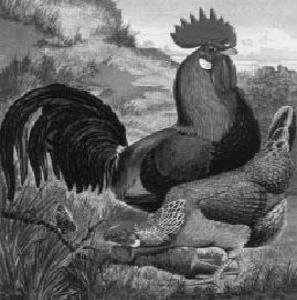
\includegraphics[scale=.35]{roosterrs-image_0001.jpg}
    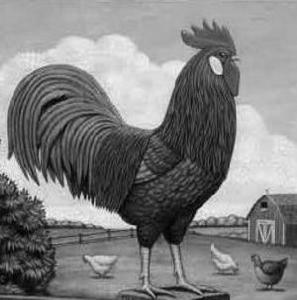
\includegraphics[scale=.35]{roosterrs-image_0002.jpg} \\
    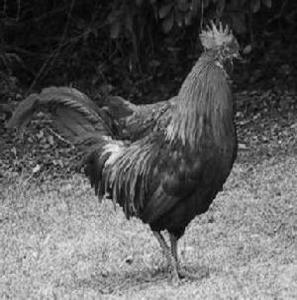
\includegraphics[scale=.35]{roosterrs-image_0003.jpg}
    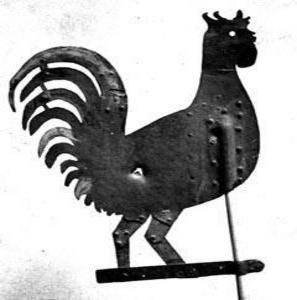
\includegraphics[scale=.35]{roosterrs-image_0004.jpg}
  \end{figure}
\end{frame}

\begin{frame}{Image Data (Pigeons)}
  \begin{figure}
    \centering
    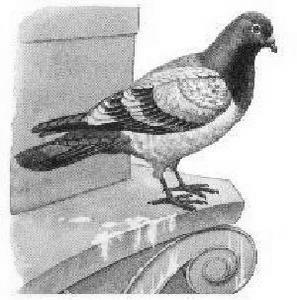
\includegraphics[scale=.35]{pigeonrs-image_0001.jpg}
    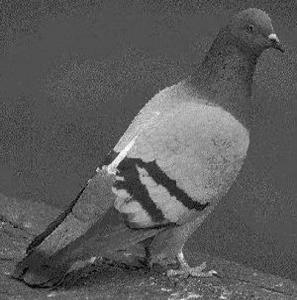
\includegraphics[scale=.35]{pigeonrs-image_0002.jpg} \\
    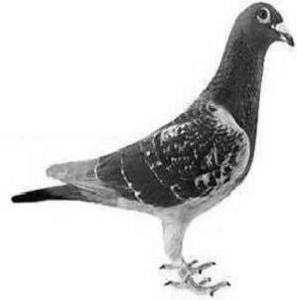
\includegraphics[scale=.35]{pigeonrs-image_0003.jpg}
    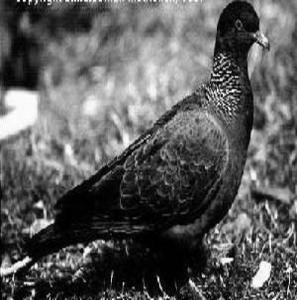
\includegraphics[scale=.35]{pigeonrs-image_0004.jpg}
  \end{figure}
\end{frame}

\begin{frame}{Polynomial Kernel}
  Each $m \times n$ grayscale image is converted to a vector of
  length $p=mn$.  \pause
  Given $X \in \mathbb{R}^{n \times p}$, the linear kernel is given by
  $$
  K(x, x') = \langle x, x'\rangle = \langle \Phi(x), \Phi(x')\rangle.
  $$
  The kernel matrix is given simply by $XX^T  \succeq 0$.  This
  corresponds to the identity mapping: $\Phi(x) = x$. \pause

  The homogeneous polynomial kernel,
  $$
  K(x, x') = \langle \Phi(x), \Phi(x')\rangle = \langle x, x' \rangle^d,
  $$
  corresponds to the mapping $\Phi(x) = [x_1^d, \ldots, x_p^d,
  x_1^{d-1}x_2, \ldots, x_p^{d-1}x_{p-1}]^T \in \mathbb{R}^{d'},
  \text{ where } d'=\binom{d+N-1}{d}$.
\end{frame}

\begin{frame}{Rooster/Pigeon Example}
  \begin{center}
    \resizebox{10.0cm}{!}{
      % Created by tikzDevice version 0.6.2-92-0ad2792 on 2013-03-06 14:04:27
% !TEX encoding = UTF-8 Unicode
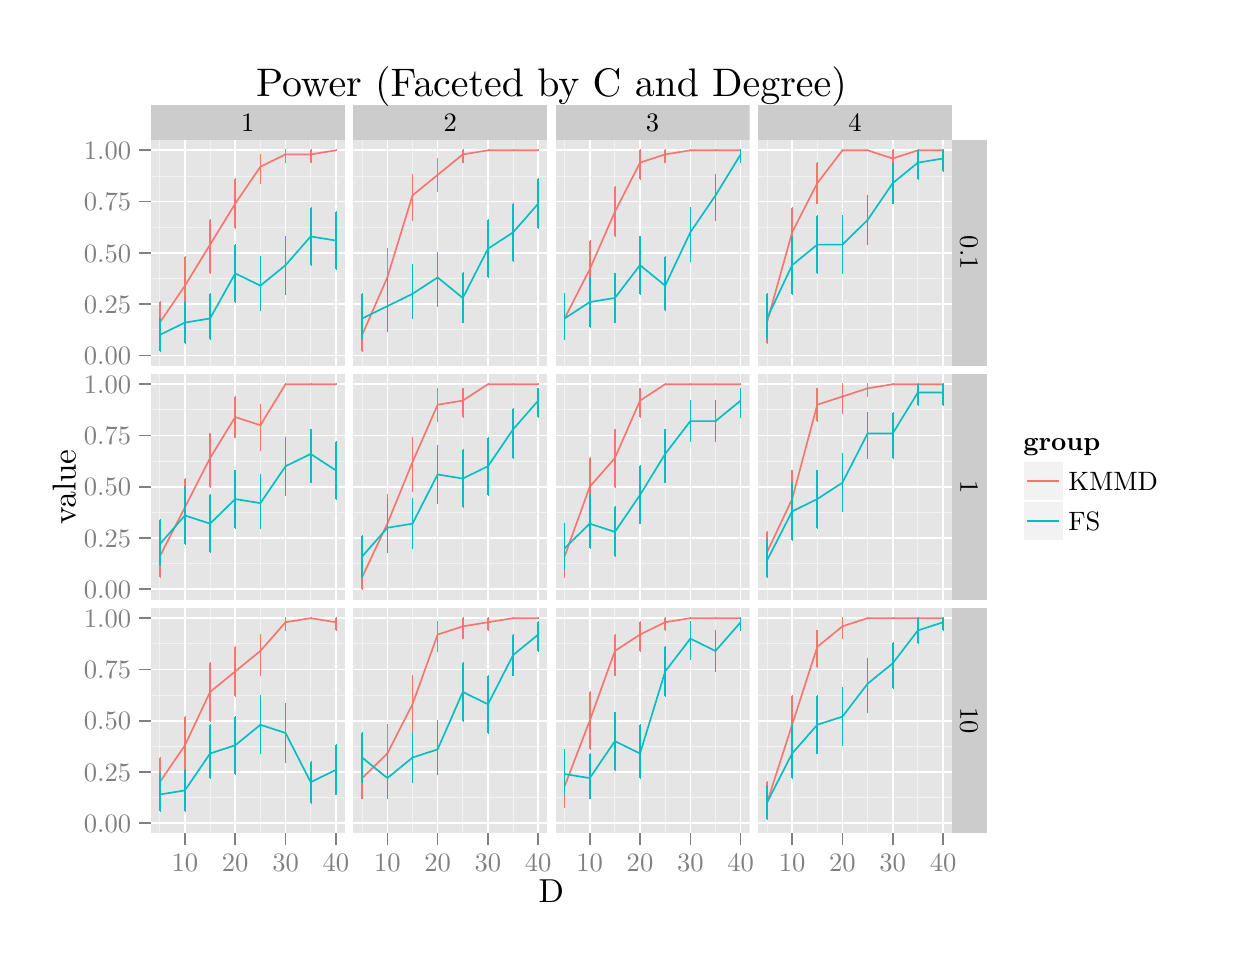
\begin{tikzpicture}[x=1pt,y=1pt]
\definecolor[named]{fillColor}{rgb}{1.00,1.00,1.00}
\path[use as bounding box,fill=fillColor,fill opacity=0.00] (0,0) rectangle (433.62,325.21);
\begin{scope}
\path[clip] (  0.00,  0.00) rectangle (433.62,325.21);
\definecolor[named]{drawColor}{rgb}{1.00,1.00,1.00}
\definecolor[named]{fillColor}{rgb}{1.00,1.00,1.00}

\path[draw=drawColor,line width= 0.6pt,line join=round,line cap=round,fill=fillColor] (  0.00,  0.00) rectangle (433.62,325.21);
\end{scope}
\begin{scope}
\path[clip] ( 44.49,284.60) rectangle (114.61,297.23);
\definecolor[named]{fillColor}{rgb}{0.80,0.80,0.80}

\path[fill=fillColor] ( 44.49,284.60) rectangle (114.61,297.23);
\definecolor[named]{drawColor}{rgb}{0.00,0.00,0.00}

\node[text=drawColor,anchor=base,inner sep=0pt, outer sep=0pt, scale=  0.96] at ( 79.55,287.61) {1};
\end{scope}
\begin{scope}
\path[clip] (117.62,284.60) rectangle (187.75,297.23);
\definecolor[named]{fillColor}{rgb}{0.80,0.80,0.80}

\path[fill=fillColor] (117.62,284.60) rectangle (187.75,297.23);
\definecolor[named]{drawColor}{rgb}{0.00,0.00,0.00}

\node[text=drawColor,anchor=base,inner sep=0pt, outer sep=0pt, scale=  0.96] at (152.68,287.61) {2};
\end{scope}
\begin{scope}
\path[clip] (190.76,284.60) rectangle (260.88,297.23);
\definecolor[named]{fillColor}{rgb}{0.80,0.80,0.80}

\path[fill=fillColor] (190.76,284.60) rectangle (260.88,297.23);
\definecolor[named]{drawColor}{rgb}{0.00,0.00,0.00}

\node[text=drawColor,anchor=base,inner sep=0pt, outer sep=0pt, scale=  0.96] at (225.82,287.61) {3};
\end{scope}
\begin{scope}
\path[clip] (263.89,284.60) rectangle (334.02,297.23);
\definecolor[named]{fillColor}{rgb}{0.80,0.80,0.80}

\path[fill=fillColor] (263.89,284.60) rectangle (334.02,297.23);
\definecolor[named]{drawColor}{rgb}{0.00,0.00,0.00}

\node[text=drawColor,anchor=base,inner sep=0pt, outer sep=0pt, scale=  0.96] at (298.95,287.61) {4};
\end{scope}
\begin{scope}
\path[clip] ( 44.49,203.08) rectangle (114.61,284.60);
\definecolor[named]{fillColor}{rgb}{0.90,0.90,0.90}

\path[fill=fillColor] ( 44.49,203.08) rectangle (114.61,284.60);
\definecolor[named]{drawColor}{rgb}{0.95,0.95,0.95}

\path[draw=drawColor,line width= 0.3pt,line join=round] ( 44.49,216.05) --
	(114.61,216.05);

\path[draw=drawColor,line width= 0.3pt,line join=round] ( 44.49,234.58) --
	(114.61,234.58);

\path[draw=drawColor,line width= 0.3pt,line join=round] ( 44.49,253.10) --
	(114.61,253.10);

\path[draw=drawColor,line width= 0.3pt,line join=round] ( 44.49,271.63) --
	(114.61,271.63);

\path[draw=drawColor,line width= 0.3pt,line join=round] ( 47.74,203.08) --
	( 47.74,284.60);

\path[draw=drawColor,line width= 0.3pt,line join=round] ( 65.91,203.08) --
	( 65.91,284.60);

\path[draw=drawColor,line width= 0.3pt,line join=round] ( 84.09,203.08) --
	( 84.09,284.60);

\path[draw=drawColor,line width= 0.3pt,line join=round] (102.27,203.08) --
	(102.27,284.60);
\definecolor[named]{drawColor}{rgb}{1.00,1.00,1.00}

\path[draw=drawColor,line width= 0.6pt,line join=round] ( 44.49,206.79) --
	(114.61,206.79);

\path[draw=drawColor,line width= 0.6pt,line join=round] ( 44.49,225.31) --
	(114.61,225.31);

\path[draw=drawColor,line width= 0.6pt,line join=round] ( 44.49,243.84) --
	(114.61,243.84);

\path[draw=drawColor,line width= 0.6pt,line join=round] ( 44.49,262.36) --
	(114.61,262.36);

\path[draw=drawColor,line width= 0.6pt,line join=round] ( 44.49,280.89) --
	(114.61,280.89);

\path[draw=drawColor,line width= 0.6pt,line join=round] ( 56.83,203.08) --
	( 56.83,284.60);

\path[draw=drawColor,line width= 0.6pt,line join=round] ( 75.00,203.08) --
	( 75.00,284.60);

\path[draw=drawColor,line width= 0.6pt,line join=round] ( 93.18,203.08) --
	( 93.18,284.60);

\path[draw=drawColor,line width= 0.6pt,line join=round] (111.36,203.08) --
	(111.36,284.60);
\definecolor[named]{drawColor}{rgb}{0.97,0.46,0.43}

\path[draw=drawColor,line width= 0.6pt,line join=round] ( 47.74,218.64) --
	( 56.83,231.98) --
	( 65.91,246.80) --
	( 75.00,261.62) --
	( 84.09,274.96) --
	( 93.18,279.41) --
	(102.27,279.41) --
	(111.36,280.89);
\definecolor[named]{drawColor}{rgb}{0.00,0.75,0.77}

\path[draw=drawColor,line width= 0.6pt,line join=round] ( 47.74,214.20) --
	( 56.83,218.64) --
	( 65.91,220.13) --
	( 75.00,236.43) --
	( 84.09,231.98) --
	( 93.18,239.39) --
	(102.27,249.77) --
	(111.36,248.29);
\definecolor[named]{drawColor}{rgb}{0.97,0.46,0.43}

\path[draw=drawColor,line width= 0.6pt,line join=round] ( 47.67,226.05) --
	( 47.80,226.05);

\path[draw=drawColor,line width= 0.6pt,line join=round] ( 47.74,226.05) --
	( 47.74,211.23);

\path[draw=drawColor,line width= 0.6pt,line join=round] ( 47.67,211.23) --
	( 47.80,211.23);

\path[draw=drawColor,line width= 0.6pt,line join=round] ( 56.76,242.36) --
	( 56.89,242.36);

\path[draw=drawColor,line width= 0.6pt,line join=round] ( 56.83,242.36) --
	( 56.83,223.09);

\path[draw=drawColor,line width= 0.6pt,line join=round] ( 56.76,223.09) --
	( 56.89,223.09);

\path[draw=drawColor,line width= 0.6pt,line join=round] ( 65.85,255.73) --
	( 65.98,255.73);

\path[draw=drawColor,line width= 0.6pt,line join=round] ( 65.91,255.73) --
	( 65.91,236.43);

\path[draw=drawColor,line width= 0.6pt,line join=round] ( 65.85,236.43) --
	( 65.98,236.43);

\path[draw=drawColor,line width= 0.6pt,line join=round] ( 74.94,270.52) --
	( 75.07,270.52);

\path[draw=drawColor,line width= 0.6pt,line join=round] ( 75.00,270.52) --
	( 75.00,252.73);

\path[draw=drawColor,line width= 0.6pt,line join=round] ( 74.94,252.73) --
	( 75.07,252.73);

\path[draw=drawColor,line width= 0.6pt,line join=round] ( 84.03,279.41) --
	( 84.16,279.41);

\path[draw=drawColor,line width= 0.6pt,line join=round] ( 84.09,279.41) --
	( 84.09,269.03);

\path[draw=drawColor,line width= 0.6pt,line join=round] ( 84.03,269.03) --
	( 84.16,269.03);

\path[draw=drawColor,line width= 0.6pt,line join=round] ( 93.12,280.89) --
	( 93.24,280.89);

\path[draw=drawColor,line width= 0.6pt,line join=round] ( 93.18,280.89) --
	( 93.18,276.44);

\path[draw=drawColor,line width= 0.6pt,line join=round] ( 93.12,276.44) --
	( 93.24,276.44);

\path[draw=drawColor,line width= 0.6pt,line join=round] (102.21,280.89) --
	(102.33,280.89);

\path[draw=drawColor,line width= 0.6pt,line join=round] (102.27,280.89) --
	(102.27,276.44);

\path[draw=drawColor,line width= 0.6pt,line join=round] (102.21,276.44) --
	(102.33,276.44);

\path[draw=drawColor,line width= 0.6pt,line join=round] (111.29,280.89) --
	(111.42,280.89);

\path[draw=drawColor,line width= 0.6pt,line join=round] (111.36,280.89) --
	(111.36,280.89);

\path[draw=drawColor,line width= 0.6pt,line join=round] (111.29,280.89) --
	(111.42,280.89);
\definecolor[named]{drawColor}{rgb}{0.00,0.75,0.77}

\path[draw=drawColor,line width= 0.6pt,line join=round] ( 47.67,220.13) --
	( 47.80,220.13);

\path[draw=drawColor,line width= 0.6pt,line join=round] ( 47.74,220.13) --
	( 47.74,208.27);

\path[draw=drawColor,line width= 0.6pt,line join=round] ( 47.67,208.27) --
	( 47.80,208.27);

\path[draw=drawColor,line width= 0.6pt,line join=round] ( 56.76,226.05) --
	( 56.89,226.05);

\path[draw=drawColor,line width= 0.6pt,line join=round] ( 56.83,226.05) --
	( 56.83,211.23);

\path[draw=drawColor,line width= 0.6pt,line join=round] ( 56.76,211.23) --
	( 56.89,211.23);

\path[draw=drawColor,line width= 0.6pt,line join=round] ( 65.85,229.02) --
	( 65.98,229.02);

\path[draw=drawColor,line width= 0.6pt,line join=round] ( 65.91,229.02) --
	( 65.91,212.72);

\path[draw=drawColor,line width= 0.6pt,line join=round] ( 65.85,212.72) --
	( 65.98,212.72);

\path[draw=drawColor,line width= 0.6pt,line join=round] ( 74.94,246.80) --
	( 75.07,246.80);

\path[draw=drawColor,line width= 0.6pt,line join=round] ( 75.00,246.80) --
	( 75.00,226.05);

\path[draw=drawColor,line width= 0.6pt,line join=round] ( 74.94,226.05) --
	( 75.07,226.05);

\path[draw=drawColor,line width= 0.6pt,line join=round] ( 84.03,242.36) --
	( 84.16,242.36);

\path[draw=drawColor,line width= 0.6pt,line join=round] ( 84.09,242.36) --
	( 84.09,223.09);

\path[draw=drawColor,line width= 0.6pt,line join=round] ( 84.03,223.09) --
	( 84.16,223.09);

\path[draw=drawColor,line width= 0.6pt,line join=round] ( 93.12,249.77) --
	( 93.24,249.77);

\path[draw=drawColor,line width= 0.6pt,line join=round] ( 93.18,249.77) --
	( 93.18,229.02);

\path[draw=drawColor,line width= 0.6pt,line join=round] ( 93.12,229.02) --
	( 93.24,229.02);

\path[draw=drawColor,line width= 0.6pt,line join=round] (102.21,260.14) --
	(102.33,260.14);

\path[draw=drawColor,line width= 0.6pt,line join=round] (102.27,260.14) --
	(102.27,239.39);

\path[draw=drawColor,line width= 0.6pt,line join=round] (102.21,239.39) --
	(102.33,239.39);

\path[draw=drawColor,line width= 0.6pt,line join=round] (111.29,258.66) --
	(111.42,258.66);

\path[draw=drawColor,line width= 0.6pt,line join=round] (111.36,258.66) --
	(111.36,237.91);

\path[draw=drawColor,line width= 0.6pt,line join=round] (111.29,237.91) --
	(111.42,237.91);
\end{scope}
\begin{scope}
\path[clip] ( 44.49,118.56) rectangle (114.61,200.07);
\definecolor[named]{fillColor}{rgb}{0.90,0.90,0.90}

\path[fill=fillColor] ( 44.49,118.56) rectangle (114.61,200.07);
\definecolor[named]{drawColor}{rgb}{0.95,0.95,0.95}

\path[draw=drawColor,line width= 0.3pt,line join=round] ( 44.49,131.53) --
	(114.61,131.53);

\path[draw=drawColor,line width= 0.3pt,line join=round] ( 44.49,150.05) --
	(114.61,150.05);

\path[draw=drawColor,line width= 0.3pt,line join=round] ( 44.49,168.58) --
	(114.61,168.58);

\path[draw=drawColor,line width= 0.3pt,line join=round] ( 44.49,187.10) --
	(114.61,187.10);

\path[draw=drawColor,line width= 0.3pt,line join=round] ( 47.74,118.56) --
	( 47.74,200.07);

\path[draw=drawColor,line width= 0.3pt,line join=round] ( 65.91,118.56) --
	( 65.91,200.07);

\path[draw=drawColor,line width= 0.3pt,line join=round] ( 84.09,118.56) --
	( 84.09,200.07);

\path[draw=drawColor,line width= 0.3pt,line join=round] (102.27,118.56) --
	(102.27,200.07);
\definecolor[named]{drawColor}{rgb}{1.00,1.00,1.00}

\path[draw=drawColor,line width= 0.6pt,line join=round] ( 44.49,122.26) --
	(114.61,122.26);

\path[draw=drawColor,line width= 0.6pt,line join=round] ( 44.49,140.79) --
	(114.61,140.79);

\path[draw=drawColor,line width= 0.6pt,line join=round] ( 44.49,159.32) --
	(114.61,159.32);

\path[draw=drawColor,line width= 0.6pt,line join=round] ( 44.49,177.84) --
	(114.61,177.84);

\path[draw=drawColor,line width= 0.6pt,line join=round] ( 44.49,196.37) --
	(114.61,196.37);

\path[draw=drawColor,line width= 0.6pt,line join=round] ( 56.83,118.56) --
	( 56.83,200.07);

\path[draw=drawColor,line width= 0.6pt,line join=round] ( 75.00,118.56) --
	( 75.00,200.07);

\path[draw=drawColor,line width= 0.6pt,line join=round] ( 93.18,118.56) --
	( 93.18,200.07);

\path[draw=drawColor,line width= 0.6pt,line join=round] (111.36,118.56) --
	(111.36,200.07);
\definecolor[named]{drawColor}{rgb}{0.97,0.46,0.43}

\path[draw=drawColor,line width= 0.6pt,line join=round] ( 47.74,134.12) --
	( 56.83,151.90) --
	( 65.91,169.69) --
	( 75.00,184.51) --
	( 84.09,181.55) --
	( 93.18,196.37) --
	(102.27,196.37) --
	(111.36,196.37);
\definecolor[named]{drawColor}{rgb}{0.00,0.75,0.77}

\path[draw=drawColor,line width= 0.6pt,line join=round] ( 47.74,138.57) --
	( 56.83,148.94) --
	( 65.91,145.98) --
	( 75.00,154.87) --
	( 84.09,153.39) --
	( 93.18,166.73) --
	(102.27,171.17) --
	(111.36,165.24);
\definecolor[named]{drawColor}{rgb}{0.97,0.46,0.43}

\path[draw=drawColor,line width= 0.6pt,line join=round] ( 47.67,143.01) --
	( 47.80,143.01);

\path[draw=drawColor,line width= 0.6pt,line join=round] ( 47.74,143.01) --
	( 47.74,126.71);

\path[draw=drawColor,line width= 0.6pt,line join=round] ( 47.67,126.71) --
	( 47.80,126.71);

\path[draw=drawColor,line width= 0.6pt,line join=round] ( 56.76,162.28) --
	( 56.89,162.28);

\path[draw=drawColor,line width= 0.6pt,line join=round] ( 56.83,162.28) --
	( 56.83,141.53);

\path[draw=drawColor,line width= 0.6pt,line join=round] ( 56.76,141.53) --
	( 56.89,141.53);

\path[draw=drawColor,line width= 0.6pt,line join=round] ( 65.85,178.58) --
	( 65.98,178.58);

\path[draw=drawColor,line width= 0.6pt,line join=round] ( 65.91,178.58) --
	( 65.91,159.32);

\path[draw=drawColor,line width= 0.6pt,line join=round] ( 65.85,159.32) --
	( 65.98,159.32);

\path[draw=drawColor,line width= 0.6pt,line join=round] ( 74.94,191.92) --
	( 75.07,191.92);

\path[draw=drawColor,line width= 0.6pt,line join=round] ( 75.00,191.92) --
	( 75.00,177.10);

\path[draw=drawColor,line width= 0.6pt,line join=round] ( 74.94,177.10) --
	( 75.07,177.10);

\path[draw=drawColor,line width= 0.6pt,line join=round] ( 84.03,188.96) --
	( 84.16,188.96);

\path[draw=drawColor,line width= 0.6pt,line join=round] ( 84.09,188.96) --
	( 84.09,172.65);

\path[draw=drawColor,line width= 0.6pt,line join=round] ( 84.03,172.65) --
	( 84.16,172.65);

\path[draw=drawColor,line width= 0.6pt,line join=round] ( 93.12,196.37) --
	( 93.24,196.37);

\path[draw=drawColor,line width= 0.6pt,line join=round] ( 93.18,196.37) --
	( 93.18,196.37);

\path[draw=drawColor,line width= 0.6pt,line join=round] ( 93.12,196.37) --
	( 93.24,196.37);

\path[draw=drawColor,line width= 0.6pt,line join=round] (102.21,196.37) --
	(102.33,196.37);

\path[draw=drawColor,line width= 0.6pt,line join=round] (102.27,196.37) --
	(102.27,196.37);

\path[draw=drawColor,line width= 0.6pt,line join=round] (102.21,196.37) --
	(102.33,196.37);

\path[draw=drawColor,line width= 0.6pt,line join=round] (111.29,196.37) --
	(111.42,196.37);

\path[draw=drawColor,line width= 0.6pt,line join=round] (111.36,196.37) --
	(111.36,196.37);

\path[draw=drawColor,line width= 0.6pt,line join=round] (111.29,196.37) --
	(111.42,196.37);
\definecolor[named]{drawColor}{rgb}{0.00,0.75,0.77}

\path[draw=drawColor,line width= 0.6pt,line join=round] ( 47.67,147.46) --
	( 47.80,147.46);

\path[draw=drawColor,line width= 0.6pt,line join=round] ( 47.74,147.46) --
	( 47.74,131.16);

\path[draw=drawColor,line width= 0.6pt,line join=round] ( 47.67,131.16) --
	( 47.80,131.16);

\path[draw=drawColor,line width= 0.6pt,line join=round] ( 56.76,159.32) --
	( 56.89,159.32);

\path[draw=drawColor,line width= 0.6pt,line join=round] ( 56.83,159.32) --
	( 56.83,138.57);

\path[draw=drawColor,line width= 0.6pt,line join=round] ( 56.76,138.57) --
	( 56.89,138.57);

\path[draw=drawColor,line width= 0.6pt,line join=round] ( 65.85,156.35) --
	( 65.98,156.35);

\path[draw=drawColor,line width= 0.6pt,line join=round] ( 65.91,156.35) --
	( 65.91,135.60);

\path[draw=drawColor,line width= 0.6pt,line join=round] ( 65.85,135.60) --
	( 65.98,135.60);

\path[draw=drawColor,line width= 0.6pt,line join=round] ( 74.94,165.24) --
	( 75.07,165.24);

\path[draw=drawColor,line width= 0.6pt,line join=round] ( 75.00,165.24) --
	( 75.00,144.49);

\path[draw=drawColor,line width= 0.6pt,line join=round] ( 74.94,144.49) --
	( 75.07,144.49);

\path[draw=drawColor,line width= 0.6pt,line join=round] ( 84.03,163.76) --
	( 84.16,163.76);

\path[draw=drawColor,line width= 0.6pt,line join=round] ( 84.09,163.76) --
	( 84.09,144.49);

\path[draw=drawColor,line width= 0.6pt,line join=round] ( 84.03,144.49) --
	( 84.16,144.49);

\path[draw=drawColor,line width= 0.6pt,line join=round] ( 93.12,177.10) --
	( 93.24,177.10);

\path[draw=drawColor,line width= 0.6pt,line join=round] ( 93.18,177.10) --
	( 93.18,156.35);

\path[draw=drawColor,line width= 0.6pt,line join=round] ( 93.12,156.35) --
	( 93.24,156.35);

\path[draw=drawColor,line width= 0.6pt,line join=round] (102.21,180.06) --
	(102.33,180.06);

\path[draw=drawColor,line width= 0.6pt,line join=round] (102.27,180.06) --
	(102.27,160.80);

\path[draw=drawColor,line width= 0.6pt,line join=round] (102.21,160.80) --
	(102.33,160.80);

\path[draw=drawColor,line width= 0.6pt,line join=round] (111.29,175.62) --
	(111.42,175.62);

\path[draw=drawColor,line width= 0.6pt,line join=round] (111.36,175.62) --
	(111.36,154.87);

\path[draw=drawColor,line width= 0.6pt,line join=round] (111.29,154.87) --
	(111.42,154.87);
\end{scope}
\begin{scope}
\path[clip] ( 44.49, 34.03) rectangle (114.61,115.55);
\definecolor[named]{fillColor}{rgb}{0.90,0.90,0.90}

\path[fill=fillColor] ( 44.49, 34.03) rectangle (114.61,115.55);
\definecolor[named]{drawColor}{rgb}{0.95,0.95,0.95}

\path[draw=drawColor,line width= 0.3pt,line join=round] ( 44.49, 47.00) --
	(114.61, 47.00);

\path[draw=drawColor,line width= 0.3pt,line join=round] ( 44.49, 65.53) --
	(114.61, 65.53);

\path[draw=drawColor,line width= 0.3pt,line join=round] ( 44.49, 84.05) --
	(114.61, 84.05);

\path[draw=drawColor,line width= 0.3pt,line join=round] ( 44.49,102.58) --
	(114.61,102.58);

\path[draw=drawColor,line width= 0.3pt,line join=round] ( 47.74, 34.03) --
	( 47.74,115.55);

\path[draw=drawColor,line width= 0.3pt,line join=round] ( 65.91, 34.03) --
	( 65.91,115.55);

\path[draw=drawColor,line width= 0.3pt,line join=round] ( 84.09, 34.03) --
	( 84.09,115.55);

\path[draw=drawColor,line width= 0.3pt,line join=round] (102.27, 34.03) --
	(102.27,115.55);
\definecolor[named]{drawColor}{rgb}{1.00,1.00,1.00}

\path[draw=drawColor,line width= 0.6pt,line join=round] ( 44.49, 37.74) --
	(114.61, 37.74);

\path[draw=drawColor,line width= 0.6pt,line join=round] ( 44.49, 56.27) --
	(114.61, 56.27);

\path[draw=drawColor,line width= 0.6pt,line join=round] ( 44.49, 74.79) --
	(114.61, 74.79);

\path[draw=drawColor,line width= 0.6pt,line join=round] ( 44.49, 93.32) --
	(114.61, 93.32);

\path[draw=drawColor,line width= 0.6pt,line join=round] ( 44.49,111.84) --
	(114.61,111.84);

\path[draw=drawColor,line width= 0.6pt,line join=round] ( 56.83, 34.03) --
	( 56.83,115.55);

\path[draw=drawColor,line width= 0.6pt,line join=round] ( 75.00, 34.03) --
	( 75.00,115.55);

\path[draw=drawColor,line width= 0.6pt,line join=round] ( 93.18, 34.03) --
	( 93.18,115.55);

\path[draw=drawColor,line width= 0.6pt,line join=round] (111.36, 34.03) --
	(111.36,115.55);
\definecolor[named]{drawColor}{rgb}{0.97,0.46,0.43}

\path[draw=drawColor,line width= 0.6pt,line join=round] ( 47.74, 52.56) --
	( 56.83, 65.90) --
	( 65.91, 85.17) --
	( 75.00, 92.58) --
	( 84.09, 99.99) --
	( 93.18,110.36) --
	(102.27,111.84) --
	(111.36,110.36);
\definecolor[named]{drawColor}{rgb}{0.00,0.75,0.77}

\path[draw=drawColor,line width= 0.6pt,line join=round] ( 47.74, 48.11) --
	( 56.83, 49.60) --
	( 65.91, 62.93) --
	( 75.00, 65.90) --
	( 84.09, 73.31) --
	( 93.18, 70.34) --
	(102.27, 52.56) --
	(111.36, 57.01);
\definecolor[named]{drawColor}{rgb}{0.97,0.46,0.43}

\path[draw=drawColor,line width= 0.6pt,line join=round] ( 47.67, 61.45) --
	( 47.80, 61.45);

\path[draw=drawColor,line width= 0.6pt,line join=round] ( 47.74, 61.45) --
	( 47.74, 45.15);

\path[draw=drawColor,line width= 0.6pt,line join=round] ( 47.67, 45.15) --
	( 47.80, 45.15);

\path[draw=drawColor,line width= 0.6pt,line join=round] ( 56.76, 76.27) --
	( 56.89, 76.27);

\path[draw=drawColor,line width= 0.6pt,line join=round] ( 56.83, 76.27) --
	( 56.83, 55.52);

\path[draw=drawColor,line width= 0.6pt,line join=round] ( 56.76, 55.52) --
	( 56.89, 55.52);

\path[draw=drawColor,line width= 0.6pt,line join=round] ( 65.85, 95.54) --
	( 65.98, 95.54);

\path[draw=drawColor,line width= 0.6pt,line join=round] ( 65.91, 95.54) --
	( 65.91, 74.79);

\path[draw=drawColor,line width= 0.6pt,line join=round] ( 65.85, 74.79) --
	( 65.98, 74.79);

\path[draw=drawColor,line width= 0.6pt,line join=round] ( 74.94,101.47) --
	( 75.07,101.47);

\path[draw=drawColor,line width= 0.6pt,line join=round] ( 75.00,101.47) --
	( 75.00, 83.68);

\path[draw=drawColor,line width= 0.6pt,line join=round] ( 74.94, 83.68) --
	( 75.07, 83.68);

\path[draw=drawColor,line width= 0.6pt,line join=round] ( 84.03,105.91) --
	( 84.16,105.91);

\path[draw=drawColor,line width= 0.6pt,line join=round] ( 84.09,105.91) --
	( 84.09, 91.09);

\path[draw=drawColor,line width= 0.6pt,line join=round] ( 84.03, 91.09) --
	( 84.16, 91.09);

\path[draw=drawColor,line width= 0.6pt,line join=round] ( 93.12,111.84) --
	( 93.24,111.84);

\path[draw=drawColor,line width= 0.6pt,line join=round] ( 93.18,111.84) --
	( 93.18,107.40);

\path[draw=drawColor,line width= 0.6pt,line join=round] ( 93.12,107.40) --
	( 93.24,107.40);

\path[draw=drawColor,line width= 0.6pt,line join=round] (102.21,111.84) --
	(102.33,111.84);

\path[draw=drawColor,line width= 0.6pt,line join=round] (102.27,111.84) --
	(102.27,111.84);

\path[draw=drawColor,line width= 0.6pt,line join=round] (102.21,111.84) --
	(102.33,111.84);

\path[draw=drawColor,line width= 0.6pt,line join=round] (111.29,111.84) --
	(111.42,111.84);

\path[draw=drawColor,line width= 0.6pt,line join=round] (111.36,111.84) --
	(111.36,107.40);

\path[draw=drawColor,line width= 0.6pt,line join=round] (111.29,107.40) --
	(111.42,107.40);
\definecolor[named]{drawColor}{rgb}{0.00,0.75,0.77}

\path[draw=drawColor,line width= 0.6pt,line join=round] ( 47.67, 55.52) --
	( 47.80, 55.52);

\path[draw=drawColor,line width= 0.6pt,line join=round] ( 47.74, 55.52) --
	( 47.74, 42.19);

\path[draw=drawColor,line width= 0.6pt,line join=round] ( 47.67, 42.19) --
	( 47.80, 42.19);

\path[draw=drawColor,line width= 0.6pt,line join=round] ( 56.76, 57.01) --
	( 56.89, 57.01);

\path[draw=drawColor,line width= 0.6pt,line join=round] ( 56.83, 57.01) --
	( 56.83, 42.19);

\path[draw=drawColor,line width= 0.6pt,line join=round] ( 56.76, 42.19) --
	( 56.89, 42.19);

\path[draw=drawColor,line width= 0.6pt,line join=round] ( 65.85, 73.31) --
	( 65.98, 73.31);

\path[draw=drawColor,line width= 0.6pt,line join=round] ( 65.91, 73.31) --
	( 65.91, 54.04);

\path[draw=drawColor,line width= 0.6pt,line join=round] ( 65.85, 54.04) --
	( 65.98, 54.04);

\path[draw=drawColor,line width= 0.6pt,line join=round] ( 74.94, 76.27) --
	( 75.07, 76.27);

\path[draw=drawColor,line width= 0.6pt,line join=round] ( 75.00, 76.27) --
	( 75.00, 55.52);

\path[draw=drawColor,line width= 0.6pt,line join=round] ( 74.94, 55.52) --
	( 75.07, 55.52);

\path[draw=drawColor,line width= 0.6pt,line join=round] ( 84.03, 83.68) --
	( 84.16, 83.68);

\path[draw=drawColor,line width= 0.6pt,line join=round] ( 84.09, 83.68) --
	( 84.09, 62.93);

\path[draw=drawColor,line width= 0.6pt,line join=round] ( 84.03, 62.93) --
	( 84.16, 62.93);

\path[draw=drawColor,line width= 0.6pt,line join=round] ( 93.12, 80.72) --
	( 93.24, 80.72);

\path[draw=drawColor,line width= 0.6pt,line join=round] ( 93.18, 80.72) --
	( 93.18, 59.97);

\path[draw=drawColor,line width= 0.6pt,line join=round] ( 93.12, 59.97) --
	( 93.24, 59.97);

\path[draw=drawColor,line width= 0.6pt,line join=round] (102.21, 59.97) --
	(102.33, 59.97);

\path[draw=drawColor,line width= 0.6pt,line join=round] (102.27, 59.97) --
	(102.27, 45.15);

\path[draw=drawColor,line width= 0.6pt,line join=round] (102.21, 45.15) --
	(102.33, 45.15);

\path[draw=drawColor,line width= 0.6pt,line join=round] (111.29, 65.90) --
	(111.42, 65.90);

\path[draw=drawColor,line width= 0.6pt,line join=round] (111.36, 65.90) --
	(111.36, 48.11);

\path[draw=drawColor,line width= 0.6pt,line join=round] (111.29, 48.11) --
	(111.42, 48.11);
\end{scope}
\begin{scope}
\path[clip] (117.62,203.08) rectangle (187.75,284.60);
\definecolor[named]{fillColor}{rgb}{0.90,0.90,0.90}

\path[fill=fillColor] (117.62,203.08) rectangle (187.75,284.60);
\definecolor[named]{drawColor}{rgb}{0.95,0.95,0.95}

\path[draw=drawColor,line width= 0.3pt,line join=round] (117.62,216.05) --
	(187.75,216.05);

\path[draw=drawColor,line width= 0.3pt,line join=round] (117.62,234.58) --
	(187.75,234.58);

\path[draw=drawColor,line width= 0.3pt,line join=round] (117.62,253.10) --
	(187.75,253.10);

\path[draw=drawColor,line width= 0.3pt,line join=round] (117.62,271.63) --
	(187.75,271.63);

\path[draw=drawColor,line width= 0.3pt,line join=round] (120.87,203.08) --
	(120.87,284.60);

\path[draw=drawColor,line width= 0.3pt,line join=round] (139.05,203.08) --
	(139.05,284.60);

\path[draw=drawColor,line width= 0.3pt,line join=round] (157.23,203.08) --
	(157.23,284.60);

\path[draw=drawColor,line width= 0.3pt,line join=round] (175.41,203.08) --
	(175.41,284.60);
\definecolor[named]{drawColor}{rgb}{1.00,1.00,1.00}

\path[draw=drawColor,line width= 0.6pt,line join=round] (117.62,206.79) --
	(187.75,206.79);

\path[draw=drawColor,line width= 0.6pt,line join=round] (117.62,225.31) --
	(187.75,225.31);

\path[draw=drawColor,line width= 0.6pt,line join=round] (117.62,243.84) --
	(187.75,243.84);

\path[draw=drawColor,line width= 0.6pt,line join=round] (117.62,262.36) --
	(187.75,262.36);

\path[draw=drawColor,line width= 0.6pt,line join=round] (117.62,280.89) --
	(187.75,280.89);

\path[draw=drawColor,line width= 0.6pt,line join=round] (129.96,203.08) --
	(129.96,284.60);

\path[draw=drawColor,line width= 0.6pt,line join=round] (148.14,203.08) --
	(148.14,284.60);

\path[draw=drawColor,line width= 0.6pt,line join=round] (166.32,203.08) --
	(166.32,284.60);

\path[draw=drawColor,line width= 0.6pt,line join=round] (184.49,203.08) --
	(184.49,284.60);
\definecolor[named]{drawColor}{rgb}{0.97,0.46,0.43}

\path[draw=drawColor,line width= 0.6pt,line join=round] (120.87,214.20) --
	(129.96,234.95) --
	(139.05,264.59) --
	(148.14,272.00) --
	(157.23,279.41) --
	(166.32,280.89) --
	(175.41,280.89) --
	(184.49,280.89);
\definecolor[named]{drawColor}{rgb}{0.00,0.75,0.77}

\path[draw=drawColor,line width= 0.6pt,line join=round] (120.87,220.13) --
	(129.96,224.57) --
	(139.05,229.02) --
	(148.14,234.95) --
	(157.23,227.54) --
	(166.32,245.32) --
	(175.41,251.25) --
	(184.49,261.62);
\definecolor[named]{drawColor}{rgb}{0.97,0.46,0.43}

\path[draw=drawColor,line width= 0.6pt,line join=round] (120.81,220.13) --
	(120.94,220.13);

\path[draw=drawColor,line width= 0.6pt,line join=round] (120.87,220.13) --
	(120.87,208.27);

\path[draw=drawColor,line width= 0.6pt,line join=round] (120.81,208.27) --
	(120.94,208.27);

\path[draw=drawColor,line width= 0.6pt,line join=round] (129.90,245.32) --
	(130.02,245.32);

\path[draw=drawColor,line width= 0.6pt,line join=round] (129.96,245.32) --
	(129.96,224.57);

\path[draw=drawColor,line width= 0.6pt,line join=round] (129.90,224.57) --
	(130.02,224.57);

\path[draw=drawColor,line width= 0.6pt,line join=round] (138.99,272.00) --
	(139.11,272.00);

\path[draw=drawColor,line width= 0.6pt,line join=round] (139.05,272.00) --
	(139.05,255.70);

\path[draw=drawColor,line width= 0.6pt,line join=round] (138.99,255.70) --
	(139.11,255.70);

\path[draw=drawColor,line width= 0.6pt,line join=round] (148.08,277.93) --
	(148.20,277.93);

\path[draw=drawColor,line width= 0.6pt,line join=round] (148.14,277.93) --
	(148.14,266.07);

\path[draw=drawColor,line width= 0.6pt,line join=round] (148.08,266.07) --
	(148.20,266.07);

\path[draw=drawColor,line width= 0.6pt,line join=round] (157.16,280.89) --
	(157.29,280.89);

\path[draw=drawColor,line width= 0.6pt,line join=round] (157.23,280.89) --
	(157.23,276.44);

\path[draw=drawColor,line width= 0.6pt,line join=round] (157.16,276.44) --
	(157.29,276.44);

\path[draw=drawColor,line width= 0.6pt,line join=round] (166.25,280.89) --
	(166.38,280.89);

\path[draw=drawColor,line width= 0.6pt,line join=round] (166.32,280.89) --
	(166.32,280.89);

\path[draw=drawColor,line width= 0.6pt,line join=round] (166.25,280.89) --
	(166.38,280.89);

\path[draw=drawColor,line width= 0.6pt,line join=round] (175.34,280.89) --
	(175.47,280.89);

\path[draw=drawColor,line width= 0.6pt,line join=round] (175.41,280.89) --
	(175.41,280.89);

\path[draw=drawColor,line width= 0.6pt,line join=round] (175.34,280.89) --
	(175.47,280.89);

\path[draw=drawColor,line width= 0.6pt,line join=round] (184.43,280.89) --
	(184.56,280.89);

\path[draw=drawColor,line width= 0.6pt,line join=round] (184.49,280.89) --
	(184.49,280.89);

\path[draw=drawColor,line width= 0.6pt,line join=round] (184.43,280.89) --
	(184.56,280.89);
\definecolor[named]{drawColor}{rgb}{0.00,0.75,0.77}

\path[draw=drawColor,line width= 0.6pt,line join=round] (120.81,229.02) --
	(120.94,229.02);

\path[draw=drawColor,line width= 0.6pt,line join=round] (120.87,229.02) --
	(120.87,212.72);

\path[draw=drawColor,line width= 0.6pt,line join=round] (120.81,212.72) --
	(120.94,212.72);

\path[draw=drawColor,line width= 0.6pt,line join=round] (129.90,234.95) --
	(130.02,234.95);

\path[draw=drawColor,line width= 0.6pt,line join=round] (129.96,234.95) --
	(129.96,215.68);

\path[draw=drawColor,line width= 0.6pt,line join=round] (129.90,215.68) --
	(130.02,215.68);

\path[draw=drawColor,line width= 0.6pt,line join=round] (138.99,239.39) --
	(139.11,239.39);

\path[draw=drawColor,line width= 0.6pt,line join=round] (139.05,239.39) --
	(139.05,220.13);

\path[draw=drawColor,line width= 0.6pt,line join=round] (138.99,220.13) --
	(139.11,220.13);

\path[draw=drawColor,line width= 0.6pt,line join=round] (148.08,243.84) --
	(148.20,243.84);

\path[draw=drawColor,line width= 0.6pt,line join=round] (148.14,243.84) --
	(148.14,224.57);

\path[draw=drawColor,line width= 0.6pt,line join=round] (148.08,224.57) --
	(148.20,224.57);

\path[draw=drawColor,line width= 0.6pt,line join=round] (157.16,236.47) --
	(157.29,236.47);

\path[draw=drawColor,line width= 0.6pt,line join=round] (157.23,236.47) --
	(157.23,218.64);

\path[draw=drawColor,line width= 0.6pt,line join=round] (157.16,218.64) --
	(157.29,218.64);

\path[draw=drawColor,line width= 0.6pt,line join=round] (166.25,255.70) --
	(166.38,255.70);

\path[draw=drawColor,line width= 0.6pt,line join=round] (166.32,255.70) --
	(166.32,234.95);

\path[draw=drawColor,line width= 0.6pt,line join=round] (166.25,234.95) --
	(166.38,234.95);

\path[draw=drawColor,line width= 0.6pt,line join=round] (175.34,261.62) --
	(175.47,261.62);

\path[draw=drawColor,line width= 0.6pt,line join=round] (175.41,261.62) --
	(175.41,240.88);

\path[draw=drawColor,line width= 0.6pt,line join=round] (175.34,240.88) --
	(175.47,240.88);

\path[draw=drawColor,line width= 0.6pt,line join=round] (184.43,270.52) --
	(184.56,270.52);

\path[draw=drawColor,line width= 0.6pt,line join=round] (184.49,270.52) --
	(184.49,252.73);

\path[draw=drawColor,line width= 0.6pt,line join=round] (184.43,252.73) --
	(184.56,252.73);
\end{scope}
\begin{scope}
\path[clip] (117.62,118.56) rectangle (187.75,200.07);
\definecolor[named]{fillColor}{rgb}{0.90,0.90,0.90}

\path[fill=fillColor] (117.62,118.56) rectangle (187.75,200.07);
\definecolor[named]{drawColor}{rgb}{0.95,0.95,0.95}

\path[draw=drawColor,line width= 0.3pt,line join=round] (117.62,131.53) --
	(187.75,131.53);

\path[draw=drawColor,line width= 0.3pt,line join=round] (117.62,150.05) --
	(187.75,150.05);

\path[draw=drawColor,line width= 0.3pt,line join=round] (117.62,168.58) --
	(187.75,168.58);

\path[draw=drawColor,line width= 0.3pt,line join=round] (117.62,187.10) --
	(187.75,187.10);

\path[draw=drawColor,line width= 0.3pt,line join=round] (120.87,118.56) --
	(120.87,200.07);

\path[draw=drawColor,line width= 0.3pt,line join=round] (139.05,118.56) --
	(139.05,200.07);

\path[draw=drawColor,line width= 0.3pt,line join=round] (157.23,118.56) --
	(157.23,200.07);

\path[draw=drawColor,line width= 0.3pt,line join=round] (175.41,118.56) --
	(175.41,200.07);
\definecolor[named]{drawColor}{rgb}{1.00,1.00,1.00}

\path[draw=drawColor,line width= 0.6pt,line join=round] (117.62,122.26) --
	(187.75,122.26);

\path[draw=drawColor,line width= 0.6pt,line join=round] (117.62,140.79) --
	(187.75,140.79);

\path[draw=drawColor,line width= 0.6pt,line join=round] (117.62,159.32) --
	(187.75,159.32);

\path[draw=drawColor,line width= 0.6pt,line join=round] (117.62,177.84) --
	(187.75,177.84);

\path[draw=drawColor,line width= 0.6pt,line join=round] (117.62,196.37) --
	(187.75,196.37);

\path[draw=drawColor,line width= 0.6pt,line join=round] (129.96,118.56) --
	(129.96,200.07);

\path[draw=drawColor,line width= 0.6pt,line join=round] (148.14,118.56) --
	(148.14,200.07);

\path[draw=drawColor,line width= 0.6pt,line join=round] (166.32,118.56) --
	(166.32,200.07);

\path[draw=drawColor,line width= 0.6pt,line join=round] (184.49,118.56) --
	(184.49,200.07);
\definecolor[named]{drawColor}{rgb}{0.97,0.46,0.43}

\path[draw=drawColor,line width= 0.6pt,line join=round] (120.87,126.71) --
	(129.96,145.98) --
	(139.05,168.21) --
	(148.14,188.96) --
	(157.23,190.44) --
	(166.32,196.37) --
	(175.41,196.37) --
	(184.49,196.37);
\definecolor[named]{drawColor}{rgb}{0.00,0.75,0.77}

\path[draw=drawColor,line width= 0.6pt,line join=round] (120.87,134.12) --
	(129.96,144.49) --
	(139.05,145.98) --
	(148.14,163.76) --
	(157.23,162.28) --
	(166.32,166.73) --
	(175.41,180.06) --
	(184.49,190.44);
\definecolor[named]{drawColor}{rgb}{0.97,0.46,0.43}

\path[draw=drawColor,line width= 0.6pt,line join=round] (120.81,132.64) --
	(120.94,132.64);

\path[draw=drawColor,line width= 0.6pt,line join=round] (120.87,132.64) --
	(120.87,122.26);

\path[draw=drawColor,line width= 0.6pt,line join=round] (120.81,122.26) --
	(120.94,122.26);

\path[draw=drawColor,line width= 0.6pt,line join=round] (129.90,156.35) --
	(130.02,156.35);

\path[draw=drawColor,line width= 0.6pt,line join=round] (129.96,156.35) --
	(129.96,137.08);

\path[draw=drawColor,line width= 0.6pt,line join=round] (129.90,137.08) --
	(130.02,137.08);

\path[draw=drawColor,line width= 0.6pt,line join=round] (138.99,177.10) --
	(139.11,177.10);

\path[draw=drawColor,line width= 0.6pt,line join=round] (139.05,177.10) --
	(139.05,157.83);

\path[draw=drawColor,line width= 0.6pt,line join=round] (138.99,157.83) --
	(139.11,157.83);

\path[draw=drawColor,line width= 0.6pt,line join=round] (148.08,194.88) --
	(148.20,194.88);

\path[draw=drawColor,line width= 0.6pt,line join=round] (148.14,194.88) --
	(148.14,183.03);

\path[draw=drawColor,line width= 0.6pt,line join=round] (148.08,183.03) --
	(148.20,183.03);

\path[draw=drawColor,line width= 0.6pt,line join=round] (157.16,194.88) --
	(157.29,194.88);

\path[draw=drawColor,line width= 0.6pt,line join=round] (157.23,194.88) --
	(157.23,184.51);

\path[draw=drawColor,line width= 0.6pt,line join=round] (157.16,184.51) --
	(157.29,184.51);

\path[draw=drawColor,line width= 0.6pt,line join=round] (166.25,196.37) --
	(166.38,196.37);

\path[draw=drawColor,line width= 0.6pt,line join=round] (166.32,196.37) --
	(166.32,196.37);

\path[draw=drawColor,line width= 0.6pt,line join=round] (166.25,196.37) --
	(166.38,196.37);

\path[draw=drawColor,line width= 0.6pt,line join=round] (175.34,196.37) --
	(175.47,196.37);

\path[draw=drawColor,line width= 0.6pt,line join=round] (175.41,196.37) --
	(175.41,196.37);

\path[draw=drawColor,line width= 0.6pt,line join=round] (175.34,196.37) --
	(175.47,196.37);

\path[draw=drawColor,line width= 0.6pt,line join=round] (184.43,196.37) --
	(184.56,196.37);

\path[draw=drawColor,line width= 0.6pt,line join=round] (184.49,196.37) --
	(184.49,196.37);

\path[draw=drawColor,line width= 0.6pt,line join=round] (184.43,196.37) --
	(184.56,196.37);
\definecolor[named]{drawColor}{rgb}{0.00,0.75,0.77}

\path[draw=drawColor,line width= 0.6pt,line join=round] (120.81,141.53) --
	(120.94,141.53);

\path[draw=drawColor,line width= 0.6pt,line join=round] (120.87,141.53) --
	(120.87,126.71);

\path[draw=drawColor,line width= 0.6pt,line join=round] (120.81,126.71) --
	(120.94,126.71);

\path[draw=drawColor,line width= 0.6pt,line join=round] (129.90,154.87) --
	(130.02,154.87);

\path[draw=drawColor,line width= 0.6pt,line join=round] (129.96,154.87) --
	(129.96,135.60);

\path[draw=drawColor,line width= 0.6pt,line join=round] (129.90,135.60) --
	(130.02,135.60);

\path[draw=drawColor,line width= 0.6pt,line join=round] (138.99,154.87) --
	(139.11,154.87);

\path[draw=drawColor,line width= 0.6pt,line join=round] (139.05,154.87) --
	(139.05,137.08);

\path[draw=drawColor,line width= 0.6pt,line join=round] (138.99,137.08) --
	(139.11,137.08);

\path[draw=drawColor,line width= 0.6pt,line join=round] (148.08,174.14) --
	(148.20,174.14);

\path[draw=drawColor,line width= 0.6pt,line join=round] (148.14,174.14) --
	(148.14,153.39);

\path[draw=drawColor,line width= 0.6pt,line join=round] (148.08,153.39) --
	(148.20,153.39);

\path[draw=drawColor,line width= 0.6pt,line join=round] (157.16,172.65) --
	(157.29,172.65);

\path[draw=drawColor,line width= 0.6pt,line join=round] (157.23,172.65) --
	(157.23,151.90);

\path[draw=drawColor,line width= 0.6pt,line join=round] (157.16,151.90) --
	(157.29,151.90);

\path[draw=drawColor,line width= 0.6pt,line join=round] (166.25,177.10) --
	(166.38,177.10);

\path[draw=drawColor,line width= 0.6pt,line join=round] (166.32,177.10) --
	(166.32,156.35);

\path[draw=drawColor,line width= 0.6pt,line join=round] (166.25,156.35) --
	(166.38,156.35);

\path[draw=drawColor,line width= 0.6pt,line join=round] (175.34,187.47) --
	(175.47,187.47);

\path[draw=drawColor,line width= 0.6pt,line join=round] (175.41,187.47) --
	(175.41,169.69);

\path[draw=drawColor,line width= 0.6pt,line join=round] (175.34,169.69) --
	(175.47,169.69);

\path[draw=drawColor,line width= 0.6pt,line join=round] (184.43,194.88) --
	(184.56,194.88);

\path[draw=drawColor,line width= 0.6pt,line join=round] (184.49,194.88) --
	(184.49,184.51);

\path[draw=drawColor,line width= 0.6pt,line join=round] (184.43,184.51) --
	(184.56,184.51);
\end{scope}
\begin{scope}
\path[clip] (117.62, 34.03) rectangle (187.75,115.55);
\definecolor[named]{fillColor}{rgb}{0.90,0.90,0.90}

\path[fill=fillColor] (117.62, 34.03) rectangle (187.75,115.55);
\definecolor[named]{drawColor}{rgb}{0.95,0.95,0.95}

\path[draw=drawColor,line width= 0.3pt,line join=round] (117.62, 47.00) --
	(187.75, 47.00);

\path[draw=drawColor,line width= 0.3pt,line join=round] (117.62, 65.53) --
	(187.75, 65.53);

\path[draw=drawColor,line width= 0.3pt,line join=round] (117.62, 84.05) --
	(187.75, 84.05);

\path[draw=drawColor,line width= 0.3pt,line join=round] (117.62,102.58) --
	(187.75,102.58);

\path[draw=drawColor,line width= 0.3pt,line join=round] (120.87, 34.03) --
	(120.87,115.55);

\path[draw=drawColor,line width= 0.3pt,line join=round] (139.05, 34.03) --
	(139.05,115.55);

\path[draw=drawColor,line width= 0.3pt,line join=round] (157.23, 34.03) --
	(157.23,115.55);

\path[draw=drawColor,line width= 0.3pt,line join=round] (175.41, 34.03) --
	(175.41,115.55);
\definecolor[named]{drawColor}{rgb}{1.00,1.00,1.00}

\path[draw=drawColor,line width= 0.6pt,line join=round] (117.62, 37.74) --
	(187.75, 37.74);

\path[draw=drawColor,line width= 0.6pt,line join=round] (117.62, 56.27) --
	(187.75, 56.27);

\path[draw=drawColor,line width= 0.6pt,line join=round] (117.62, 74.79) --
	(187.75, 74.79);

\path[draw=drawColor,line width= 0.6pt,line join=round] (117.62, 93.32) --
	(187.75, 93.32);

\path[draw=drawColor,line width= 0.6pt,line join=round] (117.62,111.84) --
	(187.75,111.84);

\path[draw=drawColor,line width= 0.6pt,line join=round] (129.96, 34.03) --
	(129.96,115.55);

\path[draw=drawColor,line width= 0.6pt,line join=round] (148.14, 34.03) --
	(148.14,115.55);

\path[draw=drawColor,line width= 0.6pt,line join=round] (166.32, 34.03) --
	(166.32,115.55);

\path[draw=drawColor,line width= 0.6pt,line join=round] (184.49, 34.03) --
	(184.49,115.55);
\definecolor[named]{drawColor}{rgb}{0.97,0.46,0.43}

\path[draw=drawColor,line width= 0.6pt,line join=round] (120.87, 54.04) --
	(129.96, 62.93) --
	(139.05, 80.72) --
	(148.14,105.91) --
	(157.23,108.88) --
	(166.32,110.36) --
	(175.41,111.84) --
	(184.49,111.84);
\definecolor[named]{drawColor}{rgb}{0.00,0.75,0.77}

\path[draw=drawColor,line width= 0.6pt,line join=round] (120.87, 61.45) --
	(129.96, 54.04) --
	(139.05, 61.45) --
	(148.14, 64.42) --
	(157.23, 85.17) --
	(166.32, 80.72) --
	(175.41, 98.50) --
	(184.49,105.91);
\definecolor[named]{drawColor}{rgb}{0.97,0.46,0.43}

\path[draw=drawColor,line width= 0.6pt,line join=round] (120.81, 62.93) --
	(120.94, 62.93);

\path[draw=drawColor,line width= 0.6pt,line join=round] (120.87, 62.93) --
	(120.87, 46.63);

\path[draw=drawColor,line width= 0.6pt,line join=round] (120.81, 46.63) --
	(120.94, 46.63);

\path[draw=drawColor,line width= 0.6pt,line join=round] (129.90, 73.31) --
	(130.02, 73.31);

\path[draw=drawColor,line width= 0.6pt,line join=round] (129.96, 73.31) --
	(129.96, 54.04);

\path[draw=drawColor,line width= 0.6pt,line join=round] (129.90, 54.04) --
	(130.02, 54.04);

\path[draw=drawColor,line width= 0.6pt,line join=round] (138.99, 91.09) --
	(139.11, 91.09);

\path[draw=drawColor,line width= 0.6pt,line join=round] (139.05, 91.09) --
	(139.05, 70.34);

\path[draw=drawColor,line width= 0.6pt,line join=round] (138.99, 70.34) --
	(139.11, 70.34);

\path[draw=drawColor,line width= 0.6pt,line join=round] (148.08,110.36) --
	(148.20,110.36);

\path[draw=drawColor,line width= 0.6pt,line join=round] (148.14,110.36) --
	(148.14, 99.99);

\path[draw=drawColor,line width= 0.6pt,line join=round] (148.08, 99.99) --
	(148.20, 99.99);

\path[draw=drawColor,line width= 0.6pt,line join=round] (157.16,111.84) --
	(157.29,111.84);

\path[draw=drawColor,line width= 0.6pt,line join=round] (157.23,111.84) --
	(157.23,104.43);

\path[draw=drawColor,line width= 0.6pt,line join=round] (157.16,104.43) --
	(157.29,104.43);

\path[draw=drawColor,line width= 0.6pt,line join=round] (166.25,111.84) --
	(166.38,111.84);

\path[draw=drawColor,line width= 0.6pt,line join=round] (166.32,111.84) --
	(166.32,107.40);

\path[draw=drawColor,line width= 0.6pt,line join=round] (166.25,107.40) --
	(166.38,107.40);

\path[draw=drawColor,line width= 0.6pt,line join=round] (175.34,111.84) --
	(175.47,111.84);

\path[draw=drawColor,line width= 0.6pt,line join=round] (175.41,111.84) --
	(175.41,111.84);

\path[draw=drawColor,line width= 0.6pt,line join=round] (175.34,111.84) --
	(175.47,111.84);

\path[draw=drawColor,line width= 0.6pt,line join=round] (184.43,111.84) --
	(184.56,111.84);

\path[draw=drawColor,line width= 0.6pt,line join=round] (184.49,111.84) --
	(184.49,111.84);

\path[draw=drawColor,line width= 0.6pt,line join=round] (184.43,111.84) --
	(184.56,111.84);
\definecolor[named]{drawColor}{rgb}{0.00,0.75,0.77}

\path[draw=drawColor,line width= 0.6pt,line join=round] (120.81, 70.34) --
	(120.94, 70.34);

\path[draw=drawColor,line width= 0.6pt,line join=round] (120.87, 70.34) --
	(120.87, 52.56);

\path[draw=drawColor,line width= 0.6pt,line join=round] (120.81, 52.56) --
	(120.94, 52.56);

\path[draw=drawColor,line width= 0.6pt,line join=round] (129.90, 62.93) --
	(130.02, 62.93);

\path[draw=drawColor,line width= 0.6pt,line join=round] (129.96, 62.93) --
	(129.96, 46.63);

\path[draw=drawColor,line width= 0.6pt,line join=round] (129.90, 46.63) --
	(130.02, 46.63);

\path[draw=drawColor,line width= 0.6pt,line join=round] (138.99, 70.34) --
	(139.11, 70.34);

\path[draw=drawColor,line width= 0.6pt,line join=round] (139.05, 70.34) --
	(139.05, 52.56);

\path[draw=drawColor,line width= 0.6pt,line join=round] (138.99, 52.56) --
	(139.11, 52.56);

\path[draw=drawColor,line width= 0.6pt,line join=round] (148.08, 74.79) --
	(148.20, 74.79);

\path[draw=drawColor,line width= 0.6pt,line join=round] (148.14, 74.79) --
	(148.14, 55.49);

\path[draw=drawColor,line width= 0.6pt,line join=round] (148.08, 55.49) --
	(148.20, 55.49);

\path[draw=drawColor,line width= 0.6pt,line join=round] (157.16, 95.54) --
	(157.29, 95.54);

\path[draw=drawColor,line width= 0.6pt,line join=round] (157.23, 95.54) --
	(157.23, 74.79);

\path[draw=drawColor,line width= 0.6pt,line join=round] (157.16, 74.79) --
	(157.29, 74.79);

\path[draw=drawColor,line width= 0.6pt,line join=round] (166.25, 91.09) --
	(166.38, 91.09);

\path[draw=drawColor,line width= 0.6pt,line join=round] (166.32, 91.09) --
	(166.32, 70.34);

\path[draw=drawColor,line width= 0.6pt,line join=round] (166.25, 70.34) --
	(166.38, 70.34);

\path[draw=drawColor,line width= 0.6pt,line join=round] (175.34,105.91) --
	(175.47,105.91);

\path[draw=drawColor,line width= 0.6pt,line join=round] (175.41,105.91) --
	(175.41, 91.09);

\path[draw=drawColor,line width= 0.6pt,line join=round] (175.34, 91.09) --
	(175.47, 91.09);

\path[draw=drawColor,line width= 0.6pt,line join=round] (184.43,110.36) --
	(184.56,110.36);

\path[draw=drawColor,line width= 0.6pt,line join=round] (184.49,110.36) --
	(184.49, 99.99);

\path[draw=drawColor,line width= 0.6pt,line join=round] (184.43, 99.99) --
	(184.56, 99.99);
\end{scope}
\begin{scope}
\path[clip] (190.76,203.08) rectangle (260.88,284.60);
\definecolor[named]{fillColor}{rgb}{0.90,0.90,0.90}

\path[fill=fillColor] (190.76,203.08) rectangle (260.88,284.60);
\definecolor[named]{drawColor}{rgb}{0.95,0.95,0.95}

\path[draw=drawColor,line width= 0.3pt,line join=round] (190.76,216.05) --
	(260.88,216.05);

\path[draw=drawColor,line width= 0.3pt,line join=round] (190.76,234.58) --
	(260.88,234.58);

\path[draw=drawColor,line width= 0.3pt,line join=round] (190.76,253.10) --
	(260.88,253.10);

\path[draw=drawColor,line width= 0.3pt,line join=round] (190.76,271.63) --
	(260.88,271.63);

\path[draw=drawColor,line width= 0.3pt,line join=round] (194.01,203.08) --
	(194.01,284.60);

\path[draw=drawColor,line width= 0.3pt,line join=round] (212.19,203.08) --
	(212.19,284.60);

\path[draw=drawColor,line width= 0.3pt,line join=round] (230.36,203.08) --
	(230.36,284.60);

\path[draw=drawColor,line width= 0.3pt,line join=round] (248.54,203.08) --
	(248.54,284.60);
\definecolor[named]{drawColor}{rgb}{1.00,1.00,1.00}

\path[draw=drawColor,line width= 0.6pt,line join=round] (190.76,206.79) --
	(260.88,206.79);

\path[draw=drawColor,line width= 0.6pt,line join=round] (190.76,225.31) --
	(260.88,225.31);

\path[draw=drawColor,line width= 0.6pt,line join=round] (190.76,243.84) --
	(260.88,243.84);

\path[draw=drawColor,line width= 0.6pt,line join=round] (190.76,262.36) --
	(260.88,262.36);

\path[draw=drawColor,line width= 0.6pt,line join=round] (190.76,280.89) --
	(260.88,280.89);

\path[draw=drawColor,line width= 0.6pt,line join=round] (203.10,203.08) --
	(203.10,284.60);

\path[draw=drawColor,line width= 0.6pt,line join=round] (221.27,203.08) --
	(221.27,284.60);

\path[draw=drawColor,line width= 0.6pt,line join=round] (239.45,203.08) --
	(239.45,284.60);

\path[draw=drawColor,line width= 0.6pt,line join=round] (257.63,203.08) --
	(257.63,284.60);
\definecolor[named]{drawColor}{rgb}{0.97,0.46,0.43}

\path[draw=drawColor,line width= 0.6pt,line join=round] (194.01,220.13) --
	(203.10,237.91) --
	(212.19,258.66) --
	(221.27,276.44) --
	(230.36,279.41) --
	(239.45,280.89) --
	(248.54,280.89) --
	(257.63,280.89);
\definecolor[named]{drawColor}{rgb}{0.00,0.75,0.77}

\path[draw=drawColor,line width= 0.6pt,line join=round] (194.01,220.13) --
	(203.10,226.05) --
	(212.19,227.54) --
	(221.27,239.39) --
	(230.36,231.98) --
	(239.45,251.25) --
	(248.54,264.59) --
	(257.63,279.41);
\definecolor[named]{drawColor}{rgb}{0.97,0.46,0.43}

\path[draw=drawColor,line width= 0.6pt,line join=round] (193.94,229.02) --
	(194.07,229.02);

\path[draw=drawColor,line width= 0.6pt,line join=round] (194.01,229.02) --
	(194.01,212.72);

\path[draw=drawColor,line width= 0.6pt,line join=round] (193.94,212.72) --
	(194.07,212.72);

\path[draw=drawColor,line width= 0.6pt,line join=round] (203.03,248.29) --
	(203.16,248.29);

\path[draw=drawColor,line width= 0.6pt,line join=round] (203.10,248.29) --
	(203.10,227.54);

\path[draw=drawColor,line width= 0.6pt,line join=round] (203.03,227.54) --
	(203.16,227.54);

\path[draw=drawColor,line width= 0.6pt,line join=round] (212.12,267.55) --
	(212.25,267.55);

\path[draw=drawColor,line width= 0.6pt,line join=round] (212.19,267.55) --
	(212.19,249.77);

\path[draw=drawColor,line width= 0.6pt,line join=round] (212.12,249.77) --
	(212.25,249.77);

\path[draw=drawColor,line width= 0.6pt,line join=round] (221.21,280.89) --
	(221.34,280.89);

\path[draw=drawColor,line width= 0.6pt,line join=round] (221.27,280.89) --
	(221.27,270.52);

\path[draw=drawColor,line width= 0.6pt,line join=round] (221.21,270.52) --
	(221.34,270.52);

\path[draw=drawColor,line width= 0.6pt,line join=round] (230.30,280.89) --
	(230.43,280.89);

\path[draw=drawColor,line width= 0.6pt,line join=round] (230.36,280.89) --
	(230.36,276.44);

\path[draw=drawColor,line width= 0.6pt,line join=round] (230.30,276.44) --
	(230.43,276.44);

\path[draw=drawColor,line width= 0.6pt,line join=round] (239.39,280.89) --
	(239.52,280.89);

\path[draw=drawColor,line width= 0.6pt,line join=round] (239.45,280.89) --
	(239.45,280.89);

\path[draw=drawColor,line width= 0.6pt,line join=round] (239.39,280.89) --
	(239.52,280.89);

\path[draw=drawColor,line width= 0.6pt,line join=round] (248.48,280.89) --
	(248.60,280.89);

\path[draw=drawColor,line width= 0.6pt,line join=round] (248.54,280.89) --
	(248.54,280.89);

\path[draw=drawColor,line width= 0.6pt,line join=round] (248.48,280.89) --
	(248.60,280.89);

\path[draw=drawColor,line width= 0.6pt,line join=round] (257.57,280.89) --
	(257.69,280.89);

\path[draw=drawColor,line width= 0.6pt,line join=round] (257.63,280.89) --
	(257.63,280.89);

\path[draw=drawColor,line width= 0.6pt,line join=round] (257.57,280.89) --
	(257.69,280.89);
\definecolor[named]{drawColor}{rgb}{0.00,0.75,0.77}

\path[draw=drawColor,line width= 0.6pt,line join=round] (193.94,229.02) --
	(194.07,229.02);

\path[draw=drawColor,line width= 0.6pt,line join=round] (194.01,229.02) --
	(194.01,212.72);

\path[draw=drawColor,line width= 0.6pt,line join=round] (193.94,212.72) --
	(194.07,212.72);

\path[draw=drawColor,line width= 0.6pt,line join=round] (203.03,234.95) --
	(203.16,234.95);

\path[draw=drawColor,line width= 0.6pt,line join=round] (203.10,234.95) --
	(203.10,217.16);

\path[draw=drawColor,line width= 0.6pt,line join=round] (203.03,217.16) --
	(203.16,217.16);

\path[draw=drawColor,line width= 0.6pt,line join=round] (212.12,236.43) --
	(212.25,236.43);

\path[draw=drawColor,line width= 0.6pt,line join=round] (212.19,236.43) --
	(212.19,218.64);

\path[draw=drawColor,line width= 0.6pt,line join=round] (212.12,218.64) --
	(212.25,218.64);

\path[draw=drawColor,line width= 0.6pt,line join=round] (221.21,249.77) --
	(221.34,249.77);

\path[draw=drawColor,line width= 0.6pt,line join=round] (221.27,249.77) --
	(221.27,229.02);

\path[draw=drawColor,line width= 0.6pt,line join=round] (221.21,229.02) --
	(221.34,229.02);

\path[draw=drawColor,line width= 0.6pt,line join=round] (230.30,242.36) --
	(230.43,242.36);

\path[draw=drawColor,line width= 0.6pt,line join=round] (230.36,242.36) --
	(230.36,223.09);

\path[draw=drawColor,line width= 0.6pt,line join=round] (230.30,223.09) --
	(230.43,223.09);

\path[draw=drawColor,line width= 0.6pt,line join=round] (239.39,260.14) --
	(239.52,260.14);

\path[draw=drawColor,line width= 0.6pt,line join=round] (239.45,260.14) --
	(239.45,240.88);

\path[draw=drawColor,line width= 0.6pt,line join=round] (239.39,240.88) --
	(239.52,240.88);

\path[draw=drawColor,line width= 0.6pt,line join=round] (248.48,272.00) --
	(248.60,272.00);

\path[draw=drawColor,line width= 0.6pt,line join=round] (248.54,272.00) --
	(248.54,255.70);

\path[draw=drawColor,line width= 0.6pt,line join=round] (248.48,255.70) --
	(248.60,255.70);

\path[draw=drawColor,line width= 0.6pt,line join=round] (257.57,280.89) --
	(257.69,280.89);

\path[draw=drawColor,line width= 0.6pt,line join=round] (257.63,280.89) --
	(257.63,276.44);

\path[draw=drawColor,line width= 0.6pt,line join=round] (257.57,276.44) --
	(257.69,276.44);
\end{scope}
\begin{scope}
\path[clip] (190.76,118.56) rectangle (260.88,200.07);
\definecolor[named]{fillColor}{rgb}{0.90,0.90,0.90}

\path[fill=fillColor] (190.76,118.56) rectangle (260.88,200.07);
\definecolor[named]{drawColor}{rgb}{0.95,0.95,0.95}

\path[draw=drawColor,line width= 0.3pt,line join=round] (190.76,131.53) --
	(260.88,131.53);

\path[draw=drawColor,line width= 0.3pt,line join=round] (190.76,150.05) --
	(260.88,150.05);

\path[draw=drawColor,line width= 0.3pt,line join=round] (190.76,168.58) --
	(260.88,168.58);

\path[draw=drawColor,line width= 0.3pt,line join=round] (190.76,187.10) --
	(260.88,187.10);

\path[draw=drawColor,line width= 0.3pt,line join=round] (194.01,118.56) --
	(194.01,200.07);

\path[draw=drawColor,line width= 0.3pt,line join=round] (212.19,118.56) --
	(212.19,200.07);

\path[draw=drawColor,line width= 0.3pt,line join=round] (230.36,118.56) --
	(230.36,200.07);

\path[draw=drawColor,line width= 0.3pt,line join=round] (248.54,118.56) --
	(248.54,200.07);
\definecolor[named]{drawColor}{rgb}{1.00,1.00,1.00}

\path[draw=drawColor,line width= 0.6pt,line join=round] (190.76,122.26) --
	(260.88,122.26);

\path[draw=drawColor,line width= 0.6pt,line join=round] (190.76,140.79) --
	(260.88,140.79);

\path[draw=drawColor,line width= 0.6pt,line join=round] (190.76,159.32) --
	(260.88,159.32);

\path[draw=drawColor,line width= 0.6pt,line join=round] (190.76,177.84) --
	(260.88,177.84);

\path[draw=drawColor,line width= 0.6pt,line join=round] (190.76,196.37) --
	(260.88,196.37);

\path[draw=drawColor,line width= 0.6pt,line join=round] (203.10,118.56) --
	(203.10,200.07);

\path[draw=drawColor,line width= 0.6pt,line join=round] (221.27,118.56) --
	(221.27,200.07);

\path[draw=drawColor,line width= 0.6pt,line join=round] (239.45,118.56) --
	(239.45,200.07);

\path[draw=drawColor,line width= 0.6pt,line join=round] (257.63,118.56) --
	(257.63,200.07);
\definecolor[named]{drawColor}{rgb}{0.97,0.46,0.43}

\path[draw=drawColor,line width= 0.6pt,line join=round] (194.01,134.12) --
	(203.10,159.32) --
	(212.19,169.69) --
	(221.27,190.44) --
	(230.36,196.37) --
	(239.45,196.37) --
	(248.54,196.37) --
	(257.63,196.37);
\definecolor[named]{drawColor}{rgb}{0.00,0.75,0.77}

\path[draw=drawColor,line width= 0.6pt,line join=round] (194.01,137.08) --
	(203.10,145.98) --
	(212.19,143.01) --
	(221.27,156.35) --
	(230.36,171.17) --
	(239.45,183.03) --
	(248.54,183.03) --
	(257.63,190.44);
\definecolor[named]{drawColor}{rgb}{0.97,0.46,0.43}

\path[draw=drawColor,line width= 0.6pt,line join=round] (193.94,141.53) --
	(194.07,141.53);

\path[draw=drawColor,line width= 0.6pt,line join=round] (194.01,141.53) --
	(194.01,126.71);

\path[draw=drawColor,line width= 0.6pt,line join=round] (193.94,126.71) --
	(194.07,126.71);

\path[draw=drawColor,line width= 0.6pt,line join=round] (203.03,169.69) --
	(203.16,169.69);

\path[draw=drawColor,line width= 0.6pt,line join=round] (203.10,169.69) --
	(203.10,150.42);

\path[draw=drawColor,line width= 0.6pt,line join=round] (203.03,150.42) --
	(203.16,150.42);

\path[draw=drawColor,line width= 0.6pt,line join=round] (212.12,180.06) --
	(212.25,180.06);

\path[draw=drawColor,line width= 0.6pt,line join=round] (212.19,180.06) --
	(212.19,159.32);

\path[draw=drawColor,line width= 0.6pt,line join=round] (212.12,159.32) --
	(212.25,159.32);

\path[draw=drawColor,line width= 0.6pt,line join=round] (221.21,194.88) --
	(221.34,194.88);

\path[draw=drawColor,line width= 0.6pt,line join=round] (221.27,194.88) --
	(221.27,184.51);

\path[draw=drawColor,line width= 0.6pt,line join=round] (221.21,184.51) --
	(221.34,184.51);

\path[draw=drawColor,line width= 0.6pt,line join=round] (230.30,196.37) --
	(230.43,196.37);

\path[draw=drawColor,line width= 0.6pt,line join=round] (230.36,196.37) --
	(230.36,196.37);

\path[draw=drawColor,line width= 0.6pt,line join=round] (230.30,196.37) --
	(230.43,196.37);

\path[draw=drawColor,line width= 0.6pt,line join=round] (239.39,196.37) --
	(239.52,196.37);

\path[draw=drawColor,line width= 0.6pt,line join=round] (239.45,196.37) --
	(239.45,196.37);

\path[draw=drawColor,line width= 0.6pt,line join=round] (239.39,196.37) --
	(239.52,196.37);

\path[draw=drawColor,line width= 0.6pt,line join=round] (248.48,196.37) --
	(248.60,196.37);

\path[draw=drawColor,line width= 0.6pt,line join=round] (248.54,196.37) --
	(248.54,196.37);

\path[draw=drawColor,line width= 0.6pt,line join=round] (248.48,196.37) --
	(248.60,196.37);

\path[draw=drawColor,line width= 0.6pt,line join=round] (257.57,196.37) --
	(257.69,196.37);

\path[draw=drawColor,line width= 0.6pt,line join=round] (257.63,196.37) --
	(257.63,196.37);

\path[draw=drawColor,line width= 0.6pt,line join=round] (257.57,196.37) --
	(257.69,196.37);
\definecolor[named]{drawColor}{rgb}{0.00,0.75,0.77}

\path[draw=drawColor,line width= 0.6pt,line join=round] (193.94,145.98) --
	(194.07,145.98);

\path[draw=drawColor,line width= 0.6pt,line join=round] (194.01,145.98) --
	(194.01,129.67);

\path[draw=drawColor,line width= 0.6pt,line join=round] (193.94,129.67) --
	(194.07,129.67);

\path[draw=drawColor,line width= 0.6pt,line join=round] (203.03,156.35) --
	(203.16,156.35);

\path[draw=drawColor,line width= 0.6pt,line join=round] (203.10,156.35) --
	(203.10,137.08);

\path[draw=drawColor,line width= 0.6pt,line join=round] (203.03,137.08) --
	(203.16,137.08);

\path[draw=drawColor,line width= 0.6pt,line join=round] (212.12,151.90) --
	(212.25,151.90);

\path[draw=drawColor,line width= 0.6pt,line join=round] (212.19,151.90) --
	(212.19,134.12);

\path[draw=drawColor,line width= 0.6pt,line join=round] (212.12,134.12) --
	(212.25,134.12);

\path[draw=drawColor,line width= 0.6pt,line join=round] (221.21,166.73) --
	(221.34,166.73);

\path[draw=drawColor,line width= 0.6pt,line join=round] (221.27,166.73) --
	(221.27,145.98);

\path[draw=drawColor,line width= 0.6pt,line join=round] (221.21,145.98) --
	(221.34,145.98);

\path[draw=drawColor,line width= 0.6pt,line join=round] (230.30,180.06) --
	(230.43,180.06);

\path[draw=drawColor,line width= 0.6pt,line join=round] (230.36,180.06) --
	(230.36,160.80);

\path[draw=drawColor,line width= 0.6pt,line join=round] (230.30,160.80) --
	(230.43,160.80);

\path[draw=drawColor,line width= 0.6pt,line join=round] (239.39,190.44) --
	(239.52,190.44);

\path[draw=drawColor,line width= 0.6pt,line join=round] (239.45,190.44) --
	(239.45,175.62);

\path[draw=drawColor,line width= 0.6pt,line join=round] (239.39,175.62) --
	(239.52,175.62);

\path[draw=drawColor,line width= 0.6pt,line join=round] (248.48,190.44) --
	(248.60,190.44);

\path[draw=drawColor,line width= 0.6pt,line join=round] (248.54,190.44) --
	(248.54,175.62);

\path[draw=drawColor,line width= 0.6pt,line join=round] (248.48,175.62) --
	(248.60,175.62);

\path[draw=drawColor,line width= 0.6pt,line join=round] (257.57,194.88) --
	(257.69,194.88);

\path[draw=drawColor,line width= 0.6pt,line join=round] (257.63,194.88) --
	(257.63,184.51);

\path[draw=drawColor,line width= 0.6pt,line join=round] (257.57,184.51) --
	(257.69,184.51);
\end{scope}
\begin{scope}
\path[clip] (190.76, 34.03) rectangle (260.88,115.55);
\definecolor[named]{fillColor}{rgb}{0.90,0.90,0.90}

\path[fill=fillColor] (190.76, 34.03) rectangle (260.88,115.55);
\definecolor[named]{drawColor}{rgb}{0.95,0.95,0.95}

\path[draw=drawColor,line width= 0.3pt,line join=round] (190.76, 47.00) --
	(260.88, 47.00);

\path[draw=drawColor,line width= 0.3pt,line join=round] (190.76, 65.53) --
	(260.88, 65.53);

\path[draw=drawColor,line width= 0.3pt,line join=round] (190.76, 84.05) --
	(260.88, 84.05);

\path[draw=drawColor,line width= 0.3pt,line join=round] (190.76,102.58) --
	(260.88,102.58);

\path[draw=drawColor,line width= 0.3pt,line join=round] (194.01, 34.03) --
	(194.01,115.55);

\path[draw=drawColor,line width= 0.3pt,line join=round] (212.19, 34.03) --
	(212.19,115.55);

\path[draw=drawColor,line width= 0.3pt,line join=round] (230.36, 34.03) --
	(230.36,115.55);

\path[draw=drawColor,line width= 0.3pt,line join=round] (248.54, 34.03) --
	(248.54,115.55);
\definecolor[named]{drawColor}{rgb}{1.00,1.00,1.00}

\path[draw=drawColor,line width= 0.6pt,line join=round] (190.76, 37.74) --
	(260.88, 37.74);

\path[draw=drawColor,line width= 0.6pt,line join=round] (190.76, 56.27) --
	(260.88, 56.27);

\path[draw=drawColor,line width= 0.6pt,line join=round] (190.76, 74.79) --
	(260.88, 74.79);

\path[draw=drawColor,line width= 0.6pt,line join=round] (190.76, 93.32) --
	(260.88, 93.32);

\path[draw=drawColor,line width= 0.6pt,line join=round] (190.76,111.84) --
	(260.88,111.84);

\path[draw=drawColor,line width= 0.6pt,line join=round] (203.10, 34.03) --
	(203.10,115.55);

\path[draw=drawColor,line width= 0.6pt,line join=round] (221.27, 34.03) --
	(221.27,115.55);

\path[draw=drawColor,line width= 0.6pt,line join=round] (239.45, 34.03) --
	(239.45,115.55);

\path[draw=drawColor,line width= 0.6pt,line join=round] (257.63, 34.03) --
	(257.63,115.55);
\definecolor[named]{drawColor}{rgb}{0.97,0.46,0.43}

\path[draw=drawColor,line width= 0.6pt,line join=round] (194.01, 51.08) --
	(203.10, 74.79) --
	(212.19, 99.99) --
	(221.27,105.91) --
	(230.36,110.36) --
	(239.45,111.84) --
	(248.54,111.84) --
	(257.63,111.84);
\definecolor[named]{drawColor}{rgb}{0.00,0.75,0.77}

\path[draw=drawColor,line width= 0.6pt,line join=round] (194.01, 55.52) --
	(203.10, 54.04) --
	(212.19, 67.38) --
	(221.27, 62.93) --
	(230.36, 92.58) --
	(239.45,104.43) --
	(248.54, 99.99) --
	(257.63,110.36);
\definecolor[named]{drawColor}{rgb}{0.97,0.46,0.43}

\path[draw=drawColor,line width= 0.6pt,line join=round] (193.94, 59.97) --
	(194.07, 59.97);

\path[draw=drawColor,line width= 0.6pt,line join=round] (194.01, 59.97) --
	(194.01, 43.67);

\path[draw=drawColor,line width= 0.6pt,line join=round] (193.94, 43.67) --
	(194.07, 43.67);

\path[draw=drawColor,line width= 0.6pt,line join=round] (203.03, 85.17) --
	(203.16, 85.17);

\path[draw=drawColor,line width= 0.6pt,line join=round] (203.10, 85.17) --
	(203.10, 64.42);

\path[draw=drawColor,line width= 0.6pt,line join=round] (203.03, 64.42) --
	(203.16, 64.42);

\path[draw=drawColor,line width= 0.6pt,line join=round] (212.12,105.91) --
	(212.25,105.91);

\path[draw=drawColor,line width= 0.6pt,line join=round] (212.19,105.91) --
	(212.19, 91.09);

\path[draw=drawColor,line width= 0.6pt,line join=round] (212.12, 91.09) --
	(212.25, 91.09);

\path[draw=drawColor,line width= 0.6pt,line join=round] (221.21,110.36) --
	(221.34,110.36);

\path[draw=drawColor,line width= 0.6pt,line join=round] (221.27,110.36) --
	(221.27, 99.99);

\path[draw=drawColor,line width= 0.6pt,line join=round] (221.21, 99.99) --
	(221.34, 99.99);

\path[draw=drawColor,line width= 0.6pt,line join=round] (230.30,111.84) --
	(230.43,111.84);

\path[draw=drawColor,line width= 0.6pt,line join=round] (230.36,111.84) --
	(230.36,107.40);

\path[draw=drawColor,line width= 0.6pt,line join=round] (230.30,107.40) --
	(230.43,107.40);

\path[draw=drawColor,line width= 0.6pt,line join=round] (239.39,111.84) --
	(239.52,111.84);

\path[draw=drawColor,line width= 0.6pt,line join=round] (239.45,111.84) --
	(239.45,111.84);

\path[draw=drawColor,line width= 0.6pt,line join=round] (239.39,111.84) --
	(239.52,111.84);

\path[draw=drawColor,line width= 0.6pt,line join=round] (248.48,111.84) --
	(248.60,111.84);

\path[draw=drawColor,line width= 0.6pt,line join=round] (248.54,111.84) --
	(248.54,111.84);

\path[draw=drawColor,line width= 0.6pt,line join=round] (248.48,111.84) --
	(248.60,111.84);

\path[draw=drawColor,line width= 0.6pt,line join=round] (257.57,111.84) --
	(257.69,111.84);

\path[draw=drawColor,line width= 0.6pt,line join=round] (257.63,111.84) --
	(257.63,111.84);

\path[draw=drawColor,line width= 0.6pt,line join=round] (257.57,111.84) --
	(257.69,111.84);
\definecolor[named]{drawColor}{rgb}{0.00,0.75,0.77}

\path[draw=drawColor,line width= 0.6pt,line join=round] (193.94, 64.42) --
	(194.07, 64.42);

\path[draw=drawColor,line width= 0.6pt,line join=round] (194.01, 64.42) --
	(194.01, 48.11);

\path[draw=drawColor,line width= 0.6pt,line join=round] (193.94, 48.11) --
	(194.07, 48.11);

\path[draw=drawColor,line width= 0.6pt,line join=round] (203.03, 62.93) --
	(203.16, 62.93);

\path[draw=drawColor,line width= 0.6pt,line join=round] (203.10, 62.93) --
	(203.10, 46.63);

\path[draw=drawColor,line width= 0.6pt,line join=round] (203.03, 46.63) --
	(203.16, 46.63);

\path[draw=drawColor,line width= 0.6pt,line join=round] (212.12, 77.76) --
	(212.25, 77.76);

\path[draw=drawColor,line width= 0.6pt,line join=round] (212.19, 77.76) --
	(212.19, 57.01);

\path[draw=drawColor,line width= 0.6pt,line join=round] (212.12, 57.01) --
	(212.25, 57.01);

\path[draw=drawColor,line width= 0.6pt,line join=round] (221.21, 73.31) --
	(221.34, 73.31);

\path[draw=drawColor,line width= 0.6pt,line join=round] (221.27, 73.31) --
	(221.27, 54.01);

\path[draw=drawColor,line width= 0.6pt,line join=round] (221.21, 54.01) --
	(221.34, 54.01);

\path[draw=drawColor,line width= 0.6pt,line join=round] (230.30,101.47) --
	(230.43,101.47);

\path[draw=drawColor,line width= 0.6pt,line join=round] (230.36,101.47) --
	(230.36, 83.68);

\path[draw=drawColor,line width= 0.6pt,line join=round] (230.30, 83.68) --
	(230.43, 83.68);

\path[draw=drawColor,line width= 0.6pt,line join=round] (239.39,110.36) --
	(239.52,110.36);

\path[draw=drawColor,line width= 0.6pt,line join=round] (239.45,110.36) --
	(239.45, 97.02);

\path[draw=drawColor,line width= 0.6pt,line join=round] (239.39, 97.02) --
	(239.52, 97.02);

\path[draw=drawColor,line width= 0.6pt,line join=round] (248.48,107.40) --
	(248.60,107.40);

\path[draw=drawColor,line width= 0.6pt,line join=round] (248.54,107.40) --
	(248.54, 92.58);

\path[draw=drawColor,line width= 0.6pt,line join=round] (248.48, 92.58) --
	(248.60, 92.58);

\path[draw=drawColor,line width= 0.6pt,line join=round] (257.57,111.84) --
	(257.69,111.84);

\path[draw=drawColor,line width= 0.6pt,line join=round] (257.63,111.84) --
	(257.63,107.40);

\path[draw=drawColor,line width= 0.6pt,line join=round] (257.57,107.40) --
	(257.69,107.40);
\end{scope}
\begin{scope}
\path[clip] (263.89,203.08) rectangle (334.02,284.60);
\definecolor[named]{fillColor}{rgb}{0.90,0.90,0.90}

\path[fill=fillColor] (263.89,203.08) rectangle (334.02,284.60);
\definecolor[named]{drawColor}{rgb}{0.95,0.95,0.95}

\path[draw=drawColor,line width= 0.3pt,line join=round] (263.89,216.05) --
	(334.02,216.05);

\path[draw=drawColor,line width= 0.3pt,line join=round] (263.89,234.58) --
	(334.02,234.58);

\path[draw=drawColor,line width= 0.3pt,line join=round] (263.89,253.10) --
	(334.02,253.10);

\path[draw=drawColor,line width= 0.3pt,line join=round] (263.89,271.63) --
	(334.02,271.63);

\path[draw=drawColor,line width= 0.3pt,line join=round] (267.14,203.08) --
	(267.14,284.60);

\path[draw=drawColor,line width= 0.3pt,line join=round] (285.32,203.08) --
	(285.32,284.60);

\path[draw=drawColor,line width= 0.3pt,line join=round] (303.50,203.08) --
	(303.50,284.60);

\path[draw=drawColor,line width= 0.3pt,line join=round] (321.68,203.08) --
	(321.68,284.60);
\definecolor[named]{drawColor}{rgb}{1.00,1.00,1.00}

\path[draw=drawColor,line width= 0.6pt,line join=round] (263.89,206.79) --
	(334.02,206.79);

\path[draw=drawColor,line width= 0.6pt,line join=round] (263.89,225.31) --
	(334.02,225.31);

\path[draw=drawColor,line width= 0.6pt,line join=round] (263.89,243.84) --
	(334.02,243.84);

\path[draw=drawColor,line width= 0.6pt,line join=round] (263.89,262.36) --
	(334.02,262.36);

\path[draw=drawColor,line width= 0.6pt,line join=round] (263.89,280.89) --
	(334.02,280.89);

\path[draw=drawColor,line width= 0.6pt,line join=round] (276.23,203.08) --
	(276.23,284.60);

\path[draw=drawColor,line width= 0.6pt,line join=round] (294.41,203.08) --
	(294.41,284.60);

\path[draw=drawColor,line width= 0.6pt,line join=round] (312.59,203.08) --
	(312.59,284.60);

\path[draw=drawColor,line width= 0.6pt,line join=round] (330.77,203.08) --
	(330.77,284.60);
\definecolor[named]{drawColor}{rgb}{0.97,0.46,0.43}

\path[draw=drawColor,line width= 0.6pt,line join=round] (267.14,218.64) --
	(276.23,251.25) --
	(285.32,269.03) --
	(294.41,280.89) --
	(303.50,280.89) --
	(312.59,277.93) --
	(321.68,280.89) --
	(330.77,280.89);
\definecolor[named]{drawColor}{rgb}{0.00,0.75,0.77}

\path[draw=drawColor,line width= 0.6pt,line join=round] (267.14,220.13) --
	(276.23,239.39) --
	(285.32,246.80) --
	(294.41,246.80) --
	(303.50,255.70) --
	(312.59,269.03) --
	(321.68,276.44) --
	(330.77,277.93);
\definecolor[named]{drawColor}{rgb}{0.97,0.46,0.43}

\path[draw=drawColor,line width= 0.6pt,line join=round] (267.08,226.05) --
	(267.21,226.05);

\path[draw=drawColor,line width= 0.6pt,line join=round] (267.14,226.05) --
	(267.14,211.23);

\path[draw=drawColor,line width= 0.6pt,line join=round] (267.08,211.23) --
	(267.21,211.23);

\path[draw=drawColor,line width= 0.6pt,line join=round] (276.17,260.14) --
	(276.30,260.14);

\path[draw=drawColor,line width= 0.6pt,line join=round] (276.23,260.14) --
	(276.23,240.88);

\path[draw=drawColor,line width= 0.6pt,line join=round] (276.17,240.88) --
	(276.30,240.88);

\path[draw=drawColor,line width= 0.6pt,line join=round] (285.26,276.44) --
	(285.38,276.44);

\path[draw=drawColor,line width= 0.6pt,line join=round] (285.32,276.44) --
	(285.32,261.62);

\path[draw=drawColor,line width= 0.6pt,line join=round] (285.26,261.62) --
	(285.38,261.62);

\path[draw=drawColor,line width= 0.6pt,line join=round] (294.35,280.89) --
	(294.47,280.89);

\path[draw=drawColor,line width= 0.6pt,line join=round] (294.41,280.89) --
	(294.41,280.89);

\path[draw=drawColor,line width= 0.6pt,line join=round] (294.35,280.89) --
	(294.47,280.89);

\path[draw=drawColor,line width= 0.6pt,line join=round] (303.43,280.89) --
	(303.56,280.89);

\path[draw=drawColor,line width= 0.6pt,line join=round] (303.50,280.89) --
	(303.50,280.89);

\path[draw=drawColor,line width= 0.6pt,line join=round] (303.43,280.89) --
	(303.56,280.89);

\path[draw=drawColor,line width= 0.6pt,line join=round] (312.52,280.89) --
	(312.65,280.89);

\path[draw=drawColor,line width= 0.6pt,line join=round] (312.59,280.89) --
	(312.59,273.48);

\path[draw=drawColor,line width= 0.6pt,line join=round] (312.52,273.48) --
	(312.65,273.48);

\path[draw=drawColor,line width= 0.6pt,line join=round] (321.61,280.89) --
	(321.74,280.89);

\path[draw=drawColor,line width= 0.6pt,line join=round] (321.68,280.89) --
	(321.68,280.89);

\path[draw=drawColor,line width= 0.6pt,line join=round] (321.61,280.89) --
	(321.74,280.89);

\path[draw=drawColor,line width= 0.6pt,line join=round] (330.70,280.89) --
	(330.83,280.89);

\path[draw=drawColor,line width= 0.6pt,line join=round] (330.77,280.89) --
	(330.77,280.89);

\path[draw=drawColor,line width= 0.6pt,line join=round] (330.70,280.89) --
	(330.83,280.89);
\definecolor[named]{drawColor}{rgb}{0.00,0.75,0.77}

\path[draw=drawColor,line width= 0.6pt,line join=round] (267.08,229.02) --
	(267.21,229.02);

\path[draw=drawColor,line width= 0.6pt,line join=round] (267.14,229.02) --
	(267.14,212.72);

\path[draw=drawColor,line width= 0.6pt,line join=round] (267.08,212.72) --
	(267.21,212.72);

\path[draw=drawColor,line width= 0.6pt,line join=round] (276.17,249.77) --
	(276.30,249.77);

\path[draw=drawColor,line width= 0.6pt,line join=round] (276.23,249.77) --
	(276.23,229.02);

\path[draw=drawColor,line width= 0.6pt,line join=round] (276.17,229.02) --
	(276.30,229.02);

\path[draw=drawColor,line width= 0.6pt,line join=round] (285.26,257.18) --
	(285.38,257.18);

\path[draw=drawColor,line width= 0.6pt,line join=round] (285.32,257.18) --
	(285.32,236.43);

\path[draw=drawColor,line width= 0.6pt,line join=round] (285.26,236.43) --
	(285.38,236.43);

\path[draw=drawColor,line width= 0.6pt,line join=round] (294.35,257.18) --
	(294.47,257.18);

\path[draw=drawColor,line width= 0.6pt,line join=round] (294.41,257.18) --
	(294.41,236.43);

\path[draw=drawColor,line width= 0.6pt,line join=round] (294.35,236.43) --
	(294.47,236.43);

\path[draw=drawColor,line width= 0.6pt,line join=round] (303.43,264.59) --
	(303.56,264.59);

\path[draw=drawColor,line width= 0.6pt,line join=round] (303.50,264.59) --
	(303.50,246.80);

\path[draw=drawColor,line width= 0.6pt,line join=round] (303.43,246.80) --
	(303.56,246.80);

\path[draw=drawColor,line width= 0.6pt,line join=round] (312.52,276.44) --
	(312.65,276.44);

\path[draw=drawColor,line width= 0.6pt,line join=round] (312.59,276.44) --
	(312.59,261.62);

\path[draw=drawColor,line width= 0.6pt,line join=round] (312.52,261.62) --
	(312.65,261.62);

\path[draw=drawColor,line width= 0.6pt,line join=round] (321.61,280.89) --
	(321.74,280.89);

\path[draw=drawColor,line width= 0.6pt,line join=round] (321.68,280.89) --
	(321.68,270.52);

\path[draw=drawColor,line width= 0.6pt,line join=round] (321.61,270.52) --
	(321.74,270.52);

\path[draw=drawColor,line width= 0.6pt,line join=round] (330.70,280.89) --
	(330.83,280.89);

\path[draw=drawColor,line width= 0.6pt,line join=round] (330.77,280.89) --
	(330.77,273.48);

\path[draw=drawColor,line width= 0.6pt,line join=round] (330.70,273.48) --
	(330.83,273.48);
\end{scope}
\begin{scope}
\path[clip] (263.89,118.56) rectangle (334.02,200.07);
\definecolor[named]{fillColor}{rgb}{0.90,0.90,0.90}

\path[fill=fillColor] (263.89,118.56) rectangle (334.02,200.07);
\definecolor[named]{drawColor}{rgb}{0.95,0.95,0.95}

\path[draw=drawColor,line width= 0.3pt,line join=round] (263.89,131.53) --
	(334.02,131.53);

\path[draw=drawColor,line width= 0.3pt,line join=round] (263.89,150.05) --
	(334.02,150.05);

\path[draw=drawColor,line width= 0.3pt,line join=round] (263.89,168.58) --
	(334.02,168.58);

\path[draw=drawColor,line width= 0.3pt,line join=round] (263.89,187.10) --
	(334.02,187.10);

\path[draw=drawColor,line width= 0.3pt,line join=round] (267.14,118.56) --
	(267.14,200.07);

\path[draw=drawColor,line width= 0.3pt,line join=round] (285.32,118.56) --
	(285.32,200.07);

\path[draw=drawColor,line width= 0.3pt,line join=round] (303.50,118.56) --
	(303.50,200.07);

\path[draw=drawColor,line width= 0.3pt,line join=round] (321.68,118.56) --
	(321.68,200.07);
\definecolor[named]{drawColor}{rgb}{1.00,1.00,1.00}

\path[draw=drawColor,line width= 0.6pt,line join=round] (263.89,122.26) --
	(334.02,122.26);

\path[draw=drawColor,line width= 0.6pt,line join=round] (263.89,140.79) --
	(334.02,140.79);

\path[draw=drawColor,line width= 0.6pt,line join=round] (263.89,159.32) --
	(334.02,159.32);

\path[draw=drawColor,line width= 0.6pt,line join=round] (263.89,177.84) --
	(334.02,177.84);

\path[draw=drawColor,line width= 0.6pt,line join=round] (263.89,196.37) --
	(334.02,196.37);

\path[draw=drawColor,line width= 0.6pt,line join=round] (276.23,118.56) --
	(276.23,200.07);

\path[draw=drawColor,line width= 0.6pt,line join=round] (294.41,118.56) --
	(294.41,200.07);

\path[draw=drawColor,line width= 0.6pt,line join=round] (312.59,118.56) --
	(312.59,200.07);

\path[draw=drawColor,line width= 0.6pt,line join=round] (330.77,118.56) --
	(330.77,200.07);
\definecolor[named]{drawColor}{rgb}{0.97,0.46,0.43}

\path[draw=drawColor,line width= 0.6pt,line join=round] (267.14,135.60) --
	(276.23,154.87) --
	(285.32,188.96) --
	(294.41,191.92) --
	(303.50,194.88) --
	(312.59,196.37) --
	(321.68,196.37) --
	(330.77,196.37);
\definecolor[named]{drawColor}{rgb}{0.00,0.75,0.77}

\path[draw=drawColor,line width= 0.6pt,line join=round] (267.14,132.64) --
	(276.23,150.42) --
	(285.32,154.87) --
	(294.41,160.80) --
	(303.50,178.58) --
	(312.59,178.58) --
	(321.68,193.40) --
	(330.77,193.40);
\definecolor[named]{drawColor}{rgb}{0.97,0.46,0.43}

\path[draw=drawColor,line width= 0.6pt,line join=round] (267.08,143.01) --
	(267.21,143.01);

\path[draw=drawColor,line width= 0.6pt,line join=round] (267.14,143.01) --
	(267.14,128.19);

\path[draw=drawColor,line width= 0.6pt,line join=round] (267.08,128.19) --
	(267.21,128.19);

\path[draw=drawColor,line width= 0.6pt,line join=round] (276.17,165.24) --
	(276.30,165.24);

\path[draw=drawColor,line width= 0.6pt,line join=round] (276.23,165.24) --
	(276.23,144.49);

\path[draw=drawColor,line width= 0.6pt,line join=round] (276.17,144.49) --
	(276.30,144.49);

\path[draw=drawColor,line width= 0.6pt,line join=round] (285.26,194.88) --
	(285.38,194.88);

\path[draw=drawColor,line width= 0.6pt,line join=round] (285.32,194.88) --
	(285.32,182.99);

\path[draw=drawColor,line width= 0.6pt,line join=round] (285.26,182.99) --
	(285.38,182.99);

\path[draw=drawColor,line width= 0.6pt,line join=round] (294.35,196.37) --
	(294.47,196.37);

\path[draw=drawColor,line width= 0.6pt,line join=round] (294.41,196.37) --
	(294.41,185.99);

\path[draw=drawColor,line width= 0.6pt,line join=round] (294.35,185.99) --
	(294.47,185.99);

\path[draw=drawColor,line width= 0.6pt,line join=round] (303.43,196.37) --
	(303.56,196.37);

\path[draw=drawColor,line width= 0.6pt,line join=round] (303.50,196.37) --
	(303.50,191.92);

\path[draw=drawColor,line width= 0.6pt,line join=round] (303.43,191.92) --
	(303.56,191.92);

\path[draw=drawColor,line width= 0.6pt,line join=round] (312.52,196.37) --
	(312.65,196.37);

\path[draw=drawColor,line width= 0.6pt,line join=round] (312.59,196.37) --
	(312.59,196.37);

\path[draw=drawColor,line width= 0.6pt,line join=round] (312.52,196.37) --
	(312.65,196.37);

\path[draw=drawColor,line width= 0.6pt,line join=round] (321.61,196.37) --
	(321.74,196.37);

\path[draw=drawColor,line width= 0.6pt,line join=round] (321.68,196.37) --
	(321.68,196.37);

\path[draw=drawColor,line width= 0.6pt,line join=round] (321.61,196.37) --
	(321.74,196.37);

\path[draw=drawColor,line width= 0.6pt,line join=round] (330.70,196.37) --
	(330.83,196.37);

\path[draw=drawColor,line width= 0.6pt,line join=round] (330.77,196.37) --
	(330.77,196.37);

\path[draw=drawColor,line width= 0.6pt,line join=round] (330.70,196.37) --
	(330.83,196.37);
\definecolor[named]{drawColor}{rgb}{0.00,0.75,0.77}

\path[draw=drawColor,line width= 0.6pt,line join=round] (267.08,140.05) --
	(267.21,140.05);

\path[draw=drawColor,line width= 0.6pt,line join=round] (267.14,140.05) --
	(267.14,126.71);

\path[draw=drawColor,line width= 0.6pt,line join=round] (267.08,126.71) --
	(267.21,126.71);

\path[draw=drawColor,line width= 0.6pt,line join=round] (276.17,160.80) --
	(276.30,160.80);

\path[draw=drawColor,line width= 0.6pt,line join=round] (276.23,160.80) --
	(276.23,140.05);

\path[draw=drawColor,line width= 0.6pt,line join=round] (276.17,140.05) --
	(276.30,140.05);

\path[draw=drawColor,line width= 0.6pt,line join=round] (285.26,165.24) --
	(285.38,165.24);

\path[draw=drawColor,line width= 0.6pt,line join=round] (285.32,165.24) --
	(285.32,144.49);

\path[draw=drawColor,line width= 0.6pt,line join=round] (285.26,144.49) --
	(285.38,144.49);

\path[draw=drawColor,line width= 0.6pt,line join=round] (294.35,171.17) --
	(294.47,171.17);

\path[draw=drawColor,line width= 0.6pt,line join=round] (294.41,171.17) --
	(294.41,150.42);

\path[draw=drawColor,line width= 0.6pt,line join=round] (294.35,150.42) --
	(294.47,150.42);

\path[draw=drawColor,line width= 0.6pt,line join=round] (303.43,185.99) --
	(303.56,185.99);

\path[draw=drawColor,line width= 0.6pt,line join=round] (303.50,185.99) --
	(303.50,169.69);

\path[draw=drawColor,line width= 0.6pt,line join=round] (303.43,169.69) --
	(303.56,169.69);

\path[draw=drawColor,line width= 0.6pt,line join=round] (312.52,185.99) --
	(312.65,185.99);

\path[draw=drawColor,line width= 0.6pt,line join=round] (312.59,185.99) --
	(312.59,169.69);

\path[draw=drawColor,line width= 0.6pt,line join=round] (312.52,169.69) --
	(312.65,169.69);

\path[draw=drawColor,line width= 0.6pt,line join=round] (321.61,196.37) --
	(321.74,196.37);

\path[draw=drawColor,line width= 0.6pt,line join=round] (321.68,196.37) --
	(321.68,188.96);

\path[draw=drawColor,line width= 0.6pt,line join=round] (321.61,188.96) --
	(321.74,188.96);

\path[draw=drawColor,line width= 0.6pt,line join=round] (330.70,196.37) --
	(330.83,196.37);

\path[draw=drawColor,line width= 0.6pt,line join=round] (330.77,196.37) --
	(330.77,188.96);

\path[draw=drawColor,line width= 0.6pt,line join=round] (330.70,188.96) --
	(330.83,188.96);
\end{scope}
\begin{scope}
\path[clip] (263.89, 34.03) rectangle (334.02,115.55);
\definecolor[named]{fillColor}{rgb}{0.90,0.90,0.90}

\path[fill=fillColor] (263.89, 34.03) rectangle (334.02,115.55);
\definecolor[named]{drawColor}{rgb}{0.95,0.95,0.95}

\path[draw=drawColor,line width= 0.3pt,line join=round] (263.89, 47.00) --
	(334.02, 47.00);

\path[draw=drawColor,line width= 0.3pt,line join=round] (263.89, 65.53) --
	(334.02, 65.53);

\path[draw=drawColor,line width= 0.3pt,line join=round] (263.89, 84.05) --
	(334.02, 84.05);

\path[draw=drawColor,line width= 0.3pt,line join=round] (263.89,102.58) --
	(334.02,102.58);

\path[draw=drawColor,line width= 0.3pt,line join=round] (267.14, 34.03) --
	(267.14,115.55);

\path[draw=drawColor,line width= 0.3pt,line join=round] (285.32, 34.03) --
	(285.32,115.55);

\path[draw=drawColor,line width= 0.3pt,line join=round] (303.50, 34.03) --
	(303.50,115.55);

\path[draw=drawColor,line width= 0.3pt,line join=round] (321.68, 34.03) --
	(321.68,115.55);
\definecolor[named]{drawColor}{rgb}{1.00,1.00,1.00}

\path[draw=drawColor,line width= 0.6pt,line join=round] (263.89, 37.74) --
	(334.02, 37.74);

\path[draw=drawColor,line width= 0.6pt,line join=round] (263.89, 56.27) --
	(334.02, 56.27);

\path[draw=drawColor,line width= 0.6pt,line join=round] (263.89, 74.79) --
	(334.02, 74.79);

\path[draw=drawColor,line width= 0.6pt,line join=round] (263.89, 93.32) --
	(334.02, 93.32);

\path[draw=drawColor,line width= 0.6pt,line join=round] (263.89,111.84) --
	(334.02,111.84);

\path[draw=drawColor,line width= 0.6pt,line join=round] (276.23, 34.03) --
	(276.23,115.55);

\path[draw=drawColor,line width= 0.6pt,line join=round] (294.41, 34.03) --
	(294.41,115.55);

\path[draw=drawColor,line width= 0.6pt,line join=round] (312.59, 34.03) --
	(312.59,115.55);

\path[draw=drawColor,line width= 0.6pt,line join=round] (330.77, 34.03) --
	(330.77,115.55);
\definecolor[named]{drawColor}{rgb}{0.97,0.46,0.43}

\path[draw=drawColor,line width= 0.6pt,line join=round] (267.14, 45.15) --
	(276.23, 73.31) --
	(285.32,101.47) --
	(294.41,108.88) --
	(303.50,111.84) --
	(312.59,111.84) --
	(321.68,111.84) --
	(330.77,111.84);
\definecolor[named]{drawColor}{rgb}{0.00,0.75,0.77}

\path[draw=drawColor,line width= 0.6pt,line join=round] (267.14, 45.15) --
	(276.23, 62.93) --
	(285.32, 73.31) --
	(294.41, 76.27) --
	(303.50, 88.13) --
	(312.59, 95.54) --
	(321.68,107.40) --
	(330.77,110.36);
\definecolor[named]{drawColor}{rgb}{0.97,0.46,0.43}

\path[draw=drawColor,line width= 0.6pt,line join=round] (267.08, 52.56) --
	(267.21, 52.56);

\path[draw=drawColor,line width= 0.6pt,line join=round] (267.14, 52.56) --
	(267.14, 39.22);

\path[draw=drawColor,line width= 0.6pt,line join=round] (267.08, 39.22) --
	(267.21, 39.22);

\path[draw=drawColor,line width= 0.6pt,line join=round] (276.17, 83.68) --
	(276.30, 83.68);

\path[draw=drawColor,line width= 0.6pt,line join=round] (276.23, 83.68) --
	(276.23, 62.93);

\path[draw=drawColor,line width= 0.6pt,line join=round] (276.17, 62.93) --
	(276.30, 62.93);

\path[draw=drawColor,line width= 0.6pt,line join=round] (285.26,107.40) --
	(285.38,107.40);

\path[draw=drawColor,line width= 0.6pt,line join=round] (285.32,107.40) --
	(285.32, 94.06);

\path[draw=drawColor,line width= 0.6pt,line join=round] (285.26, 94.06) --
	(285.38, 94.06);

\path[draw=drawColor,line width= 0.6pt,line join=round] (294.35,111.84) --
	(294.47,111.84);

\path[draw=drawColor,line width= 0.6pt,line join=round] (294.41,111.84) --
	(294.41,104.43);

\path[draw=drawColor,line width= 0.6pt,line join=round] (294.35,104.43) --
	(294.47,104.43);

\path[draw=drawColor,line width= 0.6pt,line join=round] (303.43,111.84) --
	(303.56,111.84);

\path[draw=drawColor,line width= 0.6pt,line join=round] (303.50,111.84) --
	(303.50,111.84);

\path[draw=drawColor,line width= 0.6pt,line join=round] (303.43,111.84) --
	(303.56,111.84);

\path[draw=drawColor,line width= 0.6pt,line join=round] (312.52,111.84) --
	(312.65,111.84);

\path[draw=drawColor,line width= 0.6pt,line join=round] (312.59,111.84) --
	(312.59,111.84);

\path[draw=drawColor,line width= 0.6pt,line join=round] (312.52,111.84) --
	(312.65,111.84);

\path[draw=drawColor,line width= 0.6pt,line join=round] (321.61,111.84) --
	(321.74,111.84);

\path[draw=drawColor,line width= 0.6pt,line join=round] (321.68,111.84) --
	(321.68,111.84);

\path[draw=drawColor,line width= 0.6pt,line join=round] (321.61,111.84) --
	(321.74,111.84);

\path[draw=drawColor,line width= 0.6pt,line join=round] (330.70,111.84) --
	(330.83,111.84);

\path[draw=drawColor,line width= 0.6pt,line join=round] (330.77,111.84) --
	(330.77,111.84);

\path[draw=drawColor,line width= 0.6pt,line join=round] (330.70,111.84) --
	(330.83,111.84);
\definecolor[named]{drawColor}{rgb}{0.00,0.75,0.77}

\path[draw=drawColor,line width= 0.6pt,line join=round] (267.08, 51.08) --
	(267.21, 51.08);

\path[draw=drawColor,line width= 0.6pt,line join=round] (267.14, 51.08) --
	(267.14, 39.22);

\path[draw=drawColor,line width= 0.6pt,line join=round] (267.08, 39.22) --
	(267.21, 39.22);

\path[draw=drawColor,line width= 0.6pt,line join=round] (276.17, 73.31) --
	(276.30, 73.31);

\path[draw=drawColor,line width= 0.6pt,line join=round] (276.23, 73.31) --
	(276.23, 54.04);

\path[draw=drawColor,line width= 0.6pt,line join=round] (276.17, 54.04) --
	(276.30, 54.04);

\path[draw=drawColor,line width= 0.6pt,line join=round] (285.26, 83.68) --
	(285.38, 83.68);

\path[draw=drawColor,line width= 0.6pt,line join=round] (285.32, 83.68) --
	(285.32, 62.93);

\path[draw=drawColor,line width= 0.6pt,line join=round] (285.26, 62.93) --
	(285.38, 62.93);

\path[draw=drawColor,line width= 0.6pt,line join=round] (294.35, 86.65) --
	(294.47, 86.65);

\path[draw=drawColor,line width= 0.6pt,line join=round] (294.41, 86.65) --
	(294.41, 65.90);

\path[draw=drawColor,line width= 0.6pt,line join=round] (294.35, 65.90) --
	(294.47, 65.90);

\path[draw=drawColor,line width= 0.6pt,line join=round] (303.43, 97.02) --
	(303.56, 97.02);

\path[draw=drawColor,line width= 0.6pt,line join=round] (303.50, 97.02) --
	(303.50, 77.76);

\path[draw=drawColor,line width= 0.6pt,line join=round] (303.43, 77.76) --
	(303.56, 77.76);

\path[draw=drawColor,line width= 0.6pt,line join=round] (312.52,102.95) --
	(312.65,102.95);

\path[draw=drawColor,line width= 0.6pt,line join=round] (312.59,102.95) --
	(312.59, 86.65);

\path[draw=drawColor,line width= 0.6pt,line join=round] (312.52, 86.65) --
	(312.65, 86.65);

\path[draw=drawColor,line width= 0.6pt,line join=round] (321.61,111.84) --
	(321.74,111.84);

\path[draw=drawColor,line width= 0.6pt,line join=round] (321.68,111.84) --
	(321.68,102.95);

\path[draw=drawColor,line width= 0.6pt,line join=round] (321.61,102.95) --
	(321.74,102.95);

\path[draw=drawColor,line width= 0.6pt,line join=round] (330.70,111.84) --
	(330.83,111.84);

\path[draw=drawColor,line width= 0.6pt,line join=round] (330.77,111.84) --
	(330.77,107.40);

\path[draw=drawColor,line width= 0.6pt,line join=round] (330.70,107.40) --
	(330.83,107.40);
\end{scope}
\begin{scope}
\path[clip] (  0.00,  0.00) rectangle (433.62,325.21);
\definecolor[named]{drawColor}{rgb}{0.50,0.50,0.50}

\node[text=drawColor,anchor=base east,inner sep=0pt, outer sep=0pt, scale=  0.96] at ( 37.37,203.48) {0.00};

\node[text=drawColor,anchor=base east,inner sep=0pt, outer sep=0pt, scale=  0.96] at ( 37.37,222.01) {0.25};

\node[text=drawColor,anchor=base east,inner sep=0pt, outer sep=0pt, scale=  0.96] at ( 37.37,240.53) {0.50};

\node[text=drawColor,anchor=base east,inner sep=0pt, outer sep=0pt, scale=  0.96] at ( 37.37,259.06) {0.75};

\node[text=drawColor,anchor=base east,inner sep=0pt, outer sep=0pt, scale=  0.96] at ( 37.37,277.58) {1.00};
\end{scope}
\begin{scope}
\path[clip] (  0.00,  0.00) rectangle (433.62,325.21);
\definecolor[named]{drawColor}{rgb}{0.50,0.50,0.50}

\path[draw=drawColor,line width= 0.6pt,line join=round] ( 40.22,206.79) --
	( 44.49,206.79);

\path[draw=drawColor,line width= 0.6pt,line join=round] ( 40.22,225.31) --
	( 44.49,225.31);

\path[draw=drawColor,line width= 0.6pt,line join=round] ( 40.22,243.84) --
	( 44.49,243.84);

\path[draw=drawColor,line width= 0.6pt,line join=round] ( 40.22,262.36) --
	( 44.49,262.36);

\path[draw=drawColor,line width= 0.6pt,line join=round] ( 40.22,280.89) --
	( 44.49,280.89);
\end{scope}
\begin{scope}
\path[clip] (  0.00,  0.00) rectangle (433.62,325.21);
\definecolor[named]{drawColor}{rgb}{0.50,0.50,0.50}

\node[text=drawColor,anchor=base east,inner sep=0pt, outer sep=0pt, scale=  0.96] at ( 37.37,118.96) {0.00};

\node[text=drawColor,anchor=base east,inner sep=0pt, outer sep=0pt, scale=  0.96] at ( 37.37,137.48) {0.25};

\node[text=drawColor,anchor=base east,inner sep=0pt, outer sep=0pt, scale=  0.96] at ( 37.37,156.01) {0.50};

\node[text=drawColor,anchor=base east,inner sep=0pt, outer sep=0pt, scale=  0.96] at ( 37.37,174.53) {0.75};

\node[text=drawColor,anchor=base east,inner sep=0pt, outer sep=0pt, scale=  0.96] at ( 37.37,193.06) {1.00};
\end{scope}
\begin{scope}
\path[clip] (  0.00,  0.00) rectangle (433.62,325.21);
\definecolor[named]{drawColor}{rgb}{0.50,0.50,0.50}

\path[draw=drawColor,line width= 0.6pt,line join=round] ( 40.22,122.26) --
	( 44.49,122.26);

\path[draw=drawColor,line width= 0.6pt,line join=round] ( 40.22,140.79) --
	( 44.49,140.79);

\path[draw=drawColor,line width= 0.6pt,line join=round] ( 40.22,159.32) --
	( 44.49,159.32);

\path[draw=drawColor,line width= 0.6pt,line join=round] ( 40.22,177.84) --
	( 44.49,177.84);

\path[draw=drawColor,line width= 0.6pt,line join=round] ( 40.22,196.37) --
	( 44.49,196.37);
\end{scope}
\begin{scope}
\path[clip] (  0.00,  0.00) rectangle (433.62,325.21);
\definecolor[named]{drawColor}{rgb}{0.50,0.50,0.50}

\node[text=drawColor,anchor=base east,inner sep=0pt, outer sep=0pt, scale=  0.96] at ( 37.37, 34.43) {0.00};

\node[text=drawColor,anchor=base east,inner sep=0pt, outer sep=0pt, scale=  0.96] at ( 37.37, 52.96) {0.25};

\node[text=drawColor,anchor=base east,inner sep=0pt, outer sep=0pt, scale=  0.96] at ( 37.37, 71.49) {0.50};

\node[text=drawColor,anchor=base east,inner sep=0pt, outer sep=0pt, scale=  0.96] at ( 37.37, 90.01) {0.75};

\node[text=drawColor,anchor=base east,inner sep=0pt, outer sep=0pt, scale=  0.96] at ( 37.37,108.54) {1.00};
\end{scope}
\begin{scope}
\path[clip] (  0.00,  0.00) rectangle (433.62,325.21);
\definecolor[named]{drawColor}{rgb}{0.50,0.50,0.50}

\path[draw=drawColor,line width= 0.6pt,line join=round] ( 40.22, 37.74) --
	( 44.49, 37.74);

\path[draw=drawColor,line width= 0.6pt,line join=round] ( 40.22, 56.27) --
	( 44.49, 56.27);

\path[draw=drawColor,line width= 0.6pt,line join=round] ( 40.22, 74.79) --
	( 44.49, 74.79);

\path[draw=drawColor,line width= 0.6pt,line join=round] ( 40.22, 93.32) --
	( 44.49, 93.32);

\path[draw=drawColor,line width= 0.6pt,line join=round] ( 40.22,111.84) --
	( 44.49,111.84);
\end{scope}
\begin{scope}
\path[clip] (334.02,203.08) rectangle (346.65,284.60);
\definecolor[named]{fillColor}{rgb}{0.80,0.80,0.80}

\path[fill=fillColor] (334.02,203.08) rectangle (346.65,284.60);
\definecolor[named]{drawColor}{rgb}{0.00,0.00,0.00}

\node[text=drawColor,rotate=270.00,anchor=base,inner sep=0pt, outer sep=0pt, scale=  0.96] at (337.03,243.84) {0.1};
\end{scope}
\begin{scope}
\path[clip] (334.02,118.56) rectangle (346.65,200.07);
\definecolor[named]{fillColor}{rgb}{0.80,0.80,0.80}

\path[fill=fillColor] (334.02,118.56) rectangle (346.65,200.07);
\definecolor[named]{drawColor}{rgb}{0.00,0.00,0.00}

\node[text=drawColor,rotate=270.00,anchor=base,inner sep=0pt, outer sep=0pt, scale=  0.96] at (337.03,159.32) {1};
\end{scope}
\begin{scope}
\path[clip] (334.02, 34.03) rectangle (346.65,115.55);
\definecolor[named]{fillColor}{rgb}{0.80,0.80,0.80}

\path[fill=fillColor] (334.02, 34.03) rectangle (346.65,115.55);
\definecolor[named]{drawColor}{rgb}{0.00,0.00,0.00}

\node[text=drawColor,rotate=270.00,anchor=base,inner sep=0pt, outer sep=0pt, scale=  0.96] at (337.03, 74.79) {10};
\end{scope}
\begin{scope}
\path[clip] (  0.00,  0.00) rectangle (433.62,325.21);
\definecolor[named]{drawColor}{rgb}{0.50,0.50,0.50}

\path[draw=drawColor,line width= 0.6pt,line join=round] ( 56.83, 29.77) --
	( 56.83, 34.03);

\path[draw=drawColor,line width= 0.6pt,line join=round] ( 75.00, 29.77) --
	( 75.00, 34.03);

\path[draw=drawColor,line width= 0.6pt,line join=round] ( 93.18, 29.77) --
	( 93.18, 34.03);

\path[draw=drawColor,line width= 0.6pt,line join=round] (111.36, 29.77) --
	(111.36, 34.03);
\end{scope}
\begin{scope}
\path[clip] (  0.00,  0.00) rectangle (433.62,325.21);
\definecolor[named]{drawColor}{rgb}{0.50,0.50,0.50}

\node[text=drawColor,anchor=base,inner sep=0pt, outer sep=0pt, scale=  0.96] at ( 56.83, 20.31) {10};

\node[text=drawColor,anchor=base,inner sep=0pt, outer sep=0pt, scale=  0.96] at ( 75.00, 20.31) {20};

\node[text=drawColor,anchor=base,inner sep=0pt, outer sep=0pt, scale=  0.96] at ( 93.18, 20.31) {30};

\node[text=drawColor,anchor=base,inner sep=0pt, outer sep=0pt, scale=  0.96] at (111.36, 20.31) {40};
\end{scope}
\begin{scope}
\path[clip] (  0.00,  0.00) rectangle (433.62,325.21);
\definecolor[named]{drawColor}{rgb}{0.50,0.50,0.50}

\path[draw=drawColor,line width= 0.6pt,line join=round] (129.96, 29.77) --
	(129.96, 34.03);

\path[draw=drawColor,line width= 0.6pt,line join=round] (148.14, 29.77) --
	(148.14, 34.03);

\path[draw=drawColor,line width= 0.6pt,line join=round] (166.32, 29.77) --
	(166.32, 34.03);

\path[draw=drawColor,line width= 0.6pt,line join=round] (184.49, 29.77) --
	(184.49, 34.03);
\end{scope}
\begin{scope}
\path[clip] (  0.00,  0.00) rectangle (433.62,325.21);
\definecolor[named]{drawColor}{rgb}{0.50,0.50,0.50}

\node[text=drawColor,anchor=base,inner sep=0pt, outer sep=0pt, scale=  0.96] at (129.96, 20.31) {10};

\node[text=drawColor,anchor=base,inner sep=0pt, outer sep=0pt, scale=  0.96] at (148.14, 20.31) {20};

\node[text=drawColor,anchor=base,inner sep=0pt, outer sep=0pt, scale=  0.96] at (166.32, 20.31) {30};

\node[text=drawColor,anchor=base,inner sep=0pt, outer sep=0pt, scale=  0.96] at (184.49, 20.31) {40};
\end{scope}
\begin{scope}
\path[clip] (  0.00,  0.00) rectangle (433.62,325.21);
\definecolor[named]{drawColor}{rgb}{0.50,0.50,0.50}

\path[draw=drawColor,line width= 0.6pt,line join=round] (203.10, 29.77) --
	(203.10, 34.03);

\path[draw=drawColor,line width= 0.6pt,line join=round] (221.27, 29.77) --
	(221.27, 34.03);

\path[draw=drawColor,line width= 0.6pt,line join=round] (239.45, 29.77) --
	(239.45, 34.03);

\path[draw=drawColor,line width= 0.6pt,line join=round] (257.63, 29.77) --
	(257.63, 34.03);
\end{scope}
\begin{scope}
\path[clip] (  0.00,  0.00) rectangle (433.62,325.21);
\definecolor[named]{drawColor}{rgb}{0.50,0.50,0.50}

\node[text=drawColor,anchor=base,inner sep=0pt, outer sep=0pt, scale=  0.96] at (203.10, 20.31) {10};

\node[text=drawColor,anchor=base,inner sep=0pt, outer sep=0pt, scale=  0.96] at (221.27, 20.31) {20};

\node[text=drawColor,anchor=base,inner sep=0pt, outer sep=0pt, scale=  0.96] at (239.45, 20.31) {30};

\node[text=drawColor,anchor=base,inner sep=0pt, outer sep=0pt, scale=  0.96] at (257.63, 20.31) {40};
\end{scope}
\begin{scope}
\path[clip] (  0.00,  0.00) rectangle (433.62,325.21);
\definecolor[named]{drawColor}{rgb}{0.50,0.50,0.50}

\path[draw=drawColor,line width= 0.6pt,line join=round] (276.23, 29.77) --
	(276.23, 34.03);

\path[draw=drawColor,line width= 0.6pt,line join=round] (294.41, 29.77) --
	(294.41, 34.03);

\path[draw=drawColor,line width= 0.6pt,line join=round] (312.59, 29.77) --
	(312.59, 34.03);

\path[draw=drawColor,line width= 0.6pt,line join=round] (330.77, 29.77) --
	(330.77, 34.03);
\end{scope}
\begin{scope}
\path[clip] (  0.00,  0.00) rectangle (433.62,325.21);
\definecolor[named]{drawColor}{rgb}{0.50,0.50,0.50}

\node[text=drawColor,anchor=base,inner sep=0pt, outer sep=0pt, scale=  0.96] at (276.23, 20.31) {10};

\node[text=drawColor,anchor=base,inner sep=0pt, outer sep=0pt, scale=  0.96] at (294.41, 20.31) {20};

\node[text=drawColor,anchor=base,inner sep=0pt, outer sep=0pt, scale=  0.96] at (312.59, 20.31) {30};

\node[text=drawColor,anchor=base,inner sep=0pt, outer sep=0pt, scale=  0.96] at (330.77, 20.31) {40};
\end{scope}
\begin{scope}
\path[clip] (  0.00,  0.00) rectangle (433.62,325.21);
\definecolor[named]{drawColor}{rgb}{0.00,0.00,0.00}

\node[text=drawColor,anchor=base west,inner sep=0pt, outer sep=0pt, scale=  1.20] at (184.67,  9.03) {D};
\end{scope}
\begin{scope}
\path[clip] (  0.00,  0.00) rectangle (433.62,325.21);
\definecolor[named]{drawColor}{rgb}{0.00,0.00,0.00}

\node[text=drawColor,rotate= 90.00,anchor=base,inner sep=0pt, outer sep=0pt, scale=  1.20] at ( 17.30,159.32) {value};
\end{scope}
\begin{scope}
\path[clip] (  0.00,  0.00) rectangle (433.62,325.21);
\definecolor[named]{fillColor}{rgb}{1.00,1.00,1.00}

\path[fill=fillColor] (355.52,135.47) rectangle (412.71,183.16);
\end{scope}
\begin{scope}
\path[clip] (  0.00,  0.00) rectangle (433.62,325.21);
\definecolor[named]{drawColor}{rgb}{0.00,0.00,0.00}

\node[text=drawColor,anchor=base west,inner sep=0pt, outer sep=0pt, scale=  0.96] at (359.79,172.26) {\bfseries group};
\end{scope}
\begin{scope}
\path[clip] (  0.00,  0.00) rectangle (433.62,325.21);
\definecolor[named]{drawColor}{rgb}{1.00,1.00,1.00}
\definecolor[named]{fillColor}{rgb}{0.95,0.95,0.95}

\path[draw=drawColor,line width= 0.6pt,line join=round,line cap=round,fill=fillColor] (359.79,154.20) rectangle (374.24,168.65);
\end{scope}
\begin{scope}
\path[clip] (  0.00,  0.00) rectangle (433.62,325.21);
\definecolor[named]{drawColor}{rgb}{0.97,0.46,0.43}

\path[draw=drawColor,line width= 0.6pt,line join=round] (361.23,161.42) -- (372.79,161.42);
\end{scope}
\begin{scope}
\path[clip] (  0.00,  0.00) rectangle (433.62,325.21);
\definecolor[named]{drawColor}{rgb}{0.97,0.46,0.43}

\path[draw=drawColor,line width= 0.6pt,line join=round] (361.23,161.42) -- (372.79,161.42);
\end{scope}
\begin{scope}
\path[clip] (  0.00,  0.00) rectangle (433.62,325.21);
\definecolor[named]{drawColor}{rgb}{1.00,1.00,1.00}
\definecolor[named]{fillColor}{rgb}{0.95,0.95,0.95}

\path[draw=drawColor,line width= 0.6pt,line join=round,line cap=round,fill=fillColor] (359.79,139.74) rectangle (374.24,154.20);
\end{scope}
\begin{scope}
\path[clip] (  0.00,  0.00) rectangle (433.62,325.21);
\definecolor[named]{drawColor}{rgb}{0.00,0.75,0.77}

\path[draw=drawColor,line width= 0.6pt,line join=round] (361.23,146.97) -- (372.79,146.97);
\end{scope}
\begin{scope}
\path[clip] (  0.00,  0.00) rectangle (433.62,325.21);
\definecolor[named]{drawColor}{rgb}{0.00,0.75,0.77}

\path[draw=drawColor,line width= 0.6pt,line join=round] (361.23,146.97) -- (372.79,146.97);
\end{scope}
\begin{scope}
\path[clip] (  0.00,  0.00) rectangle (433.62,325.21);
\definecolor[named]{drawColor}{rgb}{0.00,0.00,0.00}

\node[text=drawColor,anchor=base west,inner sep=0pt, outer sep=0pt, scale=  0.96] at (376.05,158.12) {KMMD};
\end{scope}
\begin{scope}
\path[clip] (  0.00,  0.00) rectangle (433.62,325.21);
\definecolor[named]{drawColor}{rgb}{0.00,0.00,0.00}

\node[text=drawColor,anchor=base west,inner sep=0pt, outer sep=0pt, scale=  0.96] at (376.05,143.66) {FS};
\end{scope}
\begin{scope}
\path[clip] (  0.00,  0.00) rectangle (433.62,325.21);
\definecolor[named]{drawColor}{rgb}{0.00,0.00,0.00}

\node[text=drawColor,anchor=base,inner sep=0pt, outer sep=0pt, scale=  1.44] at (189.25,300.24) {Power (Faceted by C and Degree)};
\end{scope}
\end{tikzpicture}

    }
  \end{center}
\end{frame}

\begin{frame}{Simulated Data}
  Generate independent DNA sequences of length $N \sim \text{Pois}(100)$ according to the transition matrix
  \begin{equation*}
    M(p^*) = \bordermatrix{
      ~ & A & C & T & G \cr
      A & \frac{1-p^*}{3} & p^* & \frac{1-p^*}{3} & \frac{1-p^*}{3} \cr
      C & \frac{1-p^*}{3} & \frac{1-p^*}{3} & p^* & \frac{1-p^*}{3} \cr
      T & \frac{1-p^*}{3} & \frac{1-p^*}{3} & \frac{1-p^*}{3} & p^* \cr
      G & p^* & \frac{1-p^*}{3} & \frac{1-p^*}{3} & \frac{1-p^*}{3} \cr
    }
  \end{equation*}
  with stationary distribution $\begin{pmatrix}.25 & .25 & .25 & .25\end{pmatrix}$. \\ \pause
  $p$ takes $p^* = .25$, and $q$ takes $p^* > .25$. \\ \pause
  $p$ and $q$ generate similar numbers of $1$-mers, but $q$ can generate more AC, CT, TG, GA $2$-mers.
\end{frame}

\begin{frame}{MKL}
  \begin{center}
    \resizebox{10.0cm}{!}{
      % Created by tikzDevice version 0.6.2-92-0ad2792 on 2013-03-06 20:14:42
% !TEX encoding = UTF-8 Unicode
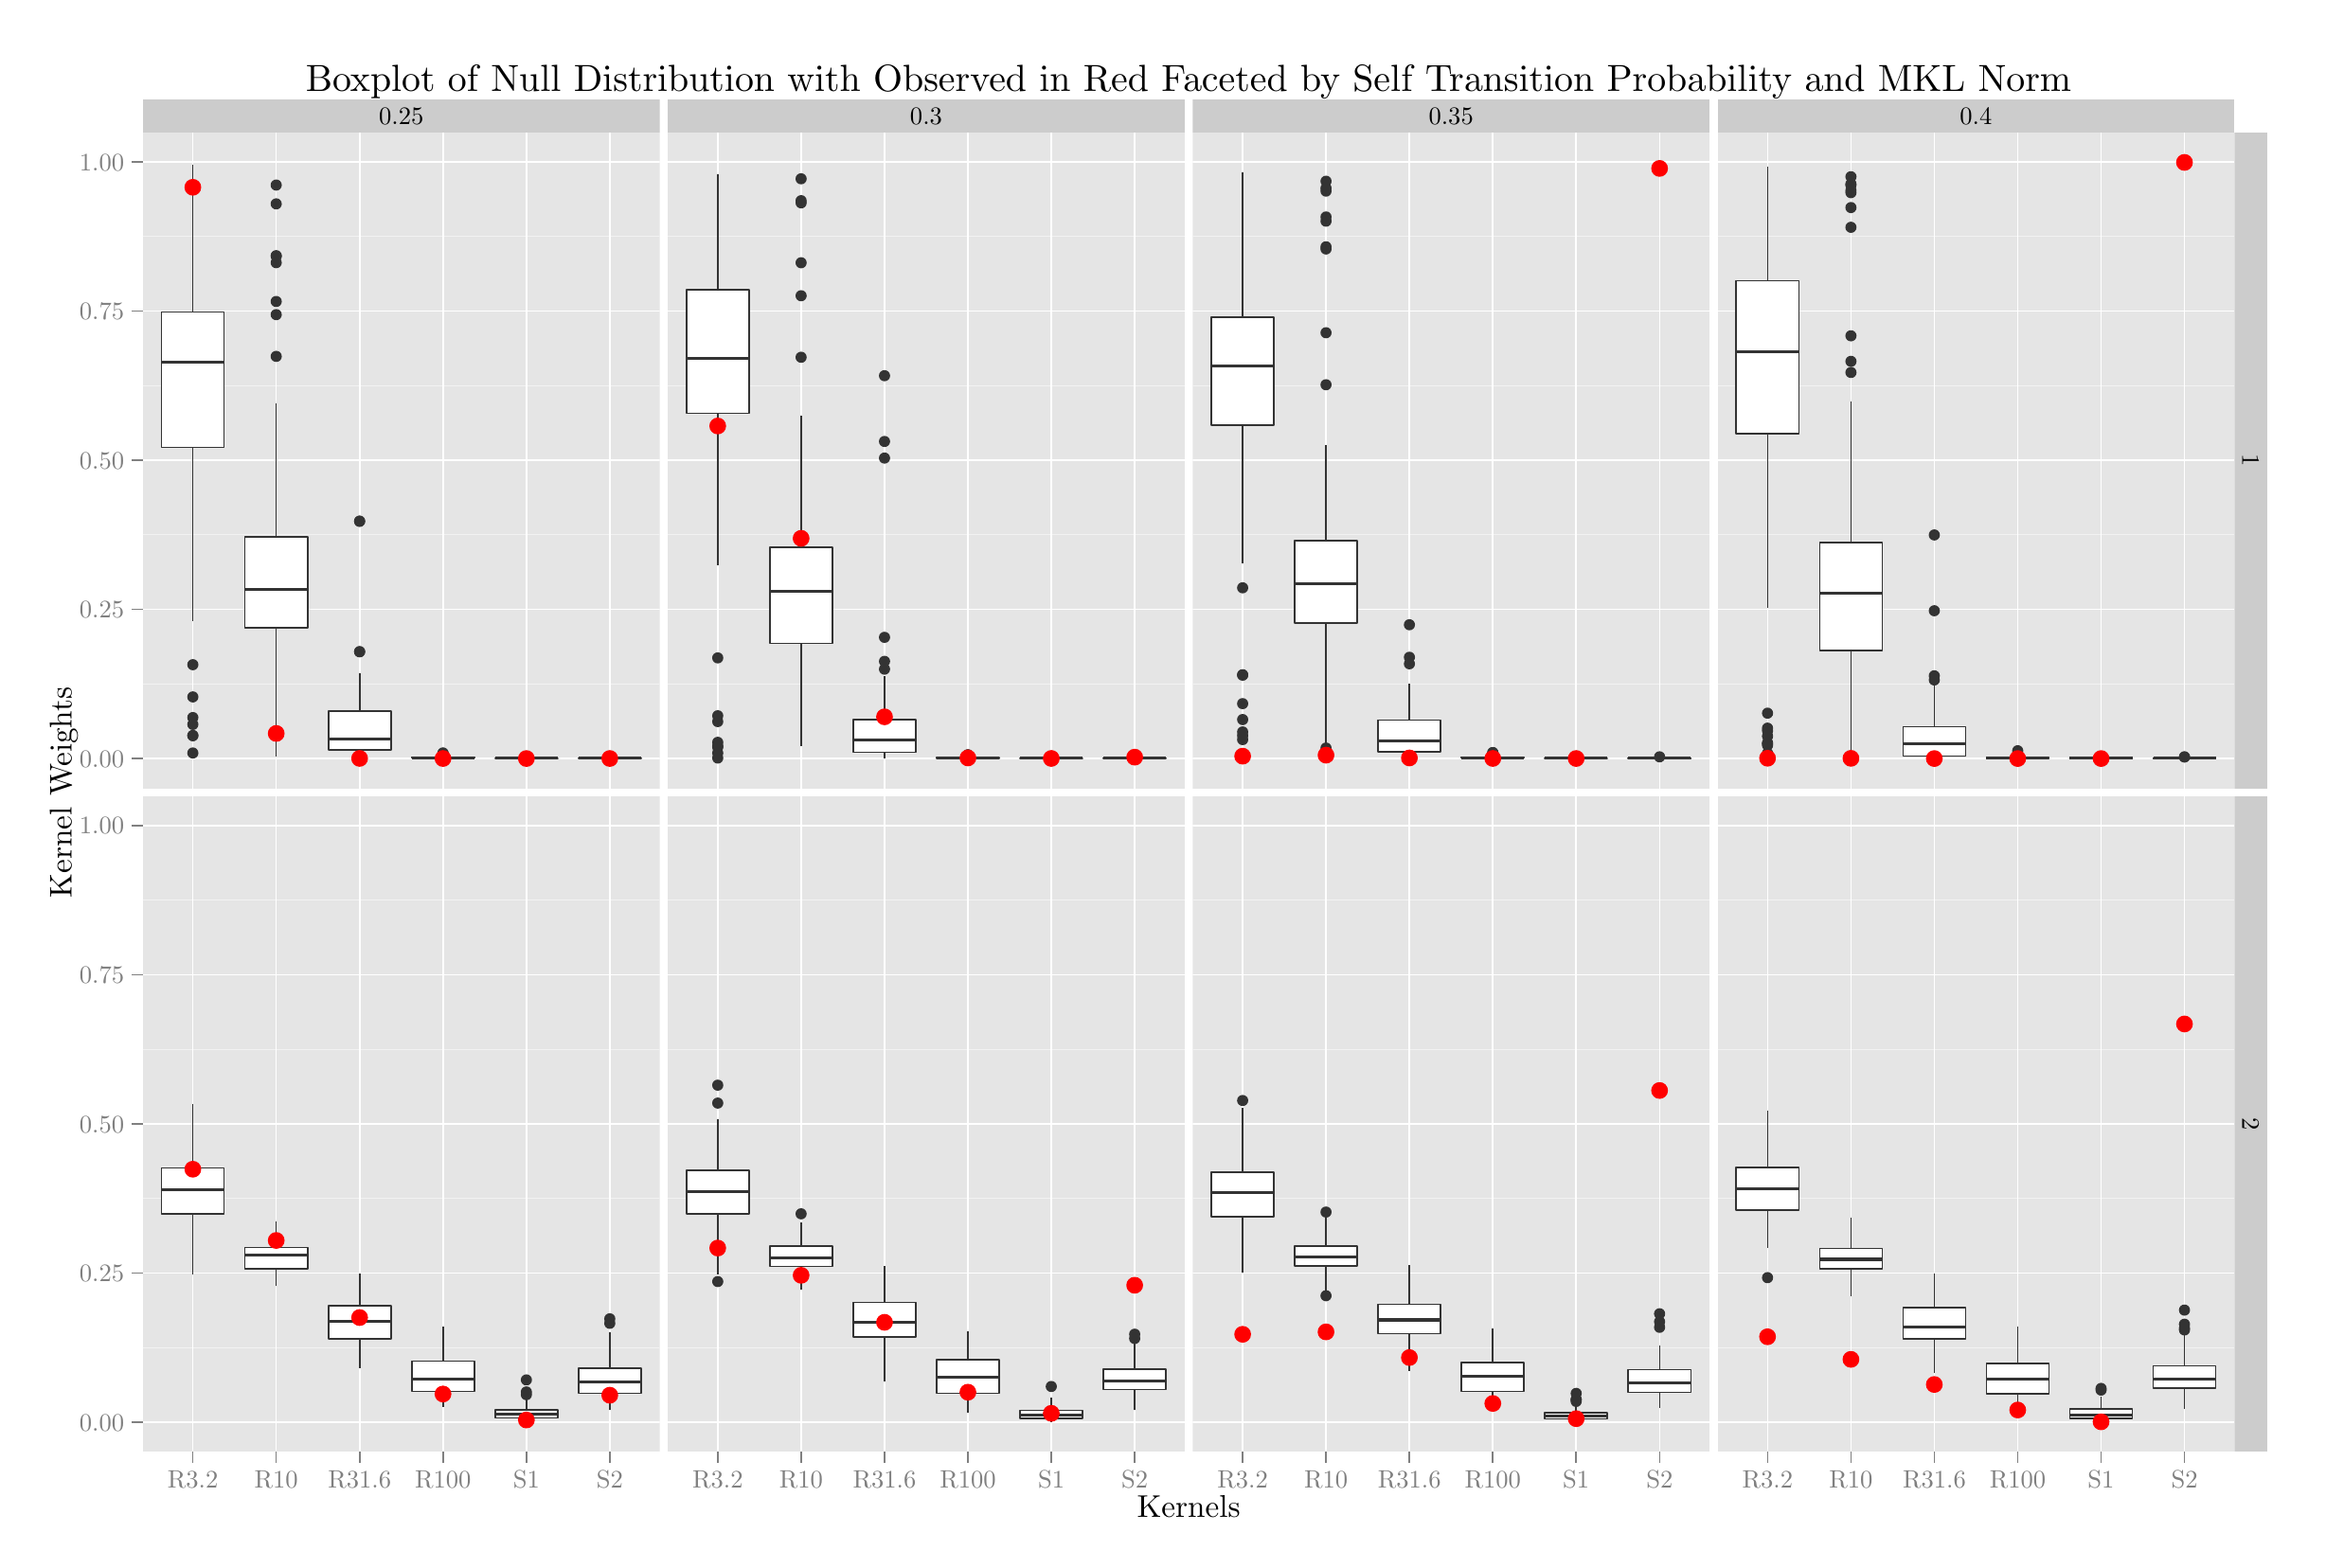
\begin{tikzpicture}[x=1pt,y=1pt]
\definecolor[named]{fillColor}{rgb}{1.00,1.00,1.00}
\path[use as bounding box,fill=fillColor,fill opacity=0.00] (0,0) rectangle (867.24,578.16);
\begin{scope}
\path[clip] (  0.00,  0.00) rectangle (867.24,578.16);
\definecolor[named]{drawColor}{rgb}{1.00,1.00,1.00}
\definecolor[named]{fillColor}{rgb}{1.00,1.00,1.00}

\path[draw=drawColor,line width= 0.6pt,line join=round,line cap=round,fill=fillColor] ( -0.00,  0.00) rectangle (867.24,578.16);
\end{scope}
\begin{scope}
\path[clip] ( 44.49,537.54) rectangle (241.75,550.17);
\definecolor[named]{fillColor}{rgb}{0.80,0.80,0.80}

\path[fill=fillColor] ( 44.49,537.54) rectangle (241.75,550.17);
\definecolor[named]{drawColor}{rgb}{0.00,0.00,0.00}

\node[text=drawColor,anchor=base,inner sep=0pt, outer sep=0pt, scale=  0.96] at (143.12,540.55) {0.25};
\end{scope}
\begin{scope}
\path[clip] (244.76,537.54) rectangle (442.02,550.17);
\definecolor[named]{fillColor}{rgb}{0.80,0.80,0.80}

\path[fill=fillColor] (244.76,537.54) rectangle (442.02,550.17);
\definecolor[named]{drawColor}{rgb}{0.00,0.00,0.00}

\node[text=drawColor,anchor=base,inner sep=0pt, outer sep=0pt, scale=  0.96] at (343.39,540.55) {0.3};
\end{scope}
\begin{scope}
\path[clip] (445.03,537.54) rectangle (642.29,550.17);
\definecolor[named]{fillColor}{rgb}{0.80,0.80,0.80}

\path[fill=fillColor] (445.03,537.54) rectangle (642.29,550.17);
\definecolor[named]{drawColor}{rgb}{0.00,0.00,0.00}

\node[text=drawColor,anchor=base,inner sep=0pt, outer sep=0pt, scale=  0.96] at (543.66,540.55) {0.35};
\end{scope}
\begin{scope}
\path[clip] (645.30,537.54) rectangle (842.56,550.17);
\definecolor[named]{fillColor}{rgb}{0.80,0.80,0.80}

\path[fill=fillColor] (645.30,537.54) rectangle (842.56,550.17);
\definecolor[named]{drawColor}{rgb}{0.00,0.00,0.00}

\node[text=drawColor,anchor=base,inner sep=0pt, outer sep=0pt, scale=  0.96] at (743.93,540.55) {0.4};
\end{scope}
\begin{scope}
\path[clip] ( 44.49,287.29) rectangle (241.75,537.54);
\definecolor[named]{fillColor}{rgb}{0.90,0.90,0.90}

\path[fill=fillColor] ( 44.49,287.29) rectangle (241.75,537.54);
\definecolor[named]{drawColor}{rgb}{0.95,0.95,0.95}

\path[draw=drawColor,line width= 0.3pt,line join=round] ( 44.49,327.13) --
	(241.75,327.13);

\path[draw=drawColor,line width= 0.3pt,line join=round] ( 44.49,384.06) --
	(241.75,384.06);

\path[draw=drawColor,line width= 0.3pt,line join=round] ( 44.49,440.99) --
	(241.75,440.99);

\path[draw=drawColor,line width= 0.3pt,line join=round] ( 44.49,497.92) --
	(241.75,497.92);
\definecolor[named]{drawColor}{rgb}{1.00,1.00,1.00}

\path[draw=drawColor,line width= 0.6pt,line join=round] ( 44.49,298.67) --
	(241.75,298.67);

\path[draw=drawColor,line width= 0.6pt,line join=round] ( 44.49,355.60) --
	(241.75,355.60);

\path[draw=drawColor,line width= 0.6pt,line join=round] ( 44.49,412.52) --
	(241.75,412.52);

\path[draw=drawColor,line width= 0.6pt,line join=round] ( 44.49,469.45) --
	(241.75,469.45);

\path[draw=drawColor,line width= 0.6pt,line join=round] ( 44.49,526.38) --
	(241.75,526.38);

\path[draw=drawColor,line width= 0.6pt,line join=round] ( 63.58,287.29) --
	( 63.58,537.54);

\path[draw=drawColor,line width= 0.6pt,line join=round] ( 95.39,287.29) --
	( 95.39,537.54);

\path[draw=drawColor,line width= 0.6pt,line join=round] (127.21,287.29) --
	(127.21,537.54);

\path[draw=drawColor,line width= 0.6pt,line join=round] (159.02,287.29) --
	(159.02,537.54);

\path[draw=drawColor,line width= 0.6pt,line join=round] (190.84,287.29) --
	(190.84,537.54);

\path[draw=drawColor,line width= 0.6pt,line join=round] (222.66,287.29) --
	(222.66,537.54);
\definecolor[named]{fillColor}{rgb}{0.20,0.20,0.20}

\path[fill=fillColor] ( 63.58,307.38) circle (  2.13);

\path[fill=fillColor] ( 63.58,314.31) circle (  2.13);

\path[fill=fillColor] ( 63.58,307.48) circle (  2.13);

\path[fill=fillColor] ( 63.58,300.79) circle (  2.13);

\path[fill=fillColor] ( 63.58,334.49) circle (  2.13);

\path[fill=fillColor] ( 63.58,311.70) circle (  2.13);

\path[fill=fillColor] ( 63.58,322.19) circle (  2.13);
\definecolor[named]{drawColor}{rgb}{0.20,0.20,0.20}

\path[draw=drawColor,line width= 0.6pt,line join=round,fill=fillColor] ( 63.58,469.10) -- ( 63.58,525.42);

\path[draw=drawColor,line width= 0.6pt,line join=round,fill=fillColor] ( 63.58,417.47) -- ( 63.58,351.27);
\definecolor[named]{fillColor}{rgb}{1.00,1.00,1.00}

\path[draw=drawColor,line width= 0.6pt,line join=round,line cap=round,fill=fillColor] ( 51.64,469.10) --
	( 51.64,417.47) --
	( 75.51,417.47) --
	( 75.51,469.10) --
	( 51.64,469.10) --
	cycle;
\definecolor[named]{fillColor}{rgb}{0.20,0.20,0.20}

\path[draw=drawColor,line width= 1.1pt,line join=round,fill=fillColor] ( 51.64,449.89) -- ( 75.51,449.89);

\path[fill=fillColor] ( 95.39,517.53) circle (  2.13);

\path[fill=fillColor] ( 95.39,510.35) circle (  2.13);

\path[fill=fillColor] ( 95.39,490.57) circle (  2.13);

\path[fill=fillColor] ( 95.39,473.10) circle (  2.13);

\path[fill=fillColor] ( 95.39,468.08) circle (  2.13);

\path[fill=fillColor] ( 95.39,490.38) circle (  2.13);

\path[fill=fillColor] ( 95.39,452.15) circle (  2.13);

\path[fill=fillColor] ( 95.39,487.91) circle (  2.13);

\path[draw=drawColor,line width= 0.6pt,line join=round,fill=fillColor] ( 95.39,383.34) -- ( 95.39,434.24);

\path[draw=drawColor,line width= 0.6pt,line join=round,fill=fillColor] ( 95.39,348.56) -- ( 95.39,299.60);
\definecolor[named]{fillColor}{rgb}{1.00,1.00,1.00}

\path[draw=drawColor,line width= 0.6pt,line join=round,line cap=round,fill=fillColor] ( 83.46,383.34) --
	( 83.46,348.56) --
	(107.32,348.56) --
	(107.32,383.34) --
	( 83.46,383.34) --
	cycle;
\definecolor[named]{fillColor}{rgb}{0.20,0.20,0.20}

\path[draw=drawColor,line width= 1.1pt,line join=round,fill=fillColor] ( 83.46,363.31) -- (107.32,363.31);

\path[fill=fillColor] (127.21,389.19) circle (  2.13);

\path[fill=fillColor] (127.21,339.46) circle (  2.13);

\path[fill=fillColor] (127.21,389.29) circle (  2.13);

\path[fill=fillColor] (127.21,339.43) circle (  2.13);

\path[draw=drawColor,line width= 0.6pt,line join=round,fill=fillColor] (127.21,316.88) -- (127.21,331.41);

\path[draw=drawColor,line width= 0.6pt,line join=round,fill=fillColor] (127.21,301.99) -- (127.21,298.68);
\definecolor[named]{fillColor}{rgb}{1.00,1.00,1.00}

\path[draw=drawColor,line width= 0.6pt,line join=round,line cap=round,fill=fillColor] (115.28,316.88) --
	(115.28,301.99) --
	(139.14,301.99) --
	(139.14,316.88) --
	(115.28,316.88) --
	cycle;
\definecolor[named]{fillColor}{rgb}{0.20,0.20,0.20}

\path[draw=drawColor,line width= 1.1pt,line join=round,fill=fillColor] (115.28,306.04) -- (139.14,306.04);

\path[fill=fillColor] (159.02,300.36) circle (  2.13);

\path[fill=fillColor] (159.02,300.29) circle (  2.13);

\path[fill=fillColor] (159.02,299.94) circle (  2.13);

\path[fill=fillColor] (159.02,300.17) circle (  2.13);

\path[fill=fillColor] (159.02,300.68) circle (  2.13);

\path[fill=fillColor] (159.02,300.80) circle (  2.13);

\path[fill=fillColor] (159.02,300.49) circle (  2.13);

\path[fill=fillColor] (159.02,299.97) circle (  2.13);

\path[fill=fillColor] (159.02,300.05) circle (  2.13);

\path[draw=drawColor,line width= 0.6pt,line join=round,fill=fillColor] (159.02,299.29) -- (159.02,299.82);

\path[draw=drawColor,line width= 0.6pt,line join=round,fill=fillColor] (159.02,298.86) -- (159.02,298.67);
\definecolor[named]{fillColor}{rgb}{1.00,1.00,1.00}

\path[draw=drawColor,line width= 0.6pt,line join=round,line cap=round,fill=fillColor] (147.09,299.29) --
	(147.09,298.86) --
	(170.95,298.86) --
	(170.95,299.29) --
	(147.09,299.29) --
	cycle;
\definecolor[named]{fillColor}{rgb}{0.20,0.20,0.20}

\path[draw=drawColor,line width= 1.1pt,line join=round,fill=fillColor] (147.09,298.99) -- (170.95,298.99);

\path[draw=drawColor,line width= 0.6pt,line join=round,fill=fillColor] (190.84,298.83) -- (190.84,298.97);

\path[draw=drawColor,line width= 0.6pt,line join=round,fill=fillColor] (190.84,298.71) -- (190.84,298.67);
\definecolor[named]{fillColor}{rgb}{1.00,1.00,1.00}

\path[draw=drawColor,line width= 0.6pt,line join=round,line cap=round,fill=fillColor] (178.91,298.83) --
	(178.91,298.71) --
	(202.77,298.71) --
	(202.77,298.83) --
	(178.91,298.83) --
	cycle;
\definecolor[named]{fillColor}{rgb}{0.20,0.20,0.20}

\path[draw=drawColor,line width= 1.1pt,line join=round,fill=fillColor] (178.91,298.78) -- (202.77,298.78);

\path[fill=fillColor] (222.66,299.26) circle (  2.13);

\path[draw=drawColor,line width= 0.6pt,line join=round,fill=fillColor] (222.66,298.94) -- (222.66,299.16);

\path[draw=drawColor,line width= 0.6pt,line join=round,fill=fillColor] (222.66,298.73) -- (222.66,298.67);
\definecolor[named]{fillColor}{rgb}{1.00,1.00,1.00}

\path[draw=drawColor,line width= 0.6pt,line join=round,line cap=round,fill=fillColor] (210.73,298.94) --
	(210.73,298.73) --
	(234.59,298.73) --
	(234.59,298.94) --
	(210.73,298.94) --
	cycle;
\definecolor[named]{fillColor}{rgb}{0.20,0.20,0.20}

\path[draw=drawColor,line width= 1.1pt,line join=round,fill=fillColor] (210.73,298.86) -- (234.59,298.86);
\definecolor[named]{fillColor}{rgb}{1.00,0.00,0.00}

\path[fill=fillColor] ( 63.58,516.68) circle (  3.20);

\path[fill=fillColor] ( 95.39,308.25) circle (  3.20);

\path[fill=fillColor] (127.21,298.73) circle (  3.20);

\path[fill=fillColor] (159.02,298.69) circle (  3.20);

\path[fill=fillColor] (190.84,298.68) circle (  3.20);

\path[fill=fillColor] (222.66,298.69) circle (  3.20);
\end{scope}
\begin{scope}
\path[clip] ( 44.49, 34.03) rectangle (241.75,284.28);
\definecolor[named]{fillColor}{rgb}{0.90,0.90,0.90}

\path[fill=fillColor] ( 44.49, 34.03) rectangle (241.75,284.28);
\definecolor[named]{drawColor}{rgb}{0.95,0.95,0.95}

\path[draw=drawColor,line width= 0.3pt,line join=round] ( 44.49, 73.87) --
	(241.75, 73.87);

\path[draw=drawColor,line width= 0.3pt,line join=round] ( 44.49,130.80) --
	(241.75,130.80);

\path[draw=drawColor,line width= 0.3pt,line join=round] ( 44.49,187.73) --
	(241.75,187.73);

\path[draw=drawColor,line width= 0.3pt,line join=round] ( 44.49,244.66) --
	(241.75,244.66);
\definecolor[named]{drawColor}{rgb}{1.00,1.00,1.00}

\path[draw=drawColor,line width= 0.6pt,line join=round] ( 44.49, 45.41) --
	(241.75, 45.41);

\path[draw=drawColor,line width= 0.6pt,line join=round] ( 44.49,102.34) --
	(241.75,102.34);

\path[draw=drawColor,line width= 0.6pt,line join=round] ( 44.49,159.26) --
	(241.75,159.26);

\path[draw=drawColor,line width= 0.6pt,line join=round] ( 44.49,216.19) --
	(241.75,216.19);

\path[draw=drawColor,line width= 0.6pt,line join=round] ( 44.49,273.12) --
	(241.75,273.12);

\path[draw=drawColor,line width= 0.6pt,line join=round] ( 63.58, 34.03) --
	( 63.58,284.28);

\path[draw=drawColor,line width= 0.6pt,line join=round] ( 95.39, 34.03) --
	( 95.39,284.28);

\path[draw=drawColor,line width= 0.6pt,line join=round] (127.21, 34.03) --
	(127.21,284.28);

\path[draw=drawColor,line width= 0.6pt,line join=round] (159.02, 34.03) --
	(159.02,284.28);

\path[draw=drawColor,line width= 0.6pt,line join=round] (190.84, 34.03) --
	(190.84,284.28);

\path[draw=drawColor,line width= 0.6pt,line join=round] (222.66, 34.03) --
	(222.66,284.28);
\definecolor[named]{drawColor}{rgb}{0.20,0.20,0.20}
\definecolor[named]{fillColor}{rgb}{0.20,0.20,0.20}

\path[draw=drawColor,line width= 0.6pt,line join=round,fill=fillColor] ( 63.58,142.43) -- ( 63.58,166.88);

\path[draw=drawColor,line width= 0.6pt,line join=round,fill=fillColor] ( 63.58,124.91) -- ( 63.58,101.89);
\definecolor[named]{fillColor}{rgb}{1.00,1.00,1.00}

\path[draw=drawColor,line width= 0.6pt,line join=round,line cap=round,fill=fillColor] ( 51.64,142.43) --
	( 51.64,124.91) --
	( 75.51,124.91) --
	( 75.51,142.43) --
	( 51.64,142.43) --
	cycle;
\definecolor[named]{fillColor}{rgb}{0.20,0.20,0.20}

\path[draw=drawColor,line width= 1.1pt,line join=round,fill=fillColor] ( 51.64,134.06) -- ( 75.51,134.06);

\path[draw=drawColor,line width= 0.6pt,line join=round,fill=fillColor] ( 95.39,112.12) -- ( 95.39,122.17);

\path[draw=drawColor,line width= 0.6pt,line join=round,fill=fillColor] ( 95.39,104.05) -- ( 95.39, 97.30);
\definecolor[named]{fillColor}{rgb}{1.00,1.00,1.00}

\path[draw=drawColor,line width= 0.6pt,line join=round,line cap=round,fill=fillColor] ( 83.46,112.12) --
	( 83.46,104.05) --
	(107.32,104.05) --
	(107.32,112.12) --
	( 83.46,112.12) --
	cycle;
\definecolor[named]{fillColor}{rgb}{0.20,0.20,0.20}

\path[draw=drawColor,line width= 1.1pt,line join=round,fill=fillColor] ( 83.46,109.03) -- (107.32,109.03);

\path[draw=drawColor,line width= 0.6pt,line join=round,fill=fillColor] (127.21, 89.76) -- (127.21,101.99);

\path[draw=drawColor,line width= 0.6pt,line join=round,fill=fillColor] (127.21, 77.13) -- (127.21, 66.07);
\definecolor[named]{fillColor}{rgb}{1.00,1.00,1.00}

\path[draw=drawColor,line width= 0.6pt,line join=round,line cap=round,fill=fillColor] (115.28, 89.76) --
	(115.28, 77.13) --
	(139.14, 77.13) --
	(139.14, 89.76) --
	(115.28, 89.76) --
	cycle;
\definecolor[named]{fillColor}{rgb}{0.20,0.20,0.20}

\path[draw=drawColor,line width= 1.1pt,line join=round,fill=fillColor] (115.28, 83.75) -- (139.14, 83.75);

\path[draw=drawColor,line width= 0.6pt,line join=round,fill=fillColor] (159.02, 68.66) -- (159.02, 81.78);

\path[draw=drawColor,line width= 0.6pt,line join=round,fill=fillColor] (159.02, 57.13) -- (159.02, 51.25);
\definecolor[named]{fillColor}{rgb}{1.00,1.00,1.00}

\path[draw=drawColor,line width= 0.6pt,line join=round,line cap=round,fill=fillColor] (147.09, 68.66) --
	(147.09, 57.13) --
	(170.95, 57.13) --
	(170.95, 68.66) --
	(147.09, 68.66) --
	cycle;
\definecolor[named]{fillColor}{rgb}{0.20,0.20,0.20}

\path[draw=drawColor,line width= 1.1pt,line join=round,fill=fillColor] (147.09, 61.99) -- (170.95, 61.99);

\path[fill=fillColor] (190.84, 55.91) circle (  2.13);

\path[fill=fillColor] (190.84, 61.55) circle (  2.13);

\path[fill=fillColor] (190.84, 56.96) circle (  2.13);

\path[draw=drawColor,line width= 0.6pt,line join=round,fill=fillColor] (190.84, 50.14) -- (190.84, 54.71);

\path[draw=drawColor,line width= 0.6pt,line join=round,fill=fillColor] (190.84, 47.08) -- (190.84, 45.57);
\definecolor[named]{fillColor}{rgb}{1.00,1.00,1.00}

\path[draw=drawColor,line width= 0.6pt,line join=round,line cap=round,fill=fillColor] (178.91, 50.14) --
	(178.91, 47.08) --
	(202.77, 47.08) --
	(202.77, 50.14) --
	(178.91, 50.14) --
	cycle;
\definecolor[named]{fillColor}{rgb}{0.20,0.20,0.20}

\path[draw=drawColor,line width= 1.1pt,line join=round,fill=fillColor] (178.91, 48.41) -- (202.77, 48.41);

\path[fill=fillColor] (222.66, 84.85) circle (  2.13);

\path[fill=fillColor] (222.66, 83.13) circle (  2.13);

\path[draw=drawColor,line width= 0.6pt,line join=round,fill=fillColor] (222.66, 65.95) -- (222.66, 79.86);

\path[draw=drawColor,line width= 0.6pt,line join=round,fill=fillColor] (222.66, 56.46) -- (222.66, 49.93);
\definecolor[named]{fillColor}{rgb}{1.00,1.00,1.00}

\path[draw=drawColor,line width= 0.6pt,line join=round,line cap=round,fill=fillColor] (210.73, 65.95) --
	(210.73, 56.46) --
	(234.59, 56.46) --
	(234.59, 65.95) --
	(210.73, 65.95) --
	cycle;
\definecolor[named]{fillColor}{rgb}{0.20,0.20,0.20}

\path[draw=drawColor,line width= 1.1pt,line join=round,fill=fillColor] (210.73, 60.61) -- (234.59, 60.61);
\definecolor[named]{fillColor}{rgb}{1.00,0.00,0.00}

\path[fill=fillColor] ( 63.58,141.95) circle (  3.20);

\path[fill=fillColor] ( 95.39,114.76) circle (  3.20);

\path[fill=fillColor] (127.21, 85.34) circle (  3.20);

\path[fill=fillColor] (159.02, 56.16) circle (  3.20);

\path[fill=fillColor] (190.84, 46.25) circle (  3.20);

\path[fill=fillColor] (222.66, 55.70) circle (  3.20);
\end{scope}
\begin{scope}
\path[clip] (244.76,287.29) rectangle (442.02,537.54);
\definecolor[named]{fillColor}{rgb}{0.90,0.90,0.90}

\path[fill=fillColor] (244.76,287.29) rectangle (442.02,537.54);
\definecolor[named]{drawColor}{rgb}{0.95,0.95,0.95}

\path[draw=drawColor,line width= 0.3pt,line join=round] (244.76,327.13) --
	(442.02,327.13);

\path[draw=drawColor,line width= 0.3pt,line join=round] (244.76,384.06) --
	(442.02,384.06);

\path[draw=drawColor,line width= 0.3pt,line join=round] (244.76,440.99) --
	(442.02,440.99);

\path[draw=drawColor,line width= 0.3pt,line join=round] (244.76,497.92) --
	(442.02,497.92);
\definecolor[named]{drawColor}{rgb}{1.00,1.00,1.00}

\path[draw=drawColor,line width= 0.6pt,line join=round] (244.76,298.67) --
	(442.02,298.67);

\path[draw=drawColor,line width= 0.6pt,line join=round] (244.76,355.60) --
	(442.02,355.60);

\path[draw=drawColor,line width= 0.6pt,line join=round] (244.76,412.52) --
	(442.02,412.52);

\path[draw=drawColor,line width= 0.6pt,line join=round] (244.76,469.45) --
	(442.02,469.45);

\path[draw=drawColor,line width= 0.6pt,line join=round] (244.76,526.38) --
	(442.02,526.38);

\path[draw=drawColor,line width= 0.6pt,line join=round] (263.85,287.29) --
	(263.85,537.54);

\path[draw=drawColor,line width= 0.6pt,line join=round] (295.66,287.29) --
	(295.66,537.54);

\path[draw=drawColor,line width= 0.6pt,line join=round] (327.48,287.29) --
	(327.48,537.54);

\path[draw=drawColor,line width= 0.6pt,line join=round] (359.30,287.29) --
	(359.30,537.54);

\path[draw=drawColor,line width= 0.6pt,line join=round] (391.11,287.29) --
	(391.11,537.54);

\path[draw=drawColor,line width= 0.6pt,line join=round] (422.93,287.29) --
	(422.93,537.54);
\definecolor[named]{fillColor}{rgb}{0.20,0.20,0.20}

\path[fill=fillColor] (263.85,312.78) circle (  2.13);

\path[fill=fillColor] (263.85,303.05) circle (  2.13);

\path[fill=fillColor] (263.85,298.86) circle (  2.13);

\path[fill=fillColor] (263.85,315.00) circle (  2.13);

\path[fill=fillColor] (263.85,300.79) circle (  2.13);

\path[fill=fillColor] (263.85,304.86) circle (  2.13);

\path[fill=fillColor] (263.85,337.08) circle (  2.13);

\path[fill=fillColor] (263.85,303.44) circle (  2.13);
\definecolor[named]{drawColor}{rgb}{0.20,0.20,0.20}

\path[draw=drawColor,line width= 0.6pt,line join=round,fill=fillColor] (263.85,477.54) -- (263.85,521.61);

\path[draw=drawColor,line width= 0.6pt,line join=round,fill=fillColor] (263.85,430.46) -- (263.85,372.39);
\definecolor[named]{fillColor}{rgb}{1.00,1.00,1.00}

\path[draw=drawColor,line width= 0.6pt,line join=round,line cap=round,fill=fillColor] (251.92,477.54) --
	(251.92,430.46) --
	(275.78,430.46) --
	(275.78,477.54) --
	(251.92,477.54) --
	cycle;
\definecolor[named]{fillColor}{rgb}{0.20,0.20,0.20}

\path[draw=drawColor,line width= 1.1pt,line join=round,fill=fillColor] (251.92,451.30) -- (275.78,451.30);

\path[fill=fillColor] (295.66,511.56) circle (  2.13);

\path[fill=fillColor] (295.66,451.82) circle (  2.13);

\path[fill=fillColor] (295.66,510.74) circle (  2.13);

\path[fill=fillColor] (295.66,519.92) circle (  2.13);

\path[fill=fillColor] (295.66,487.88) circle (  2.13);

\path[fill=fillColor] (295.66,475.29) circle (  2.13);

\path[draw=drawColor,line width= 0.6pt,line join=round,fill=fillColor] (295.66,379.19) -- (295.66,429.63);

\path[draw=drawColor,line width= 0.6pt,line join=round,fill=fillColor] (295.66,342.57) -- (295.66,303.36);
\definecolor[named]{fillColor}{rgb}{1.00,1.00,1.00}

\path[draw=drawColor,line width= 0.6pt,line join=round,line cap=round,fill=fillColor] (283.73,379.19) --
	(283.73,342.57) --
	(307.59,342.57) --
	(307.59,379.19) --
	(283.73,379.19) --
	cycle;
\definecolor[named]{fillColor}{rgb}{0.20,0.20,0.20}

\path[draw=drawColor,line width= 1.1pt,line join=round,fill=fillColor] (283.73,362.49) -- (307.59,362.49);

\path[fill=fillColor] (327.48,335.76) circle (  2.13);

\path[fill=fillColor] (327.48,444.77) circle (  2.13);

\path[fill=fillColor] (327.48,332.78) circle (  2.13);

\path[fill=fillColor] (327.48,419.68) circle (  2.13);

\path[fill=fillColor] (327.48,413.34) circle (  2.13);

\path[fill=fillColor] (327.48,344.93) circle (  2.13);

\path[draw=drawColor,line width= 0.6pt,line join=round,fill=fillColor] (327.48,313.54) -- (327.48,330.05);

\path[draw=drawColor,line width= 0.6pt,line join=round,fill=fillColor] (327.48,301.08) -- (327.48,298.70);
\definecolor[named]{fillColor}{rgb}{1.00,1.00,1.00}

\path[draw=drawColor,line width= 0.6pt,line join=round,line cap=round,fill=fillColor] (315.55,313.54) --
	(315.55,301.08) --
	(339.41,301.08) --
	(339.41,313.54) --
	(315.55,313.54) --
	cycle;
\definecolor[named]{fillColor}{rgb}{0.20,0.20,0.20}

\path[draw=drawColor,line width= 1.1pt,line join=round,fill=fillColor] (315.55,305.87) -- (339.41,305.87);

\path[fill=fillColor] (359.30,300.05) circle (  2.13);

\path[fill=fillColor] (359.30,300.11) circle (  2.13);

\path[fill=fillColor] (359.30,299.86) circle (  2.13);

\path[fill=fillColor] (359.30,299.72) circle (  2.13);

\path[fill=fillColor] (359.30,299.80) circle (  2.13);

\path[fill=fillColor] (359.30,299.71) circle (  2.13);

\path[draw=drawColor,line width= 0.6pt,line join=round,fill=fillColor] (359.30,299.16) -- (359.30,299.67);

\path[draw=drawColor,line width= 0.6pt,line join=round,fill=fillColor] (359.30,298.81) -- (359.30,298.68);
\definecolor[named]{fillColor}{rgb}{1.00,1.00,1.00}

\path[draw=drawColor,line width= 0.6pt,line join=round,line cap=round,fill=fillColor] (347.36,299.16) --
	(347.36,298.81) --
	(371.23,298.81) --
	(371.23,299.16) --
	(347.36,299.16) --
	cycle;
\definecolor[named]{fillColor}{rgb}{0.20,0.20,0.20}

\path[draw=drawColor,line width= 1.1pt,line join=round,fill=fillColor] (347.36,298.96) -- (371.23,298.96);

\path[fill=fillColor] (391.11,299.17) circle (  2.13);

\path[fill=fillColor] (391.11,299.08) circle (  2.13);

\path[draw=drawColor,line width= 0.6pt,line join=round,fill=fillColor] (391.11,298.82) -- (391.11,298.97);

\path[draw=drawColor,line width= 0.6pt,line join=round,fill=fillColor] (391.11,298.71) -- (391.11,298.67);
\definecolor[named]{fillColor}{rgb}{1.00,1.00,1.00}

\path[draw=drawColor,line width= 0.6pt,line join=round,line cap=round,fill=fillColor] (379.18,298.82) --
	(379.18,298.71) --
	(403.04,298.71) --
	(403.04,298.82) --
	(379.18,298.82) --
	cycle;
\definecolor[named]{fillColor}{rgb}{0.20,0.20,0.20}

\path[draw=drawColor,line width= 1.1pt,line join=round,fill=fillColor] (379.18,298.77) -- (403.04,298.77);

\path[fill=fillColor] (422.93,299.90) circle (  2.13);

\path[fill=fillColor] (422.93,299.36) circle (  2.13);

\path[fill=fillColor] (422.93,299.32) circle (  2.13);

\path[fill=fillColor] (422.93,299.61) circle (  2.13);

\path[draw=drawColor,line width= 0.6pt,line join=round,fill=fillColor] (422.93,298.90) -- (422.93,299.07);

\path[draw=drawColor,line width= 0.6pt,line join=round,fill=fillColor] (422.93,298.74) -- (422.93,298.67);
\definecolor[named]{fillColor}{rgb}{1.00,1.00,1.00}

\path[draw=drawColor,line width= 0.6pt,line join=round,line cap=round,fill=fillColor] (411.00,298.90) --
	(411.00,298.74) --
	(434.86,298.74) --
	(434.86,298.90) --
	(411.00,298.90) --
	cycle;
\definecolor[named]{fillColor}{rgb}{0.20,0.20,0.20}

\path[draw=drawColor,line width= 1.1pt,line join=round,fill=fillColor] (411.00,298.84) -- (434.86,298.84);
\definecolor[named]{fillColor}{rgb}{1.00,0.00,0.00}

\path[fill=fillColor] (263.85,425.59) circle (  3.20);

\path[fill=fillColor] (295.66,382.71) circle (  3.20);

\path[fill=fillColor] (327.48,314.59) circle (  3.20);

\path[fill=fillColor] (359.30,298.91) circle (  3.20);

\path[fill=fillColor] (391.11,298.71) circle (  3.20);

\path[fill=fillColor] (422.93,299.20) circle (  3.20);
\end{scope}
\begin{scope}
\path[clip] (244.76, 34.03) rectangle (442.02,284.28);
\definecolor[named]{fillColor}{rgb}{0.90,0.90,0.90}

\path[fill=fillColor] (244.76, 34.03) rectangle (442.02,284.28);
\definecolor[named]{drawColor}{rgb}{0.95,0.95,0.95}

\path[draw=drawColor,line width= 0.3pt,line join=round] (244.76, 73.87) --
	(442.02, 73.87);

\path[draw=drawColor,line width= 0.3pt,line join=round] (244.76,130.80) --
	(442.02,130.80);

\path[draw=drawColor,line width= 0.3pt,line join=round] (244.76,187.73) --
	(442.02,187.73);

\path[draw=drawColor,line width= 0.3pt,line join=round] (244.76,244.66) --
	(442.02,244.66);
\definecolor[named]{drawColor}{rgb}{1.00,1.00,1.00}

\path[draw=drawColor,line width= 0.6pt,line join=round] (244.76, 45.41) --
	(442.02, 45.41);

\path[draw=drawColor,line width= 0.6pt,line join=round] (244.76,102.34) --
	(442.02,102.34);

\path[draw=drawColor,line width= 0.6pt,line join=round] (244.76,159.26) --
	(442.02,159.26);

\path[draw=drawColor,line width= 0.6pt,line join=round] (244.76,216.19) --
	(442.02,216.19);

\path[draw=drawColor,line width= 0.6pt,line join=round] (244.76,273.12) --
	(442.02,273.12);

\path[draw=drawColor,line width= 0.6pt,line join=round] (263.85, 34.03) --
	(263.85,284.28);

\path[draw=drawColor,line width= 0.6pt,line join=round] (295.66, 34.03) --
	(295.66,284.28);

\path[draw=drawColor,line width= 0.6pt,line join=round] (327.48, 34.03) --
	(327.48,284.28);

\path[draw=drawColor,line width= 0.6pt,line join=round] (359.30, 34.03) --
	(359.30,284.28);

\path[draw=drawColor,line width= 0.6pt,line join=round] (391.11, 34.03) --
	(391.11,284.28);

\path[draw=drawColor,line width= 0.6pt,line join=round] (422.93, 34.03) --
	(422.93,284.28);
\definecolor[named]{fillColor}{rgb}{0.20,0.20,0.20}

\path[fill=fillColor] (263.85,174.02) circle (  2.13);

\path[fill=fillColor] (263.85,167.19) circle (  2.13);

\path[fill=fillColor] (263.85, 99.08) circle (  2.13);
\definecolor[named]{drawColor}{rgb}{0.20,0.20,0.20}

\path[draw=drawColor,line width= 0.6pt,line join=round,fill=fillColor] (263.85,141.42) -- (263.85,161.04);

\path[draw=drawColor,line width= 0.6pt,line join=round,fill=fillColor] (263.85,125.00) -- (263.85,101.89);
\definecolor[named]{fillColor}{rgb}{1.00,1.00,1.00}

\path[draw=drawColor,line width= 0.6pt,line join=round,line cap=round,fill=fillColor] (251.92,141.42) --
	(251.92,125.00) --
	(275.78,125.00) --
	(275.78,141.42) --
	(251.92,141.42) --
	cycle;
\definecolor[named]{fillColor}{rgb}{0.20,0.20,0.20}

\path[draw=drawColor,line width= 1.1pt,line join=round,fill=fillColor] (251.92,133.50) -- (275.78,133.50);

\path[fill=fillColor] (295.66,124.93) circle (  2.13);

\path[draw=drawColor,line width= 0.6pt,line join=round,fill=fillColor] (295.66,112.62) -- (295.66,121.75);

\path[draw=drawColor,line width= 0.6pt,line join=round,fill=fillColor] (295.66,104.82) -- (295.66, 95.83);
\definecolor[named]{fillColor}{rgb}{1.00,1.00,1.00}

\path[draw=drawColor,line width= 0.6pt,line join=round,line cap=round,fill=fillColor] (283.73,112.62) --
	(283.73,104.82) --
	(307.59,104.82) --
	(307.59,112.62) --
	(283.73,112.62) --
	cycle;
\definecolor[named]{fillColor}{rgb}{0.20,0.20,0.20}

\path[draw=drawColor,line width= 1.1pt,line join=round,fill=fillColor] (283.73,108.02) -- (307.59,108.02);

\path[draw=drawColor,line width= 0.6pt,line join=round,fill=fillColor] (327.48, 91.06) -- (327.48,104.98);

\path[draw=drawColor,line width= 0.6pt,line join=round,fill=fillColor] (327.48, 77.82) -- (327.48, 61.03);
\definecolor[named]{fillColor}{rgb}{1.00,1.00,1.00}

\path[draw=drawColor,line width= 0.6pt,line join=round,line cap=round,fill=fillColor] (315.55, 91.06) --
	(315.55, 77.82) --
	(339.41, 77.82) --
	(339.41, 91.06) --
	(315.55, 91.06) --
	cycle;
\definecolor[named]{fillColor}{rgb}{0.20,0.20,0.20}

\path[draw=drawColor,line width= 1.1pt,line join=round,fill=fillColor] (315.55, 83.58) -- (339.41, 83.58);

\path[draw=drawColor,line width= 0.6pt,line join=round,fill=fillColor] (359.30, 69.18) -- (359.30, 80.17);

\path[draw=drawColor,line width= 0.6pt,line join=round,fill=fillColor] (359.30, 56.38) -- (359.30, 48.93);
\definecolor[named]{fillColor}{rgb}{1.00,1.00,1.00}

\path[draw=drawColor,line width= 0.6pt,line join=round,line cap=round,fill=fillColor] (347.36, 69.18) --
	(347.36, 56.38) --
	(371.23, 56.38) --
	(371.23, 69.18) --
	(347.36, 69.18) --
	cycle;
\definecolor[named]{fillColor}{rgb}{0.20,0.20,0.20}

\path[draw=drawColor,line width= 1.1pt,line join=round,fill=fillColor] (347.36, 62.45) -- (371.23, 62.45);

\path[fill=fillColor] (391.11, 59.03) circle (  2.13);

\path[draw=drawColor,line width= 0.6pt,line join=round,fill=fillColor] (391.11, 49.97) -- (391.11, 54.75);

\path[draw=drawColor,line width= 0.6pt,line join=round,fill=fillColor] (391.11, 46.78) -- (391.11, 45.54);
\definecolor[named]{fillColor}{rgb}{1.00,1.00,1.00}

\path[draw=drawColor,line width= 0.6pt,line join=round,line cap=round,fill=fillColor] (379.18, 49.97) --
	(379.18, 46.78) --
	(403.04, 46.78) --
	(403.04, 49.97) --
	(379.18, 49.97) --
	cycle;
\definecolor[named]{fillColor}{rgb}{0.20,0.20,0.20}

\path[draw=drawColor,line width= 1.1pt,line join=round,fill=fillColor] (379.18, 48.23) -- (403.04, 48.23);

\path[fill=fillColor] (422.93, 77.34) circle (  2.13);

\path[fill=fillColor] (422.93, 78.99) circle (  2.13);

\path[draw=drawColor,line width= 0.6pt,line join=round,fill=fillColor] (422.93, 65.57) -- (422.93, 76.98);

\path[draw=drawColor,line width= 0.6pt,line join=round,fill=fillColor] (422.93, 57.90) -- (422.93, 50.19);
\definecolor[named]{fillColor}{rgb}{1.00,1.00,1.00}

\path[draw=drawColor,line width= 0.6pt,line join=round,line cap=round,fill=fillColor] (411.00, 65.57) --
	(411.00, 57.90) --
	(434.86, 57.90) --
	(434.86, 65.57) --
	(411.00, 65.57) --
	cycle;
\definecolor[named]{fillColor}{rgb}{0.20,0.20,0.20}

\path[draw=drawColor,line width= 1.1pt,line join=round,fill=fillColor] (411.00, 61.22) -- (434.86, 61.22);
\definecolor[named]{fillColor}{rgb}{1.00,0.00,0.00}

\path[fill=fillColor] (263.85,111.87) circle (  3.20);

\path[fill=fillColor] (295.66,101.46) circle (  3.20);

\path[fill=fillColor] (327.48, 83.52) circle (  3.20);

\path[fill=fillColor] (359.30, 56.85) circle (  3.20);

\path[fill=fillColor] (391.11, 48.79) circle (  3.20);

\path[fill=fillColor] (422.93, 97.67) circle (  3.20);
\end{scope}
\begin{scope}
\path[clip] (445.03,287.29) rectangle (642.29,537.54);
\definecolor[named]{fillColor}{rgb}{0.90,0.90,0.90}

\path[fill=fillColor] (445.03,287.29) rectangle (642.29,537.54);
\definecolor[named]{drawColor}{rgb}{0.95,0.95,0.95}

\path[draw=drawColor,line width= 0.3pt,line join=round] (445.03,327.13) --
	(642.29,327.13);

\path[draw=drawColor,line width= 0.3pt,line join=round] (445.03,384.06) --
	(642.29,384.06);

\path[draw=drawColor,line width= 0.3pt,line join=round] (445.03,440.99) --
	(642.29,440.99);

\path[draw=drawColor,line width= 0.3pt,line join=round] (445.03,497.92) --
	(642.29,497.92);
\definecolor[named]{drawColor}{rgb}{1.00,1.00,1.00}

\path[draw=drawColor,line width= 0.6pt,line join=round] (445.03,298.67) --
	(642.29,298.67);

\path[draw=drawColor,line width= 0.6pt,line join=round] (445.03,355.60) --
	(642.29,355.60);

\path[draw=drawColor,line width= 0.6pt,line join=round] (445.03,412.52) --
	(642.29,412.52);

\path[draw=drawColor,line width= 0.6pt,line join=round] (445.03,469.45) --
	(642.29,469.45);

\path[draw=drawColor,line width= 0.6pt,line join=round] (445.03,526.38) --
	(642.29,526.38);

\path[draw=drawColor,line width= 0.6pt,line join=round] (464.12,287.29) --
	(464.12,537.54);

\path[draw=drawColor,line width= 0.6pt,line join=round] (495.93,287.29) --
	(495.93,537.54);

\path[draw=drawColor,line width= 0.6pt,line join=round] (527.75,287.29) --
	(527.75,537.54);

\path[draw=drawColor,line width= 0.6pt,line join=round] (559.57,287.29) --
	(559.57,537.54);

\path[draw=drawColor,line width= 0.6pt,line join=round] (591.38,287.29) --
	(591.38,537.54);

\path[draw=drawColor,line width= 0.6pt,line join=round] (623.20,287.29) --
	(623.20,537.54);
\definecolor[named]{fillColor}{rgb}{0.20,0.20,0.20}

\path[fill=fillColor] (464.12,313.55) circle (  2.13);

\path[fill=fillColor] (464.12,305.91) circle (  2.13);

\path[fill=fillColor] (464.12,307.44) circle (  2.13);

\path[fill=fillColor] (464.12,330.66) circle (  2.13);

\path[fill=fillColor] (464.12,363.83) circle (  2.13);

\path[fill=fillColor] (464.12,330.49) circle (  2.13);

\path[fill=fillColor] (464.12,319.63) circle (  2.13);

\path[fill=fillColor] (464.12,308.84) circle (  2.13);
\definecolor[named]{drawColor}{rgb}{0.20,0.20,0.20}

\path[draw=drawColor,line width= 0.6pt,line join=round,fill=fillColor] (464.12,467.04) -- (464.12,522.31);

\path[draw=drawColor,line width= 0.6pt,line join=round,fill=fillColor] (464.12,425.93) -- (464.12,373.24);
\definecolor[named]{fillColor}{rgb}{1.00,1.00,1.00}

\path[draw=drawColor,line width= 0.6pt,line join=round,line cap=round,fill=fillColor] (452.19,467.04) --
	(452.19,425.93) --
	(476.05,425.93) --
	(476.05,467.04) --
	(452.19,467.04) --
	cycle;
\definecolor[named]{fillColor}{rgb}{0.20,0.20,0.20}

\path[draw=drawColor,line width= 1.1pt,line join=round,fill=fillColor] (452.19,448.59) -- (476.05,448.59);

\path[fill=fillColor] (495.93,503.74) circle (  2.13);

\path[fill=fillColor] (495.93,519.00) circle (  2.13);

\path[fill=fillColor] (495.93,516.34) circle (  2.13);

\path[fill=fillColor] (495.93,302.68) circle (  2.13);

\path[fill=fillColor] (495.93,493.14) circle (  2.13);

\path[fill=fillColor] (495.93,461.18) circle (  2.13);

\path[fill=fillColor] (495.93,441.32) circle (  2.13);

\path[fill=fillColor] (495.93,493.96) circle (  2.13);

\path[fill=fillColor] (495.93,505.36) circle (  2.13);

\path[fill=fillColor] (495.93,515.22) circle (  2.13);

\path[draw=drawColor,line width= 0.6pt,line join=round,fill=fillColor] (495.93,381.71) -- (495.93,418.31);

\path[draw=drawColor,line width= 0.6pt,line join=round,fill=fillColor] (495.93,350.49) -- (495.93,303.69);
\definecolor[named]{fillColor}{rgb}{1.00,1.00,1.00}

\path[draw=drawColor,line width= 0.6pt,line join=round,line cap=round,fill=fillColor] (484.00,381.71) --
	(484.00,350.49) --
	(507.87,350.49) --
	(507.87,381.71) --
	(484.00,381.71) --
	cycle;
\definecolor[named]{fillColor}{rgb}{0.20,0.20,0.20}

\path[draw=drawColor,line width= 1.1pt,line join=round,fill=fillColor] (484.00,365.46) -- (507.87,365.46);

\path[fill=fillColor] (527.75,349.73) circle (  2.13);

\path[fill=fillColor] (527.75,334.83) circle (  2.13);

\path[fill=fillColor] (527.75,337.33) circle (  2.13);

\path[draw=drawColor,line width= 0.6pt,line join=round,fill=fillColor] (527.75,313.40) -- (527.75,327.13);

\path[draw=drawColor,line width= 0.6pt,line join=round,fill=fillColor] (527.75,301.22) -- (527.75,298.69);
\definecolor[named]{fillColor}{rgb}{1.00,1.00,1.00}

\path[draw=drawColor,line width= 0.6pt,line join=round,line cap=round,fill=fillColor] (515.82,313.40) --
	(515.82,301.22) --
	(539.68,301.22) --
	(539.68,313.40) --
	(515.82,313.40) --
	cycle;
\definecolor[named]{fillColor}{rgb}{0.20,0.20,0.20}

\path[draw=drawColor,line width= 1.1pt,line join=round,fill=fillColor] (515.82,305.49) -- (539.68,305.49);

\path[fill=fillColor] (559.57,299.99) circle (  2.13);

\path[fill=fillColor] (559.57,300.96) circle (  2.13);

\path[fill=fillColor] (559.57,300.90) circle (  2.13);

\path[fill=fillColor] (559.57,299.85) circle (  2.13);

\path[fill=fillColor] (559.57,300.60) circle (  2.13);

\path[draw=drawColor,line width= 0.6pt,line join=round,fill=fillColor] (559.57,299.22) -- (559.57,299.79);

\path[draw=drawColor,line width= 0.6pt,line join=round,fill=fillColor] (559.57,298.84) -- (559.57,298.67);
\definecolor[named]{fillColor}{rgb}{1.00,1.00,1.00}

\path[draw=drawColor,line width= 0.6pt,line join=round,line cap=round,fill=fillColor] (547.64,299.22) --
	(547.64,298.84) --
	(571.50,298.84) --
	(571.50,299.22) --
	(547.64,299.22) --
	cycle;
\definecolor[named]{fillColor}{rgb}{0.20,0.20,0.20}

\path[draw=drawColor,line width= 1.1pt,line join=round,fill=fillColor] (547.64,298.99) -- (571.50,298.99);

\path[fill=fillColor] (591.38,299.08) circle (  2.13);

\path[draw=drawColor,line width= 0.6pt,line join=round,fill=fillColor] (591.38,298.82) -- (591.38,298.97);

\path[draw=drawColor,line width= 0.6pt,line join=round,fill=fillColor] (591.38,298.71) -- (591.38,298.67);
\definecolor[named]{fillColor}{rgb}{1.00,1.00,1.00}

\path[draw=drawColor,line width= 0.6pt,line join=round,line cap=round,fill=fillColor] (579.45,298.82) --
	(579.45,298.71) --
	(603.31,298.71) --
	(603.31,298.82) --
	(579.45,298.82) --
	cycle;
\definecolor[named]{fillColor}{rgb}{0.20,0.20,0.20}

\path[draw=drawColor,line width= 1.1pt,line join=round,fill=fillColor] (579.45,298.78) -- (603.31,298.78);

\path[fill=fillColor] (623.20,299.33) circle (  2.13);

\path[draw=drawColor,line width= 0.6pt,line join=round,fill=fillColor] (623.20,298.92) -- (623.20,299.11);

\path[draw=drawColor,line width= 0.6pt,line join=round,fill=fillColor] (623.20,298.74) -- (623.20,298.67);
\definecolor[named]{fillColor}{rgb}{1.00,1.00,1.00}

\path[draw=drawColor,line width= 0.6pt,line join=round,line cap=round,fill=fillColor] (611.27,298.92) --
	(611.27,298.74) --
	(635.13,298.74) --
	(635.13,298.92) --
	(611.27,298.92) --
	cycle;
\definecolor[named]{fillColor}{rgb}{0.20,0.20,0.20}

\path[draw=drawColor,line width= 1.1pt,line join=round,fill=fillColor] (611.27,298.83) -- (635.13,298.83);
\definecolor[named]{fillColor}{rgb}{1.00,0.00,0.00}

\path[fill=fillColor] (464.12,299.58) circle (  3.20);

\path[fill=fillColor] (495.93,299.97) circle (  3.20);

\path[fill=fillColor] (527.75,298.90) circle (  3.20);

\path[fill=fillColor] (559.57,298.70) circle (  3.20);

\path[fill=fillColor] (591.38,298.69) circle (  3.20);

\path[fill=fillColor] (623.20,523.88) circle (  3.20);
\end{scope}
\begin{scope}
\path[clip] (445.03, 34.03) rectangle (642.29,284.28);
\definecolor[named]{fillColor}{rgb}{0.90,0.90,0.90}

\path[fill=fillColor] (445.03, 34.03) rectangle (642.29,284.28);
\definecolor[named]{drawColor}{rgb}{0.95,0.95,0.95}

\path[draw=drawColor,line width= 0.3pt,line join=round] (445.03, 73.87) --
	(642.29, 73.87);

\path[draw=drawColor,line width= 0.3pt,line join=round] (445.03,130.80) --
	(642.29,130.80);

\path[draw=drawColor,line width= 0.3pt,line join=round] (445.03,187.73) --
	(642.29,187.73);

\path[draw=drawColor,line width= 0.3pt,line join=round] (445.03,244.66) --
	(642.29,244.66);
\definecolor[named]{drawColor}{rgb}{1.00,1.00,1.00}

\path[draw=drawColor,line width= 0.6pt,line join=round] (445.03, 45.41) --
	(642.29, 45.41);

\path[draw=drawColor,line width= 0.6pt,line join=round] (445.03,102.34) --
	(642.29,102.34);

\path[draw=drawColor,line width= 0.6pt,line join=round] (445.03,159.26) --
	(642.29,159.26);

\path[draw=drawColor,line width= 0.6pt,line join=round] (445.03,216.19) --
	(642.29,216.19);

\path[draw=drawColor,line width= 0.6pt,line join=round] (445.03,273.12) --
	(642.29,273.12);

\path[draw=drawColor,line width= 0.6pt,line join=round] (464.12, 34.03) --
	(464.12,284.28);

\path[draw=drawColor,line width= 0.6pt,line join=round] (495.93, 34.03) --
	(495.93,284.28);

\path[draw=drawColor,line width= 0.6pt,line join=round] (527.75, 34.03) --
	(527.75,284.28);

\path[draw=drawColor,line width= 0.6pt,line join=round] (559.57, 34.03) --
	(559.57,284.28);

\path[draw=drawColor,line width= 0.6pt,line join=round] (591.38, 34.03) --
	(591.38,284.28);

\path[draw=drawColor,line width= 0.6pt,line join=round] (623.20, 34.03) --
	(623.20,284.28);
\definecolor[named]{fillColor}{rgb}{0.20,0.20,0.20}

\path[fill=fillColor] (464.12,168.17) circle (  2.13);
\definecolor[named]{drawColor}{rgb}{0.20,0.20,0.20}

\path[draw=drawColor,line width= 0.6pt,line join=round,fill=fillColor] (464.12,140.78) -- (464.12,165.29);

\path[draw=drawColor,line width= 0.6pt,line join=round,fill=fillColor] (464.12,123.79) -- (464.12,102.65);
\definecolor[named]{fillColor}{rgb}{1.00,1.00,1.00}

\path[draw=drawColor,line width= 0.6pt,line join=round,line cap=round,fill=fillColor] (452.19,140.78) --
	(452.19,123.79) --
	(476.05,123.79) --
	(476.05,140.78) --
	(452.19,140.78) --
	cycle;
\definecolor[named]{fillColor}{rgb}{0.20,0.20,0.20}

\path[draw=drawColor,line width= 1.1pt,line join=round,fill=fillColor] (452.19,133.03) -- (476.05,133.03);

\path[fill=fillColor] (495.93, 93.67) circle (  2.13);

\path[fill=fillColor] (495.93,125.60) circle (  2.13);

\path[draw=drawColor,line width= 0.6pt,line join=round,fill=fillColor] (495.93,112.53) -- (495.93,123.43);

\path[draw=drawColor,line width= 0.6pt,line join=round,fill=fillColor] (495.93,104.99) -- (495.93, 95.54);
\definecolor[named]{fillColor}{rgb}{1.00,1.00,1.00}

\path[draw=drawColor,line width= 0.6pt,line join=round,line cap=round,fill=fillColor] (484.00,112.53) --
	(484.00,104.99) --
	(507.87,104.99) --
	(507.87,112.53) --
	(484.00,112.53) --
	cycle;
\definecolor[named]{fillColor}{rgb}{0.20,0.20,0.20}

\path[draw=drawColor,line width= 1.1pt,line join=round,fill=fillColor] (484.00,108.50) -- (507.87,108.50);

\path[draw=drawColor,line width= 0.6pt,line join=round,fill=fillColor] (527.75, 90.35) -- (527.75,105.30);

\path[draw=drawColor,line width= 0.6pt,line join=round,fill=fillColor] (527.75, 79.20) -- (527.75, 64.87);
\definecolor[named]{fillColor}{rgb}{1.00,1.00,1.00}

\path[draw=drawColor,line width= 0.6pt,line join=round,line cap=round,fill=fillColor] (515.82, 90.35) --
	(515.82, 79.20) --
	(539.68, 79.20) --
	(539.68, 90.35) --
	(515.82, 90.35) --
	cycle;
\definecolor[named]{fillColor}{rgb}{0.20,0.20,0.20}

\path[draw=drawColor,line width= 1.1pt,line join=round,fill=fillColor] (515.82, 84.43) -- (539.68, 84.43);

\path[draw=drawColor,line width= 0.6pt,line join=round,fill=fillColor] (559.57, 68.17) -- (559.57, 81.02);

\path[draw=drawColor,line width= 0.6pt,line join=round,fill=fillColor] (559.57, 57.17) -- (559.57, 50.66);
\definecolor[named]{fillColor}{rgb}{1.00,1.00,1.00}

\path[draw=drawColor,line width= 0.6pt,line join=round,line cap=round,fill=fillColor] (547.64, 68.17) --
	(547.64, 57.17) --
	(571.50, 57.17) --
	(571.50, 68.17) --
	(547.64, 68.17) --
	cycle;
\definecolor[named]{fillColor}{rgb}{0.20,0.20,0.20}

\path[draw=drawColor,line width= 1.1pt,line join=round,fill=fillColor] (547.64, 63.10) -- (571.50, 63.10);

\path[fill=fillColor] (591.38, 54.07) circle (  2.13);

\path[fill=fillColor] (591.38, 53.33) circle (  2.13);

\path[fill=fillColor] (591.38, 56.40) circle (  2.13);

\path[fill=fillColor] (591.38, 54.04) circle (  2.13);

\path[draw=drawColor,line width= 0.6pt,line join=round,fill=fillColor] (591.38, 48.95) -- (591.38, 52.31);

\path[draw=drawColor,line width= 0.6pt,line join=round,fill=fillColor] (591.38, 46.64) -- (591.38, 45.45);
\definecolor[named]{fillColor}{rgb}{1.00,1.00,1.00}

\path[draw=drawColor,line width= 0.6pt,line join=round,line cap=round,fill=fillColor] (579.45, 48.95) --
	(579.45, 46.64) --
	(603.31, 46.64) --
	(603.31, 48.95) --
	(579.45, 48.95) --
	cycle;
\definecolor[named]{fillColor}{rgb}{0.20,0.20,0.20}

\path[draw=drawColor,line width= 1.1pt,line join=round,fill=fillColor] (579.45, 47.86) -- (603.31, 47.86);

\path[fill=fillColor] (623.20, 83.75) circle (  2.13);

\path[fill=fillColor] (623.20, 86.79) circle (  2.13);

\path[fill=fillColor] (623.20, 81.62) circle (  2.13);

\path[draw=drawColor,line width= 0.6pt,line join=round,fill=fillColor] (623.20, 65.42) -- (623.20, 74.77);

\path[draw=drawColor,line width= 0.6pt,line join=round,fill=fillColor] (623.20, 56.83) -- (623.20, 50.85);
\definecolor[named]{fillColor}{rgb}{1.00,1.00,1.00}

\path[draw=drawColor,line width= 0.6pt,line join=round,line cap=round,fill=fillColor] (611.27, 65.42) --
	(611.27, 56.83) --
	(635.13, 56.83) --
	(635.13, 65.42) --
	(611.27, 65.42) --
	cycle;
\definecolor[named]{fillColor}{rgb}{0.20,0.20,0.20}

\path[draw=drawColor,line width= 1.1pt,line join=round,fill=fillColor] (611.27, 60.34) -- (635.13, 60.34);
\definecolor[named]{fillColor}{rgb}{1.00,0.00,0.00}

\path[fill=fillColor] (464.12, 78.95) circle (  3.20);

\path[fill=fillColor] (495.93, 79.86) circle (  3.20);

\path[fill=fillColor] (527.75, 70.07) circle (  3.20);

\path[fill=fillColor] (559.57, 52.55) circle (  3.20);

\path[fill=fillColor] (591.38, 46.75) circle (  3.20);

\path[fill=fillColor] (623.20,171.99) circle (  3.20);
\end{scope}
\begin{scope}
\path[clip] (645.30,287.29) rectangle (842.56,537.54);
\definecolor[named]{fillColor}{rgb}{0.90,0.90,0.90}

\path[fill=fillColor] (645.30,287.29) rectangle (842.56,537.54);
\definecolor[named]{drawColor}{rgb}{0.95,0.95,0.95}

\path[draw=drawColor,line width= 0.3pt,line join=round] (645.30,327.13) --
	(842.56,327.13);

\path[draw=drawColor,line width= 0.3pt,line join=round] (645.30,384.06) --
	(842.56,384.06);

\path[draw=drawColor,line width= 0.3pt,line join=round] (645.30,440.99) --
	(842.56,440.99);

\path[draw=drawColor,line width= 0.3pt,line join=round] (645.30,497.92) --
	(842.56,497.92);
\definecolor[named]{drawColor}{rgb}{1.00,1.00,1.00}

\path[draw=drawColor,line width= 0.6pt,line join=round] (645.30,298.67) --
	(842.56,298.67);

\path[draw=drawColor,line width= 0.6pt,line join=round] (645.30,355.60) --
	(842.56,355.60);

\path[draw=drawColor,line width= 0.6pt,line join=round] (645.30,412.52) --
	(842.56,412.52);

\path[draw=drawColor,line width= 0.6pt,line join=round] (645.30,469.45) --
	(842.56,469.45);

\path[draw=drawColor,line width= 0.6pt,line join=round] (645.30,526.38) --
	(842.56,526.38);

\path[draw=drawColor,line width= 0.6pt,line join=round] (664.39,287.29) --
	(664.39,537.54);

\path[draw=drawColor,line width= 0.6pt,line join=round] (696.21,287.29) --
	(696.21,537.54);

\path[draw=drawColor,line width= 0.6pt,line join=round] (728.02,287.29) --
	(728.02,537.54);

\path[draw=drawColor,line width= 0.6pt,line join=round] (759.84,287.29) --
	(759.84,537.54);

\path[draw=drawColor,line width= 0.6pt,line join=round] (791.65,287.29) --
	(791.65,537.54);

\path[draw=drawColor,line width= 0.6pt,line join=round] (823.47,287.29) --
	(823.47,537.54);
\definecolor[named]{fillColor}{rgb}{0.20,0.20,0.20}

\path[fill=fillColor] (664.39,310.27) circle (  2.13);

\path[fill=fillColor] (664.39,307.22) circle (  2.13);

\path[fill=fillColor] (664.39,304.31) circle (  2.13);

\path[fill=fillColor] (664.39,304.67) circle (  2.13);

\path[fill=fillColor] (664.39,303.72) circle (  2.13);

\path[fill=fillColor] (664.39,315.99) circle (  2.13);

\path[fill=fillColor] (664.39,309.29) circle (  2.13);

\path[fill=fillColor] (664.39,300.73) circle (  2.13);
\definecolor[named]{drawColor}{rgb}{0.20,0.20,0.20}

\path[draw=drawColor,line width= 0.6pt,line join=round,fill=fillColor] (664.39,481.06) -- (664.39,524.39);

\path[draw=drawColor,line width= 0.6pt,line join=round,fill=fillColor] (664.39,422.59) -- (664.39,356.27);
\definecolor[named]{fillColor}{rgb}{1.00,1.00,1.00}

\path[draw=drawColor,line width= 0.6pt,line join=round,line cap=round,fill=fillColor] (652.46,481.06) --
	(652.46,422.59) --
	(676.32,422.59) --
	(676.32,481.06) --
	(652.46,481.06) --
	cycle;
\definecolor[named]{fillColor}{rgb}{0.20,0.20,0.20}

\path[draw=drawColor,line width= 1.1pt,line join=round,fill=fillColor] (652.46,453.80) -- (676.32,453.80);

\path[fill=fillColor] (696.21,450.25) circle (  2.13);

\path[fill=fillColor] (696.21,460.00) circle (  2.13);

\path[fill=fillColor] (696.21,514.62) circle (  2.13);

\path[fill=fillColor] (696.21,517.51) circle (  2.13);

\path[fill=fillColor] (696.21,517.96) circle (  2.13);

\path[fill=fillColor] (696.21,520.71) circle (  2.13);

\path[fill=fillColor] (696.21,508.94) circle (  2.13);

\path[fill=fillColor] (696.21,515.50) circle (  2.13);

\path[fill=fillColor] (696.21,501.41) circle (  2.13);

\path[fill=fillColor] (696.21,446.01) circle (  2.13);

\path[draw=drawColor,line width= 0.6pt,line join=round,fill=fillColor] (696.21,381.20) -- (696.21,435.02);

\path[draw=drawColor,line width= 0.6pt,line join=round,fill=fillColor] (696.21,339.91) -- (696.21,300.59);
\definecolor[named]{fillColor}{rgb}{1.00,1.00,1.00}

\path[draw=drawColor,line width= 0.6pt,line join=round,line cap=round,fill=fillColor] (684.28,381.20) --
	(684.28,339.91) --
	(708.14,339.91) --
	(708.14,381.20) --
	(684.28,381.20) --
	cycle;
\definecolor[named]{fillColor}{rgb}{0.20,0.20,0.20}

\path[draw=drawColor,line width= 1.1pt,line join=round,fill=fillColor] (684.28,361.68) -- (708.14,361.68);

\path[fill=fillColor] (728.02,355.08) circle (  2.13);

\path[fill=fillColor] (728.02,384.00) circle (  2.13);

\path[fill=fillColor] (728.02,330.24) circle (  2.13);

\path[fill=fillColor] (728.02,328.67) circle (  2.13);

\path[draw=drawColor,line width= 0.6pt,line join=round,fill=fillColor] (728.02,310.80) -- (728.02,326.94);

\path[draw=drawColor,line width= 0.6pt,line join=round,fill=fillColor] (728.02,299.65) -- (728.02,298.69);
\definecolor[named]{fillColor}{rgb}{1.00,1.00,1.00}

\path[draw=drawColor,line width= 0.6pt,line join=round,line cap=round,fill=fillColor] (716.09,310.80) --
	(716.09,299.65) --
	(739.95,299.65) --
	(739.95,310.80) --
	(716.09,310.80) --
	cycle;
\definecolor[named]{fillColor}{rgb}{0.20,0.20,0.20}

\path[draw=drawColor,line width= 1.1pt,line join=round,fill=fillColor] (716.09,304.29) -- (739.95,304.29);

\path[fill=fillColor] (759.84,299.78) circle (  2.13);

\path[fill=fillColor] (759.84,301.65) circle (  2.13);

\path[fill=fillColor] (759.84,300.28) circle (  2.13);

\path[fill=fillColor] (759.84,299.85) circle (  2.13);

\path[draw=drawColor,line width= 0.6pt,line join=round,fill=fillColor] (759.84,299.16) -- (759.84,299.72);

\path[draw=drawColor,line width= 0.6pt,line join=round,fill=fillColor] (759.84,298.76) -- (759.84,298.68);
\definecolor[named]{fillColor}{rgb}{1.00,1.00,1.00}

\path[draw=drawColor,line width= 0.6pt,line join=round,line cap=round,fill=fillColor] (747.91,299.16) --
	(747.91,298.76) --
	(771.77,298.76) --
	(771.77,299.16) --
	(747.91,299.16) --
	cycle;
\definecolor[named]{fillColor}{rgb}{0.20,0.20,0.20}

\path[draw=drawColor,line width= 1.1pt,line join=round,fill=fillColor] (747.91,298.93) -- (771.77,298.93);

\path[draw=drawColor,line width= 0.6pt,line join=round,fill=fillColor] (791.65,298.81) -- (791.65,298.93);

\path[draw=drawColor,line width= 0.6pt,line join=round,fill=fillColor] (791.65,298.69) -- (791.65,298.67);
\definecolor[named]{fillColor}{rgb}{1.00,1.00,1.00}

\path[draw=drawColor,line width= 0.6pt,line join=round,line cap=round,fill=fillColor] (779.72,298.81) --
	(779.72,298.69) --
	(803.59,298.69) --
	(803.59,298.81) --
	(779.72,298.81) --
	cycle;
\definecolor[named]{fillColor}{rgb}{0.20,0.20,0.20}

\path[draw=drawColor,line width= 1.1pt,line join=round,fill=fillColor] (779.72,298.76) -- (803.59,298.76);

\path[fill=fillColor] (823.47,299.31) circle (  2.13);

\path[fill=fillColor] (823.47,299.27) circle (  2.13);

\path[draw=drawColor,line width= 0.6pt,line join=round,fill=fillColor] (823.47,298.89) -- (823.47,299.15);

\path[draw=drawColor,line width= 0.6pt,line join=round,fill=fillColor] (823.47,298.71) -- (823.47,298.67);
\definecolor[named]{fillColor}{rgb}{1.00,1.00,1.00}

\path[draw=drawColor,line width= 0.6pt,line join=round,line cap=round,fill=fillColor] (811.54,298.89) --
	(811.54,298.71) --
	(835.40,298.71) --
	(835.40,298.89) --
	(811.54,298.89) --
	cycle;
\definecolor[named]{fillColor}{rgb}{0.20,0.20,0.20}

\path[draw=drawColor,line width= 1.1pt,line join=round,fill=fillColor] (811.54,298.82) -- (835.40,298.82);
\definecolor[named]{fillColor}{rgb}{1.00,0.00,0.00}

\path[fill=fillColor] (664.39,298.79) circle (  3.20);

\path[fill=fillColor] (696.21,298.75) circle (  3.20);

\path[fill=fillColor] (728.02,298.67) circle (  3.20);

\path[fill=fillColor] (759.84,298.67) circle (  3.20);

\path[fill=fillColor] (791.65,298.67) circle (  3.20);

\path[fill=fillColor] (823.47,526.17) circle (  3.20);
\end{scope}
\begin{scope}
\path[clip] (645.30, 34.03) rectangle (842.56,284.28);
\definecolor[named]{fillColor}{rgb}{0.90,0.90,0.90}

\path[fill=fillColor] (645.30, 34.03) rectangle (842.56,284.28);
\definecolor[named]{drawColor}{rgb}{0.95,0.95,0.95}

\path[draw=drawColor,line width= 0.3pt,line join=round] (645.30, 73.87) --
	(842.56, 73.87);

\path[draw=drawColor,line width= 0.3pt,line join=round] (645.30,130.80) --
	(842.56,130.80);

\path[draw=drawColor,line width= 0.3pt,line join=round] (645.30,187.73) --
	(842.56,187.73);

\path[draw=drawColor,line width= 0.3pt,line join=round] (645.30,244.66) --
	(842.56,244.66);
\definecolor[named]{drawColor}{rgb}{1.00,1.00,1.00}

\path[draw=drawColor,line width= 0.6pt,line join=round] (645.30, 45.41) --
	(842.56, 45.41);

\path[draw=drawColor,line width= 0.6pt,line join=round] (645.30,102.34) --
	(842.56,102.34);

\path[draw=drawColor,line width= 0.6pt,line join=round] (645.30,159.26) --
	(842.56,159.26);

\path[draw=drawColor,line width= 0.6pt,line join=round] (645.30,216.19) --
	(842.56,216.19);

\path[draw=drawColor,line width= 0.6pt,line join=round] (645.30,273.12) --
	(842.56,273.12);

\path[draw=drawColor,line width= 0.6pt,line join=round] (664.39, 34.03) --
	(664.39,284.28);

\path[draw=drawColor,line width= 0.6pt,line join=round] (696.21, 34.03) --
	(696.21,284.28);

\path[draw=drawColor,line width= 0.6pt,line join=round] (728.02, 34.03) --
	(728.02,284.28);

\path[draw=drawColor,line width= 0.6pt,line join=round] (759.84, 34.03) --
	(759.84,284.28);

\path[draw=drawColor,line width= 0.6pt,line join=round] (791.65, 34.03) --
	(791.65,284.28);

\path[draw=drawColor,line width= 0.6pt,line join=round] (823.47, 34.03) --
	(823.47,284.28);
\definecolor[named]{fillColor}{rgb}{0.20,0.20,0.20}

\path[fill=fillColor] (664.39,100.57) circle (  2.13);
\definecolor[named]{drawColor}{rgb}{0.20,0.20,0.20}

\path[draw=drawColor,line width= 0.6pt,line join=round,fill=fillColor] (664.39,142.56) -- (664.39,164.33);

\path[draw=drawColor,line width= 0.6pt,line join=round,fill=fillColor] (664.39,126.43) -- (664.39,112.04);
\definecolor[named]{fillColor}{rgb}{1.00,1.00,1.00}

\path[draw=drawColor,line width= 0.6pt,line join=round,line cap=round,fill=fillColor] (652.46,142.56) --
	(652.46,126.43) --
	(676.32,126.43) --
	(676.32,142.56) --
	(652.46,142.56) --
	cycle;
\definecolor[named]{fillColor}{rgb}{0.20,0.20,0.20}

\path[draw=drawColor,line width= 1.1pt,line join=round,fill=fillColor] (652.46,134.44) -- (676.32,134.44);

\path[draw=drawColor,line width= 0.6pt,line join=round,fill=fillColor] (696.21,111.67) -- (696.21,123.34);

\path[draw=drawColor,line width= 0.6pt,line join=round,fill=fillColor] (696.21,103.85) -- (696.21, 93.39);
\definecolor[named]{fillColor}{rgb}{1.00,1.00,1.00}

\path[draw=drawColor,line width= 0.6pt,line join=round,line cap=round,fill=fillColor] (684.28,111.67) --
	(684.28,103.85) --
	(708.14,103.85) --
	(708.14,111.67) --
	(684.28,111.67) --
	cycle;
\definecolor[named]{fillColor}{rgb}{0.20,0.20,0.20}

\path[draw=drawColor,line width= 1.1pt,line join=round,fill=fillColor] (684.28,107.56) -- (708.14,107.56);

\path[draw=drawColor,line width= 0.6pt,line join=round,fill=fillColor] (728.02, 89.19) -- (728.02,102.25);

\path[draw=drawColor,line width= 0.6pt,line join=round,fill=fillColor] (728.02, 77.16) -- (728.02, 64.27);
\definecolor[named]{fillColor}{rgb}{1.00,1.00,1.00}

\path[draw=drawColor,line width= 0.6pt,line join=round,line cap=round,fill=fillColor] (716.09, 89.19) --
	(716.09, 77.16) --
	(739.95, 77.16) --
	(739.95, 89.19) --
	(716.09, 89.19) --
	cycle;
\definecolor[named]{fillColor}{rgb}{0.20,0.20,0.20}

\path[draw=drawColor,line width= 1.1pt,line join=round,fill=fillColor] (716.09, 81.71) -- (739.95, 81.71);

\path[draw=drawColor,line width= 0.6pt,line join=round,fill=fillColor] (759.84, 67.71) -- (759.84, 81.79);

\path[draw=drawColor,line width= 0.6pt,line join=round,fill=fillColor] (759.84, 56.19) -- (759.84, 50.35);
\definecolor[named]{fillColor}{rgb}{1.00,1.00,1.00}

\path[draw=drawColor,line width= 0.6pt,line join=round,line cap=round,fill=fillColor] (747.91, 67.71) --
	(747.91, 56.19) --
	(771.77, 56.19) --
	(771.77, 67.71) --
	(747.91, 67.71) --
	cycle;
\definecolor[named]{fillColor}{rgb}{0.20,0.20,0.20}

\path[draw=drawColor,line width= 1.1pt,line join=round,fill=fillColor] (747.91, 61.98) -- (771.77, 61.98);

\path[fill=fillColor] (791.65, 58.30) circle (  2.13);

\path[fill=fillColor] (791.65, 57.66) circle (  2.13);

\path[draw=drawColor,line width= 0.6pt,line join=round,fill=fillColor] (791.65, 50.58) -- (791.65, 55.02);

\path[draw=drawColor,line width= 0.6pt,line join=round,fill=fillColor] (791.65, 46.89) -- (791.65, 45.55);
\definecolor[named]{fillColor}{rgb}{1.00,1.00,1.00}

\path[draw=drawColor,line width= 0.6pt,line join=round,line cap=round,fill=fillColor] (779.72, 50.58) --
	(779.72, 46.89) --
	(803.59, 46.89) --
	(803.59, 50.58) --
	(779.72, 50.58) --
	cycle;
\definecolor[named]{fillColor}{rgb}{0.20,0.20,0.20}

\path[draw=drawColor,line width= 1.1pt,line join=round,fill=fillColor] (779.72, 48.04) -- (803.59, 48.04);

\path[fill=fillColor] (823.47, 82.79) circle (  2.13);

\path[fill=fillColor] (823.47, 81.28) circle (  2.13);

\path[fill=fillColor] (823.47, 80.61) circle (  2.13);

\path[fill=fillColor] (823.47, 88.18) circle (  2.13);

\path[draw=drawColor,line width= 0.6pt,line join=round,fill=fillColor] (823.47, 66.93) -- (823.47, 79.34);

\path[draw=drawColor,line width= 0.6pt,line join=round,fill=fillColor] (823.47, 58.32) -- (823.47, 50.32);
\definecolor[named]{fillColor}{rgb}{1.00,1.00,1.00}

\path[draw=drawColor,line width= 0.6pt,line join=round,line cap=round,fill=fillColor] (811.54, 66.93) --
	(811.54, 58.32) --
	(835.40, 58.32) --
	(835.40, 66.93) --
	(811.54, 66.93) --
	cycle;
\definecolor[named]{fillColor}{rgb}{0.20,0.20,0.20}

\path[draw=drawColor,line width= 1.1pt,line join=round,fill=fillColor] (811.54, 61.81) -- (835.40, 61.81);
\definecolor[named]{fillColor}{rgb}{1.00,0.00,0.00}

\path[fill=fillColor] (664.39, 78.01) circle (  3.20);

\path[fill=fillColor] (696.21, 69.38) circle (  3.20);

\path[fill=fillColor] (728.02, 59.79) circle (  3.20);

\path[fill=fillColor] (759.84, 50.06) circle (  3.20);

\path[fill=fillColor] (791.65, 45.55) circle (  3.20);

\path[fill=fillColor] (823.47,197.38) circle (  3.20);
\end{scope}
\begin{scope}
\path[clip] (  0.00,  0.00) rectangle (867.24,578.16);
\definecolor[named]{drawColor}{rgb}{0.50,0.50,0.50}

\node[text=drawColor,anchor=base east,inner sep=0pt, outer sep=0pt, scale=  0.96] at ( 37.37,295.36) {0.00};

\node[text=drawColor,anchor=base east,inner sep=0pt, outer sep=0pt, scale=  0.96] at ( 37.37,352.29) {0.25};

\node[text=drawColor,anchor=base east,inner sep=0pt, outer sep=0pt, scale=  0.96] at ( 37.37,409.22) {0.50};

\node[text=drawColor,anchor=base east,inner sep=0pt, outer sep=0pt, scale=  0.96] at ( 37.37,466.15) {0.75};

\node[text=drawColor,anchor=base east,inner sep=0pt, outer sep=0pt, scale=  0.96] at ( 37.37,523.07) {1.00};
\end{scope}
\begin{scope}
\path[clip] (  0.00,  0.00) rectangle (867.24,578.16);
\definecolor[named]{drawColor}{rgb}{0.50,0.50,0.50}

\path[draw=drawColor,line width= 0.6pt,line join=round] ( 40.22,298.67) --
	( 44.49,298.67);

\path[draw=drawColor,line width= 0.6pt,line join=round] ( 40.22,355.60) --
	( 44.49,355.60);

\path[draw=drawColor,line width= 0.6pt,line join=round] ( 40.22,412.52) --
	( 44.49,412.52);

\path[draw=drawColor,line width= 0.6pt,line join=round] ( 40.22,469.45) --
	( 44.49,469.45);

\path[draw=drawColor,line width= 0.6pt,line join=round] ( 40.22,526.38) --
	( 44.49,526.38);
\end{scope}
\begin{scope}
\path[clip] (  0.00,  0.00) rectangle (867.24,578.16);
\definecolor[named]{drawColor}{rgb}{0.50,0.50,0.50}

\node[text=drawColor,anchor=base east,inner sep=0pt, outer sep=0pt, scale=  0.96] at ( 37.37, 42.10) {0.00};

\node[text=drawColor,anchor=base east,inner sep=0pt, outer sep=0pt, scale=  0.96] at ( 37.37, 99.03) {0.25};

\node[text=drawColor,anchor=base east,inner sep=0pt, outer sep=0pt, scale=  0.96] at ( 37.37,155.96) {0.50};

\node[text=drawColor,anchor=base east,inner sep=0pt, outer sep=0pt, scale=  0.96] at ( 37.37,212.89) {0.75};

\node[text=drawColor,anchor=base east,inner sep=0pt, outer sep=0pt, scale=  0.96] at ( 37.37,269.81) {1.00};
\end{scope}
\begin{scope}
\path[clip] (  0.00,  0.00) rectangle (867.24,578.16);
\definecolor[named]{drawColor}{rgb}{0.50,0.50,0.50}

\path[draw=drawColor,line width= 0.6pt,line join=round] ( 40.22, 45.41) --
	( 44.49, 45.41);

\path[draw=drawColor,line width= 0.6pt,line join=round] ( 40.22,102.34) --
	( 44.49,102.34);

\path[draw=drawColor,line width= 0.6pt,line join=round] ( 40.22,159.26) --
	( 44.49,159.26);

\path[draw=drawColor,line width= 0.6pt,line join=round] ( 40.22,216.19) --
	( 44.49,216.19);

\path[draw=drawColor,line width= 0.6pt,line join=round] ( 40.22,273.12) --
	( 44.49,273.12);
\end{scope}
\begin{scope}
\path[clip] (842.56,287.29) rectangle (855.19,537.54);
\definecolor[named]{fillColor}{rgb}{0.80,0.80,0.80}

\path[fill=fillColor] (842.56,287.29) rectangle (855.19,537.54);
\definecolor[named]{drawColor}{rgb}{0.00,0.00,0.00}

\node[text=drawColor,rotate=270.00,anchor=base,inner sep=0pt, outer sep=0pt, scale=  0.96] at (845.57,412.42) {1};
\end{scope}
\begin{scope}
\path[clip] (842.56, 34.03) rectangle (855.19,284.28);
\definecolor[named]{fillColor}{rgb}{0.80,0.80,0.80}

\path[fill=fillColor] (842.56, 34.03) rectangle (855.19,284.28);
\definecolor[named]{drawColor}{rgb}{0.00,0.00,0.00}

\node[text=drawColor,rotate=270.00,anchor=base,inner sep=0pt, outer sep=0pt, scale=  0.96] at (845.57,159.16) {2};
\end{scope}
\begin{scope}
\path[clip] (  0.00,  0.00) rectangle (867.24,578.16);
\definecolor[named]{drawColor}{rgb}{0.50,0.50,0.50}

\path[draw=drawColor,line width= 0.6pt,line join=round] ( 63.58, 29.77) --
	( 63.58, 34.03);

\path[draw=drawColor,line width= 0.6pt,line join=round] ( 95.39, 29.77) --
	( 95.39, 34.03);

\path[draw=drawColor,line width= 0.6pt,line join=round] (127.21, 29.77) --
	(127.21, 34.03);

\path[draw=drawColor,line width= 0.6pt,line join=round] (159.02, 29.77) --
	(159.02, 34.03);

\path[draw=drawColor,line width= 0.6pt,line join=round] (190.84, 29.77) --
	(190.84, 34.03);

\path[draw=drawColor,line width= 0.6pt,line join=round] (222.66, 29.77) --
	(222.66, 34.03);
\end{scope}
\begin{scope}
\path[clip] (  0.00,  0.00) rectangle (867.24,578.16);
\definecolor[named]{drawColor}{rgb}{0.50,0.50,0.50}

\node[text=drawColor,anchor=base,inner sep=0pt, outer sep=0pt, scale=  0.96] at ( 63.58, 20.31) {R3.2};

\node[text=drawColor,anchor=base,inner sep=0pt, outer sep=0pt, scale=  0.96] at ( 95.39, 20.31) {R10};

\node[text=drawColor,anchor=base,inner sep=0pt, outer sep=0pt, scale=  0.96] at (127.21, 20.31) {R31.6};

\node[text=drawColor,anchor=base,inner sep=0pt, outer sep=0pt, scale=  0.96] at (159.02, 20.31) {R100};

\node[text=drawColor,anchor=base,inner sep=0pt, outer sep=0pt, scale=  0.96] at (190.84, 20.31) {S1};

\node[text=drawColor,anchor=base,inner sep=0pt, outer sep=0pt, scale=  0.96] at (222.66, 20.31) {S2};
\end{scope}
\begin{scope}
\path[clip] (  0.00,  0.00) rectangle (867.24,578.16);
\definecolor[named]{drawColor}{rgb}{0.50,0.50,0.50}

\path[draw=drawColor,line width= 0.6pt,line join=round] (263.85, 29.77) --
	(263.85, 34.03);

\path[draw=drawColor,line width= 0.6pt,line join=round] (295.66, 29.77) --
	(295.66, 34.03);

\path[draw=drawColor,line width= 0.6pt,line join=round] (327.48, 29.77) --
	(327.48, 34.03);

\path[draw=drawColor,line width= 0.6pt,line join=round] (359.30, 29.77) --
	(359.30, 34.03);

\path[draw=drawColor,line width= 0.6pt,line join=round] (391.11, 29.77) --
	(391.11, 34.03);

\path[draw=drawColor,line width= 0.6pt,line join=round] (422.93, 29.77) --
	(422.93, 34.03);
\end{scope}
\begin{scope}
\path[clip] (  0.00,  0.00) rectangle (867.24,578.16);
\definecolor[named]{drawColor}{rgb}{0.50,0.50,0.50}

\node[text=drawColor,anchor=base,inner sep=0pt, outer sep=0pt, scale=  0.96] at (263.85, 20.31) {R3.2};

\node[text=drawColor,anchor=base,inner sep=0pt, outer sep=0pt, scale=  0.96] at (295.66, 20.31) {R10};

\node[text=drawColor,anchor=base,inner sep=0pt, outer sep=0pt, scale=  0.96] at (327.48, 20.31) {R31.6};

\node[text=drawColor,anchor=base,inner sep=0pt, outer sep=0pt, scale=  0.96] at (359.30, 20.31) {R100};

\node[text=drawColor,anchor=base,inner sep=0pt, outer sep=0pt, scale=  0.96] at (391.11, 20.31) {S1};

\node[text=drawColor,anchor=base,inner sep=0pt, outer sep=0pt, scale=  0.96] at (422.93, 20.31) {S2};
\end{scope}
\begin{scope}
\path[clip] (  0.00,  0.00) rectangle (867.24,578.16);
\definecolor[named]{drawColor}{rgb}{0.50,0.50,0.50}

\path[draw=drawColor,line width= 0.6pt,line join=round] (464.12, 29.77) --
	(464.12, 34.03);

\path[draw=drawColor,line width= 0.6pt,line join=round] (495.93, 29.77) --
	(495.93, 34.03);

\path[draw=drawColor,line width= 0.6pt,line join=round] (527.75, 29.77) --
	(527.75, 34.03);

\path[draw=drawColor,line width= 0.6pt,line join=round] (559.57, 29.77) --
	(559.57, 34.03);

\path[draw=drawColor,line width= 0.6pt,line join=round] (591.38, 29.77) --
	(591.38, 34.03);

\path[draw=drawColor,line width= 0.6pt,line join=round] (623.20, 29.77) --
	(623.20, 34.03);
\end{scope}
\begin{scope}
\path[clip] (  0.00,  0.00) rectangle (867.24,578.16);
\definecolor[named]{drawColor}{rgb}{0.50,0.50,0.50}

\node[text=drawColor,anchor=base,inner sep=0pt, outer sep=0pt, scale=  0.96] at (464.12, 20.31) {R3.2};

\node[text=drawColor,anchor=base,inner sep=0pt, outer sep=0pt, scale=  0.96] at (495.93, 20.31) {R10};

\node[text=drawColor,anchor=base,inner sep=0pt, outer sep=0pt, scale=  0.96] at (527.75, 20.31) {R31.6};

\node[text=drawColor,anchor=base,inner sep=0pt, outer sep=0pt, scale=  0.96] at (559.57, 20.31) {R100};

\node[text=drawColor,anchor=base,inner sep=0pt, outer sep=0pt, scale=  0.96] at (591.38, 20.31) {S1};

\node[text=drawColor,anchor=base,inner sep=0pt, outer sep=0pt, scale=  0.96] at (623.20, 20.31) {S2};
\end{scope}
\begin{scope}
\path[clip] (  0.00,  0.00) rectangle (867.24,578.16);
\definecolor[named]{drawColor}{rgb}{0.50,0.50,0.50}

\path[draw=drawColor,line width= 0.6pt,line join=round] (664.39, 29.77) --
	(664.39, 34.03);

\path[draw=drawColor,line width= 0.6pt,line join=round] (696.21, 29.77) --
	(696.21, 34.03);

\path[draw=drawColor,line width= 0.6pt,line join=round] (728.02, 29.77) --
	(728.02, 34.03);

\path[draw=drawColor,line width= 0.6pt,line join=round] (759.84, 29.77) --
	(759.84, 34.03);

\path[draw=drawColor,line width= 0.6pt,line join=round] (791.65, 29.77) --
	(791.65, 34.03);

\path[draw=drawColor,line width= 0.6pt,line join=round] (823.47, 29.77) --
	(823.47, 34.03);
\end{scope}
\begin{scope}
\path[clip] (  0.00,  0.00) rectangle (867.24,578.16);
\definecolor[named]{drawColor}{rgb}{0.50,0.50,0.50}

\node[text=drawColor,anchor=base,inner sep=0pt, outer sep=0pt, scale=  0.96] at (664.39, 20.31) {R3.2};

\node[text=drawColor,anchor=base,inner sep=0pt, outer sep=0pt, scale=  0.96] at (696.21, 20.31) {R10};

\node[text=drawColor,anchor=base,inner sep=0pt, outer sep=0pt, scale=  0.96] at (728.02, 20.31) {R31.6};

\node[text=drawColor,anchor=base,inner sep=0pt, outer sep=0pt, scale=  0.96] at (759.84, 20.31) {R100};

\node[text=drawColor,anchor=base,inner sep=0pt, outer sep=0pt, scale=  0.96] at (791.65, 20.31) {S1};

\node[text=drawColor,anchor=base,inner sep=0pt, outer sep=0pt, scale=  0.96] at (823.47, 20.31) {S2};
\end{scope}
\begin{scope}
\path[clip] (  0.00,  0.00) rectangle (867.24,578.16);
\definecolor[named]{drawColor}{rgb}{0.00,0.00,0.00}

\node[text=drawColor,anchor=base,inner sep=0pt, outer sep=0pt, scale=  1.20] at (443.52,  9.03) {Kernels};
\end{scope}
\begin{scope}
\path[clip] (  0.00,  0.00) rectangle (867.24,578.16);
\definecolor[named]{drawColor}{rgb}{0.00,0.00,0.00}

\node[text=drawColor,rotate= 90.00,anchor=base,inner sep=0pt, outer sep=0pt, scale=  1.20] at ( 17.30,285.79) {Kernel Weights};
\end{scope}
\begin{scope}
\path[clip] (  0.00,  0.00) rectangle (867.24,578.16);
\definecolor[named]{drawColor}{rgb}{0.00,0.00,0.00}

\node[text=drawColor,anchor=base,inner sep=0pt, outer sep=0pt, scale=  1.44] at (443.52,553.19) {Boxplot of Null Distribution with Observed in Red Faceted by Self Transition Probability and MKL Norm};
\end{scope}
\end{tikzpicture}

    }
  \end{center}
\end{frame}

\begin{frame}{MKL}
  \begin{center}
    \resizebox{10.0cm}{!}{
      % Created by tikzDevice version 0.6.2-92-0ad2792 on 2013-03-06 20:16:19
% !TEX encoding = UTF-8 Unicode
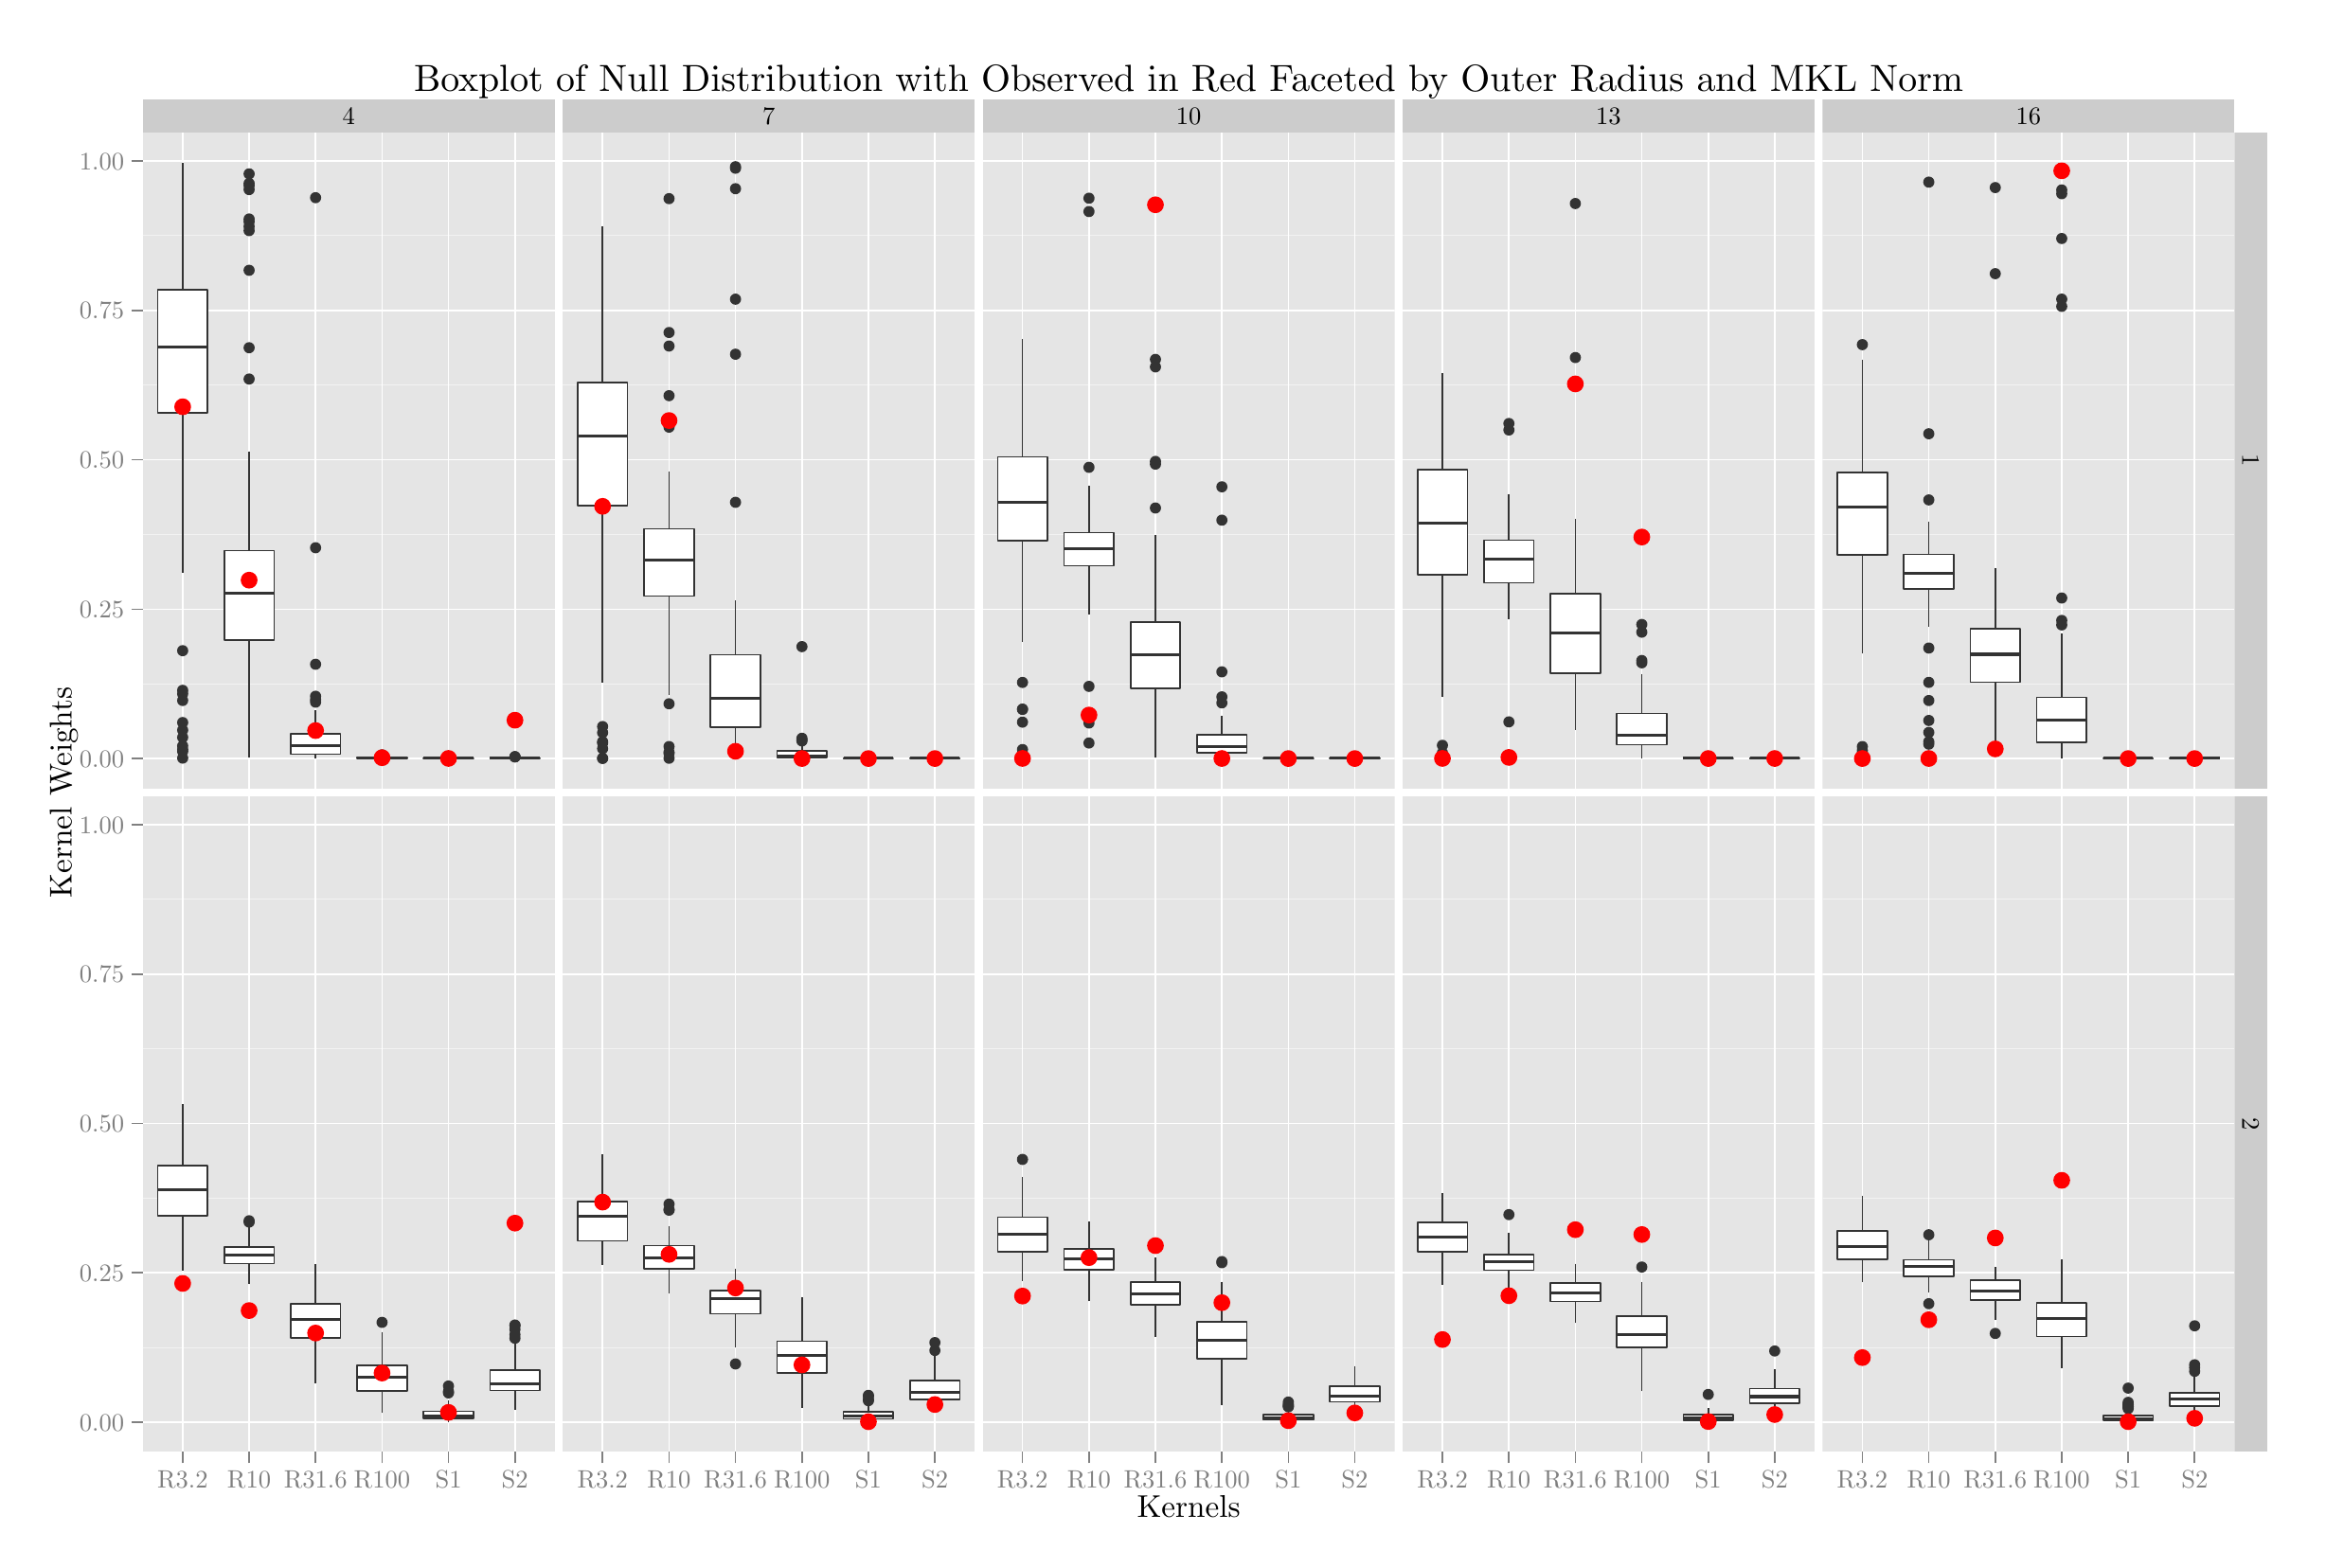
\begin{tikzpicture}[x=1pt,y=1pt]
\definecolor[named]{fillColor}{rgb}{1.00,1.00,1.00}
\path[use as bounding box,fill=fillColor,fill opacity=0.00] (0,0) rectangle (867.24,578.16);
\begin{scope}
\path[clip] (  0.00,  0.00) rectangle (867.24,578.16);
\definecolor[named]{drawColor}{rgb}{1.00,1.00,1.00}
\definecolor[named]{fillColor}{rgb}{1.00,1.00,1.00}

\path[draw=drawColor,line width= 0.6pt,line join=round,line cap=round,fill=fillColor] ( -0.00,  0.00) rectangle (867.24,578.16);
\end{scope}
\begin{scope}
\path[clip] ( 44.49,537.54) rectangle (201.69,550.17);
\definecolor[named]{fillColor}{rgb}{0.80,0.80,0.80}

\path[fill=fillColor] ( 44.49,537.54) rectangle (201.69,550.17);
\definecolor[named]{drawColor}{rgb}{0.00,0.00,0.00}

\node[text=drawColor,anchor=base,inner sep=0pt, outer sep=0pt, scale=  0.96] at (123.09,540.55) {4};
\end{scope}
\begin{scope}
\path[clip] (204.70,537.54) rectangle (361.91,550.17);
\definecolor[named]{fillColor}{rgb}{0.80,0.80,0.80}

\path[fill=fillColor] (204.70,537.54) rectangle (361.91,550.17);
\definecolor[named]{drawColor}{rgb}{0.00,0.00,0.00}

\node[text=drawColor,anchor=base,inner sep=0pt, outer sep=0pt, scale=  0.96] at (283.31,540.55) {7};
\end{scope}
\begin{scope}
\path[clip] (364.92,537.54) rectangle (522.13,550.17);
\definecolor[named]{fillColor}{rgb}{0.80,0.80,0.80}

\path[fill=fillColor] (364.92,537.54) rectangle (522.13,550.17);
\definecolor[named]{drawColor}{rgb}{0.00,0.00,0.00}

\node[text=drawColor,anchor=base,inner sep=0pt, outer sep=0pt, scale=  0.96] at (443.52,540.55) {10};
\end{scope}
\begin{scope}
\path[clip] (525.14,537.54) rectangle (682.34,550.17);
\definecolor[named]{fillColor}{rgb}{0.80,0.80,0.80}

\path[fill=fillColor] (525.14,537.54) rectangle (682.34,550.17);
\definecolor[named]{drawColor}{rgb}{0.00,0.00,0.00}

\node[text=drawColor,anchor=base,inner sep=0pt, outer sep=0pt, scale=  0.96] at (603.74,540.55) {13};
\end{scope}
\begin{scope}
\path[clip] (685.35,537.54) rectangle (842.56,550.17);
\definecolor[named]{fillColor}{rgb}{0.80,0.80,0.80}

\path[fill=fillColor] (685.35,537.54) rectangle (842.56,550.17);
\definecolor[named]{drawColor}{rgb}{0.00,0.00,0.00}

\node[text=drawColor,anchor=base,inner sep=0pt, outer sep=0pt, scale=  0.96] at (763.96,540.55) {16};
\end{scope}
\begin{scope}
\path[clip] ( 44.49,287.29) rectangle (201.69,537.54);
\definecolor[named]{fillColor}{rgb}{0.90,0.90,0.90}

\path[fill=fillColor] ( 44.49,287.29) rectangle (201.69,537.54);
\definecolor[named]{drawColor}{rgb}{0.95,0.95,0.95}

\path[draw=drawColor,line width= 0.3pt,line join=round] ( 44.49,327.17) --
	(201.69,327.17);

\path[draw=drawColor,line width= 0.3pt,line join=round] ( 44.49,384.18) --
	(201.69,384.18);

\path[draw=drawColor,line width= 0.3pt,line join=round] ( 44.49,441.20) --
	(201.69,441.20);

\path[draw=drawColor,line width= 0.3pt,line join=round] ( 44.49,498.21) --
	(201.69,498.21);
\definecolor[named]{drawColor}{rgb}{1.00,1.00,1.00}

\path[draw=drawColor,line width= 0.6pt,line join=round] ( 44.49,298.67) --
	(201.69,298.67);

\path[draw=drawColor,line width= 0.6pt,line join=round] ( 44.49,355.68) --
	(201.69,355.68);

\path[draw=drawColor,line width= 0.6pt,line join=round] ( 44.49,412.69) --
	(201.69,412.69);

\path[draw=drawColor,line width= 0.6pt,line join=round] ( 44.49,469.70) --
	(201.69,469.70);

\path[draw=drawColor,line width= 0.6pt,line join=round] ( 44.49,526.72) --
	(201.69,526.72);

\path[draw=drawColor,line width= 0.6pt,line join=round] ( 59.70,287.29) --
	( 59.70,537.54);

\path[draw=drawColor,line width= 0.6pt,line join=round] ( 85.05,287.29) --
	( 85.05,537.54);

\path[draw=drawColor,line width= 0.6pt,line join=round] (110.41,287.29) --
	(110.41,537.54);

\path[draw=drawColor,line width= 0.6pt,line join=round] (135.77,287.29) --
	(135.77,537.54);

\path[draw=drawColor,line width= 0.6pt,line join=round] (161.12,287.29) --
	(161.12,537.54);

\path[draw=drawColor,line width= 0.6pt,line join=round] (186.48,287.29) --
	(186.48,537.54);
\definecolor[named]{fillColor}{rgb}{0.20,0.20,0.20}

\path[fill=fillColor] ( 59.70,301.39) circle (  2.13);

\path[fill=fillColor] ( 59.70,320.83) circle (  2.13);

\path[fill=fillColor] ( 59.70,309.52) circle (  2.13);

\path[fill=fillColor] ( 59.70,312.41) circle (  2.13);

\path[fill=fillColor] ( 59.70,324.70) circle (  2.13);

\path[fill=fillColor] ( 59.70,303.50) circle (  2.13);

\path[fill=fillColor] ( 59.70,302.12) circle (  2.13);

\path[fill=fillColor] ( 59.70,323.35) circle (  2.13);

\path[fill=fillColor] ( 59.70,339.84) circle (  2.13);

\path[fill=fillColor] ( 59.70,306.75) circle (  2.13);

\path[fill=fillColor] ( 59.70,298.84) circle (  2.13);
\definecolor[named]{drawColor}{rgb}{0.20,0.20,0.20}

\path[draw=drawColor,line width= 0.6pt,line join=round,fill=fillColor] ( 59.70,477.67) -- ( 59.70,526.17);

\path[draw=drawColor,line width= 0.6pt,line join=round,fill=fillColor] ( 59.70,430.69) -- ( 59.70,369.63);
\definecolor[named]{fillColor}{rgb}{1.00,1.00,1.00}

\path[draw=drawColor,line width= 0.6pt,line join=round,line cap=round,fill=fillColor] ( 50.19,477.67) --
	( 50.19,430.69) --
	( 69.21,430.69) --
	( 69.21,477.67) --
	( 50.19,477.67) --
	cycle;
\definecolor[named]{fillColor}{rgb}{0.20,0.20,0.20}

\path[draw=drawColor,line width= 1.1pt,line join=round,fill=fillColor] ( 50.19,455.68) -- ( 69.21,455.68);

\path[fill=fillColor] ( 85.05,443.51) circle (  2.13);

\path[fill=fillColor] ( 85.05,503.57) circle (  2.13);

\path[fill=fillColor] ( 85.05,515.80) circle (  2.13);

\path[fill=fillColor] ( 85.05,504.58) circle (  2.13);

\path[fill=fillColor] ( 85.05,500.14) circle (  2.13);

\path[fill=fillColor] ( 85.05,521.79) circle (  2.13);

\path[fill=fillColor] ( 85.05,517.38) circle (  2.13);

\path[fill=fillColor] ( 85.05,501.71) circle (  2.13);

\path[fill=fillColor] ( 85.05,485.00) circle (  2.13);

\path[fill=fillColor] ( 85.05,518.17) circle (  2.13);

\path[fill=fillColor] ( 85.05,455.45) circle (  2.13);

\path[draw=drawColor,line width= 0.6pt,line join=round,fill=fillColor] ( 85.05,378.02) -- ( 85.05,415.89);

\path[draw=drawColor,line width= 0.6pt,line join=round,fill=fillColor] ( 85.05,343.91) -- ( 85.05,299.20);
\definecolor[named]{fillColor}{rgb}{1.00,1.00,1.00}

\path[draw=drawColor,line width= 0.6pt,line join=round,line cap=round,fill=fillColor] ( 75.55,378.02) --
	( 75.55,343.91) --
	( 94.56,343.91) --
	( 94.56,378.02) --
	( 75.55,378.02) --
	cycle;
\definecolor[named]{fillColor}{rgb}{0.20,0.20,0.20}

\path[draw=drawColor,line width= 1.1pt,line join=round,fill=fillColor] ( 75.55,361.64) -- ( 94.56,361.64);

\path[fill=fillColor] (110.41,320.19) circle (  2.13);

\path[fill=fillColor] (110.41,379.12) circle (  2.13);

\path[fill=fillColor] (110.41,322.45) circle (  2.13);

\path[fill=fillColor] (110.41,321.11) circle (  2.13);

\path[fill=fillColor] (110.41,512.71) circle (  2.13);

\path[fill=fillColor] (110.41,334.65) circle (  2.13);

\path[draw=drawColor,line width= 0.6pt,line join=round,fill=fillColor] (110.41,308.03) -- (110.41,317.12);

\path[draw=drawColor,line width= 0.6pt,line join=round,fill=fillColor] (110.41,300.34) -- (110.41,298.67);
\definecolor[named]{fillColor}{rgb}{1.00,1.00,1.00}

\path[draw=drawColor,line width= 0.6pt,line join=round,line cap=round,fill=fillColor] (100.90,308.03) --
	(100.90,300.34) --
	(119.92,300.34) --
	(119.92,308.03) --
	(100.90,308.03) --
	cycle;
\definecolor[named]{fillColor}{rgb}{0.20,0.20,0.20}

\path[draw=drawColor,line width= 1.1pt,line join=round,fill=fillColor] (100.90,303.42) -- (119.92,303.42);

\path[fill=fillColor] (135.77,299.50) circle (  2.13);

\path[fill=fillColor] (135.77,299.57) circle (  2.13);

\path[fill=fillColor] (135.77,299.61) circle (  2.13);

\path[fill=fillColor] (135.77,299.49) circle (  2.13);

\path[fill=fillColor] (135.77,300.09) circle (  2.13);

\path[draw=drawColor,line width= 0.6pt,line join=round,fill=fillColor] (135.77,299.02) -- (135.77,299.42);

\path[draw=drawColor,line width= 0.6pt,line join=round,fill=fillColor] (135.77,298.75) -- (135.77,298.67);
\definecolor[named]{fillColor}{rgb}{1.00,1.00,1.00}

\path[draw=drawColor,line width= 0.6pt,line join=round,line cap=round,fill=fillColor] (126.26,299.02) --
	(126.26,298.75) --
	(145.27,298.75) --
	(145.27,299.02) --
	(126.26,299.02) --
	cycle;
\definecolor[named]{fillColor}{rgb}{0.20,0.20,0.20}

\path[draw=drawColor,line width= 1.1pt,line join=round,fill=fillColor] (126.26,298.89) -- (145.27,298.89);

\path[fill=fillColor] (161.12,299.03) circle (  2.13);

\path[draw=drawColor,line width= 0.6pt,line join=round,fill=fillColor] (161.12,298.82) -- (161.12,298.97);

\path[draw=drawColor,line width= 0.6pt,line join=round,fill=fillColor] (161.12,298.69) -- (161.12,298.67);
\definecolor[named]{fillColor}{rgb}{1.00,1.00,1.00}

\path[draw=drawColor,line width= 0.6pt,line join=round,line cap=round,fill=fillColor] (151.61,298.82) --
	(151.61,298.69) --
	(170.63,298.69) --
	(170.63,298.82) --
	(151.61,298.82) --
	cycle;
\definecolor[named]{fillColor}{rgb}{0.20,0.20,0.20}

\path[draw=drawColor,line width= 1.1pt,line join=round,fill=fillColor] (151.61,298.75) -- (170.63,298.75);

\path[fill=fillColor] (186.48,299.30) circle (  2.13);

\path[fill=fillColor] (186.48,299.32) circle (  2.13);

\path[fill=fillColor] (186.48,299.41) circle (  2.13);

\path[draw=drawColor,line width= 0.6pt,line join=round,fill=fillColor] (186.48,298.92) -- (186.48,299.24);

\path[draw=drawColor,line width= 0.6pt,line join=round,fill=fillColor] (186.48,298.70) -- (186.48,298.67);
\definecolor[named]{fillColor}{rgb}{1.00,1.00,1.00}

\path[draw=drawColor,line width= 0.6pt,line join=round,line cap=round,fill=fillColor] (176.97,298.92) --
	(176.97,298.70) --
	(195.99,298.70) --
	(195.99,298.92) --
	(176.97,298.92) --
	cycle;
\definecolor[named]{fillColor}{rgb}{0.20,0.20,0.20}

\path[draw=drawColor,line width= 1.1pt,line join=round,fill=fillColor] (176.97,298.83) -- (195.99,298.83);
\definecolor[named]{fillColor}{rgb}{1.00,0.00,0.00}

\path[fill=fillColor] ( 59.70,432.91) circle (  3.20);

\path[fill=fillColor] ( 85.05,366.75) circle (  3.20);

\path[fill=fillColor] (110.41,309.35) circle (  3.20);

\path[fill=fillColor] (135.77,298.99) circle (  3.20);

\path[fill=fillColor] (161.12,298.72) circle (  3.20);

\path[fill=fillColor] (186.48,313.31) circle (  3.20);
\end{scope}
\begin{scope}
\path[clip] ( 44.49, 34.03) rectangle (201.69,284.28);
\definecolor[named]{fillColor}{rgb}{0.90,0.90,0.90}

\path[fill=fillColor] ( 44.49, 34.03) rectangle (201.69,284.28);
\definecolor[named]{drawColor}{rgb}{0.95,0.95,0.95}

\path[draw=drawColor,line width= 0.3pt,line join=round] ( 44.49, 73.91) --
	(201.69, 73.91);

\path[draw=drawColor,line width= 0.3pt,line join=round] ( 44.49,130.93) --
	(201.69,130.93);

\path[draw=drawColor,line width= 0.3pt,line join=round] ( 44.49,187.94) --
	(201.69,187.94);

\path[draw=drawColor,line width= 0.3pt,line join=round] ( 44.49,244.95) --
	(201.69,244.95);
\definecolor[named]{drawColor}{rgb}{1.00,1.00,1.00}

\path[draw=drawColor,line width= 0.6pt,line join=round] ( 44.49, 45.41) --
	(201.69, 45.41);

\path[draw=drawColor,line width= 0.6pt,line join=round] ( 44.49,102.42) --
	(201.69,102.42);

\path[draw=drawColor,line width= 0.6pt,line join=round] ( 44.49,159.43) --
	(201.69,159.43);

\path[draw=drawColor,line width= 0.6pt,line join=round] ( 44.49,216.44) --
	(201.69,216.44);

\path[draw=drawColor,line width= 0.6pt,line join=round] ( 44.49,273.46) --
	(201.69,273.46);

\path[draw=drawColor,line width= 0.6pt,line join=round] ( 59.70, 34.03) --
	( 59.70,284.28);

\path[draw=drawColor,line width= 0.6pt,line join=round] ( 85.05, 34.03) --
	( 85.05,284.28);

\path[draw=drawColor,line width= 0.6pt,line join=round] (110.41, 34.03) --
	(110.41,284.28);

\path[draw=drawColor,line width= 0.6pt,line join=round] (135.77, 34.03) --
	(135.77,284.28);

\path[draw=drawColor,line width= 0.6pt,line join=round] (161.12, 34.03) --
	(161.12,284.28);

\path[draw=drawColor,line width= 0.6pt,line join=round] (186.48, 34.03) --
	(186.48,284.28);
\definecolor[named]{drawColor}{rgb}{0.20,0.20,0.20}
\definecolor[named]{fillColor}{rgb}{0.20,0.20,0.20}

\path[draw=drawColor,line width= 0.6pt,line join=round,fill=fillColor] ( 59.70,143.26) -- ( 59.70,166.78);

\path[draw=drawColor,line width= 0.6pt,line join=round,fill=fillColor] ( 59.70,124.07) -- ( 59.70,103.19);
\definecolor[named]{fillColor}{rgb}{1.00,1.00,1.00}

\path[draw=drawColor,line width= 0.6pt,line join=round,line cap=round,fill=fillColor] ( 50.19,143.26) --
	( 50.19,124.07) --
	( 69.21,124.07) --
	( 69.21,143.26) --
	( 50.19,143.26) --
	cycle;
\definecolor[named]{fillColor}{rgb}{0.20,0.20,0.20}

\path[draw=drawColor,line width= 1.1pt,line join=round,fill=fillColor] ( 50.19,133.95) -- ( 69.21,133.95);

\path[fill=fillColor] ( 85.05,121.78) circle (  2.13);

\path[fill=fillColor] ( 85.05,122.28) circle (  2.13);

\path[draw=drawColor,line width= 0.6pt,line join=round,fill=fillColor] ( 85.05,112.19) -- ( 85.05,121.48);

\path[draw=drawColor,line width= 0.6pt,line join=round,fill=fillColor] ( 85.05,105.96) -- ( 85.05, 97.99);
\definecolor[named]{fillColor}{rgb}{1.00,1.00,1.00}

\path[draw=drawColor,line width= 0.6pt,line join=round,line cap=round,fill=fillColor] ( 75.55,112.19) --
	( 75.55,105.96) --
	( 94.56,105.96) --
	( 94.56,112.19) --
	( 75.55,112.19) --
	cycle;
\definecolor[named]{fillColor}{rgb}{0.20,0.20,0.20}

\path[draw=drawColor,line width= 1.1pt,line join=round,fill=fillColor] ( 75.55,109.29) -- ( 94.56,109.29);

\path[draw=drawColor,line width= 0.6pt,line join=round,fill=fillColor] (110.41, 90.46) -- (110.41,105.75);

\path[draw=drawColor,line width= 0.6pt,line join=round,fill=fillColor] (110.41, 77.48) -- (110.41, 60.37);
\definecolor[named]{fillColor}{rgb}{1.00,1.00,1.00}

\path[draw=drawColor,line width= 0.6pt,line join=round,line cap=round,fill=fillColor] (100.90, 90.46) --
	(100.90, 77.48) --
	(119.92, 77.48) --
	(119.92, 90.46) --
	(100.90, 90.46) --
	cycle;
\definecolor[named]{fillColor}{rgb}{0.20,0.20,0.20}

\path[draw=drawColor,line width= 1.1pt,line join=round,fill=fillColor] (100.90, 84.46) -- (119.92, 84.46);

\path[fill=fillColor] (135.77, 83.50) circle (  2.13);

\path[draw=drawColor,line width= 0.6pt,line join=round,fill=fillColor] (135.77, 67.15) -- (135.77, 79.90);

\path[draw=drawColor,line width= 0.6pt,line join=round,fill=fillColor] (135.77, 57.32) -- (135.77, 48.89);
\definecolor[named]{fillColor}{rgb}{1.00,1.00,1.00}

\path[draw=drawColor,line width= 0.6pt,line join=round,line cap=round,fill=fillColor] (126.26, 67.15) --
	(126.26, 57.32) --
	(145.27, 57.32) --
	(145.27, 67.15) --
	(126.26, 67.15) --
	cycle;
\definecolor[named]{fillColor}{rgb}{0.20,0.20,0.20}

\path[draw=drawColor,line width= 1.1pt,line join=round,fill=fillColor] (126.26, 62.69) -- (145.27, 62.69);

\path[fill=fillColor] (161.12, 59.21) circle (  2.13);

\path[fill=fillColor] (161.12, 56.58) circle (  2.13);

\path[fill=fillColor] (161.12, 57.09) circle (  2.13);

\path[draw=drawColor,line width= 0.6pt,line join=round,fill=fillColor] (161.12, 49.62) -- (161.12, 53.58);

\path[draw=drawColor,line width= 0.6pt,line join=round,fill=fillColor] (161.12, 46.75) -- (161.12, 45.54);
\definecolor[named]{fillColor}{rgb}{1.00,1.00,1.00}

\path[draw=drawColor,line width= 0.6pt,line join=round,line cap=round,fill=fillColor] (151.61, 49.62) --
	(151.61, 46.75) --
	(170.63, 46.75) --
	(170.63, 49.62) --
	(151.61, 49.62) --
	cycle;
\definecolor[named]{fillColor}{rgb}{0.20,0.20,0.20}

\path[draw=drawColor,line width= 1.1pt,line join=round,fill=fillColor] (151.61, 47.93) -- (170.63, 47.93);

\path[fill=fillColor] (186.48, 80.82) circle (  2.13);

\path[fill=fillColor] (186.48, 77.44) circle (  2.13);

\path[fill=fillColor] (186.48, 82.32) circle (  2.13);

\path[fill=fillColor] (186.48, 82.49) circle (  2.13);

\path[fill=fillColor] (186.48, 78.84) circle (  2.13);

\path[draw=drawColor,line width= 0.6pt,line join=round,fill=fillColor] (186.48, 65.40) -- (186.48, 76.86);

\path[draw=drawColor,line width= 0.6pt,line join=round,fill=fillColor] (186.48, 57.52) -- (186.48, 50.20);
\definecolor[named]{fillColor}{rgb}{1.00,1.00,1.00}

\path[draw=drawColor,line width= 0.6pt,line join=round,line cap=round,fill=fillColor] (176.97, 65.40) --
	(176.97, 57.52) --
	(195.99, 57.52) --
	(195.99, 65.40) --
	(176.97, 65.40) --
	cycle;
\definecolor[named]{fillColor}{rgb}{0.20,0.20,0.20}

\path[draw=drawColor,line width= 1.1pt,line join=round,fill=fillColor] (176.97, 59.91) -- (195.99, 59.91);
\definecolor[named]{fillColor}{rgb}{1.00,0.00,0.00}

\path[fill=fillColor] ( 59.70, 98.36) circle (  3.20);

\path[fill=fillColor] ( 85.05, 88.01) circle (  3.20);

\path[fill=fillColor] (110.41, 79.43) circle (  3.20);

\path[fill=fillColor] (135.77, 64.16) circle (  3.20);

\path[fill=fillColor] (161.12, 49.14) circle (  3.20);

\path[fill=fillColor] (186.48,121.38) circle (  3.20);
\end{scope}
\begin{scope}
\path[clip] (204.70,287.29) rectangle (361.91,537.54);
\definecolor[named]{fillColor}{rgb}{0.90,0.90,0.90}

\path[fill=fillColor] (204.70,287.29) rectangle (361.91,537.54);
\definecolor[named]{drawColor}{rgb}{0.95,0.95,0.95}

\path[draw=drawColor,line width= 0.3pt,line join=round] (204.70,327.17) --
	(361.91,327.17);

\path[draw=drawColor,line width= 0.3pt,line join=round] (204.70,384.18) --
	(361.91,384.18);

\path[draw=drawColor,line width= 0.3pt,line join=round] (204.70,441.20) --
	(361.91,441.20);

\path[draw=drawColor,line width= 0.3pt,line join=round] (204.70,498.21) --
	(361.91,498.21);
\definecolor[named]{drawColor}{rgb}{1.00,1.00,1.00}

\path[draw=drawColor,line width= 0.6pt,line join=round] (204.70,298.67) --
	(361.91,298.67);

\path[draw=drawColor,line width= 0.6pt,line join=round] (204.70,355.68) --
	(361.91,355.68);

\path[draw=drawColor,line width= 0.6pt,line join=round] (204.70,412.69) --
	(361.91,412.69);

\path[draw=drawColor,line width= 0.6pt,line join=round] (204.70,469.70) --
	(361.91,469.70);

\path[draw=drawColor,line width= 0.6pt,line join=round] (204.70,526.72) --
	(361.91,526.72);

\path[draw=drawColor,line width= 0.6pt,line join=round] (219.92,287.29) --
	(219.92,537.54);

\path[draw=drawColor,line width= 0.6pt,line join=round] (245.27,287.29) --
	(245.27,537.54);

\path[draw=drawColor,line width= 0.6pt,line join=round] (270.63,287.29) --
	(270.63,537.54);

\path[draw=drawColor,line width= 0.6pt,line join=round] (295.98,287.29) --
	(295.98,537.54);

\path[draw=drawColor,line width= 0.6pt,line join=round] (321.34,287.29) --
	(321.34,537.54);

\path[draw=drawColor,line width= 0.6pt,line join=round] (346.70,287.29) --
	(346.70,537.54);
\definecolor[named]{fillColor}{rgb}{0.20,0.20,0.20}

\path[fill=fillColor] (219.92,310.88) circle (  2.13);

\path[fill=fillColor] (219.92,305.11) circle (  2.13);

\path[fill=fillColor] (219.92,298.74) circle (  2.13);

\path[fill=fillColor] (219.92,302.43) circle (  2.13);

\path[fill=fillColor] (219.92,298.76) circle (  2.13);

\path[fill=fillColor] (219.92,304.61) circle (  2.13);

\path[fill=fillColor] (219.92,308.55) circle (  2.13);
\definecolor[named]{drawColor}{rgb}{0.20,0.20,0.20}

\path[draw=drawColor,line width= 0.6pt,line join=round,fill=fillColor] (219.92,442.18) -- (219.92,501.86);

\path[draw=drawColor,line width= 0.6pt,line join=round,fill=fillColor] (219.92,395.30) -- (219.92,327.80);
\definecolor[named]{fillColor}{rgb}{1.00,1.00,1.00}

\path[draw=drawColor,line width= 0.6pt,line join=round,line cap=round,fill=fillColor] (210.41,442.18) --
	(210.41,395.30) --
	(229.42,395.30) --
	(229.42,442.18) --
	(210.41,442.18) --
	cycle;
\definecolor[named]{fillColor}{rgb}{0.20,0.20,0.20}

\path[draw=drawColor,line width= 1.1pt,line join=round,fill=fillColor] (210.41,421.58) -- (229.42,421.58);

\path[fill=fillColor] (245.27,512.35) circle (  2.13);

\path[fill=fillColor] (245.27,456.09) circle (  2.13);

\path[fill=fillColor] (245.27,437.15) circle (  2.13);

\path[fill=fillColor] (245.27,461.26) circle (  2.13);

\path[fill=fillColor] (245.27,300.63) circle (  2.13);

\path[fill=fillColor] (245.27,425.13) circle (  2.13);

\path[fill=fillColor] (245.27,301.08) circle (  2.13);

\path[fill=fillColor] (245.27,319.57) circle (  2.13);

\path[fill=fillColor] (245.27,303.25) circle (  2.13);

\path[fill=fillColor] (245.27,298.78) circle (  2.13);

\path[draw=drawColor,line width= 0.6pt,line join=round,fill=fillColor] (245.27,386.32) -- (245.27,408.28);

\path[draw=drawColor,line width= 0.6pt,line join=round,fill=fillColor] (245.27,360.73) -- (245.27,322.89);
\definecolor[named]{fillColor}{rgb}{1.00,1.00,1.00}

\path[draw=drawColor,line width= 0.6pt,line join=round,line cap=round,fill=fillColor] (235.76,386.32) --
	(235.76,360.73) --
	(254.78,360.73) --
	(254.78,386.32) --
	(235.76,386.32) --
	cycle;
\definecolor[named]{fillColor}{rgb}{0.20,0.20,0.20}

\path[draw=drawColor,line width= 1.1pt,line join=round,fill=fillColor] (235.76,374.57) -- (254.78,374.57);

\path[fill=fillColor] (270.63,524.53) circle (  2.13);

\path[fill=fillColor] (270.63,396.46) circle (  2.13);

\path[fill=fillColor] (270.63,452.97) circle (  2.13);

\path[fill=fillColor] (270.63,523.95) circle (  2.13);

\path[fill=fillColor] (270.63,516.14) circle (  2.13);

\path[fill=fillColor] (270.63,473.98) circle (  2.13);

\path[draw=drawColor,line width= 0.6pt,line join=round,fill=fillColor] (270.63,338.31) -- (270.63,359.02);

\path[draw=drawColor,line width= 0.6pt,line join=round,fill=fillColor] (270.63,310.55) -- (270.63,298.70);
\definecolor[named]{fillColor}{rgb}{1.00,1.00,1.00}

\path[draw=drawColor,line width= 0.6pt,line join=round,line cap=round,fill=fillColor] (261.12,338.31) --
	(261.12,310.55) --
	(280.14,310.55) --
	(280.14,338.31) --
	(261.12,338.31) --
	cycle;
\definecolor[named]{fillColor}{rgb}{0.20,0.20,0.20}

\path[draw=drawColor,line width= 1.1pt,line join=round,fill=fillColor] (261.12,321.70) -- (280.14,321.70);

\path[fill=fillColor] (295.98,305.39) circle (  2.13);

\path[fill=fillColor] (295.98,306.41) circle (  2.13);

\path[fill=fillColor] (295.98,305.75) circle (  2.13);

\path[fill=fillColor] (295.98,341.38) circle (  2.13);

\path[draw=drawColor,line width= 0.6pt,line join=round,fill=fillColor] (295.98,301.49) -- (295.98,304.49);

\path[draw=drawColor,line width= 0.6pt,line join=round,fill=fillColor] (295.98,299.16) -- (295.98,298.68);
\definecolor[named]{fillColor}{rgb}{1.00,1.00,1.00}

\path[draw=drawColor,line width= 0.6pt,line join=round,line cap=round,fill=fillColor] (286.48,301.49) --
	(286.48,299.16) --
	(305.49,299.16) --
	(305.49,301.49) --
	(286.48,301.49) --
	cycle;
\definecolor[named]{fillColor}{rgb}{0.20,0.20,0.20}

\path[draw=drawColor,line width= 1.1pt,line join=round,fill=fillColor] (286.48,299.63) -- (305.49,299.63);

\path[draw=drawColor,line width= 0.6pt,line join=round,fill=fillColor] (321.34,298.81) -- (321.34,298.89);

\path[draw=drawColor,line width= 0.6pt,line join=round,fill=fillColor] (321.34,298.72) -- (321.34,298.67);
\definecolor[named]{fillColor}{rgb}{1.00,1.00,1.00}

\path[draw=drawColor,line width= 0.6pt,line join=round,line cap=round,fill=fillColor] (311.83,298.81) --
	(311.83,298.72) --
	(330.85,298.72) --
	(330.85,298.81) --
	(311.83,298.81) --
	cycle;
\definecolor[named]{fillColor}{rgb}{0.20,0.20,0.20}

\path[draw=drawColor,line width= 1.1pt,line join=round,fill=fillColor] (311.83,298.77) -- (330.85,298.77);

\path[fill=fillColor] (346.70,299.11) circle (  2.13);

\path[draw=drawColor,line width= 0.6pt,line join=round,fill=fillColor] (346.70,298.89) -- (346.70,299.02);

\path[draw=drawColor,line width= 0.6pt,line join=round,fill=fillColor] (346.70,298.77) -- (346.70,298.67);
\definecolor[named]{fillColor}{rgb}{1.00,1.00,1.00}

\path[draw=drawColor,line width= 0.6pt,line join=round,line cap=round,fill=fillColor] (337.19,298.89) --
	(337.19,298.77) --
	(356.20,298.77) --
	(356.20,298.89) --
	(337.19,298.89) --
	cycle;
\definecolor[named]{fillColor}{rgb}{0.20,0.20,0.20}

\path[draw=drawColor,line width= 1.1pt,line join=round,fill=fillColor] (337.19,298.84) -- (356.20,298.84);
\definecolor[named]{fillColor}{rgb}{1.00,0.00,0.00}

\path[fill=fillColor] (219.92,394.92) circle (  3.20);

\path[fill=fillColor] (245.27,427.67) circle (  3.20);

\path[fill=fillColor] (270.63,301.44) circle (  3.20);

\path[fill=fillColor] (295.98,298.68) circle (  3.20);

\path[fill=fillColor] (321.34,298.67) circle (  3.20);

\path[fill=fillColor] (346.70,298.67) circle (  3.20);
\end{scope}
\begin{scope}
\path[clip] (204.70, 34.03) rectangle (361.91,284.28);
\definecolor[named]{fillColor}{rgb}{0.90,0.90,0.90}

\path[fill=fillColor] (204.70, 34.03) rectangle (361.91,284.28);
\definecolor[named]{drawColor}{rgb}{0.95,0.95,0.95}

\path[draw=drawColor,line width= 0.3pt,line join=round] (204.70, 73.91) --
	(361.91, 73.91);

\path[draw=drawColor,line width= 0.3pt,line join=round] (204.70,130.93) --
	(361.91,130.93);

\path[draw=drawColor,line width= 0.3pt,line join=round] (204.70,187.94) --
	(361.91,187.94);

\path[draw=drawColor,line width= 0.3pt,line join=round] (204.70,244.95) --
	(361.91,244.95);
\definecolor[named]{drawColor}{rgb}{1.00,1.00,1.00}

\path[draw=drawColor,line width= 0.6pt,line join=round] (204.70, 45.41) --
	(361.91, 45.41);

\path[draw=drawColor,line width= 0.6pt,line join=round] (204.70,102.42) --
	(361.91,102.42);

\path[draw=drawColor,line width= 0.6pt,line join=round] (204.70,159.43) --
	(361.91,159.43);

\path[draw=drawColor,line width= 0.6pt,line join=round] (204.70,216.44) --
	(361.91,216.44);

\path[draw=drawColor,line width= 0.6pt,line join=round] (204.70,273.46) --
	(361.91,273.46);

\path[draw=drawColor,line width= 0.6pt,line join=round] (219.92, 34.03) --
	(219.92,284.28);

\path[draw=drawColor,line width= 0.6pt,line join=round] (245.27, 34.03) --
	(245.27,284.28);

\path[draw=drawColor,line width= 0.6pt,line join=round] (270.63, 34.03) --
	(270.63,284.28);

\path[draw=drawColor,line width= 0.6pt,line join=round] (295.98, 34.03) --
	(295.98,284.28);

\path[draw=drawColor,line width= 0.6pt,line join=round] (321.34, 34.03) --
	(321.34,284.28);

\path[draw=drawColor,line width= 0.6pt,line join=round] (346.70, 34.03) --
	(346.70,284.28);
\definecolor[named]{drawColor}{rgb}{0.20,0.20,0.20}
\definecolor[named]{fillColor}{rgb}{0.20,0.20,0.20}

\path[draw=drawColor,line width= 0.6pt,line join=round,fill=fillColor] (219.92,129.62) -- (219.92,147.65);

\path[draw=drawColor,line width= 0.6pt,line join=round,fill=fillColor] (219.92,114.63) -- (219.92,105.55);
\definecolor[named]{fillColor}{rgb}{1.00,1.00,1.00}

\path[draw=drawColor,line width= 0.6pt,line join=round,line cap=round,fill=fillColor] (210.41,129.62) --
	(210.41,114.63) --
	(229.42,114.63) --
	(229.42,129.62) --
	(210.41,129.62) --
	cycle;
\definecolor[named]{fillColor}{rgb}{0.20,0.20,0.20}

\path[draw=drawColor,line width= 1.1pt,line join=round,fill=fillColor] (210.41,124.05) -- (229.42,124.05);

\path[fill=fillColor] (245.27,128.65) circle (  2.13);

\path[fill=fillColor] (245.27,126.31) circle (  2.13);

\path[fill=fillColor] (245.27,126.56) circle (  2.13);

\path[draw=drawColor,line width= 0.6pt,line join=round,fill=fillColor] (245.27,112.84) -- (245.27,120.26);

\path[draw=drawColor,line width= 0.6pt,line join=round,fill=fillColor] (245.27,104.02) -- (245.27, 94.45);
\definecolor[named]{fillColor}{rgb}{1.00,1.00,1.00}

\path[draw=drawColor,line width= 0.6pt,line join=round,line cap=round,fill=fillColor] (235.76,112.84) --
	(235.76,104.02) --
	(254.78,104.02) --
	(254.78,112.84) --
	(235.76,112.84) --
	cycle;
\definecolor[named]{fillColor}{rgb}{0.20,0.20,0.20}

\path[draw=drawColor,line width= 1.1pt,line join=round,fill=fillColor] (235.76,108.24) -- (254.78,108.24);

\path[fill=fillColor] (270.63, 67.64) circle (  2.13);

\path[draw=drawColor,line width= 0.6pt,line join=round,fill=fillColor] (270.63, 95.56) -- (270.63,103.93);

\path[draw=drawColor,line width= 0.6pt,line join=round,fill=fillColor] (270.63, 86.79) -- (270.63, 73.82);
\definecolor[named]{fillColor}{rgb}{1.00,1.00,1.00}

\path[draw=drawColor,line width= 0.6pt,line join=round,line cap=round,fill=fillColor] (261.12, 95.56) --
	(261.12, 86.79) --
	(280.14, 86.79) --
	(280.14, 95.56) --
	(261.12, 95.56) --
	cycle;
\definecolor[named]{fillColor}{rgb}{0.20,0.20,0.20}

\path[draw=drawColor,line width= 1.1pt,line join=round,fill=fillColor] (261.12, 92.55) -- (280.14, 92.55);

\path[draw=drawColor,line width= 0.6pt,line join=round,fill=fillColor] (295.98, 76.27) -- (295.98, 93.15);

\path[draw=drawColor,line width= 0.6pt,line join=round,fill=fillColor] (295.98, 64.23) -- (295.98, 50.99);
\definecolor[named]{fillColor}{rgb}{1.00,1.00,1.00}

\path[draw=drawColor,line width= 0.6pt,line join=round,line cap=round,fill=fillColor] (286.48, 76.27) --
	(286.48, 64.23) --
	(305.49, 64.23) --
	(305.49, 76.27) --
	(286.48, 76.27) --
	cycle;
\definecolor[named]{fillColor}{rgb}{0.20,0.20,0.20}

\path[draw=drawColor,line width= 1.1pt,line join=round,fill=fillColor] (286.48, 70.75) -- (305.49, 70.75);

\path[fill=fillColor] (321.34, 55.65) circle (  2.13);

\path[fill=fillColor] (321.34, 54.04) circle (  2.13);

\path[fill=fillColor] (321.34, 53.61) circle (  2.13);

\path[fill=fillColor] (321.34, 55.33) circle (  2.13);

\path[draw=drawColor,line width= 0.6pt,line join=round,fill=fillColor] (321.34, 49.42) -- (321.34, 52.88);

\path[draw=drawColor,line width= 0.6pt,line join=round,fill=fillColor] (321.34, 46.68) -- (321.34, 45.44);
\definecolor[named]{fillColor}{rgb}{1.00,1.00,1.00}

\path[draw=drawColor,line width= 0.6pt,line join=round,line cap=round,fill=fillColor] (311.83, 49.42) --
	(311.83, 46.68) --
	(330.85, 46.68) --
	(330.85, 49.42) --
	(311.83, 49.42) --
	cycle;
\definecolor[named]{fillColor}{rgb}{0.20,0.20,0.20}

\path[draw=drawColor,line width= 1.1pt,line join=round,fill=fillColor] (311.83, 47.72) -- (330.85, 47.72);

\path[fill=fillColor] (346.70, 75.79) circle (  2.13);

\path[fill=fillColor] (346.70, 72.78) circle (  2.13);

\path[draw=drawColor,line width= 0.6pt,line join=round,fill=fillColor] (346.70, 61.33) -- (346.70, 71.75);

\path[draw=drawColor,line width= 0.6pt,line join=round,fill=fillColor] (346.70, 54.11) -- (346.70, 50.73);
\definecolor[named]{fillColor}{rgb}{1.00,1.00,1.00}

\path[draw=drawColor,line width= 0.6pt,line join=round,line cap=round,fill=fillColor] (337.19, 61.33) --
	(337.19, 54.11) --
	(356.20, 54.11) --
	(356.20, 61.33) --
	(337.19, 61.33) --
	cycle;
\definecolor[named]{fillColor}{rgb}{0.20,0.20,0.20}

\path[draw=drawColor,line width= 1.1pt,line join=round,fill=fillColor] (337.19, 56.88) -- (356.20, 56.88);
\definecolor[named]{fillColor}{rgb}{1.00,0.00,0.00}

\path[fill=fillColor] (219.92,129.40) circle (  3.20);

\path[fill=fillColor] (245.27,109.45) circle (  3.20);

\path[fill=fillColor] (270.63, 96.62) circle (  3.20);

\path[fill=fillColor] (295.98, 67.28) circle (  3.20);

\path[fill=fillColor] (321.34, 45.59) circle (  3.20);

\path[fill=fillColor] (346.70, 52.15) circle (  3.20);
\end{scope}
\begin{scope}
\path[clip] (364.92,287.29) rectangle (522.13,537.54);
\definecolor[named]{fillColor}{rgb}{0.90,0.90,0.90}

\path[fill=fillColor] (364.92,287.29) rectangle (522.13,537.54);
\definecolor[named]{drawColor}{rgb}{0.95,0.95,0.95}

\path[draw=drawColor,line width= 0.3pt,line join=round] (364.92,327.17) --
	(522.13,327.17);

\path[draw=drawColor,line width= 0.3pt,line join=round] (364.92,384.18) --
	(522.13,384.18);

\path[draw=drawColor,line width= 0.3pt,line join=round] (364.92,441.20) --
	(522.13,441.20);

\path[draw=drawColor,line width= 0.3pt,line join=round] (364.92,498.21) --
	(522.13,498.21);
\definecolor[named]{drawColor}{rgb}{1.00,1.00,1.00}

\path[draw=drawColor,line width= 0.6pt,line join=round] (364.92,298.67) --
	(522.13,298.67);

\path[draw=drawColor,line width= 0.6pt,line join=round] (364.92,355.68) --
	(522.13,355.68);

\path[draw=drawColor,line width= 0.6pt,line join=round] (364.92,412.69) --
	(522.13,412.69);

\path[draw=drawColor,line width= 0.6pt,line join=round] (364.92,469.70) --
	(522.13,469.70);

\path[draw=drawColor,line width= 0.6pt,line join=round] (364.92,526.72) --
	(522.13,526.72);

\path[draw=drawColor,line width= 0.6pt,line join=round] (380.13,287.29) --
	(380.13,537.54);

\path[draw=drawColor,line width= 0.6pt,line join=round] (405.49,287.29) --
	(405.49,537.54);

\path[draw=drawColor,line width= 0.6pt,line join=round] (430.85,287.29) --
	(430.85,537.54);

\path[draw=drawColor,line width= 0.6pt,line join=round] (456.20,287.29) --
	(456.20,537.54);

\path[draw=drawColor,line width= 0.6pt,line join=round] (481.56,287.29) --
	(481.56,537.54);

\path[draw=drawColor,line width= 0.6pt,line join=round] (506.91,287.29) --
	(506.91,537.54);
\definecolor[named]{fillColor}{rgb}{0.20,0.20,0.20}

\path[fill=fillColor] (380.13,312.56) circle (  2.13);

\path[fill=fillColor] (380.13,317.53) circle (  2.13);

\path[fill=fillColor] (380.13,299.78) circle (  2.13);

\path[fill=fillColor] (380.13,317.43) circle (  2.13);

\path[fill=fillColor] (380.13,299.84) circle (  2.13);

\path[fill=fillColor] (380.13,327.72) circle (  2.13);

\path[fill=fillColor] (380.13,302.10) circle (  2.13);
\definecolor[named]{drawColor}{rgb}{0.20,0.20,0.20}

\path[draw=drawColor,line width= 0.6pt,line join=round,fill=fillColor] (380.13,413.78) -- (380.13,458.80);

\path[draw=drawColor,line width= 0.6pt,line join=round,fill=fillColor] (380.13,381.86) -- (380.13,343.15);
\definecolor[named]{fillColor}{rgb}{1.00,1.00,1.00}

\path[draw=drawColor,line width= 0.6pt,line join=round,line cap=round,fill=fillColor] (370.63,413.78) --
	(370.63,381.86) --
	(389.64,381.86) --
	(389.64,413.78) --
	(370.63,413.78) --
	cycle;
\definecolor[named]{fillColor}{rgb}{0.20,0.20,0.20}

\path[draw=drawColor,line width= 1.1pt,line join=round,fill=fillColor] (370.63,396.55) -- (389.64,396.55);

\path[fill=fillColor] (405.49,512.51) circle (  2.13);

\path[fill=fillColor] (405.49,507.42) circle (  2.13);

\path[fill=fillColor] (405.49,304.60) circle (  2.13);

\path[fill=fillColor] (405.49,326.21) circle (  2.13);

\path[fill=fillColor] (405.49,312.23) circle (  2.13);

\path[fill=fillColor] (405.49,409.81) circle (  2.13);

\path[draw=drawColor,line width= 0.6pt,line join=round,fill=fillColor] (405.49,384.91) -- (405.49,402.82);

\path[draw=drawColor,line width= 0.6pt,line join=round,fill=fillColor] (405.49,372.25) -- (405.49,353.63);
\definecolor[named]{fillColor}{rgb}{1.00,1.00,1.00}

\path[draw=drawColor,line width= 0.6pt,line join=round,line cap=round,fill=fillColor] (395.98,384.91) --
	(395.98,372.25) --
	(415.00,372.25) --
	(415.00,384.91) --
	(395.98,384.91) --
	cycle;
\definecolor[named]{fillColor}{rgb}{0.20,0.20,0.20}

\path[draw=drawColor,line width= 1.1pt,line join=round,fill=fillColor] (395.98,378.69) -- (415.00,378.69);

\path[fill=fillColor] (430.85,448.14) circle (  2.13);

\path[fill=fillColor] (430.85,411.03) circle (  2.13);

\path[fill=fillColor] (430.85,394.29) circle (  2.13);

\path[fill=fillColor] (430.85,450.99) circle (  2.13);

\path[fill=fillColor] (430.85,412.07) circle (  2.13);

\path[draw=drawColor,line width= 0.6pt,line join=round,fill=fillColor] (430.85,350.84) -- (430.85,383.84);

\path[draw=drawColor,line width= 0.6pt,line join=round,fill=fillColor] (430.85,325.39) -- (430.85,298.93);
\definecolor[named]{fillColor}{rgb}{1.00,1.00,1.00}

\path[draw=drawColor,line width= 0.6pt,line join=round,line cap=round,fill=fillColor] (421.34,350.84) --
	(421.34,325.39) --
	(440.35,325.39) --
	(440.35,350.84) --
	(421.34,350.84) --
	cycle;
\definecolor[named]{fillColor}{rgb}{0.20,0.20,0.20}

\path[draw=drawColor,line width= 1.1pt,line join=round,fill=fillColor] (421.34,338.24) -- (440.35,338.24);

\path[fill=fillColor] (456.20,322.21) circle (  2.13);

\path[fill=fillColor] (456.20,389.65) circle (  2.13);

\path[fill=fillColor] (456.20,402.37) circle (  2.13);

\path[fill=fillColor] (456.20,331.76) circle (  2.13);

\path[fill=fillColor] (456.20,319.91) circle (  2.13);

\path[draw=drawColor,line width= 0.6pt,line join=round,fill=fillColor] (456.20,307.64) -- (456.20,315.06);

\path[draw=drawColor,line width= 0.6pt,line join=round,fill=fillColor] (456.20,301.00) -- (456.20,298.69);
\definecolor[named]{fillColor}{rgb}{1.00,1.00,1.00}

\path[draw=drawColor,line width= 0.6pt,line join=round,line cap=round,fill=fillColor] (446.69,307.64) --
	(446.69,301.00) --
	(465.71,301.00) --
	(465.71,307.64) --
	(446.69,307.64) --
	cycle;
\definecolor[named]{fillColor}{rgb}{0.20,0.20,0.20}

\path[draw=drawColor,line width= 1.1pt,line join=round,fill=fillColor] (446.69,303.09) -- (465.71,303.09);

\path[draw=drawColor,line width= 0.6pt,line join=round,fill=fillColor] (481.56,298.78) -- (481.56,298.87);

\path[draw=drawColor,line width= 0.6pt,line join=round,fill=fillColor] (481.56,298.71) -- (481.56,298.67);
\definecolor[named]{fillColor}{rgb}{1.00,1.00,1.00}

\path[draw=drawColor,line width= 0.6pt,line join=round,line cap=round,fill=fillColor] (472.05,298.78) --
	(472.05,298.71) --
	(491.07,298.71) --
	(491.07,298.78) --
	(472.05,298.78) --
	cycle;
\definecolor[named]{fillColor}{rgb}{0.20,0.20,0.20}

\path[draw=drawColor,line width= 1.1pt,line join=round,fill=fillColor] (472.05,298.74) -- (491.07,298.74);

\path[draw=drawColor,line width= 0.6pt,line join=round,fill=fillColor] (506.91,298.84) -- (506.91,298.97);

\path[draw=drawColor,line width= 0.6pt,line join=round,fill=fillColor] (506.91,298.74) -- (506.91,298.67);
\definecolor[named]{fillColor}{rgb}{1.00,1.00,1.00}

\path[draw=drawColor,line width= 0.6pt,line join=round,line cap=round,fill=fillColor] (497.40,298.84) --
	(497.40,298.74) --
	(516.42,298.74) --
	(516.42,298.84) --
	(497.40,298.84) --
	cycle;
\definecolor[named]{fillColor}{rgb}{0.20,0.20,0.20}

\path[draw=drawColor,line width= 1.1pt,line join=round,fill=fillColor] (497.40,298.80) -- (516.42,298.80);
\definecolor[named]{fillColor}{rgb}{1.00,0.00,0.00}

\path[fill=fillColor] (380.13,298.72) circle (  3.20);

\path[fill=fillColor] (405.49,315.27) circle (  3.20);

\path[fill=fillColor] (430.85,510.00) circle (  3.20);

\path[fill=fillColor] (456.20,298.70) circle (  3.20);

\path[fill=fillColor] (481.56,298.67) circle (  3.20);

\path[fill=fillColor] (506.91,298.67) circle (  3.20);
\end{scope}
\begin{scope}
\path[clip] (364.92, 34.03) rectangle (522.13,284.28);
\definecolor[named]{fillColor}{rgb}{0.90,0.90,0.90}

\path[fill=fillColor] (364.92, 34.03) rectangle (522.13,284.28);
\definecolor[named]{drawColor}{rgb}{0.95,0.95,0.95}

\path[draw=drawColor,line width= 0.3pt,line join=round] (364.92, 73.91) --
	(522.13, 73.91);

\path[draw=drawColor,line width= 0.3pt,line join=round] (364.92,130.93) --
	(522.13,130.93);

\path[draw=drawColor,line width= 0.3pt,line join=round] (364.92,187.94) --
	(522.13,187.94);

\path[draw=drawColor,line width= 0.3pt,line join=round] (364.92,244.95) --
	(522.13,244.95);
\definecolor[named]{drawColor}{rgb}{1.00,1.00,1.00}

\path[draw=drawColor,line width= 0.6pt,line join=round] (364.92, 45.41) --
	(522.13, 45.41);

\path[draw=drawColor,line width= 0.6pt,line join=round] (364.92,102.42) --
	(522.13,102.42);

\path[draw=drawColor,line width= 0.6pt,line join=round] (364.92,159.43) --
	(522.13,159.43);

\path[draw=drawColor,line width= 0.6pt,line join=round] (364.92,216.44) --
	(522.13,216.44);

\path[draw=drawColor,line width= 0.6pt,line join=round] (364.92,273.46) --
	(522.13,273.46);

\path[draw=drawColor,line width= 0.6pt,line join=round] (380.13, 34.03) --
	(380.13,284.28);

\path[draw=drawColor,line width= 0.6pt,line join=round] (405.49, 34.03) --
	(405.49,284.28);

\path[draw=drawColor,line width= 0.6pt,line join=round] (430.85, 34.03) --
	(430.85,284.28);

\path[draw=drawColor,line width= 0.6pt,line join=round] (456.20, 34.03) --
	(456.20,284.28);

\path[draw=drawColor,line width= 0.6pt,line join=round] (481.56, 34.03) --
	(481.56,284.28);

\path[draw=drawColor,line width= 0.6pt,line join=round] (506.91, 34.03) --
	(506.91,284.28);
\definecolor[named]{fillColor}{rgb}{0.20,0.20,0.20}

\path[fill=fillColor] (380.13,145.69) circle (  2.13);
\definecolor[named]{drawColor}{rgb}{0.20,0.20,0.20}

\path[draw=drawColor,line width= 0.6pt,line join=round,fill=fillColor] (380.13,123.62) -- (380.13,138.96);

\path[draw=drawColor,line width= 0.6pt,line join=round,fill=fillColor] (380.13,110.35) -- (380.13, 99.34);
\definecolor[named]{fillColor}{rgb}{1.00,1.00,1.00}

\path[draw=drawColor,line width= 0.6pt,line join=round,line cap=round,fill=fillColor] (370.63,123.62) --
	(370.63,110.35) --
	(389.64,110.35) --
	(389.64,123.62) --
	(370.63,123.62) --
	cycle;
\definecolor[named]{fillColor}{rgb}{0.20,0.20,0.20}

\path[draw=drawColor,line width= 1.1pt,line join=round,fill=fillColor] (370.63,117.07) -- (389.64,117.07);

\path[draw=drawColor,line width= 0.6pt,line join=round,fill=fillColor] (405.49,111.58) -- (405.49,121.90);

\path[draw=drawColor,line width= 0.6pt,line join=round,fill=fillColor] (405.49,103.51) -- (405.49, 91.56);
\definecolor[named]{fillColor}{rgb}{1.00,1.00,1.00}

\path[draw=drawColor,line width= 0.6pt,line join=round,line cap=round,fill=fillColor] (395.98,111.58) --
	(395.98,103.51) --
	(415.00,103.51) --
	(415.00,111.58) --
	(395.98,111.58) --
	cycle;
\definecolor[named]{fillColor}{rgb}{0.20,0.20,0.20}

\path[draw=drawColor,line width= 1.1pt,line join=round,fill=fillColor] (395.98,107.71) -- (415.00,107.71);

\path[draw=drawColor,line width= 0.6pt,line join=round,fill=fillColor] (430.85, 98.83) -- (430.85,108.28);

\path[draw=drawColor,line width= 0.6pt,line join=round,fill=fillColor] (430.85, 90.29) -- (430.85, 78.10);
\definecolor[named]{fillColor}{rgb}{1.00,1.00,1.00}

\path[draw=drawColor,line width= 0.6pt,line join=round,line cap=round,fill=fillColor] (421.34, 98.83) --
	(421.34, 90.29) --
	(440.35, 90.29) --
	(440.35, 98.83) --
	(421.34, 98.83) --
	cycle;
\definecolor[named]{fillColor}{rgb}{0.20,0.20,0.20}

\path[draw=drawColor,line width= 1.1pt,line join=round,fill=fillColor] (421.34, 94.48) -- (440.35, 94.48);

\path[fill=fillColor] (456.20,106.71) circle (  2.13);

\path[fill=fillColor] (456.20,106.27) circle (  2.13);

\path[draw=drawColor,line width= 0.6pt,line join=round,fill=fillColor] (456.20, 83.75) -- (456.20, 99.07);

\path[draw=drawColor,line width= 0.6pt,line join=round,fill=fillColor] (456.20, 69.72) -- (456.20, 51.86);
\definecolor[named]{fillColor}{rgb}{1.00,1.00,1.00}

\path[draw=drawColor,line width= 0.6pt,line join=round,line cap=round,fill=fillColor] (446.69, 83.75) --
	(446.69, 69.72) --
	(465.71, 69.72) --
	(465.71, 83.75) --
	(446.69, 83.75) --
	cycle;
\definecolor[named]{fillColor}{rgb}{0.20,0.20,0.20}

\path[draw=drawColor,line width= 1.1pt,line join=round,fill=fillColor] (446.69, 76.78) -- (465.71, 76.78);

\path[fill=fillColor] (481.56, 51.84) circle (  2.13);

\path[fill=fillColor] (481.56, 52.27) circle (  2.13);

\path[fill=fillColor] (481.56, 51.47) circle (  2.13);

\path[fill=fillColor] (481.56, 51.27) circle (  2.13);

\path[fill=fillColor] (481.56, 53.09) circle (  2.13);

\path[draw=drawColor,line width= 0.6pt,line join=round,fill=fillColor] (481.56, 48.28) -- (481.56, 51.13);

\path[draw=drawColor,line width= 0.6pt,line join=round,fill=fillColor] (481.56, 46.33) -- (481.56, 45.51);
\definecolor[named]{fillColor}{rgb}{1.00,1.00,1.00}

\path[draw=drawColor,line width= 0.6pt,line join=round,line cap=round,fill=fillColor] (472.05, 48.28) --
	(472.05, 46.33) --
	(491.07, 46.33) --
	(491.07, 48.28) --
	(472.05, 48.28) --
	cycle;
\definecolor[named]{fillColor}{rgb}{0.20,0.20,0.20}

\path[draw=drawColor,line width= 1.1pt,line join=round,fill=fillColor] (472.05, 47.11) -- (491.07, 47.11);

\path[draw=drawColor,line width= 0.6pt,line join=round,fill=fillColor] (506.91, 59.17) -- (506.91, 66.89);

\path[draw=drawColor,line width= 0.6pt,line join=round,fill=fillColor] (506.91, 53.13) -- (506.91, 48.59);
\definecolor[named]{fillColor}{rgb}{1.00,1.00,1.00}

\path[draw=drawColor,line width= 0.6pt,line join=round,line cap=round,fill=fillColor] (497.40, 59.17) --
	(497.40, 53.13) --
	(516.42, 53.13) --
	(516.42, 59.17) --
	(497.40, 59.17) --
	cycle;
\definecolor[named]{fillColor}{rgb}{0.20,0.20,0.20}

\path[draw=drawColor,line width= 1.1pt,line join=round,fill=fillColor] (497.40, 55.47) -- (516.42, 55.47);
\definecolor[named]{fillColor}{rgb}{1.00,0.00,0.00}

\path[fill=fillColor] (380.13, 93.55) circle (  3.20);

\path[fill=fillColor] (405.49,108.21) circle (  3.20);

\path[fill=fillColor] (430.85,112.79) circle (  3.20);

\path[fill=fillColor] (456.20, 91.01) circle (  3.20);

\path[fill=fillColor] (481.56, 45.99) circle (  3.20);

\path[fill=fillColor] (506.91, 48.94) circle (  3.20);
\end{scope}
\begin{scope}
\path[clip] (525.14,287.29) rectangle (682.34,537.54);
\definecolor[named]{fillColor}{rgb}{0.90,0.90,0.90}

\path[fill=fillColor] (525.14,287.29) rectangle (682.34,537.54);
\definecolor[named]{drawColor}{rgb}{0.95,0.95,0.95}

\path[draw=drawColor,line width= 0.3pt,line join=round] (525.14,327.17) --
	(682.34,327.17);

\path[draw=drawColor,line width= 0.3pt,line join=round] (525.14,384.18) --
	(682.34,384.18);

\path[draw=drawColor,line width= 0.3pt,line join=round] (525.14,441.20) --
	(682.34,441.20);

\path[draw=drawColor,line width= 0.3pt,line join=round] (525.14,498.21) --
	(682.34,498.21);
\definecolor[named]{drawColor}{rgb}{1.00,1.00,1.00}

\path[draw=drawColor,line width= 0.6pt,line join=round] (525.14,298.67) --
	(682.34,298.67);

\path[draw=drawColor,line width= 0.6pt,line join=round] (525.14,355.68) --
	(682.34,355.68);

\path[draw=drawColor,line width= 0.6pt,line join=round] (525.14,412.69) --
	(682.34,412.69);

\path[draw=drawColor,line width= 0.6pt,line join=round] (525.14,469.70) --
	(682.34,469.70);

\path[draw=drawColor,line width= 0.6pt,line join=round] (525.14,526.72) --
	(682.34,526.72);

\path[draw=drawColor,line width= 0.6pt,line join=round] (540.35,287.29) --
	(540.35,537.54);

\path[draw=drawColor,line width= 0.6pt,line join=round] (565.71,287.29) --
	(565.71,537.54);

\path[draw=drawColor,line width= 0.6pt,line join=round] (591.06,287.29) --
	(591.06,537.54);

\path[draw=drawColor,line width= 0.6pt,line join=round] (616.42,287.29) --
	(616.42,537.54);

\path[draw=drawColor,line width= 0.6pt,line join=round] (641.77,287.29) --
	(641.77,537.54);

\path[draw=drawColor,line width= 0.6pt,line join=round] (667.13,287.29) --
	(667.13,537.54);
\definecolor[named]{fillColor}{rgb}{0.20,0.20,0.20}

\path[fill=fillColor] (540.35,300.85) circle (  2.13);

\path[fill=fillColor] (540.35,303.72) circle (  2.13);
\definecolor[named]{drawColor}{rgb}{0.20,0.20,0.20}

\path[draw=drawColor,line width= 0.6pt,line join=round,fill=fillColor] (540.35,408.81) -- (540.35,445.64);

\path[draw=drawColor,line width= 0.6pt,line join=round,fill=fillColor] (540.35,368.78) -- (540.35,322.08);
\definecolor[named]{fillColor}{rgb}{1.00,1.00,1.00}

\path[draw=drawColor,line width= 0.6pt,line join=round,line cap=round,fill=fillColor] (530.84,408.81) --
	(530.84,368.78) --
	(549.86,368.78) --
	(549.86,408.81) --
	(530.84,408.81) --
	cycle;
\definecolor[named]{fillColor}{rgb}{0.20,0.20,0.20}

\path[draw=drawColor,line width= 1.1pt,line join=round,fill=fillColor] (530.84,388.67) -- (549.86,388.67);

\path[fill=fillColor] (565.71,312.67) circle (  2.13);

\path[fill=fillColor] (565.71,424.05) circle (  2.13);

\path[fill=fillColor] (565.71,426.54) circle (  2.13);

\path[draw=drawColor,line width= 0.6pt,line join=round,fill=fillColor] (565.71,382.06) -- (565.71,399.70);

\path[draw=drawColor,line width= 0.6pt,line join=round,fill=fillColor] (565.71,365.76) -- (565.71,351.72);
\definecolor[named]{fillColor}{rgb}{1.00,1.00,1.00}

\path[draw=drawColor,line width= 0.6pt,line join=round,line cap=round,fill=fillColor] (556.20,382.06) --
	(556.20,365.76) --
	(575.22,365.76) --
	(575.22,382.06) --
	(556.20,382.06) --
	cycle;
\definecolor[named]{fillColor}{rgb}{0.20,0.20,0.20}

\path[draw=drawColor,line width= 1.1pt,line join=round,fill=fillColor] (556.20,374.78) -- (575.22,374.78);

\path[fill=fillColor] (591.06,510.48) circle (  2.13);

\path[fill=fillColor] (591.06,451.70) circle (  2.13);

\path[draw=drawColor,line width= 0.6pt,line join=round,fill=fillColor] (591.06,361.70) -- (591.06,390.02);

\path[draw=drawColor,line width= 0.6pt,line join=round,fill=fillColor] (591.06,331.34) -- (591.06,309.71);
\definecolor[named]{fillColor}{rgb}{1.00,1.00,1.00}

\path[draw=drawColor,line width= 0.6pt,line join=round,line cap=round,fill=fillColor] (581.55,361.70) --
	(581.55,331.34) --
	(600.57,331.34) --
	(600.57,361.70) --
	(581.55,361.70) --
	cycle;
\definecolor[named]{fillColor}{rgb}{0.20,0.20,0.20}

\path[draw=drawColor,line width= 1.1pt,line join=round,fill=fillColor] (581.55,346.45) -- (600.57,346.45);

\path[fill=fillColor] (616.42,335.21) circle (  2.13);

\path[fill=fillColor] (616.42,346.90) circle (  2.13);

\path[fill=fillColor] (616.42,336.08) circle (  2.13);

\path[fill=fillColor] (616.42,349.84) circle (  2.13);

\path[draw=drawColor,line width= 0.6pt,line join=round,fill=fillColor] (616.42,315.92) -- (616.42,330.93);

\path[draw=drawColor,line width= 0.6pt,line join=round,fill=fillColor] (616.42,303.98) -- (616.42,298.70);
\definecolor[named]{fillColor}{rgb}{1.00,1.00,1.00}

\path[draw=drawColor,line width= 0.6pt,line join=round,line cap=round,fill=fillColor] (606.91,315.92) --
	(606.91,303.98) --
	(625.93,303.98) --
	(625.93,315.92) --
	(606.91,315.92) --
	cycle;
\definecolor[named]{fillColor}{rgb}{0.20,0.20,0.20}

\path[draw=drawColor,line width= 1.1pt,line join=round,fill=fillColor] (606.91,307.60) -- (625.93,307.60);

\path[fill=fillColor] (641.77,298.88) circle (  2.13);

\path[fill=fillColor] (641.77,298.90) circle (  2.13);

\path[fill=fillColor] (641.77,298.90) circle (  2.13);

\path[draw=drawColor,line width= 0.6pt,line join=round,fill=fillColor] (641.77,298.78) -- (641.77,298.86);

\path[draw=drawColor,line width= 0.6pt,line join=round,fill=fillColor] (641.77,298.72) -- (641.77,298.67);
\definecolor[named]{fillColor}{rgb}{1.00,1.00,1.00}

\path[draw=drawColor,line width= 0.6pt,line join=round,line cap=round,fill=fillColor] (632.27,298.78) --
	(632.27,298.72) --
	(651.28,298.72) --
	(651.28,298.78) --
	(632.27,298.78) --
	cycle;
\definecolor[named]{fillColor}{rgb}{0.20,0.20,0.20}

\path[draw=drawColor,line width= 1.1pt,line join=round,fill=fillColor] (632.27,298.74) -- (651.28,298.74);

\path[fill=fillColor] (667.13,299.06) circle (  2.13);

\path[fill=fillColor] (667.13,299.16) circle (  2.13);

\path[fill=fillColor] (667.13,298.99) circle (  2.13);

\path[fill=fillColor] (667.13,299.02) circle (  2.13);

\path[fill=fillColor] (667.13,299.12) circle (  2.13);

\path[fill=fillColor] (667.13,299.06) circle (  2.13);

\path[draw=drawColor,line width= 0.6pt,line join=round,fill=fillColor] (667.13,298.84) -- (667.13,298.95);

\path[draw=drawColor,line width= 0.6pt,line join=round,fill=fillColor] (667.13,298.76) -- (667.13,298.67);
\definecolor[named]{fillColor}{rgb}{1.00,1.00,1.00}

\path[draw=drawColor,line width= 0.6pt,line join=round,line cap=round,fill=fillColor] (657.62,298.84) --
	(657.62,298.76) --
	(676.64,298.76) --
	(676.64,298.84) --
	(657.62,298.84) --
	cycle;
\definecolor[named]{fillColor}{rgb}{0.20,0.20,0.20}

\path[draw=drawColor,line width= 1.1pt,line join=round,fill=fillColor] (657.62,298.79) -- (676.64,298.79);
\definecolor[named]{fillColor}{rgb}{1.00,0.00,0.00}

\path[fill=fillColor] (540.35,298.72) circle (  3.20);

\path[fill=fillColor] (565.71,299.11) circle (  3.20);

\path[fill=fillColor] (591.06,441.64) circle (  3.20);

\path[fill=fillColor] (616.42,383.20) circle (  3.20);

\path[fill=fillColor] (641.77,298.68) circle (  3.20);

\path[fill=fillColor] (667.13,298.69) circle (  3.20);
\end{scope}
\begin{scope}
\path[clip] (525.14, 34.03) rectangle (682.34,284.28);
\definecolor[named]{fillColor}{rgb}{0.90,0.90,0.90}

\path[fill=fillColor] (525.14, 34.03) rectangle (682.34,284.28);
\definecolor[named]{drawColor}{rgb}{0.95,0.95,0.95}

\path[draw=drawColor,line width= 0.3pt,line join=round] (525.14, 73.91) --
	(682.34, 73.91);

\path[draw=drawColor,line width= 0.3pt,line join=round] (525.14,130.93) --
	(682.34,130.93);

\path[draw=drawColor,line width= 0.3pt,line join=round] (525.14,187.94) --
	(682.34,187.94);

\path[draw=drawColor,line width= 0.3pt,line join=round] (525.14,244.95) --
	(682.34,244.95);
\definecolor[named]{drawColor}{rgb}{1.00,1.00,1.00}

\path[draw=drawColor,line width= 0.6pt,line join=round] (525.14, 45.41) --
	(682.34, 45.41);

\path[draw=drawColor,line width= 0.6pt,line join=round] (525.14,102.42) --
	(682.34,102.42);

\path[draw=drawColor,line width= 0.6pt,line join=round] (525.14,159.43) --
	(682.34,159.43);

\path[draw=drawColor,line width= 0.6pt,line join=round] (525.14,216.44) --
	(682.34,216.44);

\path[draw=drawColor,line width= 0.6pt,line join=round] (525.14,273.46) --
	(682.34,273.46);

\path[draw=drawColor,line width= 0.6pt,line join=round] (540.35, 34.03) --
	(540.35,284.28);

\path[draw=drawColor,line width= 0.6pt,line join=round] (565.71, 34.03) --
	(565.71,284.28);

\path[draw=drawColor,line width= 0.6pt,line join=round] (591.06, 34.03) --
	(591.06,284.28);

\path[draw=drawColor,line width= 0.6pt,line join=round] (616.42, 34.03) --
	(616.42,284.28);

\path[draw=drawColor,line width= 0.6pt,line join=round] (641.77, 34.03) --
	(641.77,284.28);

\path[draw=drawColor,line width= 0.6pt,line join=round] (667.13, 34.03) --
	(667.13,284.28);
\definecolor[named]{drawColor}{rgb}{0.20,0.20,0.20}
\definecolor[named]{fillColor}{rgb}{0.20,0.20,0.20}

\path[draw=drawColor,line width= 0.6pt,line join=round,fill=fillColor] (540.35,121.62) -- (540.35,132.78);

\path[draw=drawColor,line width= 0.6pt,line join=round,fill=fillColor] (540.35,110.53) -- (540.35, 97.97);
\definecolor[named]{fillColor}{rgb}{1.00,1.00,1.00}

\path[draw=drawColor,line width= 0.6pt,line join=round,line cap=round,fill=fillColor] (530.84,121.62) --
	(530.84,110.53) --
	(549.86,110.53) --
	(549.86,121.62) --
	(530.84,121.62) --
	cycle;
\definecolor[named]{fillColor}{rgb}{0.20,0.20,0.20}

\path[draw=drawColor,line width= 1.1pt,line join=round,fill=fillColor] (530.84,115.91) -- (549.86,115.91);

\path[fill=fillColor] (565.71, 94.21) circle (  2.13);

\path[fill=fillColor] (565.71,124.63) circle (  2.13);

\path[fill=fillColor] (565.71, 94.22) circle (  2.13);

\path[draw=drawColor,line width= 0.6pt,line join=round,fill=fillColor] (565.71,109.34) -- (565.71,117.74);

\path[draw=drawColor,line width= 0.6pt,line join=round,fill=fillColor] (565.71,103.40) -- (565.71, 96.39);
\definecolor[named]{fillColor}{rgb}{1.00,1.00,1.00}

\path[draw=drawColor,line width= 0.6pt,line join=round,line cap=round,fill=fillColor] (556.20,109.34) --
	(556.20,103.40) --
	(575.22,103.40) --
	(575.22,109.34) --
	(556.20,109.34) --
	cycle;
\definecolor[named]{fillColor}{rgb}{0.20,0.20,0.20}

\path[draw=drawColor,line width= 1.1pt,line join=round,fill=fillColor] (556.20,106.77) -- (575.22,106.77);

\path[draw=drawColor,line width= 0.6pt,line join=round,fill=fillColor] (591.06, 98.51) -- (591.06,105.88);

\path[draw=drawColor,line width= 0.6pt,line join=round,fill=fillColor] (591.06, 91.50) -- (591.06, 83.21);
\definecolor[named]{fillColor}{rgb}{1.00,1.00,1.00}

\path[draw=drawColor,line width= 0.6pt,line join=round,line cap=round,fill=fillColor] (581.55, 98.51) --
	(581.55, 91.50) --
	(600.57, 91.50) --
	(600.57, 98.51) --
	(581.55, 98.51) --
	cycle;
\definecolor[named]{fillColor}{rgb}{0.20,0.20,0.20}

\path[draw=drawColor,line width= 1.1pt,line join=round,fill=fillColor] (581.55, 94.77) -- (600.57, 94.77);

\path[fill=fillColor] (616.42,104.62) circle (  2.13);

\path[draw=drawColor,line width= 0.6pt,line join=round,fill=fillColor] (616.42, 85.81) -- (616.42, 98.92);

\path[draw=drawColor,line width= 0.6pt,line join=round,fill=fillColor] (616.42, 74.03) -- (616.42, 57.18);
\definecolor[named]{fillColor}{rgb}{1.00,1.00,1.00}

\path[draw=drawColor,line width= 0.6pt,line join=round,line cap=round,fill=fillColor] (606.91, 85.81) --
	(606.91, 74.03) --
	(625.93, 74.03) --
	(625.93, 85.81) --
	(606.91, 85.81) --
	cycle;
\definecolor[named]{fillColor}{rgb}{0.20,0.20,0.20}

\path[draw=drawColor,line width= 1.1pt,line join=round,fill=fillColor] (606.91, 78.91) -- (625.93, 78.91);

\path[fill=fillColor] (641.77, 56.00) circle (  2.13);

\path[draw=drawColor,line width= 0.6pt,line join=round,fill=fillColor] (641.77, 48.22) -- (641.77, 50.76);

\path[draw=drawColor,line width= 0.6pt,line join=round,fill=fillColor] (641.77, 46.25) -- (641.77, 45.42);
\definecolor[named]{fillColor}{rgb}{1.00,1.00,1.00}

\path[draw=drawColor,line width= 0.6pt,line join=round,line cap=round,fill=fillColor] (632.27, 48.22) --
	(632.27, 46.25) --
	(651.28, 46.25) --
	(651.28, 48.22) --
	(632.27, 48.22) --
	cycle;
\definecolor[named]{fillColor}{rgb}{0.20,0.20,0.20}

\path[draw=drawColor,line width= 1.1pt,line join=round,fill=fillColor] (632.27, 47.15) -- (651.28, 47.15);

\path[fill=fillColor] (667.13, 72.58) circle (  2.13);

\path[draw=drawColor,line width= 0.6pt,line join=round,fill=fillColor] (667.13, 58.19) -- (667.13, 65.59);

\path[draw=drawColor,line width= 0.6pt,line join=round,fill=fillColor] (667.13, 52.68) -- (667.13, 47.26);
\definecolor[named]{fillColor}{rgb}{1.00,1.00,1.00}

\path[draw=drawColor,line width= 0.6pt,line join=round,line cap=round,fill=fillColor] (657.62, 58.19) --
	(657.62, 52.68) --
	(676.64, 52.68) --
	(676.64, 58.19) --
	(657.62, 58.19) --
	cycle;
\definecolor[named]{fillColor}{rgb}{0.20,0.20,0.20}

\path[draw=drawColor,line width= 1.1pt,line join=round,fill=fillColor] (657.62, 55.17) -- (676.64, 55.17);
\definecolor[named]{fillColor}{rgb}{1.00,0.00,0.00}

\path[fill=fillColor] (540.35, 76.96) circle (  3.20);

\path[fill=fillColor] (565.71, 93.67) circle (  3.20);

\path[fill=fillColor] (591.06,118.87) circle (  3.20);

\path[fill=fillColor] (616.42,117.03) circle (  3.20);

\path[fill=fillColor] (641.77, 45.65) circle (  3.20);

\path[fill=fillColor] (667.13, 48.32) circle (  3.20);
\end{scope}
\begin{scope}
\path[clip] (685.35,287.29) rectangle (842.56,537.54);
\definecolor[named]{fillColor}{rgb}{0.90,0.90,0.90}

\path[fill=fillColor] (685.35,287.29) rectangle (842.56,537.54);
\definecolor[named]{drawColor}{rgb}{0.95,0.95,0.95}

\path[draw=drawColor,line width= 0.3pt,line join=round] (685.35,327.17) --
	(842.56,327.17);

\path[draw=drawColor,line width= 0.3pt,line join=round] (685.35,384.18) --
	(842.56,384.18);

\path[draw=drawColor,line width= 0.3pt,line join=round] (685.35,441.20) --
	(842.56,441.20);

\path[draw=drawColor,line width= 0.3pt,line join=round] (685.35,498.21) --
	(842.56,498.21);
\definecolor[named]{drawColor}{rgb}{1.00,1.00,1.00}

\path[draw=drawColor,line width= 0.6pt,line join=round] (685.35,298.67) --
	(842.56,298.67);

\path[draw=drawColor,line width= 0.6pt,line join=round] (685.35,355.68) --
	(842.56,355.68);

\path[draw=drawColor,line width= 0.6pt,line join=round] (685.35,412.69) --
	(842.56,412.69);

\path[draw=drawColor,line width= 0.6pt,line join=round] (685.35,469.70) --
	(842.56,469.70);

\path[draw=drawColor,line width= 0.6pt,line join=round] (685.35,526.72) --
	(842.56,526.72);

\path[draw=drawColor,line width= 0.6pt,line join=round] (700.57,287.29) --
	(700.57,537.54);

\path[draw=drawColor,line width= 0.6pt,line join=round] (725.92,287.29) --
	(725.92,537.54);

\path[draw=drawColor,line width= 0.6pt,line join=round] (751.28,287.29) --
	(751.28,537.54);

\path[draw=drawColor,line width= 0.6pt,line join=round] (776.64,287.29) --
	(776.64,537.54);

\path[draw=drawColor,line width= 0.6pt,line join=round] (801.99,287.29) --
	(801.99,537.54);

\path[draw=drawColor,line width= 0.6pt,line join=round] (827.35,287.29) --
	(827.35,537.54);
\definecolor[named]{fillColor}{rgb}{0.20,0.20,0.20}

\path[fill=fillColor] (700.57,300.53) circle (  2.13);

\path[fill=fillColor] (700.57,300.62) circle (  2.13);

\path[fill=fillColor] (700.57,298.74) circle (  2.13);

\path[fill=fillColor] (700.57,303.23) circle (  2.13);

\path[fill=fillColor] (700.57,301.76) circle (  2.13);

\path[fill=fillColor] (700.57,456.63) circle (  2.13);

\path[fill=fillColor] (700.57,299.64) circle (  2.13);

\path[fill=fillColor] (700.57,299.33) circle (  2.13);
\definecolor[named]{drawColor}{rgb}{0.20,0.20,0.20}

\path[draw=drawColor,line width= 0.6pt,line join=round,fill=fillColor] (700.57,407.75) -- (700.57,450.85);

\path[draw=drawColor,line width= 0.6pt,line join=round,fill=fillColor] (700.57,376.44) -- (700.57,338.65);
\definecolor[named]{fillColor}{rgb}{1.00,1.00,1.00}

\path[draw=drawColor,line width= 0.6pt,line join=round,line cap=round,fill=fillColor] (691.06,407.75) --
	(691.06,376.44) --
	(710.08,376.44) --
	(710.08,407.75) --
	(691.06,407.75) --
	cycle;
\definecolor[named]{fillColor}{rgb}{0.20,0.20,0.20}

\path[draw=drawColor,line width= 1.1pt,line join=round,fill=fillColor] (691.06,394.60) -- (710.08,394.60);

\path[fill=fillColor] (725.92,313.20) circle (  2.13);

\path[fill=fillColor] (725.92,299.03) circle (  2.13);

\path[fill=fillColor] (725.92,308.62) circle (  2.13);

\path[fill=fillColor] (725.92,422.62) circle (  2.13);

\path[fill=fillColor] (725.92,304.17) circle (  2.13);

\path[fill=fillColor] (725.92,327.74) circle (  2.13);

\path[fill=fillColor] (725.92,518.65) circle (  2.13);

\path[fill=fillColor] (725.92,320.81) circle (  2.13);

\path[fill=fillColor] (725.92,397.37) circle (  2.13);

\path[fill=fillColor] (725.92,305.12) circle (  2.13);

\path[fill=fillColor] (725.92,340.84) circle (  2.13);

\path[draw=drawColor,line width= 0.6pt,line join=round,fill=fillColor] (725.92,376.54) -- (725.92,388.96);

\path[draw=drawColor,line width= 0.6pt,line join=round,fill=fillColor] (725.92,363.44) -- (725.92,349.08);
\definecolor[named]{fillColor}{rgb}{1.00,1.00,1.00}

\path[draw=drawColor,line width= 0.6pt,line join=round,line cap=round,fill=fillColor] (716.42,376.54) --
	(716.42,363.44) --
	(735.43,363.44) --
	(735.43,376.54) --
	(716.42,376.54) --
	cycle;
\definecolor[named]{fillColor}{rgb}{0.20,0.20,0.20}

\path[draw=drawColor,line width= 1.1pt,line join=round,fill=fillColor] (716.42,369.50) -- (735.43,369.50);

\path[fill=fillColor] (751.28,483.72) circle (  2.13);

\path[fill=fillColor] (751.28,516.57) circle (  2.13);

\path[draw=drawColor,line width= 0.6pt,line join=round,fill=fillColor] (751.28,348.28) -- (751.28,371.47);

\path[draw=drawColor,line width= 0.6pt,line join=round,fill=fillColor] (751.28,327.80) -- (751.28,302.59);
\definecolor[named]{fillColor}{rgb}{1.00,1.00,1.00}

\path[draw=drawColor,line width= 0.6pt,line join=round,line cap=round,fill=fillColor] (741.77,348.28) --
	(741.77,327.80) --
	(760.79,327.80) --
	(760.79,348.28) --
	(741.77,348.28) --
	cycle;
\definecolor[named]{fillColor}{rgb}{0.20,0.20,0.20}

\path[draw=drawColor,line width= 1.1pt,line join=round,fill=fillColor] (741.77,338.46) -- (760.79,338.46);

\path[fill=fillColor] (776.64,514.22) circle (  2.13);

\path[fill=fillColor] (776.64,471.22) circle (  2.13);

\path[fill=fillColor] (776.64,473.99) circle (  2.13);

\path[fill=fillColor] (776.64,497.13) circle (  2.13);

\path[fill=fillColor] (776.64,349.67) circle (  2.13);

\path[fill=fillColor] (776.64,515.66) circle (  2.13);

\path[fill=fillColor] (776.64,351.38) circle (  2.13);

\path[fill=fillColor] (776.64,359.93) circle (  2.13);

\path[draw=drawColor,line width= 0.6pt,line join=round,fill=fillColor] (776.64,321.99) -- (776.64,346.51);

\path[draw=drawColor,line width= 0.6pt,line join=round,fill=fillColor] (776.64,304.84) -- (776.64,298.69);
\definecolor[named]{fillColor}{rgb}{1.00,1.00,1.00}

\path[draw=drawColor,line width= 0.6pt,line join=round,line cap=round,fill=fillColor] (767.13,321.99) --
	(767.13,304.84) --
	(786.14,304.84) --
	(786.14,321.99) --
	(767.13,321.99) --
	cycle;
\definecolor[named]{fillColor}{rgb}{0.20,0.20,0.20}

\path[draw=drawColor,line width= 1.1pt,line join=round,fill=fillColor] (767.13,313.19) -- (786.14,313.19);

\path[draw=drawColor,line width= 0.6pt,line join=round,fill=fillColor] (801.99,298.79) -- (801.99,298.88);

\path[draw=drawColor,line width= 0.6pt,line join=round,fill=fillColor] (801.99,298.71) -- (801.99,298.67);
\definecolor[named]{fillColor}{rgb}{1.00,1.00,1.00}

\path[draw=drawColor,line width= 0.6pt,line join=round,line cap=round,fill=fillColor] (792.48,298.79) --
	(792.48,298.71) --
	(811.50,298.71) --
	(811.50,298.79) --
	(792.48,298.79) --
	cycle;
\definecolor[named]{fillColor}{rgb}{0.20,0.20,0.20}

\path[draw=drawColor,line width= 1.1pt,line join=round,fill=fillColor] (792.48,298.75) -- (811.50,298.75);

\path[fill=fillColor] (827.35,299.06) circle (  2.13);

\path[fill=fillColor] (827.35,299.02) circle (  2.13);

\path[draw=drawColor,line width= 0.6pt,line join=round,fill=fillColor] (827.35,298.86) -- (827.35,298.99);

\path[draw=drawColor,line width= 0.6pt,line join=round,fill=fillColor] (827.35,298.76) -- (827.35,298.67);
\definecolor[named]{fillColor}{rgb}{1.00,1.00,1.00}

\path[draw=drawColor,line width= 0.6pt,line join=round,line cap=round,fill=fillColor] (817.84,298.86) --
	(817.84,298.76) --
	(836.86,298.76) --
	(836.86,298.86) --
	(817.84,298.86) --
	cycle;
\definecolor[named]{fillColor}{rgb}{0.20,0.20,0.20}

\path[draw=drawColor,line width= 1.1pt,line join=round,fill=fillColor] (817.84,298.81) -- (836.86,298.81);
\definecolor[named]{fillColor}{rgb}{1.00,0.00,0.00}

\path[fill=fillColor] (700.57,298.68) circle (  3.20);

\path[fill=fillColor] (725.92,298.70) circle (  3.20);

\path[fill=fillColor] (751.28,302.35) circle (  3.20);

\path[fill=fillColor] (776.64,522.97) circle (  3.20);

\path[fill=fillColor] (801.99,298.67) circle (  3.20);

\path[fill=fillColor] (827.35,298.67) circle (  3.20);
\end{scope}
\begin{scope}
\path[clip] (685.35, 34.03) rectangle (842.56,284.28);
\definecolor[named]{fillColor}{rgb}{0.90,0.90,0.90}

\path[fill=fillColor] (685.35, 34.03) rectangle (842.56,284.28);
\definecolor[named]{drawColor}{rgb}{0.95,0.95,0.95}

\path[draw=drawColor,line width= 0.3pt,line join=round] (685.35, 73.91) --
	(842.56, 73.91);

\path[draw=drawColor,line width= 0.3pt,line join=round] (685.35,130.93) --
	(842.56,130.93);

\path[draw=drawColor,line width= 0.3pt,line join=round] (685.35,187.94) --
	(842.56,187.94);

\path[draw=drawColor,line width= 0.3pt,line join=round] (685.35,244.95) --
	(842.56,244.95);
\definecolor[named]{drawColor}{rgb}{1.00,1.00,1.00}

\path[draw=drawColor,line width= 0.6pt,line join=round] (685.35, 45.41) --
	(842.56, 45.41);

\path[draw=drawColor,line width= 0.6pt,line join=round] (685.35,102.42) --
	(842.56,102.42);

\path[draw=drawColor,line width= 0.6pt,line join=round] (685.35,159.43) --
	(842.56,159.43);

\path[draw=drawColor,line width= 0.6pt,line join=round] (685.35,216.44) --
	(842.56,216.44);

\path[draw=drawColor,line width= 0.6pt,line join=round] (685.35,273.46) --
	(842.56,273.46);

\path[draw=drawColor,line width= 0.6pt,line join=round] (700.57, 34.03) --
	(700.57,284.28);

\path[draw=drawColor,line width= 0.6pt,line join=round] (725.92, 34.03) --
	(725.92,284.28);

\path[draw=drawColor,line width= 0.6pt,line join=round] (751.28, 34.03) --
	(751.28,284.28);

\path[draw=drawColor,line width= 0.6pt,line join=round] (776.64, 34.03) --
	(776.64,284.28);

\path[draw=drawColor,line width= 0.6pt,line join=round] (801.99, 34.03) --
	(801.99,284.28);

\path[draw=drawColor,line width= 0.6pt,line join=round] (827.35, 34.03) --
	(827.35,284.28);
\definecolor[named]{drawColor}{rgb}{0.20,0.20,0.20}
\definecolor[named]{fillColor}{rgb}{0.20,0.20,0.20}

\path[draw=drawColor,line width= 0.6pt,line join=round,fill=fillColor] (700.57,118.31) -- (700.57,131.72);

\path[draw=drawColor,line width= 0.6pt,line join=round,fill=fillColor] (700.57,107.65) -- (700.57, 98.71);
\definecolor[named]{fillColor}{rgb}{1.00,1.00,1.00}

\path[draw=drawColor,line width= 0.6pt,line join=round,line cap=round,fill=fillColor] (691.06,118.31) --
	(691.06,107.65) --
	(710.08,107.65) --
	(710.08,118.31) --
	(691.06,118.31) --
	cycle;
\definecolor[named]{fillColor}{rgb}{0.20,0.20,0.20}

\path[draw=drawColor,line width= 1.1pt,line join=round,fill=fillColor] (691.06,112.41) -- (710.08,112.41);

\path[fill=fillColor] (725.92,116.94) circle (  2.13);

\path[fill=fillColor] (725.92, 90.63) circle (  2.13);

\path[draw=drawColor,line width= 0.6pt,line join=round,fill=fillColor] (725.92,107.34) -- (725.92,115.12);

\path[draw=drawColor,line width= 0.6pt,line join=round,fill=fillColor] (725.92,101.17) -- (725.92, 94.91);
\definecolor[named]{fillColor}{rgb}{1.00,1.00,1.00}

\path[draw=drawColor,line width= 0.6pt,line join=round,line cap=round,fill=fillColor] (716.42,107.34) --
	(716.42,101.17) --
	(735.43,101.17) --
	(735.43,107.34) --
	(716.42,107.34) --
	cycle;
\definecolor[named]{fillColor}{rgb}{0.20,0.20,0.20}

\path[draw=drawColor,line width= 1.1pt,line join=round,fill=fillColor] (716.42,104.74) -- (735.43,104.74);

\path[fill=fillColor] (751.28, 79.28) circle (  2.13);

\path[draw=drawColor,line width= 0.6pt,line join=round,fill=fillColor] (751.28, 99.70) -- (751.28,104.50);

\path[draw=drawColor,line width= 0.6pt,line join=round,fill=fillColor] (751.28, 91.96) -- (751.28, 84.44);
\definecolor[named]{fillColor}{rgb}{1.00,1.00,1.00}

\path[draw=drawColor,line width= 0.6pt,line join=round,line cap=round,fill=fillColor] (741.77, 99.70) --
	(741.77, 91.96) --
	(760.79, 91.96) --
	(760.79, 99.70) --
	(741.77, 99.70) --
	cycle;
\definecolor[named]{fillColor}{rgb}{0.20,0.20,0.20}

\path[draw=drawColor,line width= 1.1pt,line join=round,fill=fillColor] (741.77, 95.43) -- (760.79, 95.43);

\path[draw=drawColor,line width= 0.6pt,line join=round,fill=fillColor] (776.64, 90.99) -- (776.64,107.47);

\path[draw=drawColor,line width= 0.6pt,line join=round,fill=fillColor] (776.64, 78.06) -- (776.64, 65.95);
\definecolor[named]{fillColor}{rgb}{1.00,1.00,1.00}

\path[draw=drawColor,line width= 0.6pt,line join=round,line cap=round,fill=fillColor] (767.13, 90.99) --
	(767.13, 78.06) --
	(786.14, 78.06) --
	(786.14, 90.99) --
	(767.13, 90.99) --
	cycle;
\definecolor[named]{fillColor}{rgb}{0.20,0.20,0.20}

\path[draw=drawColor,line width= 1.1pt,line join=round,fill=fillColor] (767.13, 85.08) -- (786.14, 85.08);

\path[fill=fillColor] (801.99, 51.27) circle (  2.13);

\path[fill=fillColor] (801.99, 52.98) circle (  2.13);

\path[fill=fillColor] (801.99, 52.28) circle (  2.13);

\path[fill=fillColor] (801.99, 50.59) circle (  2.13);

\path[fill=fillColor] (801.99, 51.17) circle (  2.13);

\path[fill=fillColor] (801.99, 51.46) circle (  2.13);

\path[fill=fillColor] (801.99, 52.16) circle (  2.13);

\path[fill=fillColor] (801.99, 51.93) circle (  2.13);

\path[fill=fillColor] (801.99, 58.41) circle (  2.13);

\path[draw=drawColor,line width= 0.6pt,line join=round,fill=fillColor] (801.99, 47.90) -- (801.99, 49.87);

\path[draw=drawColor,line width= 0.6pt,line join=round,fill=fillColor] (801.99, 46.15) -- (801.99, 45.44);
\definecolor[named]{fillColor}{rgb}{1.00,1.00,1.00}

\path[draw=drawColor,line width= 0.6pt,line join=round,line cap=round,fill=fillColor] (792.48, 47.90) --
	(792.48, 46.15) --
	(811.50, 46.15) --
	(811.50, 47.90) --
	(792.48, 47.90) --
	cycle;
\definecolor[named]{fillColor}{rgb}{0.20,0.20,0.20}

\path[draw=drawColor,line width= 1.1pt,line join=round,fill=fillColor] (792.48, 46.84) -- (811.50, 46.84);

\path[fill=fillColor] (827.35, 66.20) circle (  2.13);

\path[fill=fillColor] (827.35, 67.33) circle (  2.13);

\path[fill=fillColor] (827.35, 64.83) circle (  2.13);

\path[fill=fillColor] (827.35, 82.18) circle (  2.13);

\path[draw=drawColor,line width= 0.6pt,line join=round,fill=fillColor] (827.35, 56.56) -- (827.35, 63.80);

\path[draw=drawColor,line width= 0.6pt,line join=round,fill=fillColor] (827.35, 51.50) -- (827.35, 48.02);
\definecolor[named]{fillColor}{rgb}{1.00,1.00,1.00}

\path[draw=drawColor,line width= 0.6pt,line join=round,line cap=round,fill=fillColor] (817.84, 56.56) --
	(817.84, 51.50) --
	(836.86, 51.50) --
	(836.86, 56.56) --
	(817.84, 56.56) --
	cycle;
\definecolor[named]{fillColor}{rgb}{0.20,0.20,0.20}

\path[draw=drawColor,line width= 1.1pt,line join=round,fill=fillColor] (817.84, 54.16) -- (836.86, 54.16);
\definecolor[named]{fillColor}{rgb}{1.00,0.00,0.00}

\path[fill=fillColor] (700.57, 70.06) circle (  3.20);

\path[fill=fillColor] (725.92, 84.50) circle (  3.20);

\path[fill=fillColor] (751.28,115.71) circle (  3.20);

\path[fill=fillColor] (776.64,137.71) circle (  3.20);

\path[fill=fillColor] (801.99, 45.61) circle (  3.20);

\path[fill=fillColor] (827.35, 46.89) circle (  3.20);
\end{scope}
\begin{scope}
\path[clip] (  0.00,  0.00) rectangle (867.24,578.16);
\definecolor[named]{drawColor}{rgb}{0.50,0.50,0.50}

\node[text=drawColor,anchor=base east,inner sep=0pt, outer sep=0pt, scale=  0.96] at ( 37.37,295.36) {0.00};

\node[text=drawColor,anchor=base east,inner sep=0pt, outer sep=0pt, scale=  0.96] at ( 37.37,352.37) {0.25};

\node[text=drawColor,anchor=base east,inner sep=0pt, outer sep=0pt, scale=  0.96] at ( 37.37,409.38) {0.50};

\node[text=drawColor,anchor=base east,inner sep=0pt, outer sep=0pt, scale=  0.96] at ( 37.37,466.40) {0.75};

\node[text=drawColor,anchor=base east,inner sep=0pt, outer sep=0pt, scale=  0.96] at ( 37.37,523.41) {1.00};
\end{scope}
\begin{scope}
\path[clip] (  0.00,  0.00) rectangle (867.24,578.16);
\definecolor[named]{drawColor}{rgb}{0.50,0.50,0.50}

\path[draw=drawColor,line width= 0.6pt,line join=round] ( 40.22,298.67) --
	( 44.49,298.67);

\path[draw=drawColor,line width= 0.6pt,line join=round] ( 40.22,355.68) --
	( 44.49,355.68);

\path[draw=drawColor,line width= 0.6pt,line join=round] ( 40.22,412.69) --
	( 44.49,412.69);

\path[draw=drawColor,line width= 0.6pt,line join=round] ( 40.22,469.70) --
	( 44.49,469.70);

\path[draw=drawColor,line width= 0.6pt,line join=round] ( 40.22,526.72) --
	( 44.49,526.72);
\end{scope}
\begin{scope}
\path[clip] (  0.00,  0.00) rectangle (867.24,578.16);
\definecolor[named]{drawColor}{rgb}{0.50,0.50,0.50}

\node[text=drawColor,anchor=base east,inner sep=0pt, outer sep=0pt, scale=  0.96] at ( 37.37, 42.10) {0.00};

\node[text=drawColor,anchor=base east,inner sep=0pt, outer sep=0pt, scale=  0.96] at ( 37.37, 99.11) {0.25};

\node[text=drawColor,anchor=base east,inner sep=0pt, outer sep=0pt, scale=  0.96] at ( 37.37,156.13) {0.50};

\node[text=drawColor,anchor=base east,inner sep=0pt, outer sep=0pt, scale=  0.96] at ( 37.37,213.14) {0.75};

\node[text=drawColor,anchor=base east,inner sep=0pt, outer sep=0pt, scale=  0.96] at ( 37.37,270.15) {1.00};
\end{scope}
\begin{scope}
\path[clip] (  0.00,  0.00) rectangle (867.24,578.16);
\definecolor[named]{drawColor}{rgb}{0.50,0.50,0.50}

\path[draw=drawColor,line width= 0.6pt,line join=round] ( 40.22, 45.41) --
	( 44.49, 45.41);

\path[draw=drawColor,line width= 0.6pt,line join=round] ( 40.22,102.42) --
	( 44.49,102.42);

\path[draw=drawColor,line width= 0.6pt,line join=round] ( 40.22,159.43) --
	( 44.49,159.43);

\path[draw=drawColor,line width= 0.6pt,line join=round] ( 40.22,216.44) --
	( 44.49,216.44);

\path[draw=drawColor,line width= 0.6pt,line join=round] ( 40.22,273.46) --
	( 44.49,273.46);
\end{scope}
\begin{scope}
\path[clip] (842.56,287.29) rectangle (855.19,537.54);
\definecolor[named]{fillColor}{rgb}{0.80,0.80,0.80}

\path[fill=fillColor] (842.56,287.29) rectangle (855.19,537.54);
\definecolor[named]{drawColor}{rgb}{0.00,0.00,0.00}

\node[text=drawColor,rotate=270.00,anchor=base,inner sep=0pt, outer sep=0pt, scale=  0.96] at (845.57,412.42) {1};
\end{scope}
\begin{scope}
\path[clip] (842.56, 34.03) rectangle (855.19,284.28);
\definecolor[named]{fillColor}{rgb}{0.80,0.80,0.80}

\path[fill=fillColor] (842.56, 34.03) rectangle (855.19,284.28);
\definecolor[named]{drawColor}{rgb}{0.00,0.00,0.00}

\node[text=drawColor,rotate=270.00,anchor=base,inner sep=0pt, outer sep=0pt, scale=  0.96] at (845.57,159.16) {2};
\end{scope}
\begin{scope}
\path[clip] (  0.00,  0.00) rectangle (867.24,578.16);
\definecolor[named]{drawColor}{rgb}{0.50,0.50,0.50}

\path[draw=drawColor,line width= 0.6pt,line join=round] ( 59.70, 29.77) --
	( 59.70, 34.03);

\path[draw=drawColor,line width= 0.6pt,line join=round] ( 85.05, 29.77) --
	( 85.05, 34.03);

\path[draw=drawColor,line width= 0.6pt,line join=round] (110.41, 29.77) --
	(110.41, 34.03);

\path[draw=drawColor,line width= 0.6pt,line join=round] (135.77, 29.77) --
	(135.77, 34.03);

\path[draw=drawColor,line width= 0.6pt,line join=round] (161.12, 29.77) --
	(161.12, 34.03);

\path[draw=drawColor,line width= 0.6pt,line join=round] (186.48, 29.77) --
	(186.48, 34.03);
\end{scope}
\begin{scope}
\path[clip] (  0.00,  0.00) rectangle (867.24,578.16);
\definecolor[named]{drawColor}{rgb}{0.50,0.50,0.50}

\node[text=drawColor,anchor=base,inner sep=0pt, outer sep=0pt, scale=  0.96] at ( 59.70, 20.31) {R3.2};

\node[text=drawColor,anchor=base,inner sep=0pt, outer sep=0pt, scale=  0.96] at ( 85.05, 20.31) {R10};

\node[text=drawColor,anchor=base,inner sep=0pt, outer sep=0pt, scale=  0.96] at (110.41, 20.31) {R31.6};

\node[text=drawColor,anchor=base,inner sep=0pt, outer sep=0pt, scale=  0.96] at (135.77, 20.31) {R100};

\node[text=drawColor,anchor=base,inner sep=0pt, outer sep=0pt, scale=  0.96] at (161.12, 20.31) {S1};

\node[text=drawColor,anchor=base,inner sep=0pt, outer sep=0pt, scale=  0.96] at (186.48, 20.31) {S2};
\end{scope}
\begin{scope}
\path[clip] (  0.00,  0.00) rectangle (867.24,578.16);
\definecolor[named]{drawColor}{rgb}{0.50,0.50,0.50}

\path[draw=drawColor,line width= 0.6pt,line join=round] (219.92, 29.77) --
	(219.92, 34.03);

\path[draw=drawColor,line width= 0.6pt,line join=round] (245.27, 29.77) --
	(245.27, 34.03);

\path[draw=drawColor,line width= 0.6pt,line join=round] (270.63, 29.77) --
	(270.63, 34.03);

\path[draw=drawColor,line width= 0.6pt,line join=round] (295.98, 29.77) --
	(295.98, 34.03);

\path[draw=drawColor,line width= 0.6pt,line join=round] (321.34, 29.77) --
	(321.34, 34.03);

\path[draw=drawColor,line width= 0.6pt,line join=round] (346.70, 29.77) --
	(346.70, 34.03);
\end{scope}
\begin{scope}
\path[clip] (  0.00,  0.00) rectangle (867.24,578.16);
\definecolor[named]{drawColor}{rgb}{0.50,0.50,0.50}

\node[text=drawColor,anchor=base,inner sep=0pt, outer sep=0pt, scale=  0.96] at (219.92, 20.31) {R3.2};

\node[text=drawColor,anchor=base,inner sep=0pt, outer sep=0pt, scale=  0.96] at (245.27, 20.31) {R10};

\node[text=drawColor,anchor=base,inner sep=0pt, outer sep=0pt, scale=  0.96] at (270.63, 20.31) {R31.6};

\node[text=drawColor,anchor=base,inner sep=0pt, outer sep=0pt, scale=  0.96] at (295.98, 20.31) {R100};

\node[text=drawColor,anchor=base,inner sep=0pt, outer sep=0pt, scale=  0.96] at (321.34, 20.31) {S1};

\node[text=drawColor,anchor=base,inner sep=0pt, outer sep=0pt, scale=  0.96] at (346.70, 20.31) {S2};
\end{scope}
\begin{scope}
\path[clip] (  0.00,  0.00) rectangle (867.24,578.16);
\definecolor[named]{drawColor}{rgb}{0.50,0.50,0.50}

\path[draw=drawColor,line width= 0.6pt,line join=round] (380.13, 29.77) --
	(380.13, 34.03);

\path[draw=drawColor,line width= 0.6pt,line join=round] (405.49, 29.77) --
	(405.49, 34.03);

\path[draw=drawColor,line width= 0.6pt,line join=round] (430.85, 29.77) --
	(430.85, 34.03);

\path[draw=drawColor,line width= 0.6pt,line join=round] (456.20, 29.77) --
	(456.20, 34.03);

\path[draw=drawColor,line width= 0.6pt,line join=round] (481.56, 29.77) --
	(481.56, 34.03);

\path[draw=drawColor,line width= 0.6pt,line join=round] (506.91, 29.77) --
	(506.91, 34.03);
\end{scope}
\begin{scope}
\path[clip] (  0.00,  0.00) rectangle (867.24,578.16);
\definecolor[named]{drawColor}{rgb}{0.50,0.50,0.50}

\node[text=drawColor,anchor=base,inner sep=0pt, outer sep=0pt, scale=  0.96] at (380.13, 20.31) {R3.2};

\node[text=drawColor,anchor=base,inner sep=0pt, outer sep=0pt, scale=  0.96] at (405.49, 20.31) {R10};

\node[text=drawColor,anchor=base,inner sep=0pt, outer sep=0pt, scale=  0.96] at (430.85, 20.31) {R31.6};

\node[text=drawColor,anchor=base,inner sep=0pt, outer sep=0pt, scale=  0.96] at (456.20, 20.31) {R100};

\node[text=drawColor,anchor=base,inner sep=0pt, outer sep=0pt, scale=  0.96] at (481.56, 20.31) {S1};

\node[text=drawColor,anchor=base,inner sep=0pt, outer sep=0pt, scale=  0.96] at (506.91, 20.31) {S2};
\end{scope}
\begin{scope}
\path[clip] (  0.00,  0.00) rectangle (867.24,578.16);
\definecolor[named]{drawColor}{rgb}{0.50,0.50,0.50}

\path[draw=drawColor,line width= 0.6pt,line join=round] (540.35, 29.77) --
	(540.35, 34.03);

\path[draw=drawColor,line width= 0.6pt,line join=round] (565.71, 29.77) --
	(565.71, 34.03);

\path[draw=drawColor,line width= 0.6pt,line join=round] (591.06, 29.77) --
	(591.06, 34.03);

\path[draw=drawColor,line width= 0.6pt,line join=round] (616.42, 29.77) --
	(616.42, 34.03);

\path[draw=drawColor,line width= 0.6pt,line join=round] (641.77, 29.77) --
	(641.77, 34.03);

\path[draw=drawColor,line width= 0.6pt,line join=round] (667.13, 29.77) --
	(667.13, 34.03);
\end{scope}
\begin{scope}
\path[clip] (  0.00,  0.00) rectangle (867.24,578.16);
\definecolor[named]{drawColor}{rgb}{0.50,0.50,0.50}

\node[text=drawColor,anchor=base,inner sep=0pt, outer sep=0pt, scale=  0.96] at (540.35, 20.31) {R3.2};

\node[text=drawColor,anchor=base,inner sep=0pt, outer sep=0pt, scale=  0.96] at (565.71, 20.31) {R10};

\node[text=drawColor,anchor=base,inner sep=0pt, outer sep=0pt, scale=  0.96] at (591.06, 20.31) {R31.6};

\node[text=drawColor,anchor=base,inner sep=0pt, outer sep=0pt, scale=  0.96] at (616.42, 20.31) {R100};

\node[text=drawColor,anchor=base,inner sep=0pt, outer sep=0pt, scale=  0.96] at (641.77, 20.31) {S1};

\node[text=drawColor,anchor=base,inner sep=0pt, outer sep=0pt, scale=  0.96] at (667.13, 20.31) {S2};
\end{scope}
\begin{scope}
\path[clip] (  0.00,  0.00) rectangle (867.24,578.16);
\definecolor[named]{drawColor}{rgb}{0.50,0.50,0.50}

\path[draw=drawColor,line width= 0.6pt,line join=round] (700.57, 29.77) --
	(700.57, 34.03);

\path[draw=drawColor,line width= 0.6pt,line join=round] (725.92, 29.77) --
	(725.92, 34.03);

\path[draw=drawColor,line width= 0.6pt,line join=round] (751.28, 29.77) --
	(751.28, 34.03);

\path[draw=drawColor,line width= 0.6pt,line join=round] (776.64, 29.77) --
	(776.64, 34.03);

\path[draw=drawColor,line width= 0.6pt,line join=round] (801.99, 29.77) --
	(801.99, 34.03);

\path[draw=drawColor,line width= 0.6pt,line join=round] (827.35, 29.77) --
	(827.35, 34.03);
\end{scope}
\begin{scope}
\path[clip] (  0.00,  0.00) rectangle (867.24,578.16);
\definecolor[named]{drawColor}{rgb}{0.50,0.50,0.50}

\node[text=drawColor,anchor=base,inner sep=0pt, outer sep=0pt, scale=  0.96] at (700.57, 20.31) {R3.2};

\node[text=drawColor,anchor=base,inner sep=0pt, outer sep=0pt, scale=  0.96] at (725.92, 20.31) {R10};

\node[text=drawColor,anchor=base,inner sep=0pt, outer sep=0pt, scale=  0.96] at (751.28, 20.31) {R31.6};

\node[text=drawColor,anchor=base,inner sep=0pt, outer sep=0pt, scale=  0.96] at (776.64, 20.31) {R100};

\node[text=drawColor,anchor=base,inner sep=0pt, outer sep=0pt, scale=  0.96] at (801.99, 20.31) {S1};

\node[text=drawColor,anchor=base,inner sep=0pt, outer sep=0pt, scale=  0.96] at (827.35, 20.31) {S2};
\end{scope}
\begin{scope}
\path[clip] (  0.00,  0.00) rectangle (867.24,578.16);
\definecolor[named]{drawColor}{rgb}{0.00,0.00,0.00}

\node[text=drawColor,anchor=base,inner sep=0pt, outer sep=0pt, scale=  1.20] at (443.52,  9.03) {Kernels};
\end{scope}
\begin{scope}
\path[clip] (  0.00,  0.00) rectangle (867.24,578.16);
\definecolor[named]{drawColor}{rgb}{0.00,0.00,0.00}

\node[text=drawColor,rotate= 90.00,anchor=base,inner sep=0pt, outer sep=0pt, scale=  1.20] at ( 17.30,285.79) {Kernel Weights};
\end{scope}
\begin{scope}
\path[clip] (  0.00,  0.00) rectangle (867.24,578.16);
\definecolor[named]{drawColor}{rgb}{0.00,0.00,0.00}

\node[text=drawColor,anchor=base,inner sep=0pt, outer sep=0pt, scale=  1.44] at (443.52,553.19) {Boxplot of Null Distribution with Observed in Red Faceted by Outer Radius and MKL Norm};
\end{scope}
\end{tikzpicture}

    }
  \end{center}
\end{frame}

\begin{frame}{MKL}
  \begin{center}
    \resizebox{10.0cm}{!}{
      % Created by tikzDevice version 0.6.2-92-0ad2792 on 2013-03-06 19:58:12
% !TEX encoding = UTF-8 Unicode
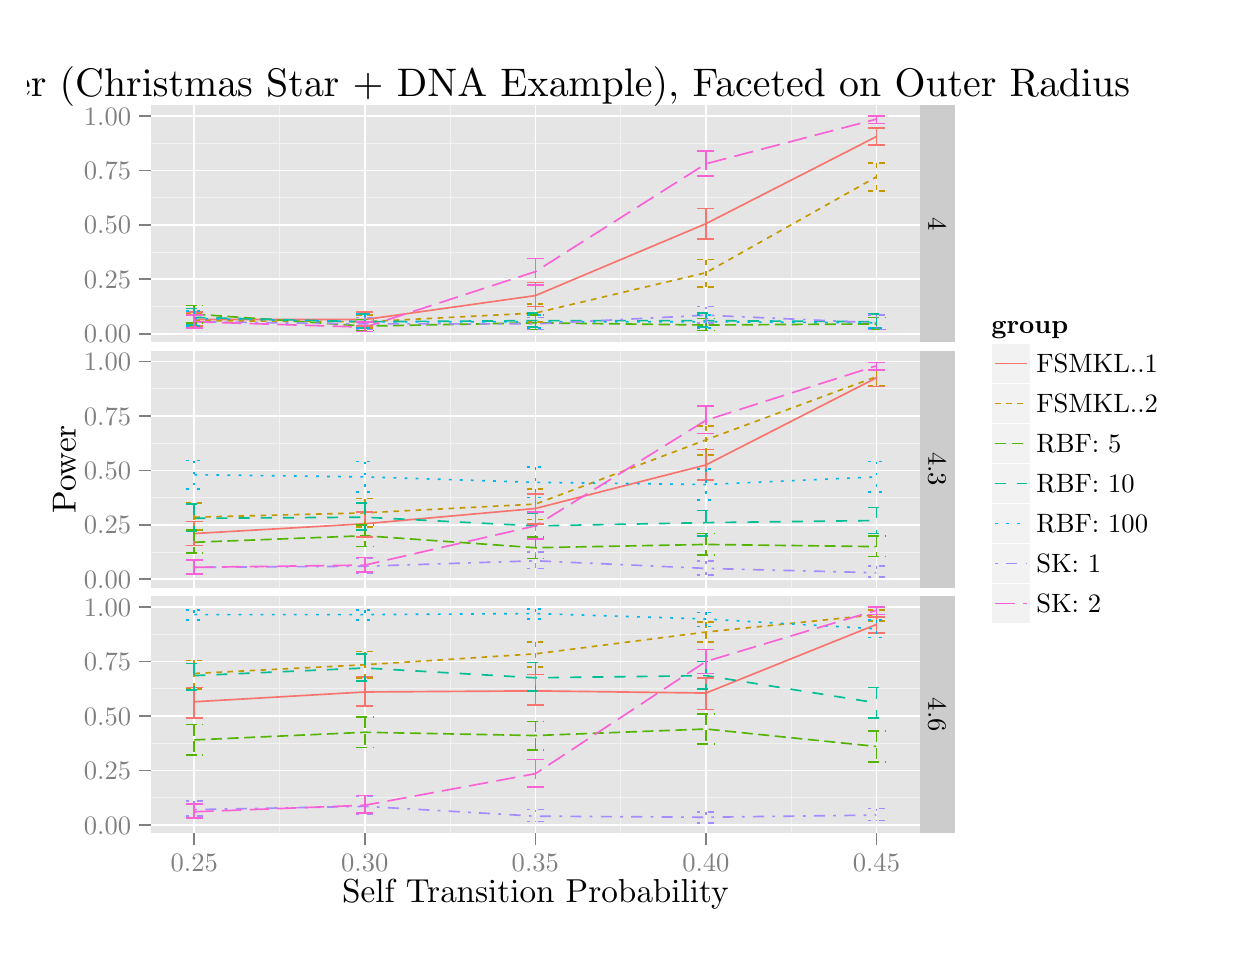
\begin{tikzpicture}[x=1pt,y=1pt]
\definecolor[named]{fillColor}{rgb}{1.00,1.00,1.00}
\path[use as bounding box,fill=fillColor,fill opacity=0.00] (0,0) rectangle (433.62,325.21);
\begin{scope}
\path[clip] (  0.00,  0.00) rectangle (433.62,325.21);
\definecolor[named]{drawColor}{rgb}{1.00,1.00,1.00}
\definecolor[named]{fillColor}{rgb}{1.00,1.00,1.00}

\path[draw=drawColor,line width= 0.6pt,line join=round,line cap=round,fill=fillColor] (  0.00,  0.00) rectangle (433.62,325.21);
\end{scope}
\begin{scope}
\path[clip] ( 44.49,211.51) rectangle (322.42,297.23);
\definecolor[named]{fillColor}{rgb}{0.90,0.90,0.90}

\path[fill=fillColor] ( 44.49,211.51) rectangle (322.42,297.23);
\definecolor[named]{drawColor}{rgb}{0.95,0.95,0.95}

\path[draw=drawColor,line width= 0.3pt,line join=round] ( 44.49,224.45) --
	(322.42,224.45);

\path[draw=drawColor,line width= 0.3pt,line join=round] ( 44.49,244.13) --
	(322.42,244.13);

\path[draw=drawColor,line width= 0.3pt,line join=round] ( 44.49,263.81) --
	(322.42,263.81);

\path[draw=drawColor,line width= 0.3pt,line join=round] ( 44.49,283.49) --
	(322.42,283.49);

\path[draw=drawColor,line width= 0.3pt,line join=round] ( 91.01,211.51) --
	( 91.01,297.23);

\path[draw=drawColor,line width= 0.3pt,line join=round] (152.64,211.51) --
	(152.64,297.23);

\path[draw=drawColor,line width= 0.3pt,line join=round] (214.27,211.51) --
	(214.27,297.23);

\path[draw=drawColor,line width= 0.3pt,line join=round] (275.89,211.51) --
	(275.89,297.23);
\definecolor[named]{drawColor}{rgb}{1.00,1.00,1.00}

\path[draw=drawColor,line width= 0.6pt,line join=round] ( 44.49,214.62) --
	(322.42,214.62);

\path[draw=drawColor,line width= 0.6pt,line join=round] ( 44.49,234.29) --
	(322.42,234.29);

\path[draw=drawColor,line width= 0.6pt,line join=round] ( 44.49,253.97) --
	(322.42,253.97);

\path[draw=drawColor,line width= 0.6pt,line join=round] ( 44.49,273.65) --
	(322.42,273.65);

\path[draw=drawColor,line width= 0.6pt,line join=round] ( 44.49,293.33) --
	(322.42,293.33);

\path[draw=drawColor,line width= 0.6pt,line join=round] ( 60.20,211.51) --
	( 60.20,297.23);

\path[draw=drawColor,line width= 0.6pt,line join=round] (121.83,211.51) --
	(121.83,297.23);

\path[draw=drawColor,line width= 0.6pt,line join=round] (183.45,211.51) --
	(183.45,297.23);

\path[draw=drawColor,line width= 0.6pt,line join=round] (245.08,211.51) --
	(245.08,297.23);

\path[draw=drawColor,line width= 0.6pt,line join=round] (306.70,211.51) --
	(306.70,297.23);
\definecolor[named]{drawColor}{rgb}{0.97,0.46,0.43}

\path[draw=drawColor,line width= 0.6pt,line join=round] ( 60.20,219.73) --
	(121.83,219.73) --
	(183.45,228.39) --
	(245.08,254.37) --
	(306.70,285.86);
\definecolor[named]{drawColor}{rgb}{0.77,0.60,0.00}

\path[draw=drawColor,line width= 0.6pt,dash pattern=on 2pt off 2pt ,line join=round] ( 60.20,219.34) --
	(121.83,218.94) --
	(183.45,222.09) --
	(245.08,236.66) --
	(306.70,271.29);
\definecolor[named]{drawColor}{rgb}{0.33,0.71,0.00}

\path[draw=drawColor,line width= 0.6pt,dash pattern=on 4pt off 2pt ,line join=round] ( 60.20,221.70) --
	(121.83,217.37) --
	(183.45,218.55) --
	(245.08,217.76) --
	(306.70,218.16);
\definecolor[named]{drawColor}{rgb}{0.00,0.75,0.58}

\path[draw=drawColor,line width= 0.6pt,dash pattern=on 4pt off 4pt ,line join=round] ( 60.20,220.52) --
	(121.83,218.94) --
	(183.45,219.34) --
	(245.08,219.34) --
	(306.70,218.94);
\definecolor[named]{drawColor}{rgb}{0.00,0.71,0.92}

\path[draw=drawColor,line width= 0.6pt,dash pattern=on 1pt off 3pt ,line join=round] ( 60.20,220.13) --
	(121.83,218.94) --
	(183.45,218.94) --
	(245.08,218.94) --
	(306.70,218.55);
\definecolor[named]{drawColor}{rgb}{0.65,0.54,1.00}

\path[draw=drawColor,line width= 0.6pt,dash pattern=on 1pt off 3pt on 4pt off 3pt ,line join=round] ( 60.20,218.94) --
	(121.83,218.16) --
	(183.45,218.16) --
	(245.08,221.31) --
	(306.70,218.55);
\definecolor[named]{drawColor}{rgb}{0.98,0.38,0.84}

\path[draw=drawColor,line width= 0.6pt,dash pattern=on 7pt off 3pt ,line join=round] ( 60.20,218.94) --
	(121.83,216.98) --
	(183.45,237.05) --
	(245.08,276.02) --
	(306.70,292.15);
\definecolor[named]{drawColor}{rgb}{0.97,0.46,0.43}

\path[draw=drawColor,line width= 0.6pt,line join=round] ( 57.12,222.49) --
	( 63.28,222.49);

\path[draw=drawColor,line width= 0.6pt,line join=round] ( 60.20,222.49) --
	( 60.20,217.36);

\path[draw=drawColor,line width= 0.6pt,line join=round] ( 57.12,217.36) --
	( 63.28,217.36);

\path[draw=drawColor,line width= 0.6pt,line join=round] (118.74,222.49) --
	(124.91,222.49);

\path[draw=drawColor,line width= 0.6pt,line join=round] (121.83,222.49) --
	(121.83,217.37);

\path[draw=drawColor,line width= 0.6pt,line join=round] (118.74,217.37) --
	(124.91,217.37);

\path[draw=drawColor,line width= 0.6pt,line join=round] (180.37,233.11) --
	(186.53,233.11);

\path[draw=drawColor,line width= 0.6pt,line join=round] (183.45,233.11) --
	(183.45,224.45);

\path[draw=drawColor,line width= 0.6pt,line join=round] (180.37,224.45) --
	(186.53,224.45);

\path[draw=drawColor,line width= 0.6pt,line join=round] (242.00,259.88) --
	(248.16,259.88);

\path[draw=drawColor,line width= 0.6pt,line join=round] (245.08,259.88) --
	(245.08,248.86);

\path[draw=drawColor,line width= 0.6pt,line join=round] (242.00,248.86) --
	(248.16,248.86);

\path[draw=drawColor,line width= 0.6pt,line join=round] (303.62,289.00) --
	(309.79,289.00);

\path[draw=drawColor,line width= 0.6pt,line join=round] (306.70,289.00) --
	(306.70,282.71);

\path[draw=drawColor,line width= 0.6pt,line join=round] (303.62,282.71) --
	(309.79,282.71);
\definecolor[named]{drawColor}{rgb}{0.77,0.60,0.00}

\path[draw=drawColor,line width= 0.6pt,dash pattern=on 2pt off 2pt ,line join=round] ( 57.12,221.70) --
	( 63.28,221.70);

\path[draw=drawColor,line width= 0.6pt,dash pattern=on 2pt off 2pt ,line join=round] ( 60.20,221.70) --
	( 60.20,216.98);

\path[draw=drawColor,line width= 0.6pt,dash pattern=on 2pt off 2pt ,line join=round] ( 57.12,216.98) --
	( 63.28,216.98);

\path[draw=drawColor,line width= 0.6pt,dash pattern=on 2pt off 2pt ,line join=round] (118.74,221.32) --
	(124.91,221.32);

\path[draw=drawColor,line width= 0.6pt,dash pattern=on 2pt off 2pt ,line join=round] (121.83,221.32) --
	(121.83,216.58);

\path[draw=drawColor,line width= 0.6pt,dash pattern=on 2pt off 2pt ,line join=round] (118.74,216.58) --
	(124.91,216.58);

\path[draw=drawColor,line width= 0.6pt,dash pattern=on 2pt off 2pt ,line join=round] (180.37,225.25) --
	(186.53,225.25);

\path[draw=drawColor,line width= 0.6pt,dash pattern=on 2pt off 2pt ,line join=round] (183.45,225.25) --
	(183.45,218.94);

\path[draw=drawColor,line width= 0.6pt,dash pattern=on 2pt off 2pt ,line join=round] (180.37,218.94) --
	(186.53,218.94);

\path[draw=drawColor,line width= 0.6pt,dash pattern=on 2pt off 2pt ,line join=round] (242.00,241.38) --
	(248.16,241.38);

\path[draw=drawColor,line width= 0.6pt,dash pattern=on 2pt off 2pt ,line join=round] (245.08,241.38) --
	(245.08,231.54);

\path[draw=drawColor,line width= 0.6pt,dash pattern=on 2pt off 2pt ,line join=round] (242.00,231.54) --
	(248.16,231.54);

\path[draw=drawColor,line width= 0.6pt,dash pattern=on 2pt off 2pt ,line join=round] (303.62,276.41) --
	(309.79,276.41);

\path[draw=drawColor,line width= 0.6pt,dash pattern=on 2pt off 2pt ,line join=round] (306.70,276.41) --
	(306.70,266.17);

\path[draw=drawColor,line width= 0.6pt,dash pattern=on 2pt off 2pt ,line join=round] (303.62,266.17) --
	(309.79,266.17);
\definecolor[named]{drawColor}{rgb}{0.33,0.71,0.00}

\path[draw=drawColor,line width= 0.6pt,dash pattern=on 4pt off 2pt ,line join=round] ( 57.12,224.85) --
	( 63.28,224.85);

\path[draw=drawColor,line width= 0.6pt,dash pattern=on 4pt off 2pt ,line join=round] ( 60.20,224.85) --
	( 60.20,218.55);

\path[draw=drawColor,line width= 0.6pt,dash pattern=on 4pt off 2pt ,line join=round] ( 57.12,218.55) --
	( 63.28,218.55);

\path[draw=drawColor,line width= 0.6pt,dash pattern=on 4pt off 2pt ,line join=round] (118.74,219.73) --
	(124.91,219.73);

\path[draw=drawColor,line width= 0.6pt,dash pattern=on 4pt off 2pt ,line join=round] (121.83,219.73) --
	(121.83,215.80);

\path[draw=drawColor,line width= 0.6pt,dash pattern=on 4pt off 2pt ,line join=round] (118.74,215.80) --
	(124.91,215.80);

\path[draw=drawColor,line width= 0.6pt,dash pattern=on 4pt off 2pt ,line join=round] (180.37,221.31) --
	(186.53,221.31);

\path[draw=drawColor,line width= 0.6pt,dash pattern=on 4pt off 2pt ,line join=round] (183.45,221.31) --
	(183.45,216.19);

\path[draw=drawColor,line width= 0.6pt,dash pattern=on 4pt off 2pt ,line join=round] (180.37,216.19) --
	(186.53,216.19);

\path[draw=drawColor,line width= 0.6pt,dash pattern=on 4pt off 2pt ,line join=round] (242.00,220.13) --
	(248.16,220.13);

\path[draw=drawColor,line width= 0.6pt,dash pattern=on 4pt off 2pt ,line join=round] (245.08,220.13) --
	(245.08,215.80);

\path[draw=drawColor,line width= 0.6pt,dash pattern=on 4pt off 2pt ,line join=round] (242.00,215.80) --
	(248.16,215.80);

\path[draw=drawColor,line width= 0.6pt,dash pattern=on 4pt off 2pt ,line join=round] (303.62,220.52) --
	(309.79,220.52);

\path[draw=drawColor,line width= 0.6pt,dash pattern=on 4pt off 2pt ,line join=round] (306.70,220.52) --
	(306.70,216.19);

\path[draw=drawColor,line width= 0.6pt,dash pattern=on 4pt off 2pt ,line join=round] (303.62,216.19) --
	(309.79,216.19);
\definecolor[named]{drawColor}{rgb}{0.00,0.75,0.58}

\path[draw=drawColor,line width= 0.6pt,dash pattern=on 4pt off 4pt ,line join=round] ( 57.12,223.67) --
	( 63.28,223.67);

\path[draw=drawColor,line width= 0.6pt,dash pattern=on 4pt off 4pt ,line join=round] ( 60.20,223.67) --
	( 60.20,217.76);

\path[draw=drawColor,line width= 0.6pt,dash pattern=on 4pt off 4pt ,line join=round] ( 57.12,217.76) --
	( 63.28,217.76);

\path[draw=drawColor,line width= 0.6pt,dash pattern=on 4pt off 4pt ,line join=round] (118.74,221.70) --
	(124.91,221.70);

\path[draw=drawColor,line width= 0.6pt,dash pattern=on 4pt off 4pt ,line join=round] (121.83,221.70) --
	(121.83,216.58);

\path[draw=drawColor,line width= 0.6pt,dash pattern=on 4pt off 4pt ,line join=round] (118.74,216.58) --
	(124.91,216.58);

\path[draw=drawColor,line width= 0.6pt,dash pattern=on 4pt off 4pt ,line join=round] (180.37,222.09) --
	(186.53,222.09);

\path[draw=drawColor,line width= 0.6pt,dash pattern=on 4pt off 4pt ,line join=round] (183.45,222.09) --
	(183.45,216.98);

\path[draw=drawColor,line width= 0.6pt,dash pattern=on 4pt off 4pt ,line join=round] (180.37,216.98) --
	(186.53,216.98);

\path[draw=drawColor,line width= 0.6pt,dash pattern=on 4pt off 4pt ,line join=round] (242.00,222.09) --
	(248.16,222.09);

\path[draw=drawColor,line width= 0.6pt,dash pattern=on 4pt off 4pt ,line join=round] (245.08,222.09) --
	(245.08,216.98);

\path[draw=drawColor,line width= 0.6pt,dash pattern=on 4pt off 4pt ,line join=round] (242.00,216.98) --
	(248.16,216.98);

\path[draw=drawColor,line width= 0.6pt,dash pattern=on 4pt off 4pt ,line join=round] (303.62,221.70) --
	(309.79,221.70);

\path[draw=drawColor,line width= 0.6pt,dash pattern=on 4pt off 4pt ,line join=round] (306.70,221.70) --
	(306.70,216.58);

\path[draw=drawColor,line width= 0.6pt,dash pattern=on 4pt off 4pt ,line join=round] (303.62,216.58) --
	(309.79,216.58);
\definecolor[named]{drawColor}{rgb}{0.00,0.71,0.92}

\path[draw=drawColor,line width= 0.6pt,dash pattern=on 1pt off 3pt ,line join=round] ( 57.12,222.88) --
	( 63.28,222.88);

\path[draw=drawColor,line width= 0.6pt,dash pattern=on 1pt off 3pt ,line join=round] ( 60.20,222.88) --
	( 60.20,217.37);

\path[draw=drawColor,line width= 0.6pt,dash pattern=on 1pt off 3pt ,line join=round] ( 57.12,217.37) --
	( 63.28,217.37);

\path[draw=drawColor,line width= 0.6pt,dash pattern=on 1pt off 3pt ,line join=round] (118.74,221.70) --
	(124.91,221.70);

\path[draw=drawColor,line width= 0.6pt,dash pattern=on 1pt off 3pt ,line join=round] (121.83,221.70) --
	(121.83,216.58);

\path[draw=drawColor,line width= 0.6pt,dash pattern=on 1pt off 3pt ,line join=round] (118.74,216.58) --
	(124.91,216.58);

\path[draw=drawColor,line width= 0.6pt,dash pattern=on 1pt off 3pt ,line join=round] (180.37,221.31) --
	(186.53,221.31);

\path[draw=drawColor,line width= 0.6pt,dash pattern=on 1pt off 3pt ,line join=round] (183.45,221.31) --
	(183.45,216.58);

\path[draw=drawColor,line width= 0.6pt,dash pattern=on 1pt off 3pt ,line join=round] (180.37,216.58) --
	(186.53,216.58);

\path[draw=drawColor,line width= 0.6pt,dash pattern=on 1pt off 3pt ,line join=round] (242.00,221.32) --
	(248.16,221.32);

\path[draw=drawColor,line width= 0.6pt,dash pattern=on 1pt off 3pt ,line join=round] (245.08,221.32) --
	(245.08,216.58);

\path[draw=drawColor,line width= 0.6pt,dash pattern=on 1pt off 3pt ,line join=round] (242.00,216.58) --
	(248.16,216.58);

\path[draw=drawColor,line width= 0.6pt,dash pattern=on 1pt off 3pt ,line join=round] (303.62,221.31) --
	(309.79,221.31);

\path[draw=drawColor,line width= 0.6pt,dash pattern=on 1pt off 3pt ,line join=round] (306.70,221.31) --
	(306.70,216.57);

\path[draw=drawColor,line width= 0.6pt,dash pattern=on 1pt off 3pt ,line join=round] (303.62,216.57) --
	(309.79,216.57);
\definecolor[named]{drawColor}{rgb}{0.65,0.54,1.00}

\path[draw=drawColor,line width= 0.6pt,dash pattern=on 1pt off 3pt on 4pt off 3pt ,line join=round] ( 57.12,221.32) --
	( 63.28,221.32);

\path[draw=drawColor,line width= 0.6pt,dash pattern=on 1pt off 3pt on 4pt off 3pt ,line join=round] ( 60.20,221.32) --
	( 60.20,216.58);

\path[draw=drawColor,line width= 0.6pt,dash pattern=on 1pt off 3pt on 4pt off 3pt ,line join=round] ( 57.12,216.58) --
	( 63.28,216.58);

\path[draw=drawColor,line width= 0.6pt,dash pattern=on 1pt off 3pt on 4pt off 3pt ,line join=round] (118.74,220.52) --
	(124.91,220.52);

\path[draw=drawColor,line width= 0.6pt,dash pattern=on 1pt off 3pt on 4pt off 3pt ,line join=round] (121.83,220.52) --
	(121.83,216.19);

\path[draw=drawColor,line width= 0.6pt,dash pattern=on 1pt off 3pt on 4pt off 3pt ,line join=round] (118.74,216.19) --
	(124.91,216.19);

\path[draw=drawColor,line width= 0.6pt,dash pattern=on 1pt off 3pt on 4pt off 3pt ,line join=round] (180.37,220.52) --
	(186.53,220.52);

\path[draw=drawColor,line width= 0.6pt,dash pattern=on 1pt off 3pt on 4pt off 3pt ,line join=round] (183.45,220.52) --
	(183.45,216.19);

\path[draw=drawColor,line width= 0.6pt,dash pattern=on 1pt off 3pt on 4pt off 3pt ,line join=round] (180.37,216.19) --
	(186.53,216.19);

\path[draw=drawColor,line width= 0.6pt,dash pattern=on 1pt off 3pt on 4pt off 3pt ,line join=round] (242.00,224.45) --
	(248.16,224.45);

\path[draw=drawColor,line width= 0.6pt,dash pattern=on 1pt off 3pt on 4pt off 3pt ,line join=round] (245.08,224.45) --
	(245.08,218.55);

\path[draw=drawColor,line width= 0.6pt,dash pattern=on 1pt off 3pt on 4pt off 3pt ,line join=round] (242.00,218.55) --
	(248.16,218.55);

\path[draw=drawColor,line width= 0.6pt,dash pattern=on 1pt off 3pt on 4pt off 3pt ,line join=round] (303.62,221.31) --
	(309.79,221.31);

\path[draw=drawColor,line width= 0.6pt,dash pattern=on 1pt off 3pt on 4pt off 3pt ,line join=round] (306.70,221.31) --
	(306.70,216.19);

\path[draw=drawColor,line width= 0.6pt,dash pattern=on 1pt off 3pt on 4pt off 3pt ,line join=round] (303.62,216.19) --
	(309.79,216.19);
\definecolor[named]{drawColor}{rgb}{0.98,0.38,0.84}

\path[draw=drawColor,line width= 0.6pt,dash pattern=on 7pt off 3pt ,line join=round] ( 57.12,221.31) --
	( 63.28,221.31);

\path[draw=drawColor,line width= 0.6pt,dash pattern=on 7pt off 3pt ,line join=round] ( 60.20,221.31) --
	( 60.20,216.58);

\path[draw=drawColor,line width= 0.6pt,dash pattern=on 7pt off 3pt ,line join=round] ( 57.12,216.58) --
	( 63.28,216.58);

\path[draw=drawColor,line width= 0.6pt,dash pattern=on 7pt off 3pt ,line join=round] (118.74,218.94) --
	(124.91,218.94);

\path[draw=drawColor,line width= 0.6pt,dash pattern=on 7pt off 3pt ,line join=round] (121.83,218.94) --
	(121.83,215.40);

\path[draw=drawColor,line width= 0.6pt,dash pattern=on 7pt off 3pt ,line join=round] (118.74,215.40) --
	(124.91,215.40);

\path[draw=drawColor,line width= 0.6pt,dash pattern=on 7pt off 3pt ,line join=round] (180.37,241.77) --
	(186.53,241.77);

\path[draw=drawColor,line width= 0.6pt,dash pattern=on 7pt off 3pt ,line join=round] (183.45,241.77) --
	(183.45,232.33);

\path[draw=drawColor,line width= 0.6pt,dash pattern=on 7pt off 3pt ,line join=round] (180.37,232.33) --
	(186.53,232.33);

\path[draw=drawColor,line width= 0.6pt,dash pattern=on 7pt off 3pt ,line join=round] (242.00,280.74) --
	(248.16,280.74);

\path[draw=drawColor,line width= 0.6pt,dash pattern=on 7pt off 3pt ,line join=round] (245.08,280.74) --
	(245.08,271.69);

\path[draw=drawColor,line width= 0.6pt,dash pattern=on 7pt off 3pt ,line join=round] (242.00,271.69) --
	(248.16,271.69);

\path[draw=drawColor,line width= 0.6pt,dash pattern=on 7pt off 3pt ,line join=round] (303.62,293.33) --
	(309.79,293.33);

\path[draw=drawColor,line width= 0.6pt,dash pattern=on 7pt off 3pt ,line join=round] (306.70,293.33) --
	(306.70,290.58);

\path[draw=drawColor,line width= 0.6pt,dash pattern=on 7pt off 3pt ,line join=round] (303.62,290.58) --
	(309.79,290.58);
\end{scope}
\begin{scope}
\path[clip] ( 44.49,122.77) rectangle (322.42,208.49);
\definecolor[named]{fillColor}{rgb}{0.90,0.90,0.90}

\path[fill=fillColor] ( 44.49,122.77) rectangle (322.42,208.49);
\definecolor[named]{drawColor}{rgb}{0.95,0.95,0.95}

\path[draw=drawColor,line width= 0.3pt,line join=round] ( 44.49,135.72) --
	(322.42,135.72);

\path[draw=drawColor,line width= 0.3pt,line join=round] ( 44.49,155.40) --
	(322.42,155.40);

\path[draw=drawColor,line width= 0.3pt,line join=round] ( 44.49,175.08) --
	(322.42,175.08);

\path[draw=drawColor,line width= 0.3pt,line join=round] ( 44.49,194.76) --
	(322.42,194.76);

\path[draw=drawColor,line width= 0.3pt,line join=round] ( 91.01,122.77) --
	( 91.01,208.49);

\path[draw=drawColor,line width= 0.3pt,line join=round] (152.64,122.77) --
	(152.64,208.49);

\path[draw=drawColor,line width= 0.3pt,line join=round] (214.27,122.77) --
	(214.27,208.49);

\path[draw=drawColor,line width= 0.3pt,line join=round] (275.89,122.77) --
	(275.89,208.49);
\definecolor[named]{drawColor}{rgb}{1.00,1.00,1.00}

\path[draw=drawColor,line width= 0.6pt,line join=round] ( 44.49,125.88) --
	(322.42,125.88);

\path[draw=drawColor,line width= 0.6pt,line join=round] ( 44.49,145.56) --
	(322.42,145.56);

\path[draw=drawColor,line width= 0.6pt,line join=round] ( 44.49,165.24) --
	(322.42,165.24);

\path[draw=drawColor,line width= 0.6pt,line join=round] ( 44.49,184.92) --
	(322.42,184.92);

\path[draw=drawColor,line width= 0.6pt,line join=round] ( 44.49,204.60) --
	(322.42,204.60);

\path[draw=drawColor,line width= 0.6pt,line join=round] ( 60.20,122.77) --
	( 60.20,208.49);

\path[draw=drawColor,line width= 0.6pt,line join=round] (121.83,122.77) --
	(121.83,208.49);

\path[draw=drawColor,line width= 0.6pt,line join=round] (183.45,122.77) --
	(183.45,208.49);

\path[draw=drawColor,line width= 0.6pt,line join=round] (245.08,122.77) --
	(245.08,208.49);

\path[draw=drawColor,line width= 0.6pt,line join=round] (306.70,122.77) --
	(306.70,208.49);
\definecolor[named]{drawColor}{rgb}{0.97,0.46,0.43}

\path[draw=drawColor,line width= 0.6pt,line join=round] ( 60.20,142.41) --
	(121.83,145.95) --
	(183.45,151.46) --
	(245.08,167.21) --
	(306.70,198.69);
\definecolor[named]{drawColor}{rgb}{0.77,0.60,0.00}

\path[draw=drawColor,line width= 0.6pt,dash pattern=on 2pt off 2pt ,line join=round] ( 60.20,148.31) --
	(121.83,149.89) --
	(183.45,153.04) --
	(245.08,176.26) --
	(306.70,199.09);
\definecolor[named]{drawColor}{rgb}{0.33,0.71,0.00}

\path[draw=drawColor,line width= 0.6pt,dash pattern=on 4pt off 2pt ,line join=round] ( 60.20,139.26) --
	(121.83,141.62) --
	(183.45,137.29) --
	(245.08,138.47) --
	(306.70,137.69);
\definecolor[named]{drawColor}{rgb}{0.00,0.75,0.58}

\path[draw=drawColor,line width= 0.6pt,dash pattern=on 4pt off 4pt ,line join=round] ( 60.20,147.92) --
	(121.83,148.31) --
	(183.45,145.17) --
	(245.08,146.35) --
	(306.70,147.13);
\definecolor[named]{drawColor}{rgb}{0.00,0.71,0.92}

\path[draw=drawColor,line width= 0.6pt,dash pattern=on 1pt off 3pt ,line join=round] ( 60.20,163.66) --
	(121.83,162.88) --
	(183.45,160.91) --
	(245.08,160.12) --
	(306.70,162.88);
\definecolor[named]{drawColor}{rgb}{0.65,0.54,1.00}

\path[draw=drawColor,line width= 0.6pt,dash pattern=on 1pt off 3pt on 4pt off 3pt ,line join=round] ( 60.20,130.21) --
	(121.83,130.60) --
	(183.45,132.57) --
	(245.08,129.82) --
	(306.70,128.24);
\definecolor[named]{drawColor}{rgb}{0.98,0.38,0.84}

\path[draw=drawColor,line width= 0.6pt,dash pattern=on 7pt off 3pt ,line join=round] ( 60.20,130.21) --
	(121.83,131.00) --
	(183.45,145.17) --
	(245.08,183.34) --
	(306.70,203.02);
\definecolor[named]{drawColor}{rgb}{0.97,0.46,0.43}

\path[draw=drawColor,line width= 0.6pt,line join=round] ( 57.12,146.74) --
	( 63.28,146.74);

\path[draw=drawColor,line width= 0.6pt,line join=round] ( 60.20,146.74) --
	( 60.20,138.08);

\path[draw=drawColor,line width= 0.6pt,line join=round] ( 57.12,138.08) --
	( 63.28,138.08);

\path[draw=drawColor,line width= 0.6pt,line join=round] (118.74,150.28) --
	(124.91,150.28);

\path[draw=drawColor,line width= 0.6pt,line join=round] (121.83,150.28) --
	(121.83,141.23);

\path[draw=drawColor,line width= 0.6pt,line join=round] (118.74,141.23) --
	(124.91,141.23);

\path[draw=drawColor,line width= 0.6pt,line join=round] (180.37,156.59) --
	(186.53,156.59);

\path[draw=drawColor,line width= 0.6pt,line join=round] (183.45,156.59) --
	(183.45,145.95);

\path[draw=drawColor,line width= 0.6pt,line join=round] (180.37,145.95) --
	(186.53,145.95);

\path[draw=drawColor,line width= 0.6pt,line join=round] (242.00,172.73) --
	(248.16,172.73);

\path[draw=drawColor,line width= 0.6pt,line join=round] (245.08,172.73) --
	(245.08,161.69);

\path[draw=drawColor,line width= 0.6pt,line join=round] (242.00,161.69) --
	(248.16,161.69);

\path[draw=drawColor,line width= 0.6pt,line join=round] (303.62,201.45) --
	(309.79,201.45);

\path[draw=drawColor,line width= 0.6pt,line join=round] (306.70,201.45) --
	(306.70,195.55);

\path[draw=drawColor,line width= 0.6pt,line join=round] (303.62,195.55) --
	(309.79,195.55);
\definecolor[named]{drawColor}{rgb}{0.77,0.60,0.00}

\path[draw=drawColor,line width= 0.6pt,dash pattern=on 2pt off 2pt ,line join=round] ( 57.12,153.43) --
	( 63.28,153.43);

\path[draw=drawColor,line width= 0.6pt,dash pattern=on 2pt off 2pt ,line join=round] ( 60.20,153.43) --
	( 60.20,143.59);

\path[draw=drawColor,line width= 0.6pt,dash pattern=on 2pt off 2pt ,line join=round] ( 57.12,143.59) --
	( 63.28,143.59);

\path[draw=drawColor,line width= 0.6pt,dash pattern=on 2pt off 2pt ,line join=round] (118.74,155.02) --
	(124.91,155.02);

\path[draw=drawColor,line width= 0.6pt,dash pattern=on 2pt off 2pt ,line join=round] (121.83,155.02) --
	(121.83,144.77);

\path[draw=drawColor,line width= 0.6pt,dash pattern=on 2pt off 2pt ,line join=round] (118.74,144.77) --
	(124.91,144.77);

\path[draw=drawColor,line width= 0.6pt,dash pattern=on 2pt off 2pt ,line join=round] (180.37,158.55) --
	(186.53,158.55);

\path[draw=drawColor,line width= 0.6pt,dash pattern=on 2pt off 2pt ,line join=round] (183.45,158.55) --
	(183.45,147.53);

\path[draw=drawColor,line width= 0.6pt,dash pattern=on 2pt off 2pt ,line join=round] (180.37,147.53) --
	(186.53,147.53);

\path[draw=drawColor,line width= 0.6pt,dash pattern=on 2pt off 2pt ,line join=round] (242.00,181.38) --
	(248.16,181.38);

\path[draw=drawColor,line width= 0.6pt,dash pattern=on 2pt off 2pt ,line join=round] (245.08,181.38) --
	(245.08,170.75);

\path[draw=drawColor,line width= 0.6pt,dash pattern=on 2pt off 2pt ,line join=round] (242.00,170.75) --
	(248.16,170.75);

\path[draw=drawColor,line width= 0.6pt,dash pattern=on 2pt off 2pt ,line join=round] (303.62,201.45) --
	(309.79,201.45);

\path[draw=drawColor,line width= 0.6pt,dash pattern=on 2pt off 2pt ,line join=round] (306.70,201.45) --
	(306.70,195.94);

\path[draw=drawColor,line width= 0.6pt,dash pattern=on 2pt off 2pt ,line join=round] (303.62,195.94) --
	(309.79,195.94);
\definecolor[named]{drawColor}{rgb}{0.33,0.71,0.00}

\path[draw=drawColor,line width= 0.6pt,dash pattern=on 4pt off 2pt ,line join=round] ( 57.12,143.59) --
	( 63.28,143.59);

\path[draw=drawColor,line width= 0.6pt,dash pattern=on 4pt off 2pt ,line join=round] ( 60.20,143.59) --
	( 60.20,135.33);

\path[draw=drawColor,line width= 0.6pt,dash pattern=on 4pt off 2pt ,line join=round] ( 57.12,135.33) --
	( 63.28,135.33);

\path[draw=drawColor,line width= 0.6pt,dash pattern=on 4pt off 2pt ,line join=round] (118.74,145.57) --
	(124.91,145.57);

\path[draw=drawColor,line width= 0.6pt,dash pattern=on 4pt off 2pt ,line join=round] (121.83,145.57) --
	(121.83,137.69);

\path[draw=drawColor,line width= 0.6pt,dash pattern=on 4pt off 2pt ,line join=round] (118.74,137.69) --
	(124.91,137.69);

\path[draw=drawColor,line width= 0.6pt,dash pattern=on 4pt off 2pt ,line join=round] (180.37,141.23) --
	(186.53,141.23);

\path[draw=drawColor,line width= 0.6pt,dash pattern=on 4pt off 2pt ,line join=round] (183.45,141.23) --
	(183.45,133.36);

\path[draw=drawColor,line width= 0.6pt,dash pattern=on 4pt off 2pt ,line join=round] (180.37,133.36) --
	(186.53,133.36);

\path[draw=drawColor,line width= 0.6pt,dash pattern=on 4pt off 2pt ,line join=round] (242.00,142.42) --
	(248.16,142.42);

\path[draw=drawColor,line width= 0.6pt,dash pattern=on 4pt off 2pt ,line join=round] (245.08,142.42) --
	(245.08,134.54);

\path[draw=drawColor,line width= 0.6pt,dash pattern=on 4pt off 2pt ,line join=round] (242.00,134.54) --
	(248.16,134.54);

\path[draw=drawColor,line width= 0.6pt,dash pattern=on 4pt off 2pt ,line join=round] (303.62,141.62) --
	(309.79,141.62);

\path[draw=drawColor,line width= 0.6pt,dash pattern=on 4pt off 2pt ,line join=round] (306.70,141.62) --
	(306.70,134.14);

\path[draw=drawColor,line width= 0.6pt,dash pattern=on 4pt off 2pt ,line join=round] (303.62,134.14) --
	(309.79,134.14);
\definecolor[named]{drawColor}{rgb}{0.00,0.75,0.58}

\path[draw=drawColor,line width= 0.6pt,dash pattern=on 4pt off 4pt ,line join=round] ( 57.12,153.04) --
	( 63.28,153.04);

\path[draw=drawColor,line width= 0.6pt,dash pattern=on 4pt off 4pt ,line join=round] ( 60.20,153.04) --
	( 60.20,143.20);

\path[draw=drawColor,line width= 0.6pt,dash pattern=on 4pt off 4pt ,line join=round] ( 57.12,143.20) --
	( 63.28,143.20);

\path[draw=drawColor,line width= 0.6pt,dash pattern=on 4pt off 4pt ,line join=round] (118.74,153.43) --
	(124.91,153.43);

\path[draw=drawColor,line width= 0.6pt,dash pattern=on 4pt off 4pt ,line join=round] (121.83,153.43) --
	(121.83,143.59);

\path[draw=drawColor,line width= 0.6pt,dash pattern=on 4pt off 4pt ,line join=round] (118.74,143.59) --
	(124.91,143.59);

\path[draw=drawColor,line width= 0.6pt,dash pattern=on 4pt off 4pt ,line join=round] (180.37,149.89) --
	(186.53,149.89);

\path[draw=drawColor,line width= 0.6pt,dash pattern=on 4pt off 4pt ,line join=round] (183.45,149.89) --
	(183.45,140.44);

\path[draw=drawColor,line width= 0.6pt,dash pattern=on 4pt off 4pt ,line join=round] (180.37,140.44) --
	(186.53,140.44);

\path[draw=drawColor,line width= 0.6pt,dash pattern=on 4pt off 4pt ,line join=round] (242.00,150.68) --
	(248.16,150.68);

\path[draw=drawColor,line width= 0.6pt,dash pattern=on 4pt off 4pt ,line join=round] (245.08,150.68) --
	(245.08,141.62);

\path[draw=drawColor,line width= 0.6pt,dash pattern=on 4pt off 4pt ,line join=round] (242.00,141.62) --
	(248.16,141.62);

\path[draw=drawColor,line width= 0.6pt,dash pattern=on 4pt off 4pt ,line join=round] (303.62,151.86) --
	(309.79,151.86);

\path[draw=drawColor,line width= 0.6pt,dash pattern=on 4pt off 4pt ,line join=round] (306.70,151.86) --
	(306.70,142.40);

\path[draw=drawColor,line width= 0.6pt,dash pattern=on 4pt off 4pt ,line join=round] (303.62,142.40) --
	(309.79,142.40);
\definecolor[named]{drawColor}{rgb}{0.00,0.71,0.92}

\path[draw=drawColor,line width= 0.6pt,dash pattern=on 1pt off 3pt ,line join=round] ( 57.12,168.78) --
	( 63.28,168.78);

\path[draw=drawColor,line width= 0.6pt,dash pattern=on 1pt off 3pt ,line join=round] ( 60.20,168.78) --
	( 60.20,158.54);

\path[draw=drawColor,line width= 0.6pt,dash pattern=on 1pt off 3pt ,line join=round] ( 57.12,158.54) --
	( 63.28,158.54);

\path[draw=drawColor,line width= 0.6pt,dash pattern=on 1pt off 3pt ,line join=round] (118.74,168.39) --
	(124.91,168.39);

\path[draw=drawColor,line width= 0.6pt,dash pattern=on 1pt off 3pt ,line join=round] (121.83,168.39) --
	(121.83,157.37);

\path[draw=drawColor,line width= 0.6pt,dash pattern=on 1pt off 3pt ,line join=round] (118.74,157.37) --
	(124.91,157.37);

\path[draw=drawColor,line width= 0.6pt,dash pattern=on 1pt off 3pt ,line join=round] (180.37,166.42) --
	(186.53,166.42);

\path[draw=drawColor,line width= 0.6pt,dash pattern=on 1pt off 3pt ,line join=round] (183.45,166.42) --
	(183.45,155.40);

\path[draw=drawColor,line width= 0.6pt,dash pattern=on 1pt off 3pt ,line join=round] (180.37,155.40) --
	(186.53,155.40);

\path[draw=drawColor,line width= 0.6pt,dash pattern=on 1pt off 3pt ,line join=round] (242.00,165.63) --
	(248.16,165.63);

\path[draw=drawColor,line width= 0.6pt,dash pattern=on 1pt off 3pt ,line join=round] (245.08,165.63) --
	(245.08,154.61);

\path[draw=drawColor,line width= 0.6pt,dash pattern=on 1pt off 3pt ,line join=round] (242.00,154.61) --
	(248.16,154.61);

\path[draw=drawColor,line width= 0.6pt,dash pattern=on 1pt off 3pt ,line join=round] (303.62,168.39) --
	(309.79,168.39);

\path[draw=drawColor,line width= 0.6pt,dash pattern=on 1pt off 3pt ,line join=round] (306.70,168.39) --
	(306.70,157.37);

\path[draw=drawColor,line width= 0.6pt,dash pattern=on 1pt off 3pt ,line join=round] (303.62,157.37) --
	(309.79,157.37);
\definecolor[named]{drawColor}{rgb}{0.65,0.54,1.00}

\path[draw=drawColor,line width= 0.6pt,dash pattern=on 1pt off 3pt on 4pt off 3pt ,line join=round] ( 57.12,132.96) --
	( 63.28,132.96);

\path[draw=drawColor,line width= 0.6pt,dash pattern=on 1pt off 3pt on 4pt off 3pt ,line join=round] ( 60.20,132.96) --
	( 60.20,127.85);

\path[draw=drawColor,line width= 0.6pt,dash pattern=on 1pt off 3pt on 4pt off 3pt ,line join=round] ( 57.12,127.85) --
	( 63.28,127.85);

\path[draw=drawColor,line width= 0.6pt,dash pattern=on 1pt off 3pt on 4pt off 3pt ,line join=round] (118.74,133.36) --
	(124.91,133.36);

\path[draw=drawColor,line width= 0.6pt,dash pattern=on 1pt off 3pt on 4pt off 3pt ,line join=round] (121.83,133.36) --
	(121.83,128.24);

\path[draw=drawColor,line width= 0.6pt,dash pattern=on 1pt off 3pt on 4pt off 3pt ,line join=round] (118.74,128.24) --
	(124.91,128.24);

\path[draw=drawColor,line width= 0.6pt,dash pattern=on 1pt off 3pt on 4pt off 3pt ,line join=round] (180.37,135.72) --
	(186.53,135.72);

\path[draw=drawColor,line width= 0.6pt,dash pattern=on 1pt off 3pt on 4pt off 3pt ,line join=round] (183.45,135.72) --
	(183.45,129.82);

\path[draw=drawColor,line width= 0.6pt,dash pattern=on 1pt off 3pt on 4pt off 3pt ,line join=round] (180.37,129.82) --
	(186.53,129.82);

\path[draw=drawColor,line width= 0.6pt,dash pattern=on 1pt off 3pt on 4pt off 3pt ,line join=round] (242.00,132.57) --
	(248.16,132.57);

\path[draw=drawColor,line width= 0.6pt,dash pattern=on 1pt off 3pt on 4pt off 3pt ,line join=round] (245.08,132.57) --
	(245.08,127.45);

\path[draw=drawColor,line width= 0.6pt,dash pattern=on 1pt off 3pt on 4pt off 3pt ,line join=round] (242.00,127.45) --
	(248.16,127.45);

\path[draw=drawColor,line width= 0.6pt,dash pattern=on 1pt off 3pt on 4pt off 3pt ,line join=round] (303.62,130.60) --
	(309.79,130.60);

\path[draw=drawColor,line width= 0.6pt,dash pattern=on 1pt off 3pt on 4pt off 3pt ,line join=round] (306.70,130.60) --
	(306.70,126.67);

\path[draw=drawColor,line width= 0.6pt,dash pattern=on 1pt off 3pt on 4pt off 3pt ,line join=round] (303.62,126.67) --
	(309.79,126.67);
\definecolor[named]{drawColor}{rgb}{0.98,0.38,0.84}

\path[draw=drawColor,line width= 0.6pt,dash pattern=on 7pt off 3pt ,line join=round] ( 57.12,132.96) --
	( 63.28,132.96);

\path[draw=drawColor,line width= 0.6pt,dash pattern=on 7pt off 3pt ,line join=round] ( 60.20,132.96) --
	( 60.20,127.85);

\path[draw=drawColor,line width= 0.6pt,dash pattern=on 7pt off 3pt ,line join=round] ( 57.12,127.85) --
	( 63.28,127.85);

\path[draw=drawColor,line width= 0.6pt,dash pattern=on 7pt off 3pt ,line join=round] (118.74,133.75) --
	(124.91,133.75);

\path[draw=drawColor,line width= 0.6pt,dash pattern=on 7pt off 3pt ,line join=round] (121.83,133.75) --
	(121.83,128.62);

\path[draw=drawColor,line width= 0.6pt,dash pattern=on 7pt off 3pt ,line join=round] (118.74,128.62) --
	(124.91,128.62);

\path[draw=drawColor,line width= 0.6pt,dash pattern=on 7pt off 3pt ,line join=round] (180.37,150.28) --
	(186.53,150.28);

\path[draw=drawColor,line width= 0.6pt,dash pattern=on 7pt off 3pt ,line join=round] (183.45,150.28) --
	(183.45,140.44);

\path[draw=drawColor,line width= 0.6pt,dash pattern=on 7pt off 3pt ,line join=round] (180.37,140.44) --
	(186.53,140.44);

\path[draw=drawColor,line width= 0.6pt,dash pattern=on 7pt off 3pt ,line join=round] (242.00,188.46) --
	(248.16,188.46);

\path[draw=drawColor,line width= 0.6pt,dash pattern=on 7pt off 3pt ,line join=round] (245.08,188.46) --
	(245.08,178.62);

\path[draw=drawColor,line width= 0.6pt,dash pattern=on 7pt off 3pt ,line join=round] (242.00,178.62) --
	(248.16,178.62);

\path[draw=drawColor,line width= 0.6pt,dash pattern=on 7pt off 3pt ,line join=round] (303.62,204.20) --
	(309.79,204.20);

\path[draw=drawColor,line width= 0.6pt,dash pattern=on 7pt off 3pt ,line join=round] (306.70,204.20) --
	(306.70,201.45);

\path[draw=drawColor,line width= 0.6pt,dash pattern=on 7pt off 3pt ,line join=round] (303.62,201.45) --
	(309.79,201.45);
\end{scope}
\begin{scope}
\path[clip] ( 44.49, 34.03) rectangle (322.42,119.76);
\definecolor[named]{fillColor}{rgb}{0.90,0.90,0.90}

\path[fill=fillColor] ( 44.49, 34.03) rectangle (322.42,119.76);
\definecolor[named]{drawColor}{rgb}{0.95,0.95,0.95}

\path[draw=drawColor,line width= 0.3pt,line join=round] ( 44.49, 46.98) --
	(322.42, 46.98);

\path[draw=drawColor,line width= 0.3pt,line join=round] ( 44.49, 66.66) --
	(322.42, 66.66);

\path[draw=drawColor,line width= 0.3pt,line join=round] ( 44.49, 86.34) --
	(322.42, 86.34);

\path[draw=drawColor,line width= 0.3pt,line join=round] ( 44.49,106.02) --
	(322.42,106.02);

\path[draw=drawColor,line width= 0.3pt,line join=round] ( 91.01, 34.03) --
	( 91.01,119.76);

\path[draw=drawColor,line width= 0.3pt,line join=round] (152.64, 34.03) --
	(152.64,119.76);

\path[draw=drawColor,line width= 0.3pt,line join=round] (214.27, 34.03) --
	(214.27,119.76);

\path[draw=drawColor,line width= 0.3pt,line join=round] (275.89, 34.03) --
	(275.89,119.76);
\definecolor[named]{drawColor}{rgb}{1.00,1.00,1.00}

\path[draw=drawColor,line width= 0.6pt,line join=round] ( 44.49, 37.14) --
	(322.42, 37.14);

\path[draw=drawColor,line width= 0.6pt,line join=round] ( 44.49, 56.82) --
	(322.42, 56.82);

\path[draw=drawColor,line width= 0.6pt,line join=round] ( 44.49, 76.50) --
	(322.42, 76.50);

\path[draw=drawColor,line width= 0.6pt,line join=round] ( 44.49, 96.18) --
	(322.42, 96.18);

\path[draw=drawColor,line width= 0.6pt,line join=round] ( 44.49,115.86) --
	(322.42,115.86);

\path[draw=drawColor,line width= 0.6pt,line join=round] ( 60.20, 34.03) --
	( 60.20,119.76);

\path[draw=drawColor,line width= 0.6pt,line join=round] (121.83, 34.03) --
	(121.83,119.76);

\path[draw=drawColor,line width= 0.6pt,line join=round] (183.45, 34.03) --
	(183.45,119.76);

\path[draw=drawColor,line width= 0.6pt,line join=round] (245.08, 34.03) --
	(245.08,119.76);

\path[draw=drawColor,line width= 0.6pt,line join=round] (306.70, 34.03) --
	(306.70,119.76);
\definecolor[named]{drawColor}{rgb}{0.97,0.46,0.43}

\path[draw=drawColor,line width= 0.6pt,line join=round] ( 60.20, 81.62) --
	(121.83, 85.16) --
	(183.45, 85.56) --
	(245.08, 84.77) --
	(306.70,109.56);
\definecolor[named]{drawColor}{rgb}{0.77,0.60,0.00}

\path[draw=drawColor,line width= 0.6pt,dash pattern=on 2pt off 2pt ,line join=round] ( 60.20, 91.85) --
	(121.83, 95.00) --
	(183.45, 98.94) --
	(245.08,106.81) --
	(306.70,113.11);
\definecolor[named]{drawColor}{rgb}{0.33,0.71,0.00}

\path[draw=drawColor,line width= 0.6pt,dash pattern=on 4pt off 2pt ,line join=round] ( 60.20, 67.84) --
	(121.83, 70.60) --
	(183.45, 69.42) --
	(245.08, 71.78) --
	(306.70, 65.48);
\definecolor[named]{drawColor}{rgb}{0.00,0.75,0.58}

\path[draw=drawColor,line width= 0.6pt,dash pattern=on 4pt off 4pt ,line join=round] ( 60.20, 91.07) --
	(121.83, 93.82) --
	(183.45, 90.28) --
	(245.08, 91.07) --
	(306.70, 81.23);
\definecolor[named]{drawColor}{rgb}{0.00,0.71,0.92}

\path[draw=drawColor,line width= 0.6pt,dash pattern=on 1pt off 3pt ,line join=round] ( 60.20,113.11) --
	(121.83,113.11) --
	(183.45,113.50) --
	(245.08,111.53) --
	(306.70,107.99);
\definecolor[named]{drawColor}{rgb}{0.65,0.54,1.00}

\path[draw=drawColor,line width= 0.6pt,dash pattern=on 1pt off 3pt on 4pt off 3pt ,line join=round] ( 60.20, 42.65) --
	(121.83, 43.84) --
	(183.45, 40.29) --
	(245.08, 39.90) --
	(306.70, 40.69);
\definecolor[named]{drawColor}{rgb}{0.98,0.38,0.84}

\path[draw=drawColor,line width= 0.6pt,dash pattern=on 7pt off 3pt ,line join=round] ( 60.20, 41.87) --
	(121.83, 44.23) --
	(183.45, 55.64) --
	(245.08, 96.18) --
	(306.70,114.68);
\definecolor[named]{drawColor}{rgb}{0.97,0.46,0.43}

\path[draw=drawColor,line width= 0.6pt,line join=round] ( 57.12, 86.74) --
	( 63.28, 86.74);

\path[draw=drawColor,line width= 0.6pt,line join=round] ( 60.20, 86.74) --
	( 60.20, 75.72);

\path[draw=drawColor,line width= 0.6pt,line join=round] ( 57.12, 75.72) --
	( 63.28, 75.72);

\path[draw=drawColor,line width= 0.6pt,line join=round] (118.74, 90.67) --
	(124.91, 90.67);

\path[draw=drawColor,line width= 0.6pt,line join=round] (121.83, 90.67) --
	(121.83, 80.05);

\path[draw=drawColor,line width= 0.6pt,line join=round] (118.74, 80.05) --
	(124.91, 80.05);

\path[draw=drawColor,line width= 0.6pt,line join=round] (180.37, 91.46) --
	(186.53, 91.46);

\path[draw=drawColor,line width= 0.6pt,line join=round] (183.45, 91.46) --
	(183.45, 80.44);

\path[draw=drawColor,line width= 0.6pt,line join=round] (180.37, 80.44) --
	(186.53, 80.44);

\path[draw=drawColor,line width= 0.6pt,line join=round] (242.00, 90.28) --
	(248.16, 90.28);

\path[draw=drawColor,line width= 0.6pt,line join=round] (245.08, 90.28) --
	(245.08, 78.86);

\path[draw=drawColor,line width= 0.6pt,line join=round] (242.00, 78.86) --
	(248.16, 78.86);

\path[draw=drawColor,line width= 0.6pt,line join=round] (303.62,112.32) --
	(309.79,112.32);

\path[draw=drawColor,line width= 0.6pt,line join=round] (306.70,112.32) --
	(306.70,106.42);

\path[draw=drawColor,line width= 0.6pt,line join=round] (303.62,106.42) --
	(309.79,106.42);
\definecolor[named]{drawColor}{rgb}{0.77,0.60,0.00}

\path[draw=drawColor,line width= 0.6pt,dash pattern=on 2pt off 2pt ,line join=round] ( 57.12, 96.58) --
	( 63.28, 96.58);

\path[draw=drawColor,line width= 0.6pt,dash pattern=on 2pt off 2pt ,line join=round] ( 60.20, 96.58) --
	( 60.20, 86.34);

\path[draw=drawColor,line width= 0.6pt,dash pattern=on 2pt off 2pt ,line join=round] ( 57.12, 86.34) --
	( 63.28, 86.34);

\path[draw=drawColor,line width= 0.6pt,dash pattern=on 2pt off 2pt ,line join=round] (118.74, 99.73) --
	(124.91, 99.73);

\path[draw=drawColor,line width= 0.6pt,dash pattern=on 2pt off 2pt ,line join=round] (121.83, 99.73) --
	(121.83, 90.28);

\path[draw=drawColor,line width= 0.6pt,dash pattern=on 2pt off 2pt ,line join=round] (118.74, 90.28) --
	(124.91, 90.28);

\path[draw=drawColor,line width= 0.6pt,dash pattern=on 2pt off 2pt ,line join=round] (180.37,103.27) --
	(186.53,103.27);

\path[draw=drawColor,line width= 0.6pt,dash pattern=on 2pt off 2pt ,line join=round] (183.45,103.27) --
	(183.45, 94.21);

\path[draw=drawColor,line width= 0.6pt,dash pattern=on 2pt off 2pt ,line join=round] (180.37, 94.21) --
	(186.53, 94.21);

\path[draw=drawColor,line width= 0.6pt,dash pattern=on 2pt off 2pt ,line join=round] (242.00,110.35) --
	(248.16,110.35);

\path[draw=drawColor,line width= 0.6pt,dash pattern=on 2pt off 2pt ,line join=round] (245.08,110.35) --
	(245.08,103.27);

\path[draw=drawColor,line width= 0.6pt,dash pattern=on 2pt off 2pt ,line join=round] (242.00,103.27) --
	(248.16,103.27);

\path[draw=drawColor,line width= 0.6pt,dash pattern=on 2pt off 2pt ,line join=round] (303.62,114.68) --
	(309.79,114.68);

\path[draw=drawColor,line width= 0.6pt,dash pattern=on 2pt off 2pt ,line join=round] (306.70,114.68) --
	(306.70,110.75);

\path[draw=drawColor,line width= 0.6pt,dash pattern=on 2pt off 2pt ,line join=round] (303.62,110.75) --
	(309.79,110.75);
\definecolor[named]{drawColor}{rgb}{0.33,0.71,0.00}

\path[draw=drawColor,line width= 0.6pt,dash pattern=on 4pt off 2pt ,line join=round] ( 57.12, 73.35) --
	( 63.28, 73.35);

\path[draw=drawColor,line width= 0.6pt,dash pattern=on 4pt off 2pt ,line join=round] ( 60.20, 73.35) --
	( 60.20, 62.33);

\path[draw=drawColor,line width= 0.6pt,dash pattern=on 4pt off 2pt ,line join=round] ( 57.12, 62.33) --
	( 63.28, 62.33);

\path[draw=drawColor,line width= 0.6pt,dash pattern=on 4pt off 2pt ,line join=round] (118.74, 76.11) --
	(124.91, 76.11);

\path[draw=drawColor,line width= 0.6pt,dash pattern=on 4pt off 2pt ,line join=round] (121.83, 76.11) --
	(121.83, 65.09);

\path[draw=drawColor,line width= 0.6pt,dash pattern=on 4pt off 2pt ,line join=round] (118.74, 65.09) --
	(124.91, 65.09);

\path[draw=drawColor,line width= 0.6pt,dash pattern=on 4pt off 2pt ,line join=round] (180.37, 74.54) --
	(186.53, 74.54);

\path[draw=drawColor,line width= 0.6pt,dash pattern=on 4pt off 2pt ,line join=round] (183.45, 74.54) --
	(183.45, 64.30);

\path[draw=drawColor,line width= 0.6pt,dash pattern=on 4pt off 2pt ,line join=round] (180.37, 64.30) --
	(186.53, 64.30);

\path[draw=drawColor,line width= 0.6pt,dash pattern=on 4pt off 2pt ,line join=round] (242.00, 77.29) --
	(248.16, 77.29);

\path[draw=drawColor,line width= 0.6pt,dash pattern=on 4pt off 2pt ,line join=round] (245.08, 77.29) --
	(245.08, 66.27);

\path[draw=drawColor,line width= 0.6pt,dash pattern=on 4pt off 2pt ,line join=round] (242.00, 66.27) --
	(248.16, 66.27);

\path[draw=drawColor,line width= 0.6pt,dash pattern=on 4pt off 2pt ,line join=round] (303.62, 70.99) --
	(309.79, 70.99);

\path[draw=drawColor,line width= 0.6pt,dash pattern=on 4pt off 2pt ,line join=round] (306.70, 70.99) --
	(306.70, 59.97);

\path[draw=drawColor,line width= 0.6pt,dash pattern=on 4pt off 2pt ,line join=round] (303.62, 59.97) --
	(309.79, 59.97);
\definecolor[named]{drawColor}{rgb}{0.00,0.75,0.58}

\path[draw=drawColor,line width= 0.6pt,dash pattern=on 4pt off 4pt ,line join=round] ( 57.12, 95.41) --
	( 63.28, 95.41);

\path[draw=drawColor,line width= 0.6pt,dash pattern=on 4pt off 4pt ,line join=round] ( 60.20, 95.41) --
	( 60.20, 85.95);

\path[draw=drawColor,line width= 0.6pt,dash pattern=on 4pt off 4pt ,line join=round] ( 57.12, 85.95) --
	( 63.28, 85.95);

\path[draw=drawColor,line width= 0.6pt,dash pattern=on 4pt off 4pt ,line join=round] (118.74, 98.94) --
	(124.91, 98.94);

\path[draw=drawColor,line width= 0.6pt,dash pattern=on 4pt off 4pt ,line join=round] (121.83, 98.94) --
	(121.83, 89.10);

\path[draw=drawColor,line width= 0.6pt,dash pattern=on 4pt off 4pt ,line join=round] (118.74, 89.10) --
	(124.91, 89.10);

\path[draw=drawColor,line width= 0.6pt,dash pattern=on 4pt off 4pt ,line join=round] (180.37, 95.79) --
	(186.53, 95.79);

\path[draw=drawColor,line width= 0.6pt,dash pattern=on 4pt off 4pt ,line join=round] (183.45, 95.79) --
	(183.45, 85.56);

\path[draw=drawColor,line width= 0.6pt,dash pattern=on 4pt off 4pt ,line join=round] (180.37, 85.56) --
	(186.53, 85.56);

\path[draw=drawColor,line width= 0.6pt,dash pattern=on 4pt off 4pt ,line join=round] (242.00, 96.18) --
	(248.16, 96.18);

\path[draw=drawColor,line width= 0.6pt,dash pattern=on 4pt off 4pt ,line join=round] (245.08, 96.18) --
	(245.08, 86.34);

\path[draw=drawColor,line width= 0.6pt,dash pattern=on 4pt off 4pt ,line join=round] (242.00, 86.34) --
	(248.16, 86.34);

\path[draw=drawColor,line width= 0.6pt,dash pattern=on 4pt off 4pt ,line join=round] (303.62, 86.74) --
	(309.79, 86.74);

\path[draw=drawColor,line width= 0.6pt,dash pattern=on 4pt off 4pt ,line join=round] (306.70, 86.74) --
	(306.70, 75.72);

\path[draw=drawColor,line width= 0.6pt,dash pattern=on 4pt off 4pt ,line join=round] (303.62, 75.72) --
	(309.79, 75.72);
\definecolor[named]{drawColor}{rgb}{0.00,0.71,0.92}

\path[draw=drawColor,line width= 0.6pt,dash pattern=on 1pt off 3pt ,line join=round] ( 57.12,114.68) --
	( 63.28,114.68);

\path[draw=drawColor,line width= 0.6pt,dash pattern=on 1pt off 3pt ,line join=round] ( 60.20,114.68) --
	( 60.20,111.14);

\path[draw=drawColor,line width= 0.6pt,dash pattern=on 1pt off 3pt ,line join=round] ( 57.12,111.14) --
	( 63.28,111.14);

\path[draw=drawColor,line width= 0.6pt,dash pattern=on 1pt off 3pt ,line join=round] (118.74,114.69) --
	(124.91,114.69);

\path[draw=drawColor,line width= 0.6pt,dash pattern=on 1pt off 3pt ,line join=round] (121.83,114.69) --
	(121.83,111.14);

\path[draw=drawColor,line width= 0.6pt,dash pattern=on 1pt off 3pt ,line join=round] (118.74,111.14) --
	(124.91,111.14);

\path[draw=drawColor,line width= 0.6pt,dash pattern=on 1pt off 3pt ,line join=round] (180.37,115.08) --
	(186.53,115.08);

\path[draw=drawColor,line width= 0.6pt,dash pattern=on 1pt off 3pt ,line join=round] (183.45,115.08) --
	(183.45,111.53);

\path[draw=drawColor,line width= 0.6pt,dash pattern=on 1pt off 3pt ,line join=round] (180.37,111.53) --
	(186.53,111.53);

\path[draw=drawColor,line width= 0.6pt,dash pattern=on 1pt off 3pt ,line join=round] (242.00,113.89) --
	(248.16,113.89);

\path[draw=drawColor,line width= 0.6pt,dash pattern=on 1pt off 3pt ,line join=round] (245.08,113.89) --
	(245.08,108.78);

\path[draw=drawColor,line width= 0.6pt,dash pattern=on 1pt off 3pt ,line join=round] (242.00,108.78) --
	(248.16,108.78);

\path[draw=drawColor,line width= 0.6pt,dash pattern=on 1pt off 3pt ,line join=round] (303.62,111.14) --
	(309.79,111.14);

\path[draw=drawColor,line width= 0.6pt,dash pattern=on 1pt off 3pt ,line join=round] (306.70,111.14) --
	(306.70,104.84);

\path[draw=drawColor,line width= 0.6pt,dash pattern=on 1pt off 3pt ,line join=round] (303.62,104.84) --
	(309.79,104.84);
\definecolor[named]{drawColor}{rgb}{0.65,0.54,1.00}

\path[draw=drawColor,line width= 0.6pt,dash pattern=on 1pt off 3pt on 4pt off 3pt ,line join=round] ( 57.12, 45.80) --
	( 63.28, 45.80);

\path[draw=drawColor,line width= 0.6pt,dash pattern=on 1pt off 3pt on 4pt off 3pt ,line join=round] ( 60.20, 45.80) --
	( 60.20, 40.29);

\path[draw=drawColor,line width= 0.6pt,dash pattern=on 1pt off 3pt on 4pt off 3pt ,line join=round] ( 57.12, 40.29) --
	( 63.28, 40.29);

\path[draw=drawColor,line width= 0.6pt,dash pattern=on 1pt off 3pt on 4pt off 3pt ,line join=round] (118.74, 47.38) --
	(124.91, 47.38);

\path[draw=drawColor,line width= 0.6pt,dash pattern=on 1pt off 3pt on 4pt off 3pt ,line join=round] (121.83, 47.38) --
	(121.83, 41.08);

\path[draw=drawColor,line width= 0.6pt,dash pattern=on 1pt off 3pt on 4pt off 3pt ,line join=round] (118.74, 41.08) --
	(124.91, 41.08);

\path[draw=drawColor,line width= 0.6pt,dash pattern=on 1pt off 3pt on 4pt off 3pt ,line join=round] (180.37, 42.65) --
	(186.53, 42.65);

\path[draw=drawColor,line width= 0.6pt,dash pattern=on 1pt off 3pt on 4pt off 3pt ,line join=round] (183.45, 42.65) --
	(183.45, 38.32);

\path[draw=drawColor,line width= 0.6pt,dash pattern=on 1pt off 3pt on 4pt off 3pt ,line join=round] (180.37, 38.32) --
	(186.53, 38.32);

\path[draw=drawColor,line width= 0.6pt,dash pattern=on 1pt off 3pt on 4pt off 3pt ,line join=round] (242.00, 41.87) --
	(248.16, 41.87);

\path[draw=drawColor,line width= 0.6pt,dash pattern=on 1pt off 3pt on 4pt off 3pt ,line join=round] (245.08, 41.87) --
	(245.08, 37.93);

\path[draw=drawColor,line width= 0.6pt,dash pattern=on 1pt off 3pt on 4pt off 3pt ,line join=round] (242.00, 37.93) --
	(248.16, 37.93);

\path[draw=drawColor,line width= 0.6pt,dash pattern=on 1pt off 3pt on 4pt off 3pt ,line join=round] (303.62, 43.05) --
	(309.79, 43.05);

\path[draw=drawColor,line width= 0.6pt,dash pattern=on 1pt off 3pt on 4pt off 3pt ,line join=round] (306.70, 43.05) --
	(306.70, 38.72);

\path[draw=drawColor,line width= 0.6pt,dash pattern=on 1pt off 3pt on 4pt off 3pt ,line join=round] (303.62, 38.72) --
	(309.79, 38.72);
\definecolor[named]{drawColor}{rgb}{0.98,0.38,0.84}

\path[draw=drawColor,line width= 0.6pt,dash pattern=on 7pt off 3pt ,line join=round] ( 57.12, 44.62) --
	( 63.28, 44.62);

\path[draw=drawColor,line width= 0.6pt,dash pattern=on 7pt off 3pt ,line join=round] ( 60.20, 44.62) --
	( 60.20, 39.51);

\path[draw=drawColor,line width= 0.6pt,dash pattern=on 7pt off 3pt ,line join=round] ( 57.12, 39.51) --
	( 63.28, 39.51);

\path[draw=drawColor,line width= 0.6pt,dash pattern=on 7pt off 3pt ,line join=round] (118.74, 47.77) --
	(124.91, 47.77);

\path[draw=drawColor,line width= 0.6pt,dash pattern=on 7pt off 3pt ,line join=round] (121.83, 47.77) --
	(121.83, 41.47);

\path[draw=drawColor,line width= 0.6pt,dash pattern=on 7pt off 3pt ,line join=round] (118.74, 41.47) --
	(124.91, 41.47);

\path[draw=drawColor,line width= 0.6pt,dash pattern=on 7pt off 3pt ,line join=round] (180.37, 60.76) --
	(186.53, 60.76);

\path[draw=drawColor,line width= 0.6pt,dash pattern=on 7pt off 3pt ,line join=round] (183.45, 60.76) --
	(183.45, 50.92);

\path[draw=drawColor,line width= 0.6pt,dash pattern=on 7pt off 3pt ,line join=round] (180.37, 50.92) --
	(186.53, 50.92);

\path[draw=drawColor,line width= 0.6pt,dash pattern=on 7pt off 3pt ,line join=round] (242.00,100.51) --
	(248.16,100.51);

\path[draw=drawColor,line width= 0.6pt,dash pattern=on 7pt off 3pt ,line join=round] (245.08,100.51) --
	(245.08, 91.85);

\path[draw=drawColor,line width= 0.6pt,dash pattern=on 7pt off 3pt ,line join=round] (242.00, 91.85) --
	(248.16, 91.85);

\path[draw=drawColor,line width= 0.6pt,dash pattern=on 7pt off 3pt ,line join=round] (303.62,115.86) --
	(309.79,115.86);

\path[draw=drawColor,line width= 0.6pt,dash pattern=on 7pt off 3pt ,line join=round] (306.70,115.86) --
	(306.70,113.11);

\path[draw=drawColor,line width= 0.6pt,dash pattern=on 7pt off 3pt ,line join=round] (303.62,113.11) --
	(309.79,113.11);
\end{scope}
\begin{scope}
\path[clip] (  0.00,  0.00) rectangle (433.62,325.21);
\definecolor[named]{drawColor}{rgb}{0.50,0.50,0.50}

\node[text=drawColor,anchor=base east,inner sep=0pt, outer sep=0pt, scale=  0.96] at ( 37.37,211.31) {0.00};

\node[text=drawColor,anchor=base east,inner sep=0pt, outer sep=0pt, scale=  0.96] at ( 37.37,230.99) {0.25};

\node[text=drawColor,anchor=base east,inner sep=0pt, outer sep=0pt, scale=  0.96] at ( 37.37,250.67) {0.50};

\node[text=drawColor,anchor=base east,inner sep=0pt, outer sep=0pt, scale=  0.96] at ( 37.37,270.35) {0.75};

\node[text=drawColor,anchor=base east,inner sep=0pt, outer sep=0pt, scale=  0.96] at ( 37.37,290.03) {1.00};
\end{scope}
\begin{scope}
\path[clip] (  0.00,  0.00) rectangle (433.62,325.21);
\definecolor[named]{drawColor}{rgb}{0.50,0.50,0.50}

\path[draw=drawColor,line width= 0.6pt,line join=round] ( 40.22,214.62) --
	( 44.49,214.62);

\path[draw=drawColor,line width= 0.6pt,line join=round] ( 40.22,234.29) --
	( 44.49,234.29);

\path[draw=drawColor,line width= 0.6pt,line join=round] ( 40.22,253.97) --
	( 44.49,253.97);

\path[draw=drawColor,line width= 0.6pt,line join=round] ( 40.22,273.65) --
	( 44.49,273.65);

\path[draw=drawColor,line width= 0.6pt,line join=round] ( 40.22,293.33) --
	( 44.49,293.33);
\end{scope}
\begin{scope}
\path[clip] (  0.00,  0.00) rectangle (433.62,325.21);
\definecolor[named]{drawColor}{rgb}{0.50,0.50,0.50}

\node[text=drawColor,anchor=base east,inner sep=0pt, outer sep=0pt, scale=  0.96] at ( 37.37,122.57) {0.00};

\node[text=drawColor,anchor=base east,inner sep=0pt, outer sep=0pt, scale=  0.96] at ( 37.37,142.25) {0.25};

\node[text=drawColor,anchor=base east,inner sep=0pt, outer sep=0pt, scale=  0.96] at ( 37.37,161.93) {0.50};

\node[text=drawColor,anchor=base east,inner sep=0pt, outer sep=0pt, scale=  0.96] at ( 37.37,181.61) {0.75};

\node[text=drawColor,anchor=base east,inner sep=0pt, outer sep=0pt, scale=  0.96] at ( 37.37,201.29) {1.00};
\end{scope}
\begin{scope}
\path[clip] (  0.00,  0.00) rectangle (433.62,325.21);
\definecolor[named]{drawColor}{rgb}{0.50,0.50,0.50}

\path[draw=drawColor,line width= 0.6pt,line join=round] ( 40.22,125.88) --
	( 44.49,125.88);

\path[draw=drawColor,line width= 0.6pt,line join=round] ( 40.22,145.56) --
	( 44.49,145.56);

\path[draw=drawColor,line width= 0.6pt,line join=round] ( 40.22,165.24) --
	( 44.49,165.24);

\path[draw=drawColor,line width= 0.6pt,line join=round] ( 40.22,184.92) --
	( 44.49,184.92);

\path[draw=drawColor,line width= 0.6pt,line join=round] ( 40.22,204.60) --
	( 44.49,204.60);
\end{scope}
\begin{scope}
\path[clip] (  0.00,  0.00) rectangle (433.62,325.21);
\definecolor[named]{drawColor}{rgb}{0.50,0.50,0.50}

\node[text=drawColor,anchor=base east,inner sep=0pt, outer sep=0pt, scale=  0.96] at ( 37.37, 33.84) {0.00};

\node[text=drawColor,anchor=base east,inner sep=0pt, outer sep=0pt, scale=  0.96] at ( 37.37, 53.52) {0.25};

\node[text=drawColor,anchor=base east,inner sep=0pt, outer sep=0pt, scale=  0.96] at ( 37.37, 73.20) {0.50};

\node[text=drawColor,anchor=base east,inner sep=0pt, outer sep=0pt, scale=  0.96] at ( 37.37, 92.88) {0.75};

\node[text=drawColor,anchor=base east,inner sep=0pt, outer sep=0pt, scale=  0.96] at ( 37.37,112.56) {1.00};
\end{scope}
\begin{scope}
\path[clip] (  0.00,  0.00) rectangle (433.62,325.21);
\definecolor[named]{drawColor}{rgb}{0.50,0.50,0.50}

\path[draw=drawColor,line width= 0.6pt,line join=round] ( 40.22, 37.14) --
	( 44.49, 37.14);

\path[draw=drawColor,line width= 0.6pt,line join=round] ( 40.22, 56.82) --
	( 44.49, 56.82);

\path[draw=drawColor,line width= 0.6pt,line join=round] ( 40.22, 76.50) --
	( 44.49, 76.50);

\path[draw=drawColor,line width= 0.6pt,line join=round] ( 40.22, 96.18) --
	( 44.49, 96.18);

\path[draw=drawColor,line width= 0.6pt,line join=round] ( 40.22,115.86) --
	( 44.49,115.86);
\end{scope}
\begin{scope}
\path[clip] (322.42,211.51) rectangle (335.05,297.23);
\definecolor[named]{fillColor}{rgb}{0.80,0.80,0.80}

\path[fill=fillColor] (322.42,211.51) rectangle (335.05,297.23);
\definecolor[named]{drawColor}{rgb}{0.00,0.00,0.00}

\node[text=drawColor,rotate=270.00,anchor=base,inner sep=0pt, outer sep=0pt, scale=  0.96] at (325.43,254.37) {4};
\end{scope}
\begin{scope}
\path[clip] (322.42,122.77) rectangle (335.05,208.49);
\definecolor[named]{fillColor}{rgb}{0.80,0.80,0.80}

\path[fill=fillColor] (322.42,122.77) rectangle (335.05,208.49);
\definecolor[named]{drawColor}{rgb}{0.00,0.00,0.00}

\node[text=drawColor,rotate=270.00,anchor=base,inner sep=0pt, outer sep=0pt, scale=  0.96] at (325.43,165.63) {4.3};
\end{scope}
\begin{scope}
\path[clip] (322.42, 34.03) rectangle (335.05,119.76);
\definecolor[named]{fillColor}{rgb}{0.80,0.80,0.80}

\path[fill=fillColor] (322.42, 34.03) rectangle (335.05,119.76);
\definecolor[named]{drawColor}{rgb}{0.00,0.00,0.00}

\node[text=drawColor,rotate=270.00,anchor=base,inner sep=0pt, outer sep=0pt, scale=  0.96] at (325.43, 76.90) {4.6};
\end{scope}
\begin{scope}
\path[clip] (  0.00,  0.00) rectangle (433.62,325.21);
\definecolor[named]{drawColor}{rgb}{0.50,0.50,0.50}

\path[draw=drawColor,line width= 0.6pt,line join=round] ( 60.20, 29.77) --
	( 60.20, 34.03);

\path[draw=drawColor,line width= 0.6pt,line join=round] (121.83, 29.77) --
	(121.83, 34.03);

\path[draw=drawColor,line width= 0.6pt,line join=round] (183.45, 29.77) --
	(183.45, 34.03);

\path[draw=drawColor,line width= 0.6pt,line join=round] (245.08, 29.77) --
	(245.08, 34.03);

\path[draw=drawColor,line width= 0.6pt,line join=round] (306.70, 29.77) --
	(306.70, 34.03);
\end{scope}
\begin{scope}
\path[clip] (  0.00,  0.00) rectangle (433.62,325.21);
\definecolor[named]{drawColor}{rgb}{0.50,0.50,0.50}

\node[text=drawColor,anchor=base,inner sep=0pt, outer sep=0pt, scale=  0.96] at ( 60.20, 20.31) {0.25};

\node[text=drawColor,anchor=base,inner sep=0pt, outer sep=0pt, scale=  0.96] at (121.83, 20.31) {0.30};

\node[text=drawColor,anchor=base,inner sep=0pt, outer sep=0pt, scale=  0.96] at (183.45, 20.31) {0.35};

\node[text=drawColor,anchor=base,inner sep=0pt, outer sep=0pt, scale=  0.96] at (245.08, 20.31) {0.40};

\node[text=drawColor,anchor=base,inner sep=0pt, outer sep=0pt, scale=  0.96] at (306.70, 20.31) {0.45};
\end{scope}
\begin{scope}
\path[clip] (  0.00,  0.00) rectangle (433.62,325.21);
\definecolor[named]{drawColor}{rgb}{0.00,0.00,0.00}

\node[text=drawColor,anchor=base,inner sep=0pt, outer sep=0pt, scale=  1.20] at (183.45,  9.03) {Self Transition Probability};
\end{scope}
\begin{scope}
\path[clip] (  0.00,  0.00) rectangle (433.62,325.21);
\definecolor[named]{drawColor}{rgb}{0.00,0.00,0.00}

\node[text=drawColor,rotate= 90.00,anchor=base,inner sep=0pt, outer sep=0pt, scale=  1.20] at ( 17.30,165.63) {Power};
\end{scope}
\begin{scope}
\path[clip] (  0.00,  0.00) rectangle (433.62,325.21);
\definecolor[named]{fillColor}{rgb}{1.00,1.00,1.00}

\path[fill=fillColor] (343.92,105.66) rectangle (412.71,225.61);
\end{scope}
\begin{scope}
\path[clip] (  0.00,  0.00) rectangle (433.62,325.21);
\definecolor[named]{drawColor}{rgb}{0.00,0.00,0.00}

\node[text=drawColor,anchor=base west,inner sep=0pt, outer sep=0pt, scale=  0.96] at (348.19,214.72) {\bfseries group};
\end{scope}
\begin{scope}
\path[clip] (  0.00,  0.00) rectangle (433.62,325.21);
\definecolor[named]{drawColor}{rgb}{1.00,1.00,1.00}
\definecolor[named]{fillColor}{rgb}{0.95,0.95,0.95}

\path[draw=drawColor,line width= 0.6pt,line join=round,line cap=round,fill=fillColor] (348.19,196.65) rectangle (362.64,211.10);
\end{scope}
\begin{scope}
\path[clip] (  0.00,  0.00) rectangle (433.62,325.21);
\definecolor[named]{drawColor}{rgb}{0.97,0.46,0.43}

\path[draw=drawColor,line width= 0.6pt,line join=round] (349.63,203.87) -- (361.20,203.87);
\end{scope}
\begin{scope}
\path[clip] (  0.00,  0.00) rectangle (433.62,325.21);
\definecolor[named]{drawColor}{rgb}{0.97,0.46,0.43}

\path[draw=drawColor,line width= 0.6pt,line join=round] (349.63,203.87) -- (361.20,203.87);
\end{scope}
\begin{scope}
\path[clip] (  0.00,  0.00) rectangle (433.62,325.21);
\definecolor[named]{drawColor}{rgb}{1.00,1.00,1.00}
\definecolor[named]{fillColor}{rgb}{0.95,0.95,0.95}

\path[draw=drawColor,line width= 0.6pt,line join=round,line cap=round,fill=fillColor] (348.19,182.19) rectangle (362.64,196.65);
\end{scope}
\begin{scope}
\path[clip] (  0.00,  0.00) rectangle (433.62,325.21);
\definecolor[named]{drawColor}{rgb}{0.77,0.60,0.00}

\path[draw=drawColor,line width= 0.6pt,dash pattern=on 2pt off 2pt ,line join=round] (349.63,189.42) -- (361.20,189.42);
\end{scope}
\begin{scope}
\path[clip] (  0.00,  0.00) rectangle (433.62,325.21);
\definecolor[named]{drawColor}{rgb}{0.77,0.60,0.00}

\path[draw=drawColor,line width= 0.6pt,dash pattern=on 2pt off 2pt ,line join=round] (349.63,189.42) -- (361.20,189.42);
\end{scope}
\begin{scope}
\path[clip] (  0.00,  0.00) rectangle (433.62,325.21);
\definecolor[named]{drawColor}{rgb}{1.00,1.00,1.00}
\definecolor[named]{fillColor}{rgb}{0.95,0.95,0.95}

\path[draw=drawColor,line width= 0.6pt,line join=round,line cap=round,fill=fillColor] (348.19,167.74) rectangle (362.64,182.19);
\end{scope}
\begin{scope}
\path[clip] (  0.00,  0.00) rectangle (433.62,325.21);
\definecolor[named]{drawColor}{rgb}{0.33,0.71,0.00}

\path[draw=drawColor,line width= 0.6pt,dash pattern=on 4pt off 2pt ,line join=round] (349.63,174.97) -- (361.20,174.97);
\end{scope}
\begin{scope}
\path[clip] (  0.00,  0.00) rectangle (433.62,325.21);
\definecolor[named]{drawColor}{rgb}{0.33,0.71,0.00}

\path[draw=drawColor,line width= 0.6pt,dash pattern=on 4pt off 2pt ,line join=round] (349.63,174.97) -- (361.20,174.97);
\end{scope}
\begin{scope}
\path[clip] (  0.00,  0.00) rectangle (433.62,325.21);
\definecolor[named]{drawColor}{rgb}{1.00,1.00,1.00}
\definecolor[named]{fillColor}{rgb}{0.95,0.95,0.95}

\path[draw=drawColor,line width= 0.6pt,line join=round,line cap=round,fill=fillColor] (348.19,153.29) rectangle (362.64,167.74);
\end{scope}
\begin{scope}
\path[clip] (  0.00,  0.00) rectangle (433.62,325.21);
\definecolor[named]{drawColor}{rgb}{0.00,0.75,0.58}

\path[draw=drawColor,line width= 0.6pt,dash pattern=on 4pt off 4pt ,line join=round] (349.63,160.51) -- (361.20,160.51);
\end{scope}
\begin{scope}
\path[clip] (  0.00,  0.00) rectangle (433.62,325.21);
\definecolor[named]{drawColor}{rgb}{0.00,0.75,0.58}

\path[draw=drawColor,line width= 0.6pt,dash pattern=on 4pt off 4pt ,line join=round] (349.63,160.51) -- (361.20,160.51);
\end{scope}
\begin{scope}
\path[clip] (  0.00,  0.00) rectangle (433.62,325.21);
\definecolor[named]{drawColor}{rgb}{1.00,1.00,1.00}
\definecolor[named]{fillColor}{rgb}{0.95,0.95,0.95}

\path[draw=drawColor,line width= 0.6pt,line join=round,line cap=round,fill=fillColor] (348.19,138.83) rectangle (362.64,153.29);
\end{scope}
\begin{scope}
\path[clip] (  0.00,  0.00) rectangle (433.62,325.21);
\definecolor[named]{drawColor}{rgb}{0.00,0.71,0.92}

\path[draw=drawColor,line width= 0.6pt,dash pattern=on 1pt off 3pt ,line join=round] (349.63,146.06) -- (361.20,146.06);
\end{scope}
\begin{scope}
\path[clip] (  0.00,  0.00) rectangle (433.62,325.21);
\definecolor[named]{drawColor}{rgb}{0.00,0.71,0.92}

\path[draw=drawColor,line width= 0.6pt,dash pattern=on 1pt off 3pt ,line join=round] (349.63,146.06) -- (361.20,146.06);
\end{scope}
\begin{scope}
\path[clip] (  0.00,  0.00) rectangle (433.62,325.21);
\definecolor[named]{drawColor}{rgb}{1.00,1.00,1.00}
\definecolor[named]{fillColor}{rgb}{0.95,0.95,0.95}

\path[draw=drawColor,line width= 0.6pt,line join=round,line cap=round,fill=fillColor] (348.19,124.38) rectangle (362.64,138.83);
\end{scope}
\begin{scope}
\path[clip] (  0.00,  0.00) rectangle (433.62,325.21);
\definecolor[named]{drawColor}{rgb}{0.65,0.54,1.00}

\path[draw=drawColor,line width= 0.6pt,dash pattern=on 1pt off 3pt on 4pt off 3pt ,line join=round] (349.63,131.60) -- (361.20,131.60);
\end{scope}
\begin{scope}
\path[clip] (  0.00,  0.00) rectangle (433.62,325.21);
\definecolor[named]{drawColor}{rgb}{0.65,0.54,1.00}

\path[draw=drawColor,line width= 0.6pt,dash pattern=on 1pt off 3pt on 4pt off 3pt ,line join=round] (349.63,131.60) -- (361.20,131.60);
\end{scope}
\begin{scope}
\path[clip] (  0.00,  0.00) rectangle (433.62,325.21);
\definecolor[named]{drawColor}{rgb}{1.00,1.00,1.00}
\definecolor[named]{fillColor}{rgb}{0.95,0.95,0.95}

\path[draw=drawColor,line width= 0.6pt,line join=round,line cap=round,fill=fillColor] (348.19,109.92) rectangle (362.64,124.38);
\end{scope}
\begin{scope}
\path[clip] (  0.00,  0.00) rectangle (433.62,325.21);
\definecolor[named]{drawColor}{rgb}{0.98,0.38,0.84}

\path[draw=drawColor,line width= 0.6pt,dash pattern=on 7pt off 3pt ,line join=round] (349.63,117.15) -- (361.20,117.15);
\end{scope}
\begin{scope}
\path[clip] (  0.00,  0.00) rectangle (433.62,325.21);
\definecolor[named]{drawColor}{rgb}{0.98,0.38,0.84}

\path[draw=drawColor,line width= 0.6pt,dash pattern=on 7pt off 3pt ,line join=round] (349.63,117.15) -- (361.20,117.15);
\end{scope}
\begin{scope}
\path[clip] (  0.00,  0.00) rectangle (433.62,325.21);
\definecolor[named]{drawColor}{rgb}{0.00,0.00,0.00}

\node[text=drawColor,anchor=base west,inner sep=0pt, outer sep=0pt, scale=  0.96] at (364.45,200.57) {FSMKL..1};
\end{scope}
\begin{scope}
\path[clip] (  0.00,  0.00) rectangle (433.62,325.21);
\definecolor[named]{drawColor}{rgb}{0.00,0.00,0.00}

\node[text=drawColor,anchor=base west,inner sep=0pt, outer sep=0pt, scale=  0.96] at (364.45,186.12) {FSMKL..2};
\end{scope}
\begin{scope}
\path[clip] (  0.00,  0.00) rectangle (433.62,325.21);
\definecolor[named]{drawColor}{rgb}{0.00,0.00,0.00}

\node[text=drawColor,anchor=base west,inner sep=0pt, outer sep=0pt, scale=  0.96] at (364.45,171.66) {RBF: 5};
\end{scope}
\begin{scope}
\path[clip] (  0.00,  0.00) rectangle (433.62,325.21);
\definecolor[named]{drawColor}{rgb}{0.00,0.00,0.00}

\node[text=drawColor,anchor=base west,inner sep=0pt, outer sep=0pt, scale=  0.96] at (364.45,157.21) {RBF: 10};
\end{scope}
\begin{scope}
\path[clip] (  0.00,  0.00) rectangle (433.62,325.21);
\definecolor[named]{drawColor}{rgb}{0.00,0.00,0.00}

\node[text=drawColor,anchor=base west,inner sep=0pt, outer sep=0pt, scale=  0.96] at (364.45,142.75) {RBF: 100};
\end{scope}
\begin{scope}
\path[clip] (  0.00,  0.00) rectangle (433.62,325.21);
\definecolor[named]{drawColor}{rgb}{0.00,0.00,0.00}

\node[text=drawColor,anchor=base west,inner sep=0pt, outer sep=0pt, scale=  0.96] at (364.45,128.30) {SK: 1};
\end{scope}
\begin{scope}
\path[clip] (  0.00,  0.00) rectangle (433.62,325.21);
\definecolor[named]{drawColor}{rgb}{0.00,0.00,0.00}

\node[text=drawColor,anchor=base west,inner sep=0pt, outer sep=0pt, scale=  0.96] at (364.45,113.85) {SK: 2};
\end{scope}
\begin{scope}
\path[clip] (  0.00,  0.00) rectangle (433.62,325.21);
\definecolor[named]{drawColor}{rgb}{0.00,0.00,0.00}

\node[text=drawColor,anchor=base,inner sep=0pt, outer sep=0pt, scale=  1.44] at (183.45,300.24) {Power (Christmas Star + DNA Example), Faceted on Outer Radius};
\end{scope}
\end{tikzpicture}

    }
  \end{center}
\end{frame}

\begin{frame}{Future Work}
  \begin{itemize}
  \item Generalize theory for higher dimensional settings and/or
    non-linear scoring functions \pause
  \item Develop similarities with Hotelling's $T^2$-test \pause
  \item Explore performance on different types of data, in particular,
    unstructured data such as images \pause
  \item Heterogeneous data: optimal combinations of kernels
    via SDPs, KL divergence \pause
  \end{itemize}
\end{frame}

\begin{frame}[allowframebreaks]{References}
  \bibliographystyle{ieeetr}
  \bibliography{ncray}
\end{frame}

\end{document}
